\documentclass[11pt]{book}
\oddsidemargin 0in
\evensidemargin 0in
\marginparwidth 0in
\textheight 8in
\textwidth 6.5in
\topmargin 0in
\headheight 14pt
\usepackage{amssymb,amsmath,amsthm,fancyhdr,supertabular,longtable,hhline,mathtools}
\usepackage{colortbl}
\usepackage{import, multicol,boxedminipage}
\usepackage{chapterfolder}
\usepackage[metapost,truebbox]{mfpic}
\usepackage[pdflatex]{graphicx}
\usepackage{makeidx}
\usepackage[colorlinks, hyperindex, plainpages=false, linkcolor=blue, urlcolor=blue, pdfpagelabels]{hyperref}
\usepackage[all]{hypcap}
\usepackage{cancel}
\usepackage{sectsty}
\usepackage{textcomp}
\allsectionsfont{\mdseries \scshape}
\definecolor{ResultColor}{gray}{0.9}
\theoremstyle{definition}  % this prevents the text in definitions, theorems, and corollaries from being italicized
\newtheorem{defn}{\sc Definition}[chapter]
\newtheorem{thm}{\sc Theorem}[chapter]
\newtheorem{cor}[thm]{\sc Corollary}
\newtheorem{eqn}{\sc Equation}[chapter]
\newtheorem{ex}{\sc Example}[section]
\newtheorem{fig}{\sc Figure}[chapter]
\setlength{\parindent}{0in}
\newcommand{\bbm}{\begin{boxedminipage}{6.41in}}
\newcommand{\ebm}{\end{boxedminipage}}
\newcommand{\ds}{\displaystyle}
\usepackage{array}
\setlength{\extrarowheight}{2pt}
\allowdisplaybreaks[2]
\allsectionsfont{\mdseries \scshape}
%Below is for Helvetica (scaled): 
\usepackage[scaled=.92]{helvet}   
\renewcommand{\familydefault}{\sfdefault}  %makes the text of the book sans serif
\usepackage[helvet]{sfmath}  %makes the math in the book sans serif
\allsectionsfont{\sffamily}  %makes the chapter and section titles sans serif

\makeatletter
\newcases{mycases}{\quad}{%
  \hfil$\m@th\displaystyle{##}$}{$\m@th\displaystyle{##}$\hfil}{\lbrace}{.}
\makeatother

\begin{document}
\newcounter{HW}
\newcounter{HWindent}
\renewcommand{\textinterrobang}{$! \! \! ?$}


\chapter{\sc  Root, Radical and Power Functions}

\section{Root and Radical Functions}

\mfpicnumber{1}

\opengraphsfile{RootRadicalFunctions}

\setcounter{footnote}{0}

\label{RootRadicalFunctions}

In Sections \ref{ConstantandLinearFunctions}, \ref{AbsoluteValueFunctions} and \ref{QuadraticFunctions}, we studied constant, linear,  absolute value,\footnote{These were introduced, as you may recall, as piecewise-defined linear functions.} and quadratic functions.  Constant, linear and quadratic functions were specific examples of polynomial functions, which we studied in generality in Chapter \ref{PolynomialFunctions}. Chapter \ref{PolynomialFunctions} culminated with the Real Factorization Theorem, Theorem \ref{realfactorization}, which says that all polynomial functions with real coefficients can be thought of as products of linear and quadratic functions.  Our next step was to enlarge our field\footnote{This is a really bad math pun.} of study to rational functions in Chapter \ref{RationalFunctions}.  Being quotients of polynomials, we can ultimately view this family of functions as being built up of linear and quadratic functions as well.  So in some sense, Sections   \ref{ConstantandLinearFunctions}, \ref{AbsoluteValueFunctions} and \ref{QuadraticFunctions} along with Chapters \ref{PolynomialFunctions} and \ref{RationalFunctions} can be thought of as an exhaustive study of linear and quadratic\footnote{If we broaden our concept of functions to allow for complex valued coefficients, the Complex Factorization Theorem, Theorem \ref{complexfactorization}, tells us every function we have studied thus far is a combination of linear functions.} functions.  We now turn our attention to functions involving radicals which cannot be written in terms of linear functions.  For a more detailed review of the basics of roots and radicals, we refer the reader to Sections \ref{AppRealNumberArithmetic} and  \ref{AppRadEqus}.  




\subsection{Root Functions}
\label{RootFunctions}

As with polynomial functions and rational functions, we begin our study of functions involving radical with a special family of functions: the (principal) root functions.

\smallskip

\colorbox{ResultColor}{\bbm

\begin{defn} \label{principalrootfunction}  Let $n \in \mathbb{N}$ with $n \geq 2$.  The \index{$n$th root function}\index{function, $n$th root} \textbf{$n$ th (principal) root function} is the function $f(x) = \sqrt[n]{x}$.  

\textbf{NOTE:}  If $n$ is even, the domain of $f$ is $[0, \infty)$;  if $n$ is odd, the domain of $f$ is $(-\infty, \infty)$.

\end{defn}

\ebm}

\smallskip

The domain restriction for even indexed roots means that, once again, we are restricting our attention to \textit{real} numbers.\footnote{Although we discussed imaginary numbers in Section \ref{ComplexZeros}, we restrict our attention to real numbers in this section.  See the epilogue on page \pageref{complexepilogue} for more details.}  We graph a few members of the root function family below, and quickly notice that, as with the monomial, and, more generally, the Laurent monomial functions, the behavior of the root functions depends primarily on whether the root is even or odd.  

In addition to having the common domain of $[0, \infty)$, the graphs of $f(x) = \sqrt[n]{x}$ for even indices $n$ all share the points $(0,0)$ and $(1,1)$. As $n$ increases, the functions become `steeper' near the $y$-axis and `flatter' as $x \rightarrow \infty$.  To show $f(x) \rightarrow \infty$ as $x \rightarrow \infty$, we show, more generally, the range of $f$ is $[0, \infty)$.  Indeed, if $c \geq 0$ is a real number, then $f(c^n) = \sqrt[n]{c^n} = c$ so $c$ is in the range of $f$.  Note that $f$ is increasing:  that is, if $a<b$, then $f(a) = \sqrt[n]{a} < \sqrt[n]{b} = f(b)$. This property is useful in solving certain types of polynomial inequalities.\footnote{See Exercise \ref{rootstosolvepolyineq}.}

\begin{tabular}{ccc}

\begin{mfpic}[15]{0}{9}{0}{3}
\axes
\tlabel[cc](9, -0.5){\scriptsize $x$}
\tlabel[cc](0.5, 3){\scriptsize $y$}
\tlabel[cc](1,1.75){\scriptsize $(1,1)$}
\tlabel[cc](0,-0.5){\scriptsize $(0,0)$}
\penwd{1.25pt}
\arrow \parafcn{0,3,0.1}{(t^2,t)}
\point[4pt]{(0,0), (1,1)}

\tcaption{\scriptsize $y=\sqrt{x}$}
\end{mfpic}

&

\begin{mfpic}[15]{0}{9}{0}{3}
\axes
\tlabel[cc](9, -0.5){\scriptsize $x$}
\tlabel[cc](0.5, 3){\scriptsize $y$}
\tlabel[cc](1,1.75){\scriptsize $(1,1)$}
\tlabel[cc](0,-0.5){\scriptsize $(0,0)$}
\penwd{1.25pt}
\arrow \parafcn{0,1.732,0.1}{(t^4,t)}
\point[4pt]{(0,0), (1,1)}

\tcaption{\scriptsize $y=\sqrt[4]{x}$}

\end{mfpic}

&


\begin{mfpic}[15]{0}{9}{0}{3}

\axes
\tlabel[cc](9, -0.5){\scriptsize $x$}
\tlabel[cc](0.5, 3){\scriptsize $y$}
\tlabel[cc](1,1.75){\scriptsize $(1,1)$}
\tlabel[cc](0,-0.5){\scriptsize $(0,0)$}
\penwd{1.25pt}
\arrow \parafcn{0,1.442,0.1}{(t^6,t)}
\point[4pt]{(0,0), (1,1)}

\tcaption{\scriptsize $y=\sqrt[6]{x}$}

\end{mfpic}


\end{tabular}

The functions $f(x) = \sqrt[n]{x}$ for odd natural numbers $n \geq 3$ also follow a predictable trend - steepening near $x = 0$ and flattening as $x \rightarrow -\infty$ and $x \rightarrow -\infty$.  The range for these functions is $(-\infty, \infty)$ since if $c$ is any real number, $f(c^n) = \sqrt[n]{c^n} = c$, so $c$ is in the range of $f$.  Like the even indexed roots, the odd indexed roots are also increasing.  Moreover, these graphs appear to be symmetric about the origin.  Sure enough, when $n$ is odd,  $f(-x) = \sqrt[n]{-x} = -\sqrt[n]{x} = -f(x)$ so $f$ is an odd function.


\begin{tabular}{ccc}



\begin{mfpic}[15]{-4}{4}{-3}{3}
\axes
\tlabel[cc](4, -0.5){\scriptsize $x$}
\tlabel[cc](0.5, 3){\scriptsize $y$}
\tlabel[cc](1,1.75){\scriptsize $(1,1)$}
\tlabel[cc](0.75,-0.5){\scriptsize $(0,0)$}
\tlabel[cc](-1.25,-1.75){\scriptsize $(-1,-1)$}
\penwd{1.25pt}
\arrow \reverse \arrow \parafcn{-1.587,1.587,0.1}{(t^3,t)}
\point[4pt]{(0,0), (1,1), (-1,-1)}

\tcaption{\scriptsize $y=\sqrt[3]{x}$}
\end{mfpic}

&

\begin{mfpic}[15]{-4}{4}{-3}{3}

\axes
\tlabel[cc](4, -0.5){\scriptsize $x$}
\tlabel[cc](0.5, 3){\scriptsize $y$}
\tlabel[cc](1,1.75){\scriptsize $(1,1)$}
\tlabel[cc](0.75,-0.5){\scriptsize $(0,0)$}
\tlabel[cc](-1.25,-1.75){\scriptsize $(-1,-1)$}
\penwd{1.25pt}
\arrow \reverse \arrow \parafcn{-1.319,1.319,0.1}{(t^5,t)}

\point[4pt]{(0,0), (1,1), (-1,-1)}

\tcaption{\scriptsize $y=\sqrt[5]{x}$}

\end{mfpic}

&



\begin{mfpic}[15]{-4}{4}{-3}{3}

\axes
\tlabel[cc](4, -0.5){\scriptsize $x$}
\tlabel[cc](0.5, 3){\scriptsize $y$}
\tlabel[cc](1,1.75){\scriptsize $(1,1)$}
\tlabel[cc](0.75,-0.5){\scriptsize $(0,0)$}
\tlabel[cc](-1.25,-1.75){\scriptsize $(-1,-1)$}
\penwd{1.25pt}
\arrow \reverse \arrow \parafcn{-1.219,1.219,0.1}{(t^7,t)}

\point[4pt]{(0,0), (1,1), (-1,-1)}
\tcaption{\scriptsize $y=\sqrt[7]{x}$}

\end{mfpic}

\end{tabular}

At this point, you're probably expecting a theorem like Theorems \ref{linearabsvaluegraphs}, \ref{standardformgraph}, \ref{linearmononialgraphs},  \ref{linearlaurentlgraphs} - that is, a theorem which tells us how to obtain the graph of $F(x) = a \sqrt[n]{x-h}+k$ from the  graph of $f(x) = \sqrt[n]{x}$ - and you would not be wrong.  Here, however, we need to add an extra parameter `$b$' to the recipe and discuss functions of the form $F(x) = a \sqrt[n]{bx-h}+k$.  The reason is that, with all of the previous function families, we were always able to factor out the coefficient of $x$. We list some examples of this below, and invite the reader to revisit other examples in the text:

\begin{itemize}

\item  $F(x) = |6-2x| = |-2x+6| = |-2(x+3)| = |-2||x+3| = 2 |x+3|$.

\item  $F(x) = (2x-1)^2 + 1 = \left[2 \left(x - \frac{1}{2}\right)\right]^2+1 = (2)^2 \left(x - \frac{1}{2}\right)^2  + 1 =  4\left(x - \frac{1}{2}\right)^2 + 1$

\item  $F(x) = \frac{2}{(1-x)^3}- 5 = \frac{2}{[(-1)(x-1)]^3} - 5= \frac{2}{(-1)^3(x-1)^3} - 5 = \frac{2}{- (x-1)^3} - 5 = \frac{-2}{(x-1)^3} - 5$.

\end{itemize}

For a function like $F(x) = \sqrt{4x-12} + 1 = \sqrt{4(x-6)} + 1 = \sqrt{4}\sqrt{x-3} + 1 = 2 \sqrt{x-3} + 1$, this approach works fine.   However, if the coefficient of $x$ is \textit{negative},   for example, $F(x) = \sqrt{1-x} = \sqrt{(-1)(x-1)}$ we get stuck the product rule for radicals doesn't extend to negative quantities when the index is even.\footnote{Since, otherwise, $-1 = i^2 = i \cdot i = \sqrt{-1}\sqrt{-1} = \sqrt{(-1)(-1)} = \sqrt{1} = 1$, a contradition.}   Hence we add an extra parameter which means we have an extra step.  We state Theorem \ref{linearrootgraphs} below.


\colorbox{ResultColor}{\bbm

\begin{thm} \label{linearrootgraphs}  For real numbers $a$, $b$, $h$, and $k$ with $a, b \neq 0$, the graph of $F(x) = a\sqrt[n]{bx-h} +k$  can be obtained from the graph of $f(x) = \sqrt[n]{x}$ by performing the following operations, in sequence:


\begin{enumerate}

\item  add $h$ to each of the $x$-coordinates of the points on the graph of $f$.  This results in a horizontal shift to the right if $h > 0$ or left if $h < 0$.

\textbf{NOTE:}  This transforms the graph of $y = \sqrt[n]{x}$ to $y = \sqrt[n]{x-h}$.

\item  divide the $x$-coordinates of the points on the graph obtained in Step 1 by $b$.  This results in a horizontal scaling, but may also include a reflection about the $y$-axis if $b < 0$.

\textbf{NOTE:}  This transforms the graph of $y = \sqrt[n]{x-h}$ to $y = \sqrt[n]{bx-h}$.

\item  multiply the $y$-coordinates of the points on the graph obtained in Step 2 by $a$.   This results in a vertical scaling, but may also include a reflection about the $x$-axis if $a < 0$.

\textbf{NOTE:}  This transforms the graph of $y = \sqrt[n]{bx-h}$ to $y = a\sqrt[n]{bx-h}$.

\item  add $k$ to each of the $y$-coordinates of the points on the graph obtained in Step 3.  This results in a vertical shift up if $k > 0$ or down if $k< 0$.

\textbf{NOTE:}  This transforms the graph of $y = a\sqrt[n]{bx-h}$ to $y = a\sqrt[n]{bx-h} + k$.

\end{enumerate}


\end{thm}

\ebm}

 {\bf Proof.}  As usual, we `build' the graph of $F(x) = a \sqrt[n]{bx-h}+k$ starting with the graph of $f(x) = \sqrt[n]{x}$ one step at a time.  First, we consider the graph of $F_{1}(x) = \sqrt{x-h}$.  A generic point on the graph of $F_{1}$ looks like $(x, \sqrt[n]{x-h})$.  Note that if $n$ is odd, $x$ can be any real number whereas if $n$ is even $x-h \geq 0$ so $x \geq h$.   If we let $c = x-h$, then $x = c+h$ and we can change (dummy) variables\footnote{again this is because every real number can be represented as both $x-h$ for some value $x$ and as $c+h$  for some value $c$.} and obtain a new representation of the point: $(c+h, \sqrt[n]{c})$.  Note that if $n$ is odd, $x$ and $c$ vary through all real numbers;  if $n$ is even, $x \geq h$ and, hence,  $c \geq 0$.  Since a generic point on the graph of $f(x) = \sqrt[n]{x}$ can be represented as $(c, \sqrt[n]{c})$ for applicable values of $c$, we see that we can obtain every point on the graph of $F_{1}$ by adding $h$ to each $x$-coordinate of the graph of $f$, establishing step 1 of the theorem.  
 
Proceeding to (the new!) step 2, a point on the graph of $F_{2}(x) = \sqrt[n]{bx-h}$ has the form $(x, \sqrt[n]{bx-h})$.  If $n$ is odd, as usual, $x$ can vary through all real numbers.  If $n$ is even, we require $bx-h \geq 0$ or $bx \geq h$.  If $b>0$, this gives $x \geq \frac{h}{b}$.  If, on the other hand, $b<0$, the we have $x \leq \frac{h}{b}$.   Let  $c = bx$ and since by assumption $b \neq 0$, we have $x = \frac{c}{b}$. Once again, we change dummy variables from $x$ to $c$ and describe a generic point on the graph of $F_{2}$ as $\left( \frac{c}{b}, \sqrt[n]{c - h} \right)$.  If $n$ is odd, $x$ and $c$ can vary through all real numbers.  If $n$ is even and $b>0$, then $x \geq \frac{h}{b}$ and, hence, $c = bx \geq h$;  if $b<0$, then $x \leq \frac{h}{b}$ also gives $c = bx \geq h$.  Since a generic point on the graph of $F_{1}$ can be represented as $(c, \sqrt{c-h})$ for applicable values of $c$, we see we can obtain every point on the graph of $F_{2}$ by dividing every $x$-coordinate on the graph of $F_{1}$ by $b$, as per step 2 of the theorem.

The proof of steps 3 and 4 of Theorem \ref{linearrootgraphs} are identical to the proof of  Theorem \ref{linearmononialgraphs} (just with $\sqrt[n]{\cdot}$ instead of $( \cdot )^n$) so we invite the reader to work through the details on their own.  \qed

We  demonstrate Theorem \ref{linearrootgraphs} in the following example.

\begin{ex} \label{rootshifts}  Theorem \ref{linearrootgraphs} to graph the following functions.  Label at least three points on the graph.  State the domain and range using interval notation.

\begin{multicols}{2}

\begin{enumerate}

\item $f(x) =  1 -2 \sqrt[3]{x+3}$ \vphantom{$g(t) = \dfrac{\sqrt{1-2t}}{4}$}


\item  $g(t) = \dfrac{\sqrt{1-2t}}{4}$


\end{enumerate}

\end{multicols}

{\bf Solution.}

\begin{enumerate}

\item  We begin by rewriting the expression for $f(x)$ in the form prescribed Theorem \ref{linearrootgraphs}:  $f(x) = -2 \sqrt[3]{x+3} + 1$.  We identify $n=3$, $a = -2$, $b = 1$, $h = -3$ and $k = 1$.  

Step 1:   add $-3$ to each of the $x$-coordinates of each of the points on the graph of $y=\sqrt[3]{x}$:

\[ \begin{array}[v]{rlc}


\begin{mfpic}[15]{-4}{4}{-3}{3}
\axes
\tlabel[cc](4,-0.5){\scriptsize $x$}
\tlabel[cc](0.5, 3){\scriptsize $y$}
\tlabel[cc](1,1.75){\scriptsize $(1,1)$}
\tlabel[cc](0.75,-0.5){\scriptsize $(0,0)$}
\tlabel[cc](-1.25,-1.75){\scriptsize $(-1,-1)$}
\penwd{1.25pt}
\arrow \reverse \arrow \parafcn{-1.587,1.587,0.1}{(t^3,t)}
\point[4pt]{(0,0), (1,1), (-1,-1)}
\tcaption{\scriptsize $y=\sqrt[3]{x}$}
\end{mfpic}

&
\stackrel{\text{ \scriptsize add $-3$ to each $x$-coordinate}}{\xrightarrow{\hspace{1.5in}}}
&

\begin{mfpic}[15]{-7}{1}{-3}{3}
\axes
\tlabel[cc](1,-0.5){\scriptsize $x$}
\tlabel[cc](0.5, 3){\scriptsize $y$}
\tlabel[cc](-2,1.75){\scriptsize $(-2,1)$}
\tlabel[cc](-2,-0.5){\scriptsize $(-3,0)$}
\tlabel[cc](-4.25,-1.75){\scriptsize $(-4,-1)$}
\penwd{1.25pt}
\arrow \reverse \arrow \parafcn{-1.587,1.587,0.1}{(t^3-3,t)}
\point[4pt]{(-2,1), (-3,0), (-4,-1)}

\tcaption{\scriptsize $y=\sqrt[3]{x+3}$}
\end{mfpic} \\

 \text{\scriptsize  $(-1,1)$, $(0,0)$, $(1,1)$} & & \text{\scriptsize  $(-4,-1)$, $(-3,0)$, $(-2,1)$} \\
 
 \end{array} \]
 
 Since $b=1$, we can proceed to Step 3 (since dividing a real by $1$ just results in the same real number.)
 
 Step 3:   multiply each of the $y$-coordinates of each point on the graph of $y = \sqrt[3]{x+3}$ by  $-2$:

\[ \begin{array}[v]{rlc}


\begin{mfpic}[15]{-7}{1}{-3}{3}
\axes
\tlabel[cc](1,-0.5){\scriptsize $x$}
\tlabel[cc](0.5, 3){\scriptsize $y$}
\tlabel[cc](-2,1.75){\scriptsize $(-2,1)$}
\tlabel[cc](-2,-0.5){\scriptsize $(-3,0)$}
\tlabel[cc](-4.25,-1.75){\scriptsize $(-4,-1)$}
\penwd{1.25pt}
\arrow \reverse \arrow \parafcn{-1.587,1.587,0.1}{(t^3-3,t)}
\point[4pt]{(-2,1), (-3,0), (-4,-1)}

\tcaption{\scriptsize $y=\sqrt[3]{x+3}$}
\end{mfpic}

&
\stackrel{\text{ \scriptsize  multiply each $y$-value by $-2$}}{\xrightarrow{\hspace{1.5in}}}
&

\begin{mfpic}[15][7.5]{-7}{1}{-6}{6}
\axes
\tlabel[cc](1,-0.5){\scriptsize $x$}
\tlabel[cc](0.5, 6){\scriptsize $y$}
\tlabel[cc](-2,-4){\scriptsize $(-2,-2)$}
\tlabel[cc](-4,-1){\scriptsize $(-3,0)$}
\tlabel[cc](-4,3.5){\scriptsize $(-4,2)$}
\penwd{1.25pt}
\arrow \reverse \arrow \parafcn{-1.587,1.587,0.1}{(t^3-3,-2*t)}
\point[4pt]{(-2,-2), (-3,0), (-4,2)}

\tcaption{\scriptsize $y=-2\sqrt[3]{x+3}$}
\end{mfpic}\\

 \text{\scriptsize $(-4,-1)$, $(-3,0)$, $(-2,1)$} & & \text{\scriptsize  $(-4,2)$, $(-3,0)$, $(-2,-2)$} \\
 
 \end{array} \]


 Step 4:   add $1$ to $y$-coordinates of each point on the graph of $y = -2 \sqrt[3]{x+3}$:

\[ \begin{array}[v]{rlc}


\begin{mfpic}[15][7.5]{-7}{1}{-6}{6}
\axes
\tlabel[cc](1,-0.5){\scriptsize $x$}
\tlabel[cc](0.5, 6){\scriptsize $y$}
\tlabel[cc](-2,-4){\scriptsize $(-2,-2)$}
\tlabel[cc](-4,-1){\scriptsize $(-3,0)$}
\tlabel[cc](-4,3.5){\scriptsize $(-4,2)$}
\penwd{1.25pt}
\arrow \reverse \arrow \parafcn{-1.587,1.587,0.1}{(t^3-3,-2*t)}
\point[4pt]{(-2,-2), (-3,0), (-4,2)}

\tcaption{\scriptsize $y=-2\sqrt[3]{x+3}$}
\end{mfpic}

&
\stackrel{\text{ \scriptsize  add $1$ to each $y$-value}}{\xrightarrow{\hspace{1.5in}}}
&

\begin{mfpic}[15][7.5]{-7}{1}{-5}{7}
\axes
\tlabel[cc](1,-0.5){\scriptsize $x$}
\tlabel[cc](0.5, 7){\scriptsize $y$}
\tlabel[cc](-2,-3){\scriptsize $(-2,-1)$}
\tlabel[cc](-4,1){\scriptsize $(-3,1)$}
\tlabel[cc](-4,4.5){\scriptsize $(-4,1)$}
\penwd{1.25pt}
\arrow \reverse \arrow \parafcn{-1.587,1.587,0.1}{(t^3-3,1-2*t)}
\point[4pt]{(-2,-1), (-3,1), (-4,3)}

\tcaption{\scriptsize $y=-2\sqrt[3]{x+3}+1$}
\end{mfpic}\\

\text{\scriptsize  $(-4,2)$, $(-3,0)$, $(-2,-2)$}  & &\text{\scriptsize  $(-4,3)$, $(-3,1)$, $(-2,-1)$}  \\
 
 \end{array} \]
 
 We get the domain and range of $f$ are $(-\infty, \infty)$.
 
 \item  For $g(t) = \dfrac{\sqrt{1-2t}}{4} = \frac{1}{4} \sqrt{-2t+1}$, we identify $n=2$, $a = \frac{1}{4}$, $b = -2$, $h = -1$ and $k =0$.  Since we are asked to label \textit{three} points on the graph, we track $(4,2)$ along with $(0,0)$ and $(1,1)$.\footnote{As $\sqrt{4} = 2$, we know $(4,2)$ is on the graph of $y = \sqrt{t}$.}


Step 1:   add $-1$ to each of the $t$-coordinates of each of the points on the graph of $y=\sqrt{t}$:

\[ \begin{array}[v]{rlc}


\begin{mfpic}[15]{0}{9}{0}{3}
\axes
\tlabel[cc](9, -0.5){\scriptsize $t$}
\tlabel[cc](0.5, 3){\scriptsize $y$}
\tlabel[cc](0,-0.5){\scriptsize $(0,0)$}
\tlabel[cc](1,1.75){\scriptsize $(1,1)$}
\tlabel[cc](4,2.5){\scriptsize $(4,2)$}
\penwd{1.25pt}
\arrow \parafcn{0,3,0.1}{(t^2,t)}
\point[4pt]{(0,0), (1,1), (4,2)}

\tcaption{\scriptsize $y=\sqrt{t}$}
\end{mfpic}


&
\stackrel{\text{ \scriptsize add $-1$ to each $t$-coordinate}}{\xrightarrow{\hspace{1.5in}}}
&

\begin{mfpic}[15]{-1}{8}{0}{3}
\axes
\tlabel[cc](8, -0.5){\scriptsize $t$}
\tlabel[cc](0.5, 3){\scriptsize $y$}
\tlabel[cc](-1,-0.5){\scriptsize $(-1,0)$}
\gclear \tlabelrect(0,1.75){\scriptsize $(0,1)$}
\tlabel[cc](3,2.5){\scriptsize $(3,2)$}
\penwd{1.25pt}
\arrow \parafcn{0,3,0.1}{(t^2-1,t)}
\point[4pt]{(-1,0), (0,1), (3,2)}

\tcaption{\scriptsize $y=\sqrt{t+1}$}
\end{mfpic} \\

 \text{\scriptsize  $(0,0)$, $(1,1)$, $(4,2)$} & & \text{\scriptsize  $(-1,0)$, $(0,1)$, $(3,2)$} \\
 
 \end{array} \]
 
 Step 2:   divide each of the $t$-coordinates of each of the points on the graph of $y = \sqrt{t+1}$ by $-2$:
 
\[ \begin{array}[v]{rlc}


\begin{mfpic}[15]{-1}{8}{0}{3}
\axes
\tlabel[cc](8, -0.5){\scriptsize $t$}
\tlabel[cc](0.5, 3){\scriptsize $y$}
\tlabel[cc](-1,-0.5){\scriptsize $(-1,0)$}
\gclear \tlabelrect(0,1.75){\scriptsize $(0,1)$}
\tlabel[cc](3,2.5){\scriptsize $(3,2)$}
\penwd{1.25pt}
\arrow \parafcn{0,3,0.1}{(t^2-1,t)}
\point[4pt]{(-1,0), (0,1), (3,2)}

\tcaption{\scriptsize $y=\sqrt{t+1}$}
\end{mfpic}


&
\stackrel{\text{ \scriptsize divide each $t$-coordinate by $-2$:}}{\xrightarrow{\hspace{1.5in}}}
&

\begin{mfpic}[25][15]{-4}{2}{0}{3}
\axes
\tlabel[cc](2, -0.5){\scriptsize $t$}
\tlabel[cc](0.5, 3){\scriptsize $y$}
\tlabel[cc](0.5,-0.5){\scriptsize $\left(\frac{1}{2},0 \right)$}
\gclear \tlabelrect(0,1.75){\scriptsize $(0,1)$}
\tlabel[cc](-1.5,1){\scriptsize $\left(-\frac{3}{2},2 \right)$}
\penwd{1.25pt}
\arrow \parafcn{0,3,0.1}{((t^2-1)/(-2),t)}
\point[4pt]{(0.5,0), (0,1), (-1.5,2)}

\tcaption{\scriptsize $y=\sqrt{-2t+1}$}
\end{mfpic} \\

 \text{\scriptsize  $(-1,0)$, $(0,1)$, $(3,2)$} & & \text{\scriptsize  $\left(\frac{1}{2},0 \right)$, $(0,1)$, $\left(-\frac{3}{2},2 \right)$} \\
 
 \end{array} \]
 
  Step 3:  multiply each of the $y$-coordinates of each of the points on the graph of $y = \sqrt{-2t+1}$ by $\frac{1}{4}$:
 
\[ \begin{array}[v]{rlc}


\begin{mfpic}[25][15]{-4}{2}{0}{3}
\axes
\tlabel[cc](2, -0.5){\scriptsize $t$}
\tlabel[cc](0.5, 3){\scriptsize $y$}
\tlabel[cc](0.5,-0.5){\scriptsize $\left(\frac{1}{2},0 \right)$}
\gclear \tlabelrect(0,1.75){\scriptsize $(0,1)$}
\tlabel[cc](-1.5,1){\scriptsize $\left(-\frac{3}{2},2 \right)$}
\penwd{1.25pt}
\arrow \parafcn{0,3,0.1}{((t^2-1)/(-2),t)}
\point[4pt]{(0.5,0), (0,1), (-1.5,2)}

\tcaption{\scriptsize $y=\sqrt{-2t+1}$}
\end{mfpic}


&
\stackrel{\text{ \scriptsize multiply each $y$-coordinate by $\frac{1}{4}$:}}{\xrightarrow{\hspace{1.5in}}}
&

\begin{mfpic}[25]{-4}{2}{0}{2}
\axes
\tlabel[cc](2, -0.5){\scriptsize $t$}
\tlabel[cc](0.5, 2){\scriptsize $y$}
\tlabel[cc](0.5,-0.5){\scriptsize $\left(\frac{1}{2},0 \right)$}
\gclear \tlabelrect(0,1){\scriptsize $\left(0, \frac{1}{4} \right)$}
\tlabel[cc](-1.5,1){\scriptsize $\left(-\frac{3}{2}, \frac{1}{2} \right)$}
\penwd{1.25pt}
\arrow \parafcn{0,3,0.1}{((t^2-1)/(-2),t/4)}
\point[4pt]{(0.5,0), (0,0.25), (-1.5,0.5)}

\tcaption{\scriptsize $y=\frac{1}{4}\sqrt{-2t+1}$}
\end{mfpic} \\

 \text{\scriptsize $\left(\frac{1}{2},0 \right)$, $(0,1)$, $\left(-\frac{3}{2},2 \right)$} & & \text{\scriptsize  $\left(\frac{1}{2},0 \right)$, $\left(0, \frac{1}{4} \right)$, $\left(-\frac{3}{2}, \frac{1}{2} \right)$} \\
 
 \end{array} \]

We get the domain is $\left(-\infty, \frac{1}{2} \right]$ and the range is $[0, \infty)$. \qed

\end{enumerate}


\end{ex}

\subsection{Other Functions involving Radicals}
\label{OtherFunctionsinvolvingRadicals}

Now that we have some practice with basic root functions, we turn our attention to more general functions involving radicals.  In general, Calculus is the best tool with which to study these functions.  Nevertheless,  we will use what algebra we know in combination with a graphing utility to help us visualize these functions and preview concepts which are studied in greater depth in later courses. In the table below, we summarize some of the properties of radicals from elsewhere in this text (and Intermediate Algebra) we will be using in the coming examples.  

\colorbox{ResultColor}{\bbm

\begin{thm} \label{basicradicalpropseqineq}  \textbf{Some Useful Properties of Radicals:}  Suppose $\sqrt[n]{x}$, $\sqrt[n]{a}$, and $\sqrt[n]{b}$ are real numbers.\footnote{i.e., if $n$ is odd, $x$, $a$, and $b$ can be any real numbers;  if, on the other hand $n$ is even, $x \geq 0$, $a \geq 0$, and $b \geq 0$.}


\textbf{Simplifying $n$ th powers and $n$ th roots:}\footnote{a.k.a., `Inverse Properties.'  See Section \ref{InverseFunctions}.}

\begin{itemize}

\item  $\left( \sqrt[n]{x}\right)^n = x$.

\begin{multicols}{2}

\item  if $n$ is odd, then $\sqrt[n]{x^n} = x$

\item if $n$ is even, then $\sqrt[n]{x^n} = |x|$.

\end{multicols}

\end{itemize}

\textbf{Root Functions Preserve Inequality:}\footnote{i.e., root functions are increasing.}  if $a \leq b$, then $\sqrt[n]{a} \leq \sqrt[n]{b}$.

\end{thm}
\ebm}


\begin{ex}  \label{rootradicalfcnex} For the following functions:

\begin{itemize}

\item Analytically:

\begin{multicols}{3}

\begin{itemize}

\item find the domain.

\item find the axis intercepts.

\item analyze the end behavior.

\end{itemize}

\end{multicols}

\newpage

\item Graph the function with help from a graphing utility and determine:

\begin{multicols}{2}

\begin{itemize}

\item  the range.

\item the local extrema, if they exist.

\end{itemize}

\end{multicols}

\begin{multicols}{2}

\begin{itemize}

\item intervals of increase.

\item intervals of decrease.

\end{itemize}

\end{multicols}

\item Construct a sign diagram for each function using the intercepts and graph.\footnote{We'll revisit sign diagrams for these functions in Section \ref{PowerEqIneq} where we will use them to solve inequalities (surprised?)}

\end{itemize}

\begin{multicols}{2}
\begin{enumerate}

\item  $f(x) = 3x \sqrt[3]{2-x}$ \vphantom{$g(t) = \sqrt[3]{\dfrac{8t}{t+1}}$}

\item  $g(t) = \sqrt[3]{\dfrac{8t}{t+1}}$

\setcounter{HW}{\value{enumi}}
\end{enumerate}
\end{multicols}

\begin{multicols}{2}
\begin{enumerate}
\setcounter{enumi}{\value{HW}}

\item  $h(x) = \dfrac{3x}{\sqrt{x^2 + 1}}$

\item  $r(t) = t^{-1} \sqrt{16t^4-1}$ \vphantom{ $h(x) = \dfrac{3x}{\sqrt{x^2 + 1}}$}

\setcounter{HW}{\value{enumi}}
\end{enumerate}
\end{multicols}


{\bf Solution.} 

\begin{enumerate}

\item  When looking for the domain, we have two thing to watch out for:  denominators (which we must make sure aren't $0$) and even indexed radicals (whose radicands we must ensure are nonnegative.)  Looking at the expression for $f(x)$, we have no denominators nor do we have an even indexed radical, so we are confident the domain is all real numbers, $(-\infty, \infty)$. 

To find the $x$-intercepts, we find the zeros of $f$ by solving $f(x) =  3x \sqrt[3]{2-x} = 0$.  Using the zero product property, we get $3x = 0$ or $\sqrt[3]{2-x} = 0$.  The former gives $x = 0$ and to solve the latter, we cube both sides and get $2 - x = 0$ or $x = 2$.  Hence, the $x$-intercepts are $(0,0)$ and $(2,0)$.  Since $(0,0)$ is also on the $y$-axis and functions can can have at most one $y$-intercept, we know $(0,0)$ is the only $y$-intercept.\footnote{Why is this, again?}  That being said, we can quickly verify $f(0) = 3(0) \sqrt[3]{2-0} = 0$. 

To determine the end behavior, we first consider $f(x)$ as $x \rightarrow  \infty$.  Using `number sense,' \footnote{remember this means we use the adjective `big' here to mean large in \textit{absolute value}} we have $f(x) = 3x \sqrt[3]{2-x} = 3x \sqrt[3]{-x+2} \approx (\text{big $(+)$}) \sqrt[3]{\text{big $(-)$}} = (\text{big $(+)$})(\text{big $(-)$}) = \text{big $(-)$}$, so $\ds{\lim_{x \rightarrow \infty} f(x) = -\infty}$.  As $x \rightarrow -\infty$ we get $f(x) = 3x \sqrt[3]{-x+2} \approx (\text{big $(-)$}) \sqrt[3]{\text{big $(+)$}} = (\text{big $(-)$})(\text{big $(+)$}) = \text{big $(-)$}$, so  $\ds{\lim_{x \rightarrow -\infty} f(x) = -\infty}$ as well.

We graph $f$ below on the left.  From the graph, the range appears to be $(-\infty, 3.572]$ with a local maximum (which also happens to be \textit{the} maximum) at $(1.5, 3.572)$.  We also see $f$ appears to be increasing on $(-\infty, 1.5)$ and decreasing on $(1.5, \infty)$.  It is also worth noting that there appears to be `unusual steepness' near the $x$-intercept $(2,0)$.  We invite the reader to zoom in on the graph near $(2,0)$ to see that the function is `locally vertical.'\footnote{Of course, the Vertical Line Test prohibits the graph from actually \textit{being} a vertical line.  This behavior is more precisely defined and more closely studied in Calculus.}

\smallskip

To create a sign diagram for $f(x)$, we note that the function has zeros $x = 0$ and $x=2$. For $x<0$, $f(x) < 0$ or $(-)$, for $0<x<2$, $f(x) > 0$ or $(+)$, and for $x>2$, $f(x) < 0$ or $(-)$. The sign diagram for $f(x)$ is below on the right. 

\begin{center}

\begin{tabular}{cc}

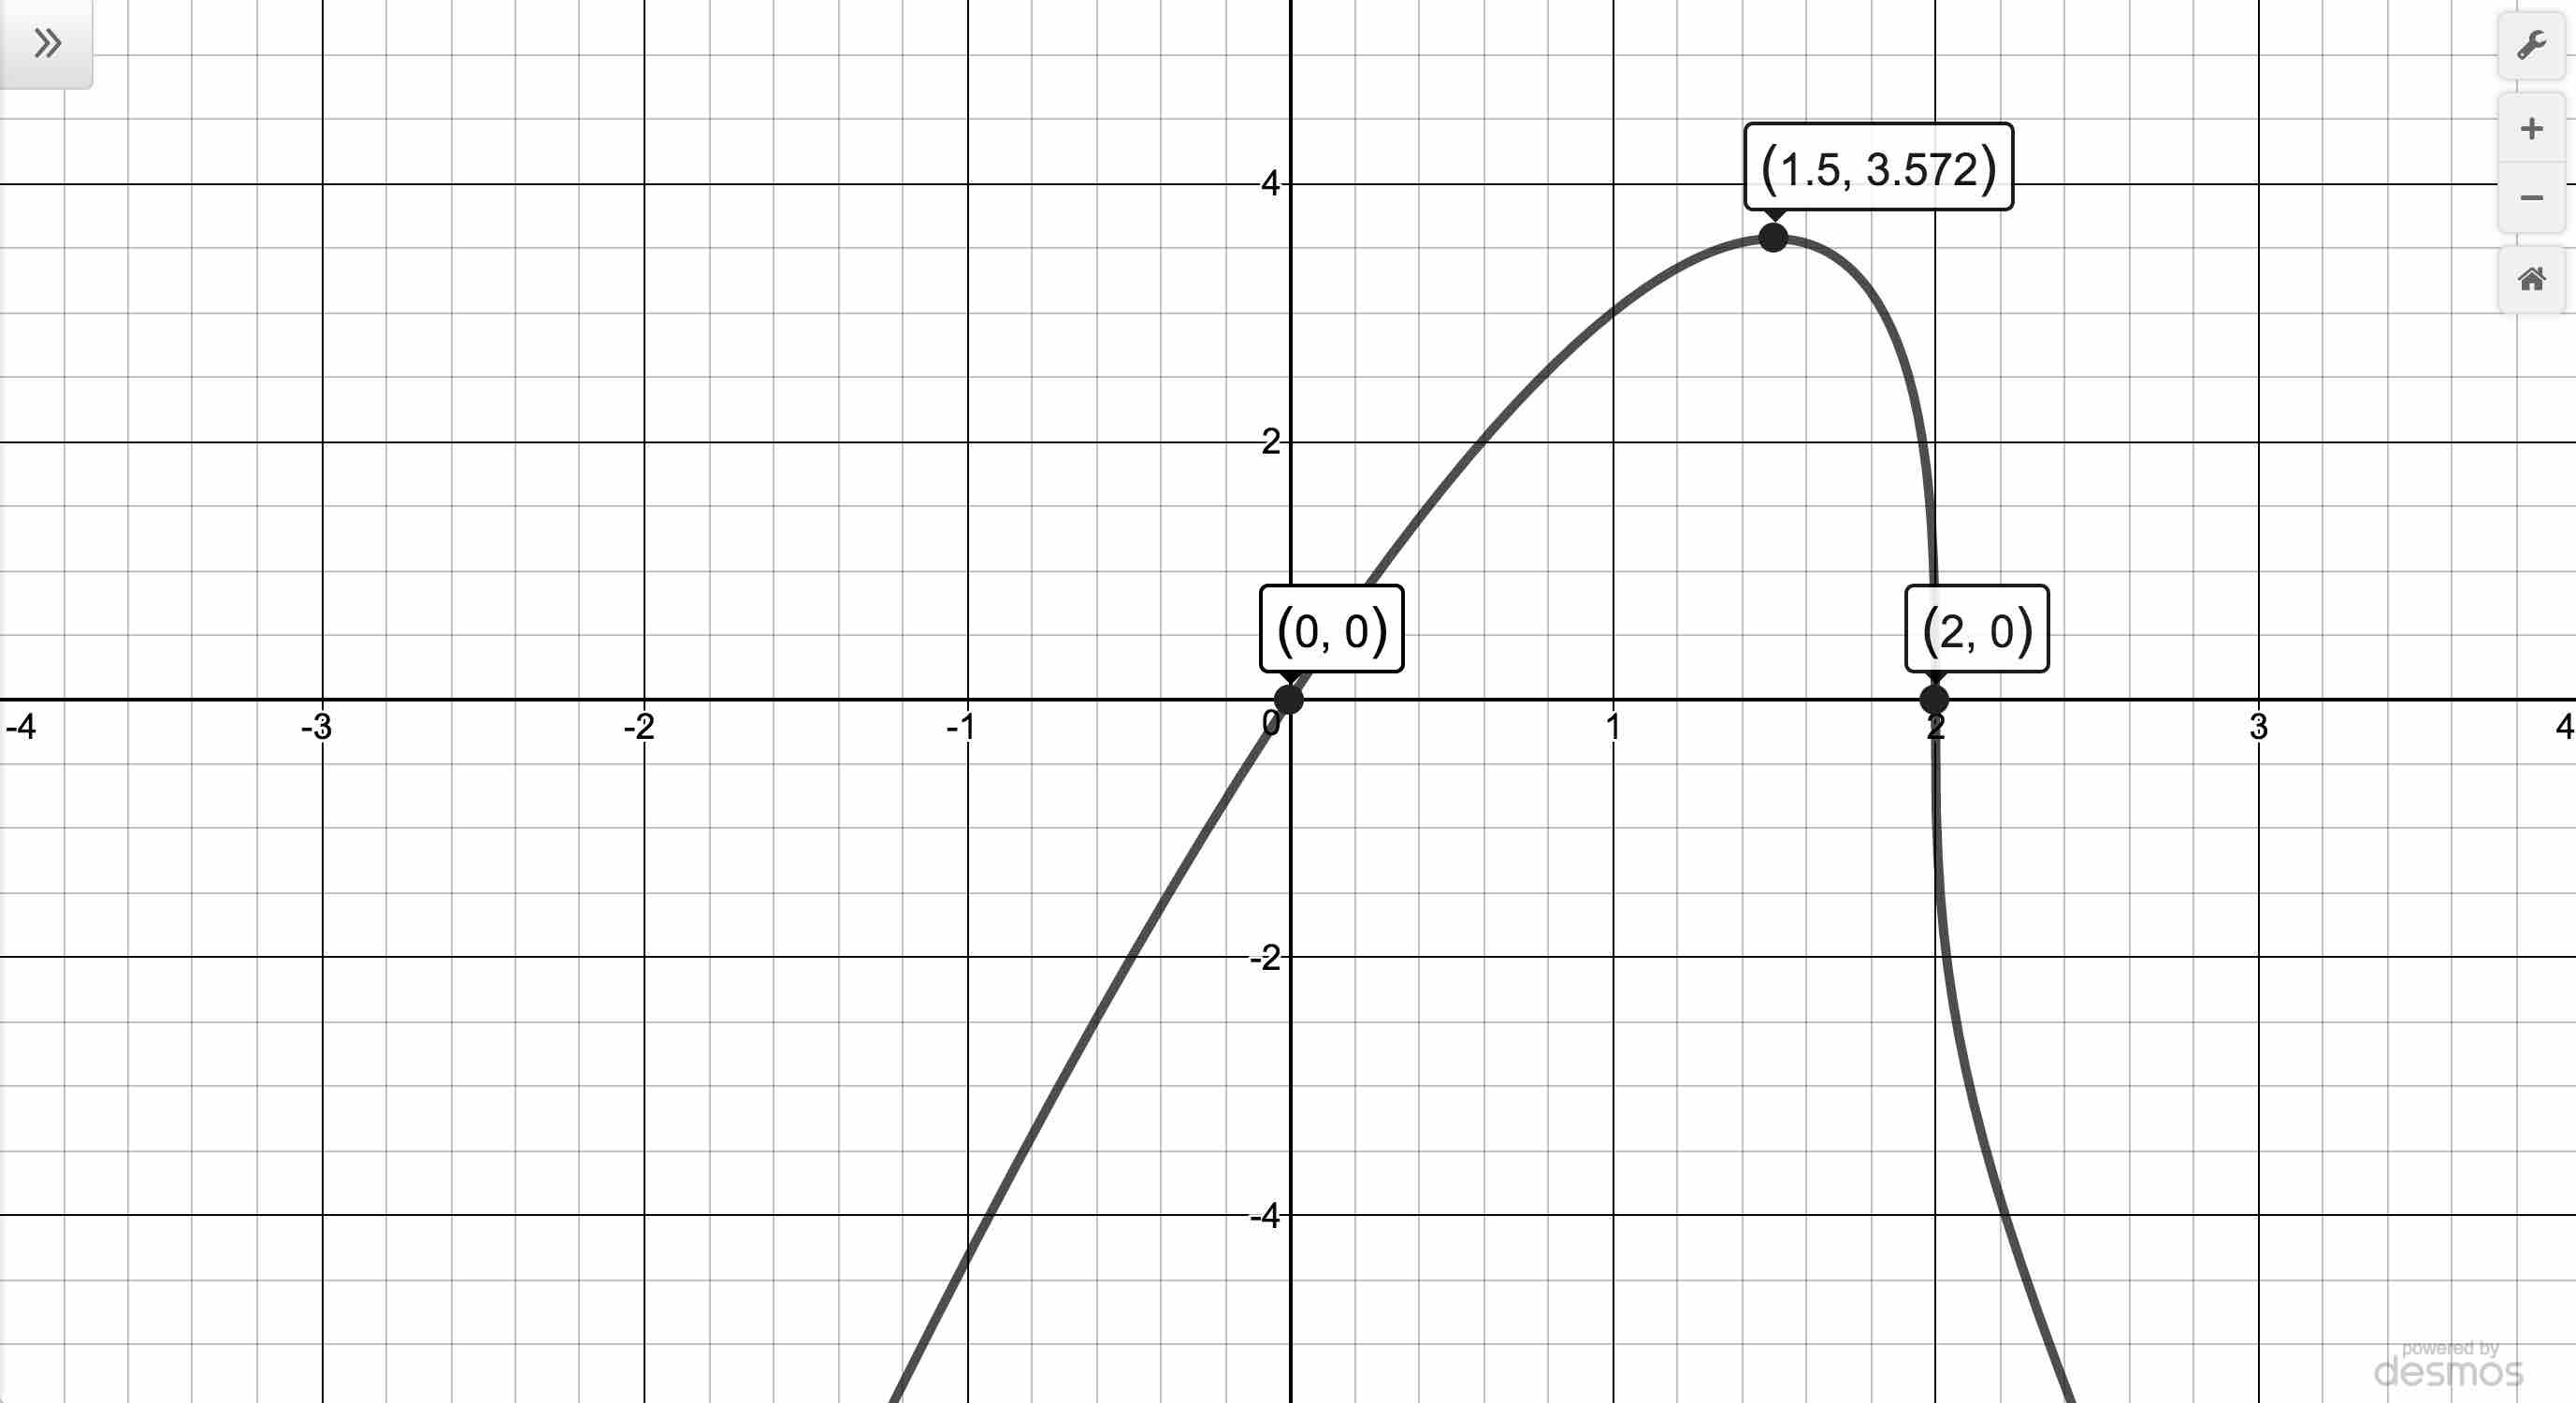
\includegraphics[width=3in]{./RootRadicalFunctionsGraphics/RadicalGraphEx01.jpg} &

\begin{mfpic}[20]{-4}{2}{-1}{1}
\arrow \reverse \arrow \polyline{(-4,0),(2,0)}
\xmarks{-2,0}
\tlabel[cc](-3, 0.5){$(-)$}
\tlabel[cc](-2,-0.5){$0$}
\tlabel[cc](-2,0.5){$0$}
\tlabel[cc](-1,0.5){$(+)$}
\tlabel[cc](0,-0.5){$2$}
\tlabel[cc](0,0.5){$0$}
\tlabel[cc](1,0.5){$(-)$}
\end{mfpic} \\

The graph of $y=f(x)$  \hspace{0.75in} & Sign Diagram for $f(x)$ \\


\end{tabular}
\end{center} 


\item  The index of the radical  in the expression for $g(t)$ is odd, so our only concern is the denominator.  Setting $t+1=0$ gives $t=-1$, which we exclude, so our domain is $\{ t \in \mathbb{R} \, | \, t \neq -1\}$ or using interval notation, $(-\infty, -1) \cup (-1, \infty)$.    

If we take the time to analyze the behavior of $g$ near $t=-1$, we find that as $t \rightarrow -1^{-}$, $g(t) = \sqrt[3]{\frac{8t}{t+1}}  \approx \sqrt[3]{\frac{-8}{\text{small $(-)$}}}  \approx \sqrt[3]{\text{ big$(+)$}} = \text{big $(+)$}$.  That is, $\ds{\lim_{t \rightarrow -1^{-}} g(t) = \infty}$.  Likewise, as $t \rightarrow -1^{+}$, $g(t)  \approx \sqrt[3]{\frac{-8}{\text{small $(+)$}}}  \approx \sqrt[3]{\text{ big $(-)$}} = \text{big $(-)$}$.  This suggests  $\ds{\lim_{t \rightarrow -1^{+}} g(t) = -\infty}$.  This behavior points to a vertical asymptote, $t=-1$.

To find the $t$-intercepts of the graph of $g$, we find the zeros of $g$ by setting $g(t) = \sqrt[3]{\frac{8t}{t+1}} = 0$.  Cubing both sides and clearing denominators  gives $8t = 0$ or $t = 0$.  Hence our  $t$-, and in this case,  $y$- intercept is $(0,0)$.

To determine the end behavior, we note that as $t \rightarrow  -\infty$ or $t \rightarrow  \infty$,  $\frac{8t}{t+1} \approx \frac{8t}{t} = 8$.  Since  $g(t) = \sqrt[3]{\frac{8t}{t+1}}$  it stands to reason that $\ds{\lim_{ t \rightarrow -\infty} g(t) =  \sqrt[3]{8} = 2}$ and, likewise, $\ds{\lim_{ t \rightarrow \infty} g(t) = 2}$  This suggests the graph of $y = g(t)$ has a horizontal asymptote at $y = 2$.

We graph $y = g(t)$ below on the left. The graph confirms our suspicions about the asymptotes $t = -1$ and $y = 2$.  Moreover, the range appears to be $(-\infty, 2) \cup (2, \infty)$.  

We could check if the graph ever crosses its horizontal asymptote by attempting to solve $g(t) =  \sqrt[3]{\frac{8t}{t+1}} = 2$.  Cubing both sides and clearing denominators gives $8t = 8(t+1)$ which gives $0 = 8$, a contradiction.  This proves $2$ is not in the range, as we had suspected. 

Scanning the graph,  there  appears to be no local extrema, and, moreover,  the graph suggests $g$  is increasing on $(-\infty, -1)$ and again on $(-1, \infty)$.  As with the previous example, the graph appears locally vertical near its intercept $(0,0)$.

\smallskip

To create a sign diagram for $g(t)$, we note that the function is undefined when $t = -1$ (so we place a `\textinterrobang' above it) and has a zero $t=0$.  When  $t<-1$, $g(t) > 0$ or $(+)$, for $-1<t<0$, $g(t)<0$ or $(-)$, and for $t>0$, $g(t) > 0$ or $(+)$.  Below on the right is a sign diagram for $g(t)$.

\begin{center}

\begin{tabular}{cc}

 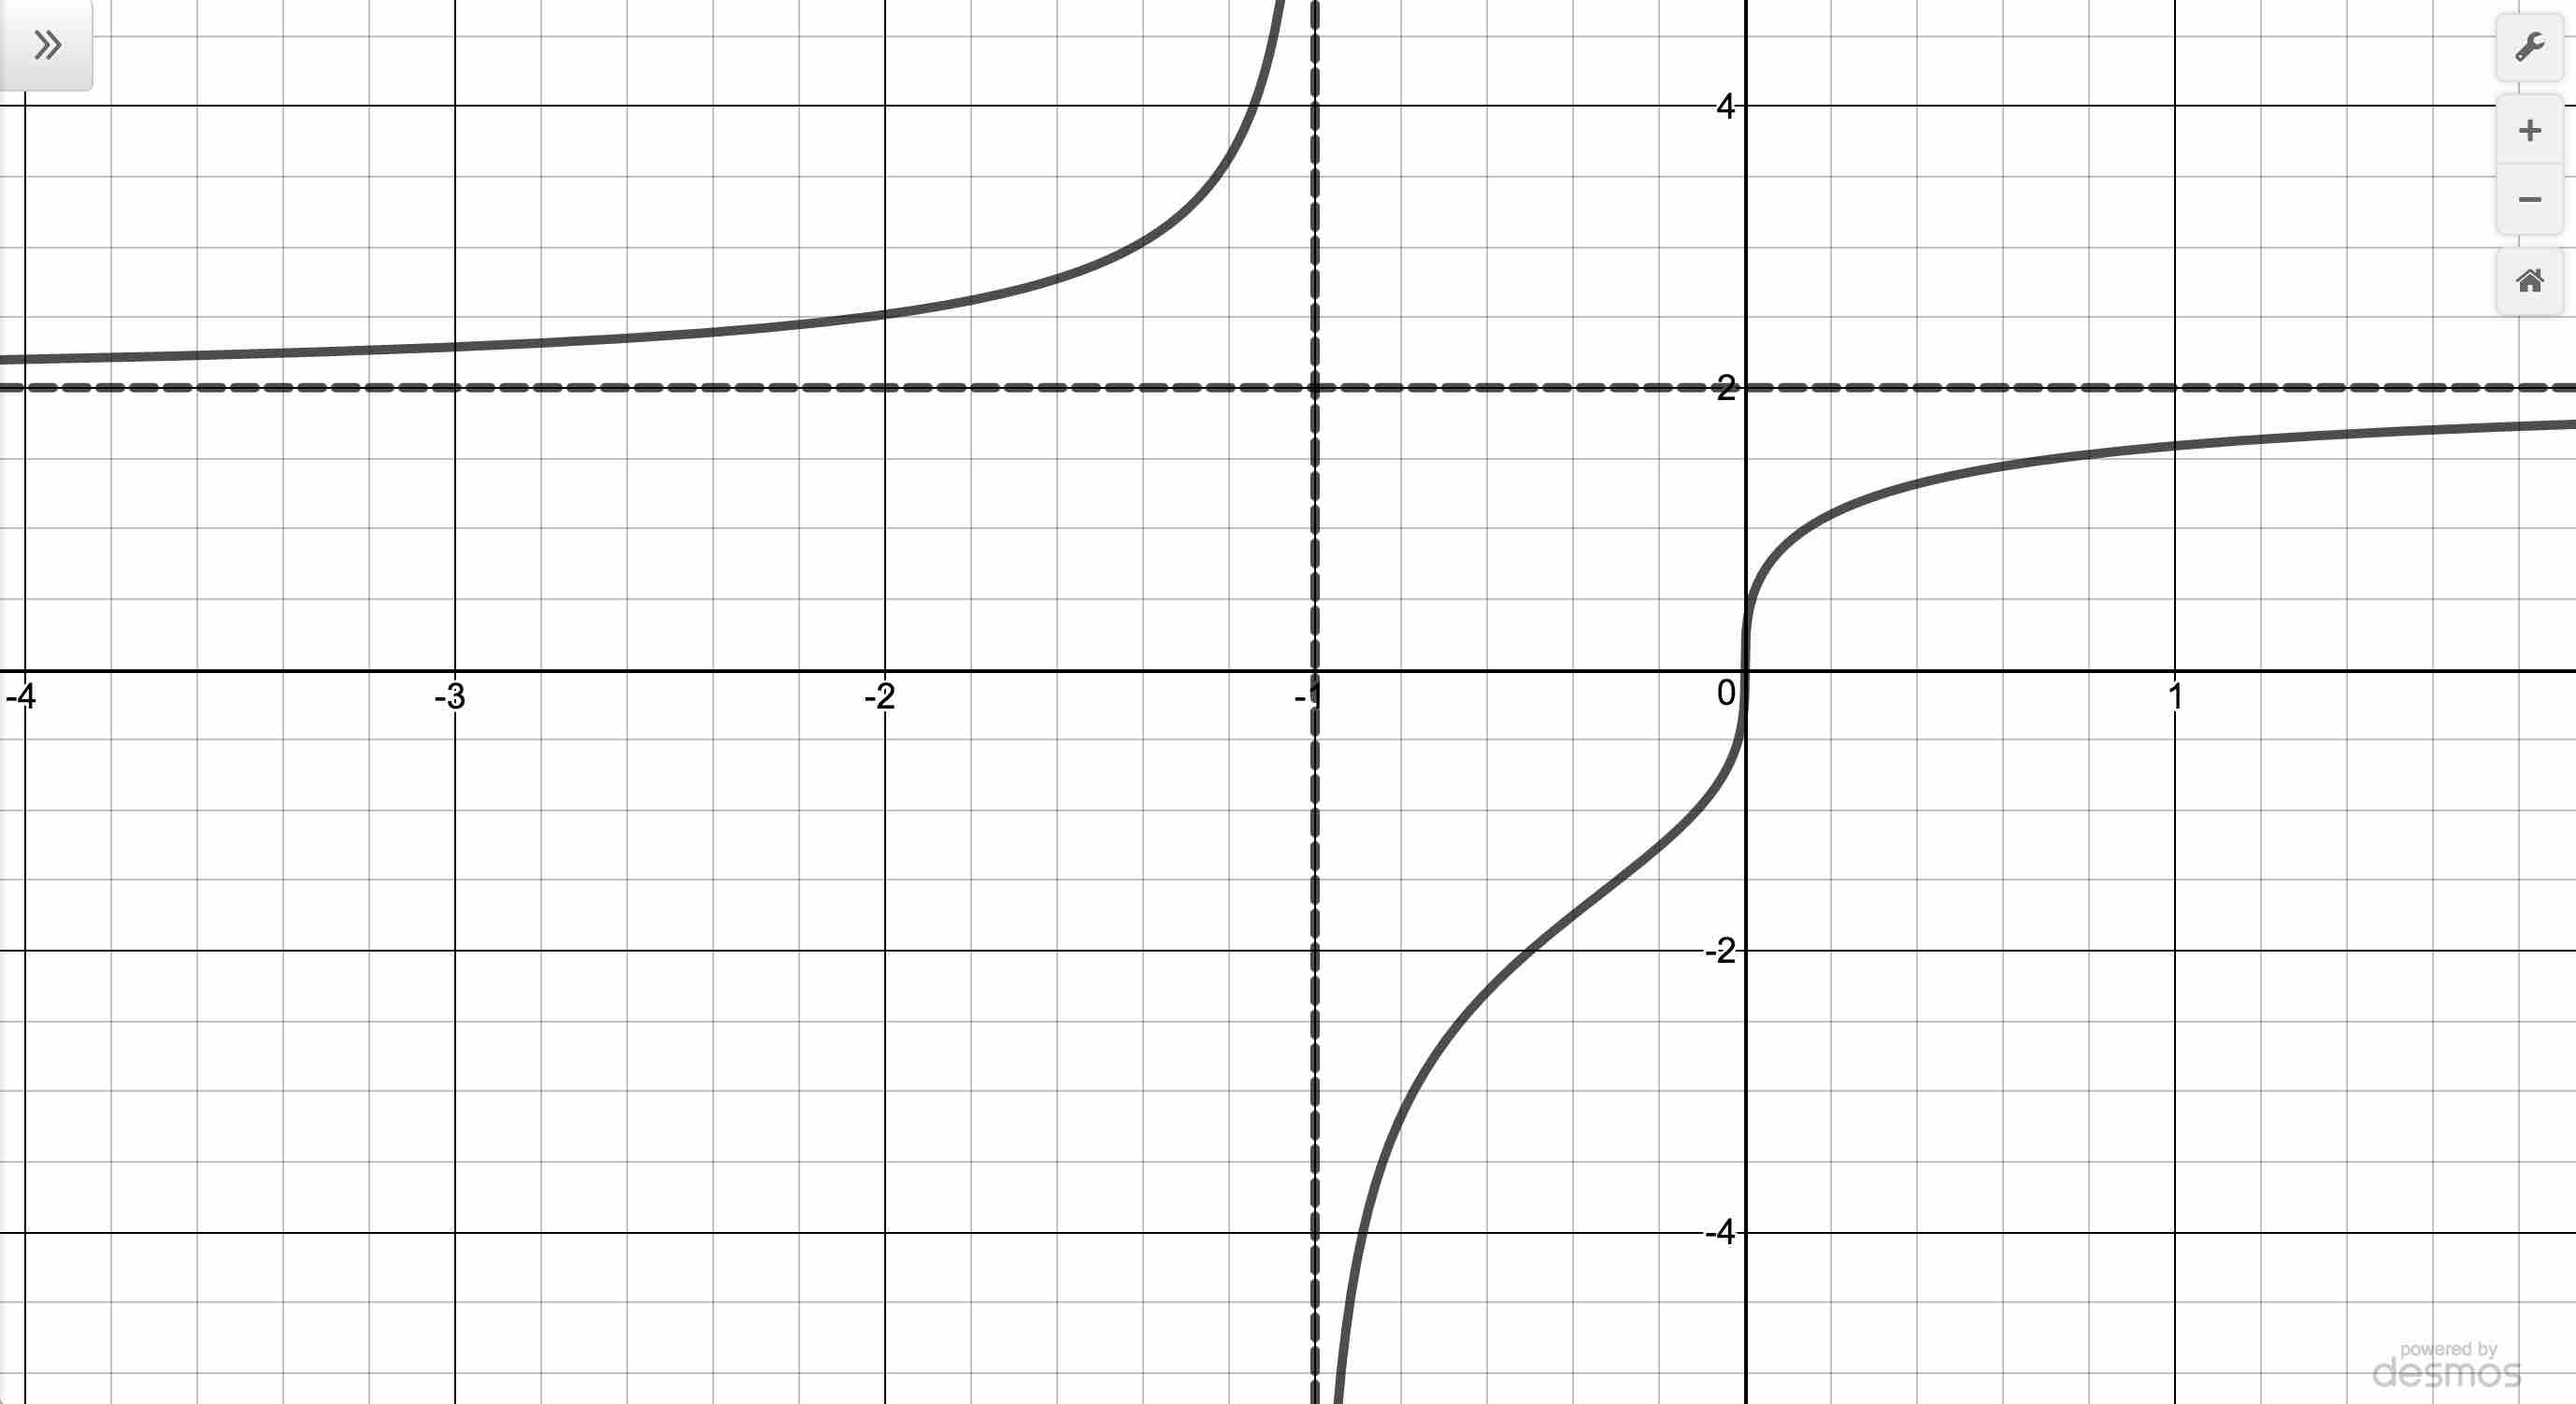
\includegraphics[width=3in]{./RootRadicalFunctionsGraphics/RadicalGraphEx02.jpg}  &
 
\begin{mfpic}[20]{-4}{2}{-1}{1}
\arrow \reverse \arrow \polyline{(-4,0),(2,0)}
\xmarks{-2,0}
\tlabel[cc](-3, 0.5){$(+)$}
\tlabel[cc](-2,-0.5){$-1 \hspace{7pt}$}
\tlabel[cc](-2,0.5){\textinterrobang}
\tlabel[cc](-1,0.5){$(-)$}
\tlabel[cc](0,-0.5){$0$}
\tlabel[cc](0,0.5){$0$}
\tlabel[cc](1,0.5){$(+)$}
\end{mfpic} \\

The graph of $y=g(t)$  \hspace{0.75in} & Sign Diagram for $g(t)$  \\


\end{tabular}
\end{center} 

 \item  The expression for $h(x) = \frac{3x}{\sqrt{x^2 + 1}}$ has both a denominator and an even-indexed radical, so we have to be extra cautious here.  Fortunately for us, the quantity $x^2+1 >0$ for all real numbers $x$. Not only does this mean $\sqrt{x^2+1}$ is always defined, it also tells us $\sqrt{x^2+1}>0$ for all $x$, too.  This means the domain of $h$ is all real numbers, $(-\infty, \infty)$.
 
Solving for the zeros of $h$ gives only $x = 0$, and we find, once again, $(0,0)$ is both our lone $x$- and $y$-intercept.  

Moving on to end behavior, as $x \rightarrow -\infty$ or  $x \rightarrow \infty$, the term $x^2$ is the dominant term in the radicand in the denominator. As such, $h(x) = \frac{3x}{\sqrt{x^2 + 1}} \approx \frac{3x}{\sqrt{x^2}} = \frac{3x}{|x|}$.  As $x \rightarrow -\infty$, $|x| = -x$ (since $x<0$) and hence, $h(x)\approx  \frac{3x}{-x} = -3$, so $\ds{\lim_{x \rightarrow -\infty} h(x) =  -3}$.   As $x \rightarrow \infty$, $|x| = x$ (since $x>0$), so $h(x) \approx \frac{3x}{x} = 3$, so $\ds{\lim_{x \rightarrow \infty} h(x) =  3}$. 
 
  This analysis suggests the graph of $y=h(x)$ has not one, but \textit{two} horizontal asymptotes.\footnote{We warned you this was coming \ldots see the discussion following Theorem \ref{hathm} in Section \ref{IntroRational}.} The graph of $h$ below on the left bears this out.

From the graph, we see the range of $h$ appears to be $(-3,3)$.  Attempting to solve $h(x) = \frac{3x}{\sqrt{x^2 + 1}} = -3$ or  $h(x) = \frac{3x}{\sqrt{x^2 + 1}} = 3$ gives, in either case, $9x^2 = 9(x^2+1)$ which reduces to $0 = 9$, a contradiction.  Hence, the graph of $y = h(x)$ never reaches its horizontal asymptotes. Moreover, $h$ appears to be always increasing, with no local extrema or `unusual' steepness.  One last remark:  it appears as if the graph of $h$ is symmetric about the origin.  We check $h(-x) = \frac{3(-x)}{\sqrt{(-x)^2+1}} = - \frac{3x}{\sqrt{x^2 + 1}} = -h(x)$ which verifies $h$ is odd.

\smallskip

Since the domain of $h$ is all real number and the only zero of $h$ is $x=0$, the sign diagram for $h(x)$ is fairly straight forward.  For $x<0$, $h(x)<0$ or $(-)$ and for $x>0$, $h(x) >0$ or $(+)$.  The sign diagram for $h(x)$ is below on the right.

\begin{center}

\begin{tabular}{cc}

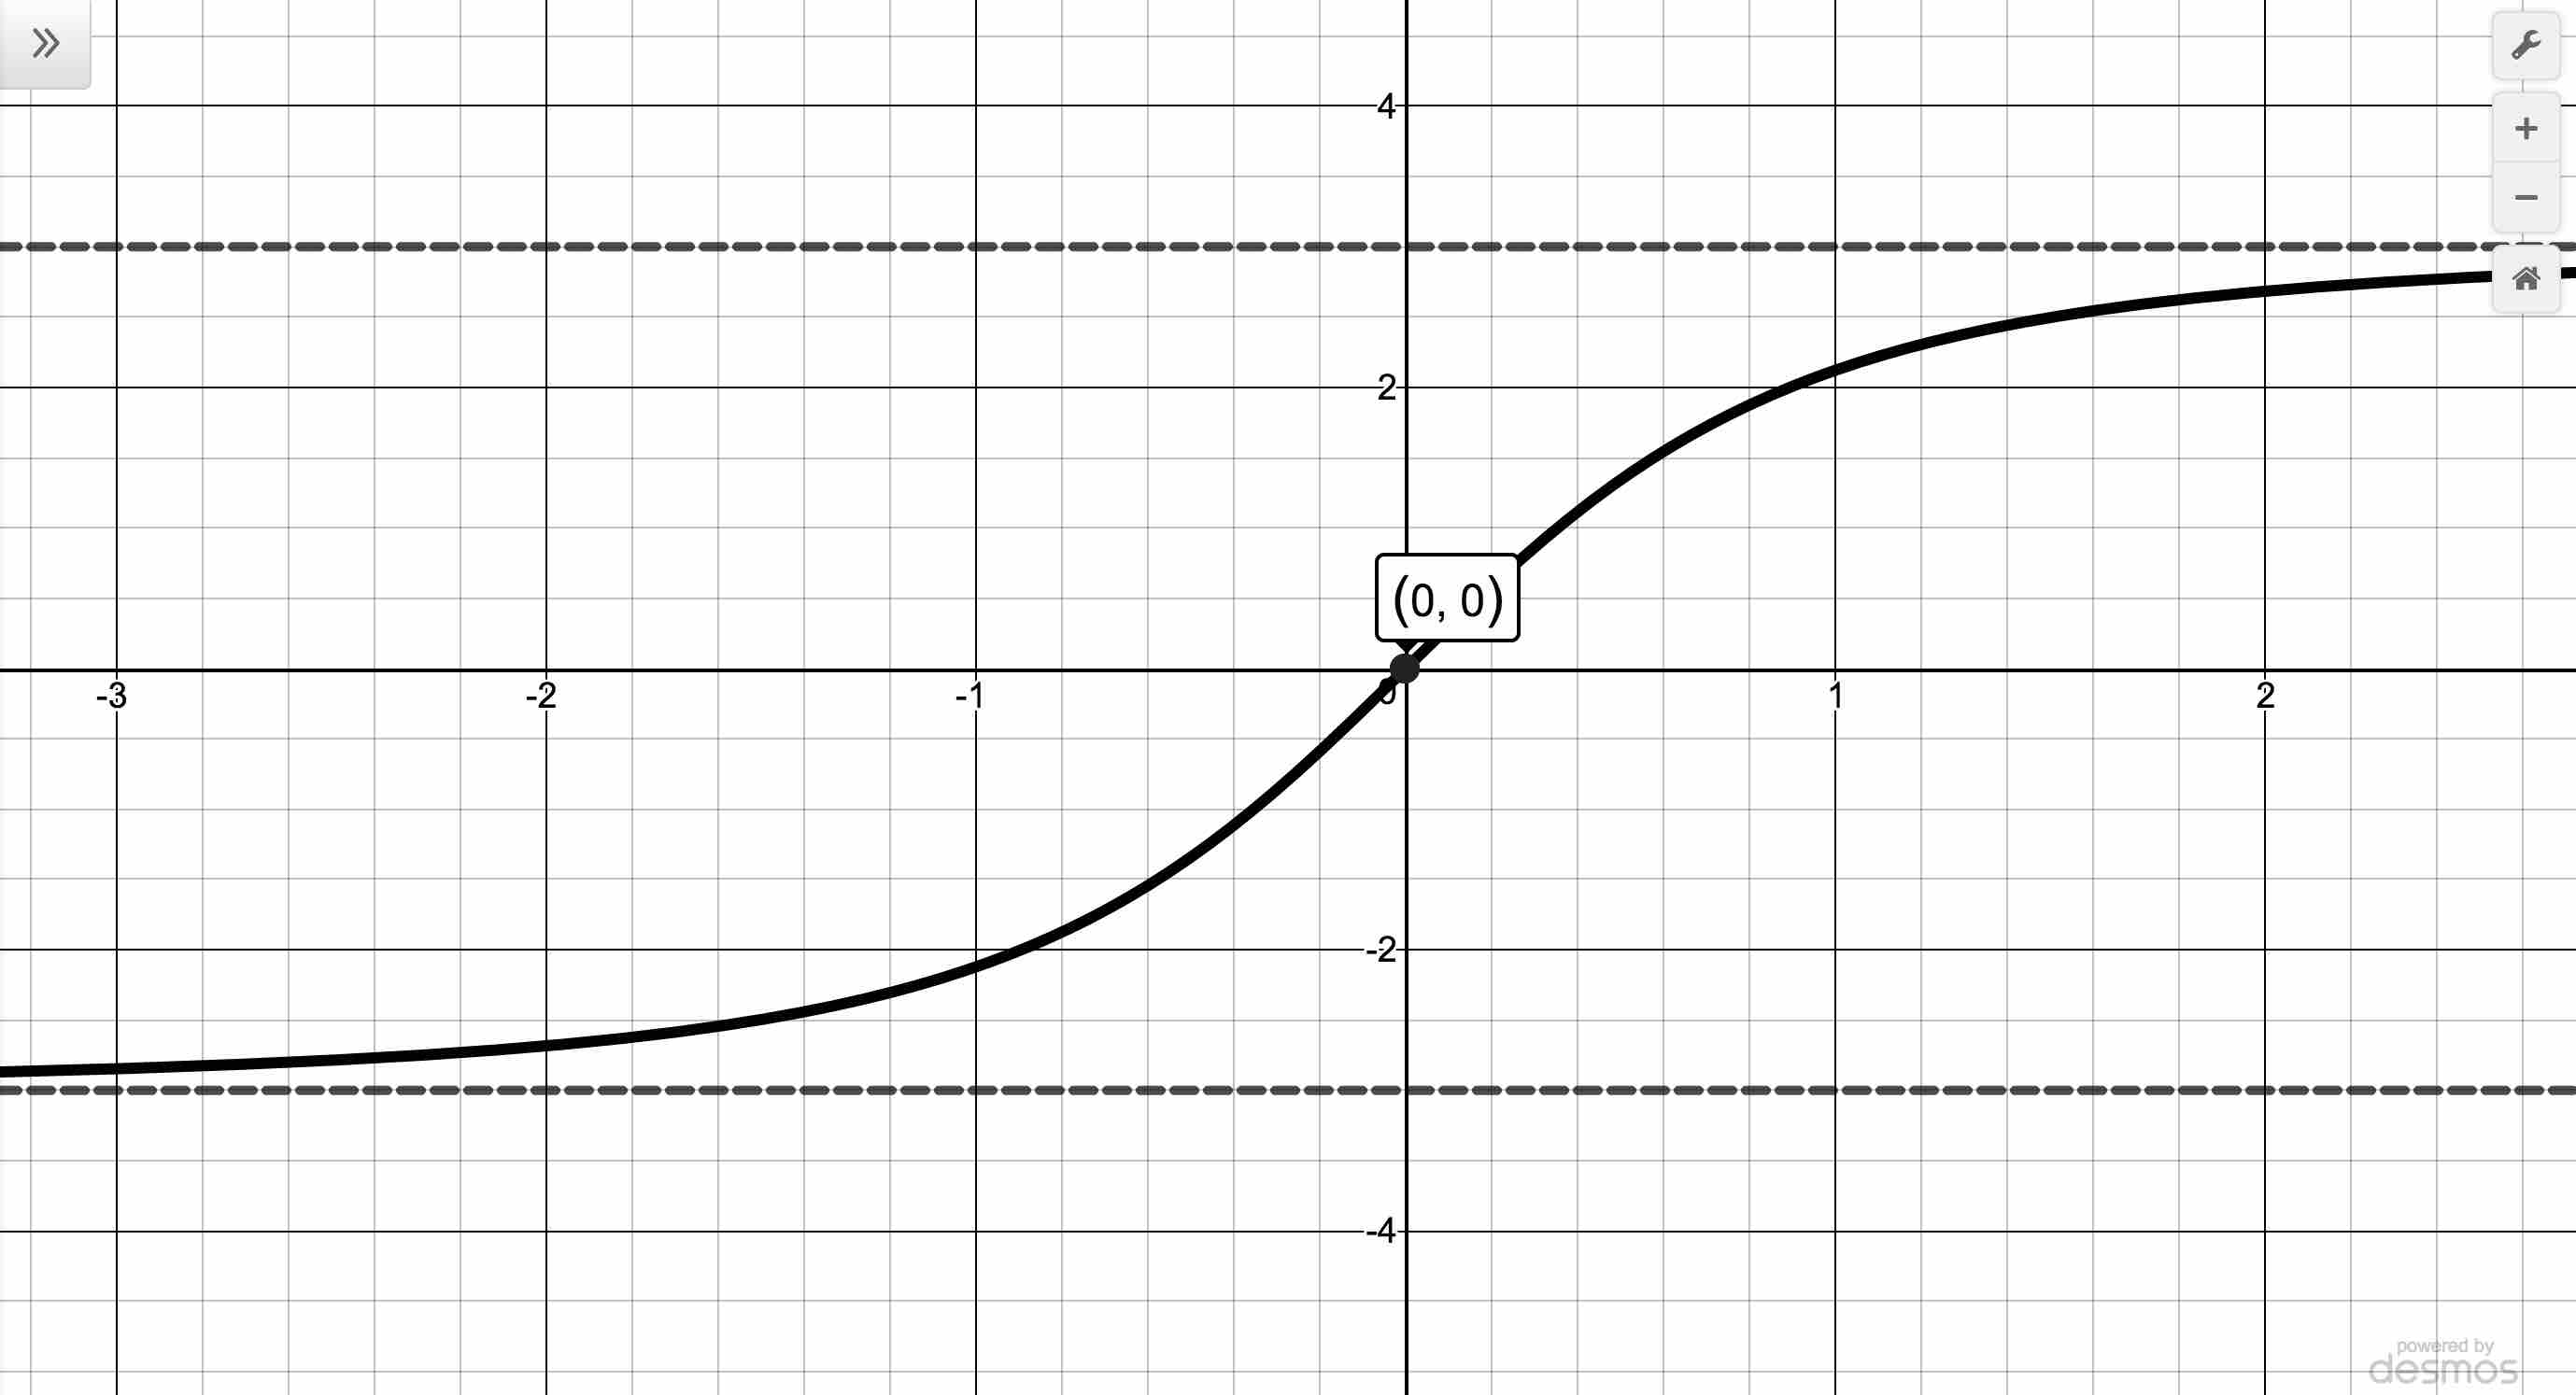
\includegraphics[width=3in]{./RootRadicalFunctionsGraphics/RadicalGraphEx03.jpg} &

\begin{mfpic}[20]{-4}{2}{-1}{1}
\arrow \reverse \arrow \polyline{(-2,0),(2,0)}
\xmarks{0}
\tlabel[cc](-1,0.5){$(-)$}
\tlabel[cc](0,-0.5){$0$}
\tlabel[cc](0,0.5){$0$}
\tlabel[cc](1,0.5){$(+)$}
\end{mfpic} \\

The graph of $y=h(x)$  \hspace{0.75in} & Sign Diagram for $h(x)$ \\


\end{tabular}
\end{center} 



\item  The first thing to note about the expression  $r(t) = t^{-1} \sqrt{16t^4-1}$ is that $t^{-1} = \frac{1}{t}$.  Hence, we must exclude $t=0$ from the domain straight away. Next, we have an even-indexed radical expression: $\sqrt{16t^4-1}$.  In order for this to return a real number, we require  $16t^4-1 \geq 0$.  Instead of using a sign diagram to solve this,\footnote{See Section \ref{RealZeros}} we opt instead to  \textit{carefully} use properties of radicals.  Isolating $t^4$, we have $t^4 \geq \frac{1}{16}$.  Since the root functions are increasing, we can apply the fourth root to both sides and preserve the inequality:  $\sqrt[4]{t^4} \geq \sqrt[4]{\frac{1}{16}}$ which gives\footnote{Recall: $\sqrt[n]{x^n} = |x|$, not $x$,  if $n$ is even.} $|t| \geq \frac{1}{2}$. Note that since $t =0$ does \textit{not} satisfy this inequality, restricting $t$ in this manner takes care of  \textit{both} domain issues, so the domain is  $\left(-\infty, -\frac{1}{2} \right] \cup \left[\frac{1}{2}, \infty \right)$.   

Next, we look for zeros.  Setting $r(t) = t^{-1} \sqrt{16t^4-1} = \frac{\sqrt{16t^4-1}}{t}=0$ gives $\sqrt{16t^4-1} = 0$.  After squaring both sides, we get $16t^4-1 = 0$ or $t^4 = \frac{1}{16}$.  Extracting fourth roots, we get $t = \pm \frac{1}{2}$. Both of these are (barely!) in the domain of $r$, so our $t$ intercepts are $\left( -\frac{1}{2}, 0\right)$ and $\left( \frac{1}{2}, 0\right)$.  Note, the graph of $r$ has no $y$-intercept, since $r(0)$ is undefined ($t=0$ is not in the domain of $r$).  

Concerning end behavior, we note the term $16t^4$ dominates the radicand $\sqrt{16t^4-1}$ as $t \rightarrow - \infty$ or $t \rightarrow \infty$ ,  hence, $r(t) = \frac{\sqrt{16t^4-1}}{t} \approx \frac{\sqrt{16t^4}}{t} = \frac{4t^2}{t} = 4t$.  This suggests the graph of $y = r(t)$ has a slant asymptote with slope $4$.\footnote{Note: this analysis suggests the slant asymptote is $y = 4t+b$, but from this analysis, we cannot determine the value of $b$.  As with slant asymptotes in Section \ref{IntroRational}, we'd need to perform a more detailed analysis which we omit in this case owing to the complexity of the function. (You'll have the tools in Calculus, however!)}  At this point, we can at least write $\ds{\lim_{t \rightarrow -\infty} r(t) = -\infty}$. and $\ds{\lim_{t \rightarrow \infty} r(t) = \infty}$.

We graph $y=r(t)$ below on the left.  We see the range appears to be all real numbers, $(-\infty, \infty)$.  It appears as if $r$ is increasing on $\left(-\infty, -\frac{1}{2} \right]$ and again on $\left[\frac{1}{2}, \infty \right)$.  The graph does appear to be asymptotic to $y = 4t$, and it also appears to be symmetric about the origin.  Sure enough, we find  $r(-t) = \frac{\sqrt{16(-t)^4-1}}{-t}  = - \frac{\sqrt{16t^4-1}}{t} = -r(t)$, proving $r$ is an odd function.

\smallskip

To construct the sign diagram for $r(t)$ we note $r$ has two zeros, $t = \pm \frac{1}{2}$.  For $t < \frac{1}{2}$, $r(t) < 0$ or $(-)$ and when $t > \frac{1}{2}$, $r(t) > 0$ or $(+)$.  When $-\frac{1}{2} < t < \frac{1}{2}$, $r$ is undefined so we have removed that segment from the diagram, as seen below on the right.

\begin{center}

\begin{tabular}{cc}

 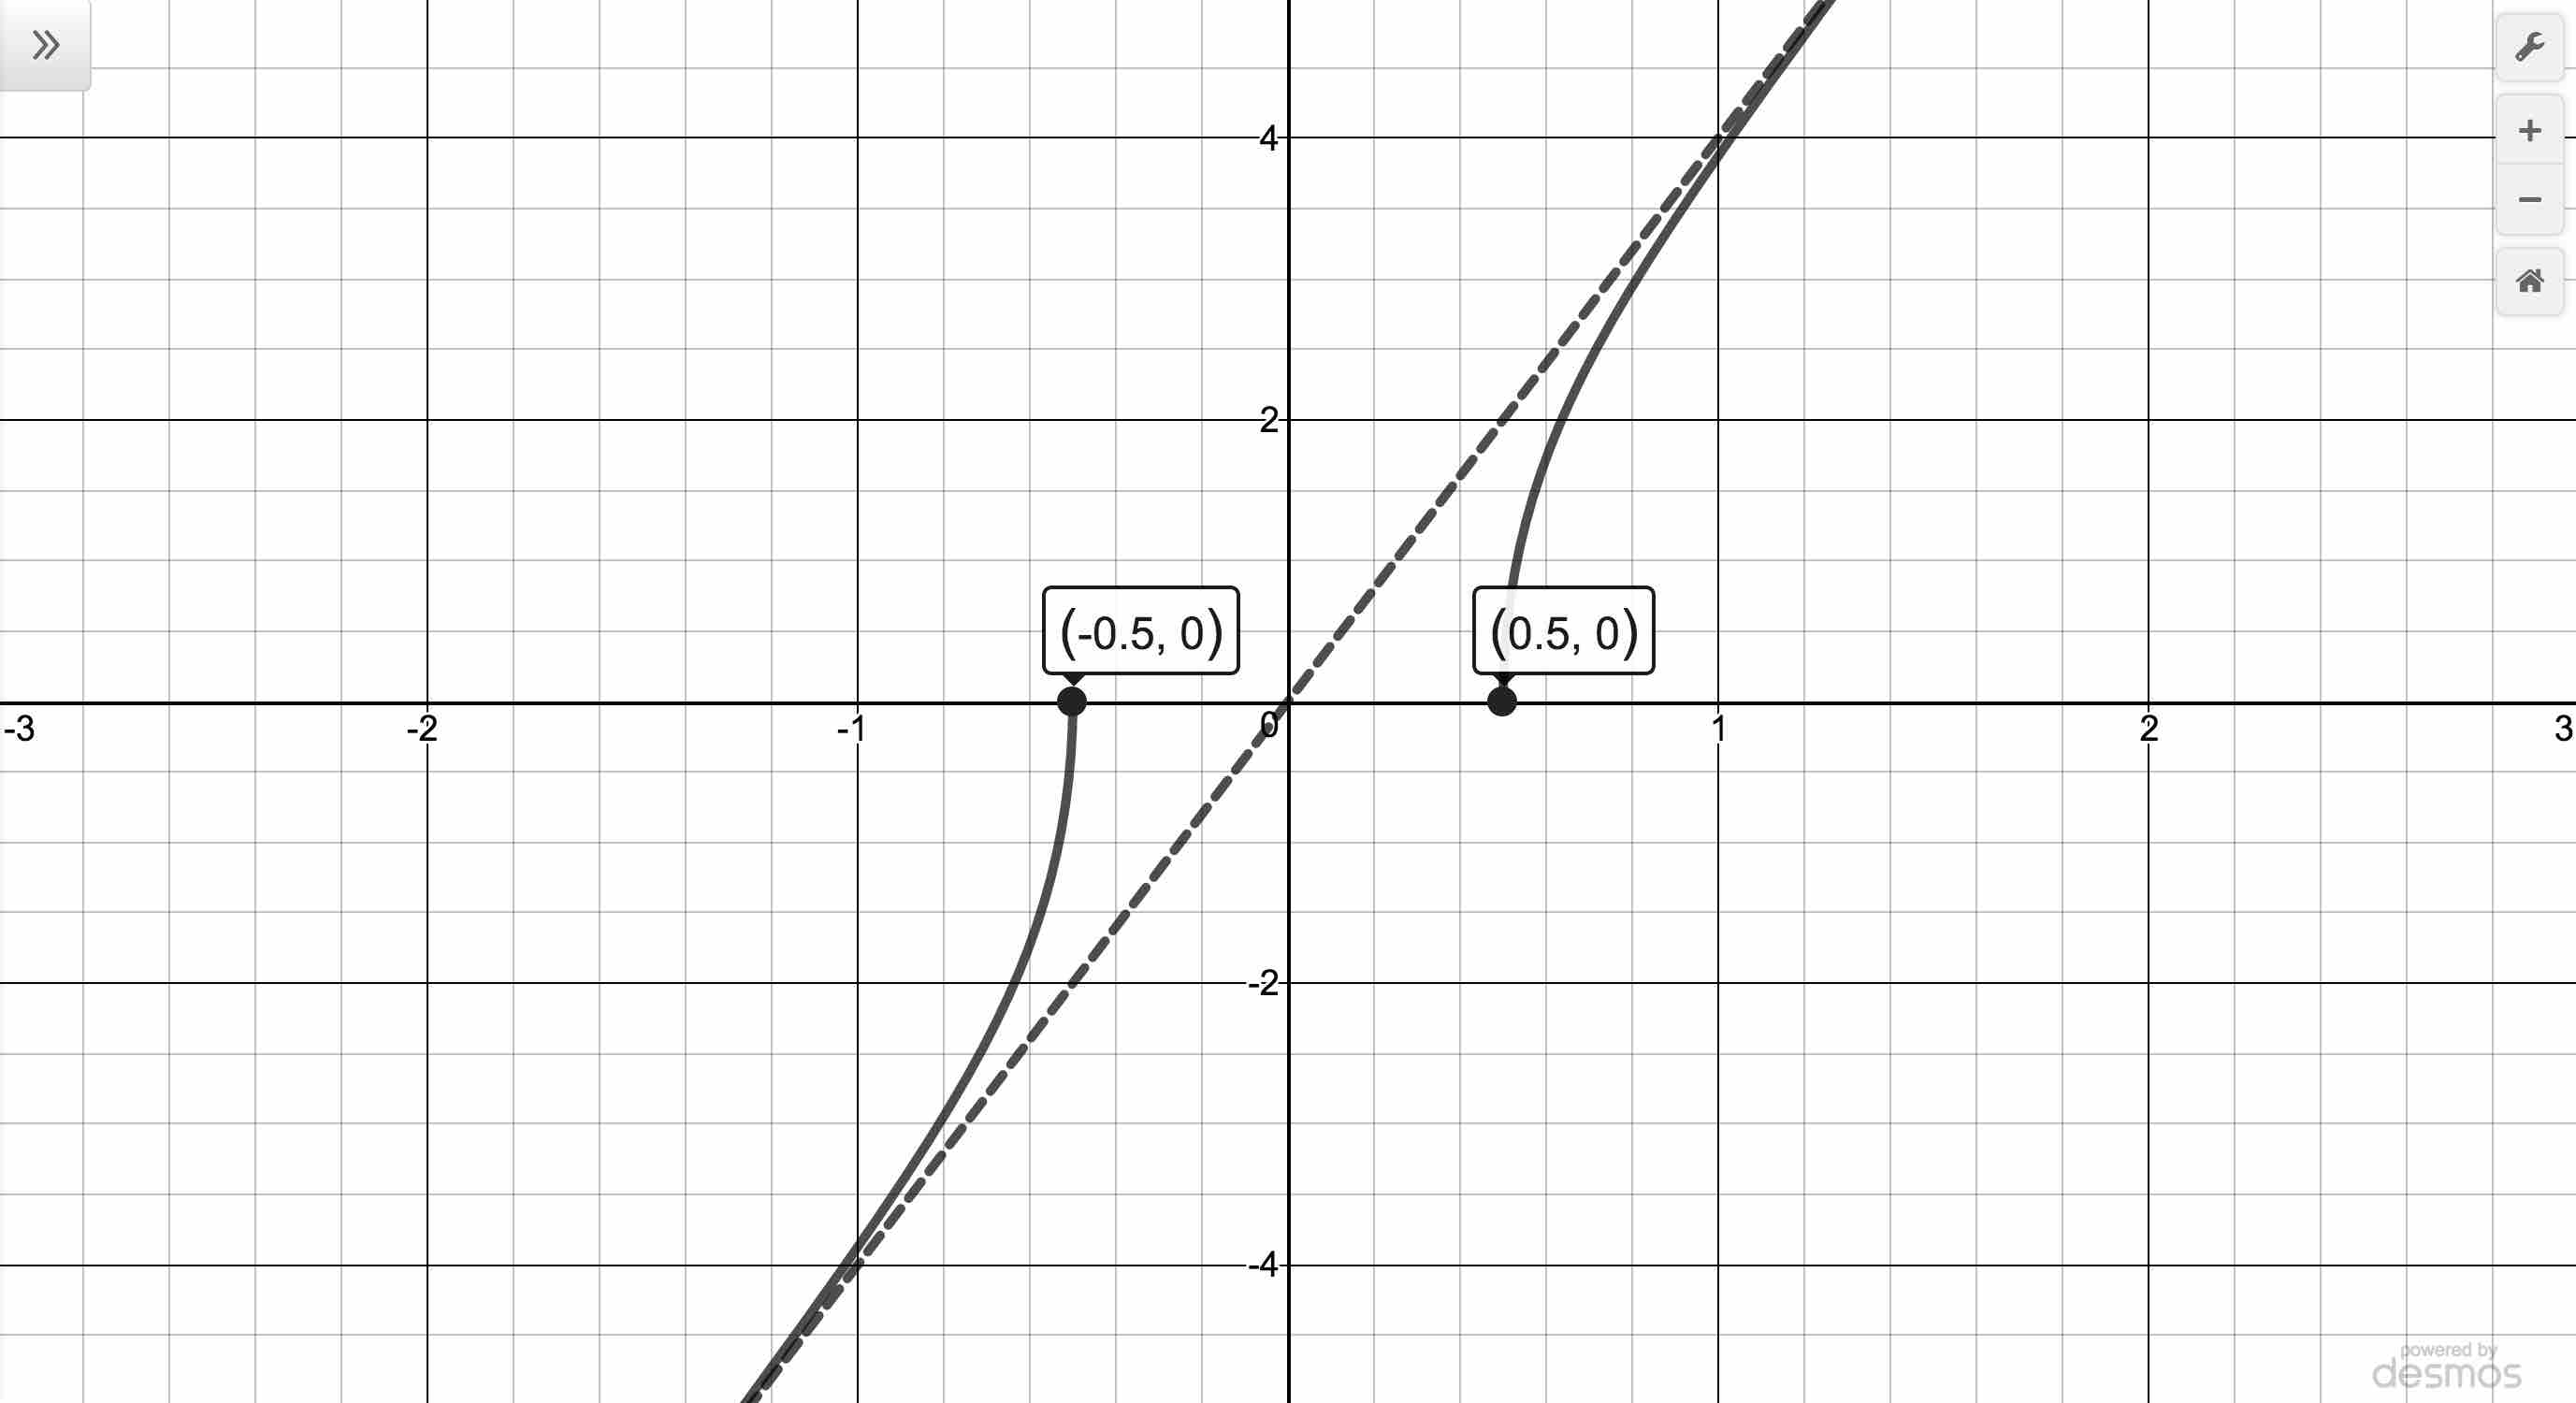
\includegraphics[width=3in]{./RootRadicalFunctionsGraphics/RadicalGraphEx04.jpg} &
  
 \begin{mfpic}[20][10]{0}{4}{-1.5}{1.5}
\arrow \polyline{(2,0), (0,0)}
\arrow \polyline{(3,0), (5,0)}
\xmarks{2,3}
\tlabel[cc](2,-1){$-\frac{1}{2} \hspace{7pt}$}
\tlabel[cc](1,1){$(-)$}
\tlabel[cc](4,1){$(+)$}
\tlabel[cc](2,1){$0$}
\tlabel[cc](3,1){$0$}
\tlabel[cc](3,-1){$\frac{1}{2}$}
\end{mfpic}
\\

The graph of $y=r(t)$  \hspace{0.75in} & Sign Diagram for $r(t)$. \\


\end{tabular}
\end{center} 



\qed
\end{enumerate}

\end{ex}

We end this section with a classic application of root functions.


\begin{ex} \label{SasquatchCable} Carl wishes to get high speed internet service installed in his remote Sasquatch observation post located $30$ miles from Route $117$. The nearest junction box is located $50$ miles down the road from the post, as indicated in the diagram below.  Suppose it costs $\$ 15$ per mile to run cable along the road and $\$ 20$ per mile to run cable off of the road.

\begin{enumerate}

\item   Find an expression $C(x)$ which computes the cost of connecting the Junction Box to the Outpost as a function of $x$, the number of miles the cable is run along Route $117$ before heading off road directly towards the Outpost.  Determine a reasonable applied domain for the problem.

\item  Use your calculator to graph $y=C(x)$ on its domain.  What is the minimum cost?  How far along Route $117$ should the cable be run before turning off of the road?

\end{enumerate}

\begin{center}
\begin{mfpic}[12]{-1}{15}{-1}{9}

\xmarks{0, 4}

\arrow \reverse \arrow \polyline{(0,8.75),(0,0.25)}

\arrow \reverse \arrow \polyline{(0.25,0),(3.75,0)}

\arrow \reverse \arrow \polyline{(4.25,0),(9.75,0)}

\arrow \reverse \arrow \polyline{(0,-1),(10,-1)}

\dashed \polyline{(4,0),(0,9)}

\point[3pt]{(0,9), (10,0)}

\tlabel[cc](1.25,9){\scriptsize Outpost}

\tlabel[cc](12,0){\scriptsize Junction Box}

\tlabel[cc](7,0.5){$x$}

\tlabel[cc](2,0.5){$y$}

\tlabel[cc](3,4.5){$z$}

\tlabel[cc](5,-.5){\scriptsize Route $117$}

\tlabel[cc](5,-2){\scriptsize $50$ miles}

\tlabel[cc](-0.5,0){\rotatebox{90}{\hspace{1.5in} \scriptsize $30$ miles}}

\end{mfpic}
\end{center}



{\bf Solution.}

\begin{enumerate}

\item  The cost is broken into two parts:  the cost to run cable along Route $117$ at $\$15$ per mile, and the cost to run it off road at $\$20$ per mile.  Since $x$ represents the miles of cable run along Route $117$, the cost  for that portion is $15x$.  
From the diagram, we see that the number of miles the cable is run off road is $z$, so the cost of that portion is $20z$.  Hence, the total cost is $15x + 20z$.  

\smallskip

Our next goal is to determine $z$ in terms of $x$.  The diagram suggests we can use the Pythagorean Theorem to get $y^2+30^2 = z^2$.  But we also see $x+y = 50$ so that $y=50-x$.  Substituting $(50-x)$ in for $y$ we obtain $z^2 = (50-x)^2+900$.  Solving for $z$, we obtain $z = \pm \sqrt{(50-x)^2+900}$.  Since $z$ represents a distance, we choose $z = \sqrt{(50-x)^2+900}$.

Hence, the cost as a function of $x$  is given by $C(x) = 15x + 20\sqrt{(50-x)^2+900}$.  From the context of the problem, we have $0 \leq x \leq 50$.

\item  We graph $y=C(x)$ below and find our (local) minimum to be at the point $(15.98, 1146.86)$.  Here the $x$-coordinate tells us that in order to minimize cost, we should run $15.98$ miles of cable along Route 117 and then turn off of the road and head towards the outpost. The $y$-coordinate tells us that the minimum cost, in dollars, to do so is $\$1146.86$.  The ability to stream live SasquatchCasts?  Priceless.

\medskip

\centerline{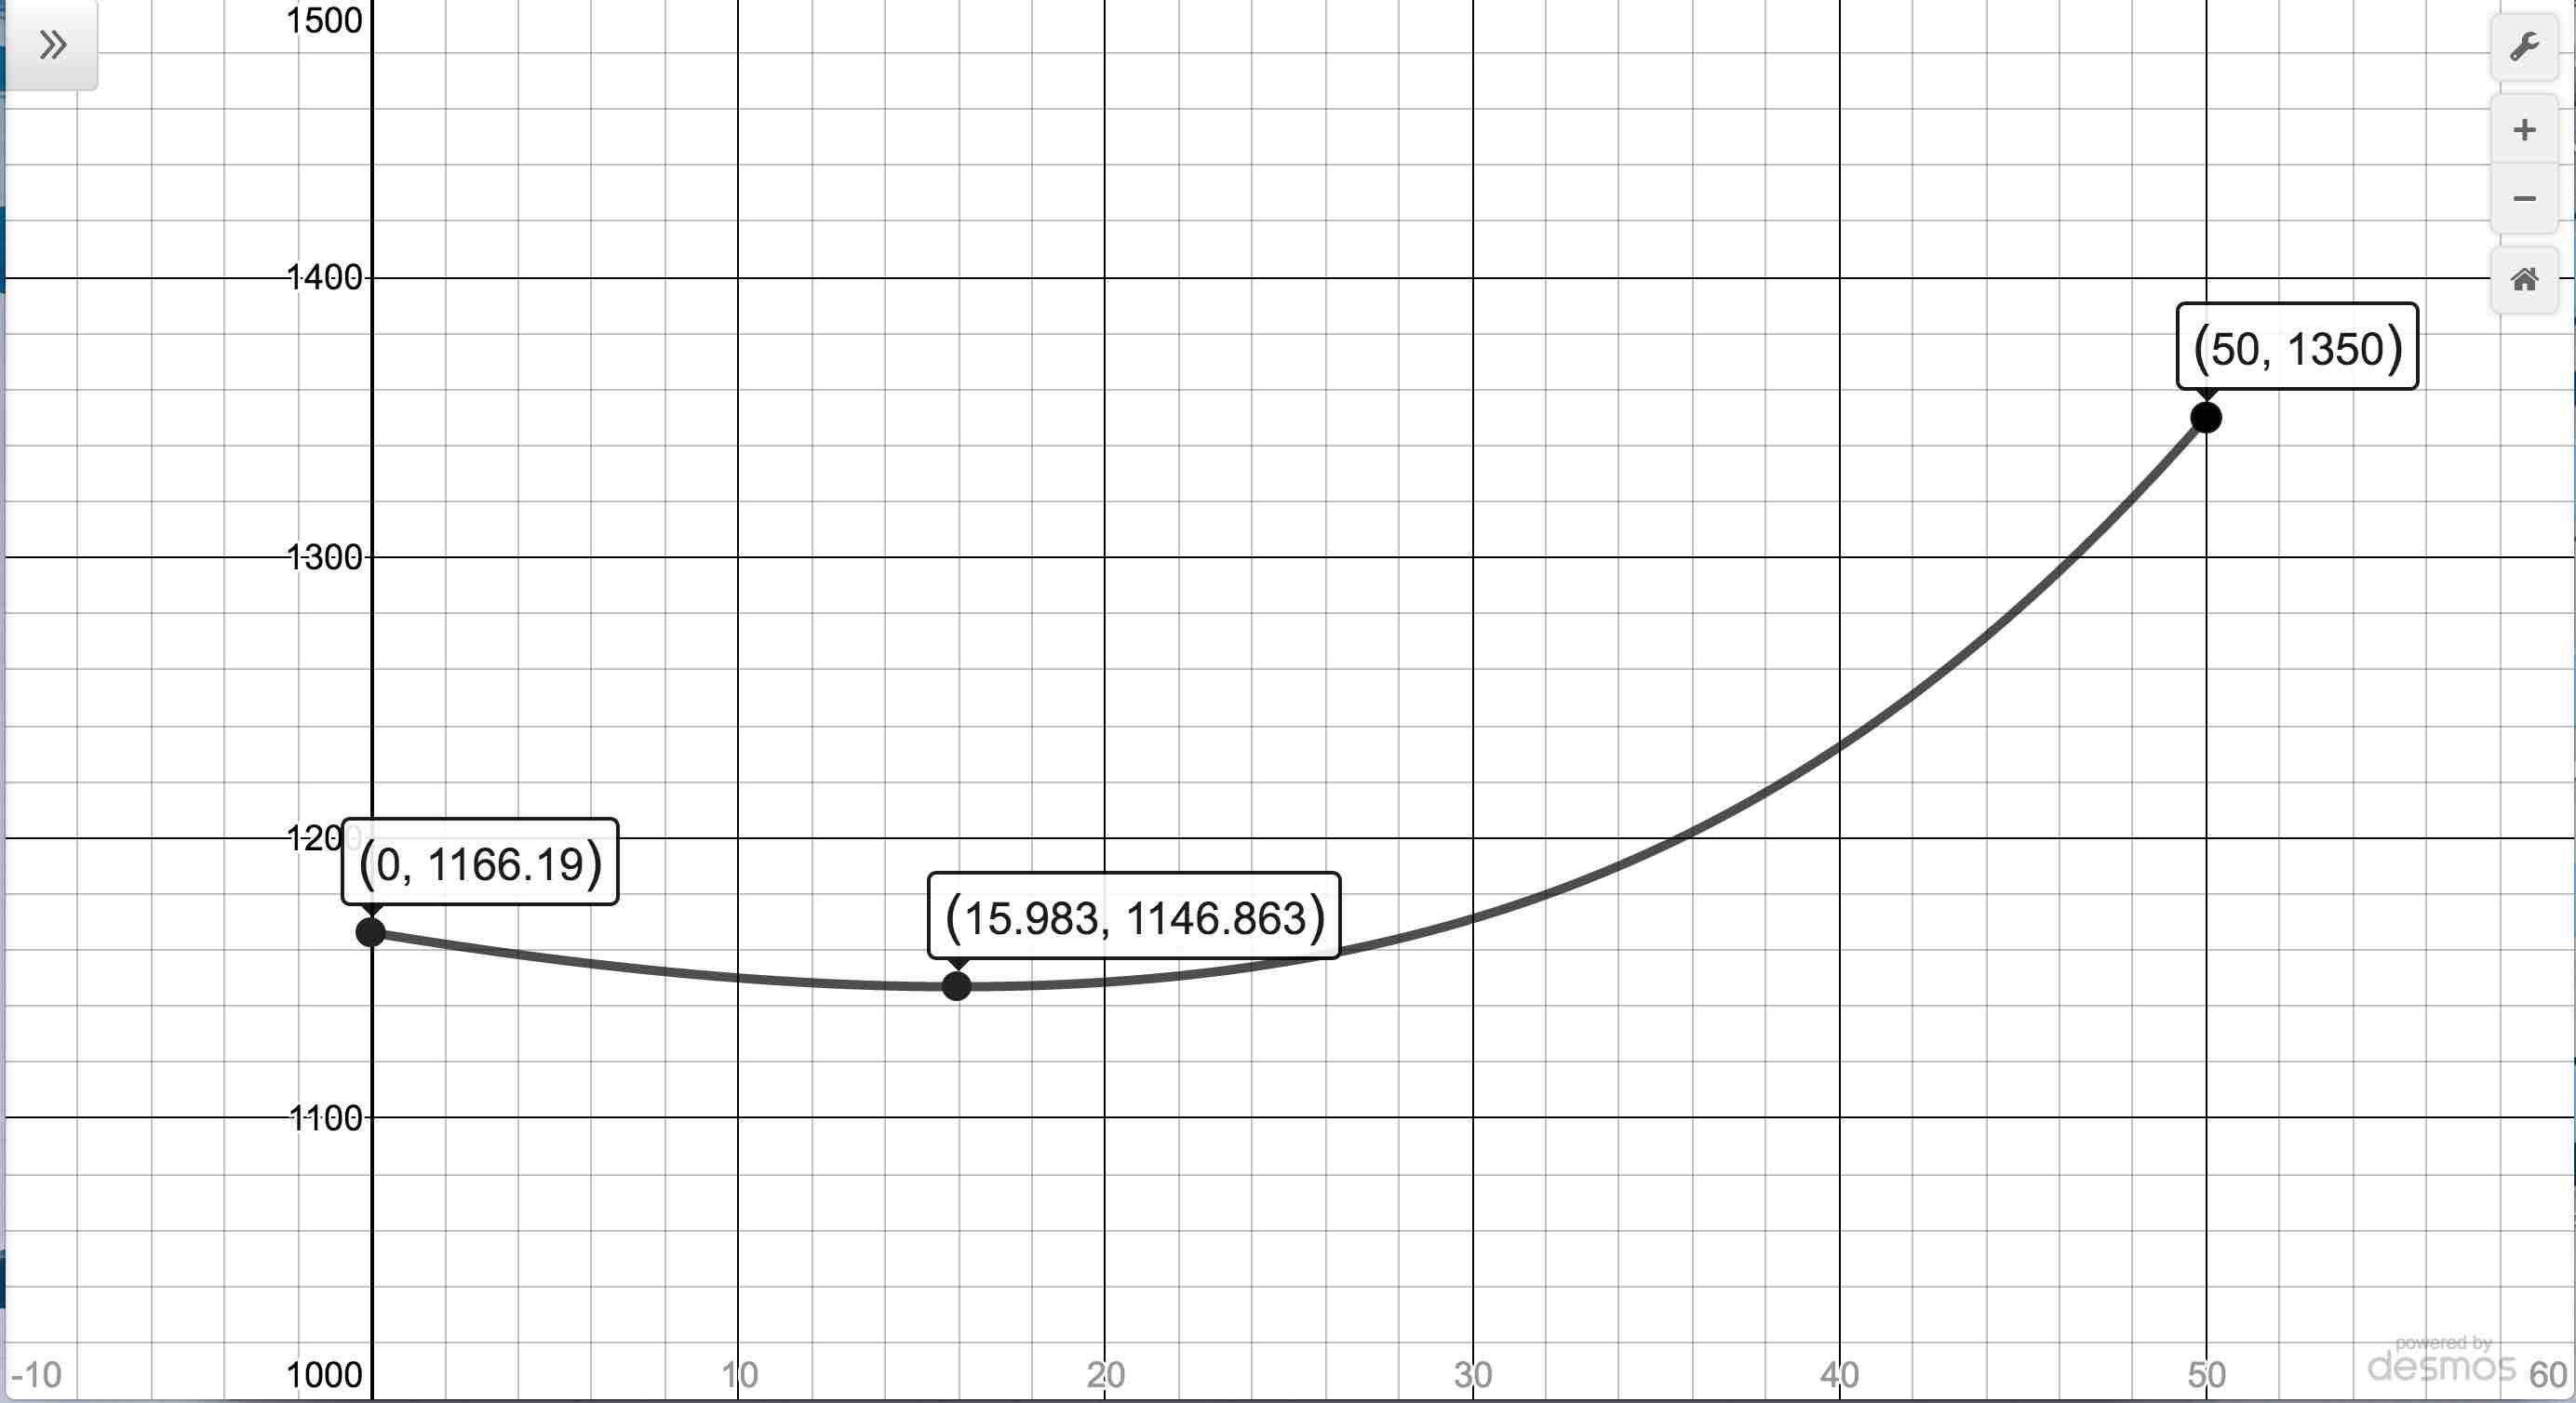
\includegraphics[width=4in]{./RootRadicalFunctionsGraphics/CostCableEx.jpg}}


 \qed

\end{enumerate}

\end{ex}

\newpage

\subsection{Exercises}

In Exercises \ref{radicalgraphexfirst} - \ref{radicalgraphexlast},  given the pair of functions $f$ and $F$, sketch the graph of $y=F(x)$ by starting with the graph of $y = f(x)$ and using Theorem \ref{linearrootgraphs}.   Track at least two points and state the domain and range using interval notation.

\begin{multicols}{2}
\begin{enumerate}

\item $f(x) = \sqrt{x}$, $F(x) = \sqrt{x+3}-2$ \label{radicalgraphexfirst}
\item $f(x) = \sqrt{x}$, $F(x) = \sqrt{4-x}-1$ 

\setcounter{HW}{\value{enumi}}
\end{enumerate}
\end{multicols}

\begin{multicols}{2}
\begin{enumerate}
\setcounter{enumi}{\value{HW}}
\item $f(x) = \sqrt[3]{x}$, $F(x) = \sqrt[3]{x-1}-2$ 
\item $f(x) = \sqrt[3]{x}$, $F(x) = -\sqrt[3]{8x + 8} + 4$ 

\setcounter{HW}{\value{enumi}}
\end{enumerate}
\end{multicols}

\begin{multicols}{2}
\begin{enumerate}
\setcounter{enumi}{\value{HW}}

\item $f(x) = \sqrt[4]{x}$, $F(x) = \sqrt[4]{x-1}-2$
\item $f(x) = \sqrt[4]{x}$, $F(x) = -3\sqrt[4]{x - 7} +1$

\setcounter{HW}{\value{enumi}}
\end{enumerate}
\end{multicols}

\begin{multicols}{2}
\begin{enumerate}
\setcounter{enumi}{\value{HW}}

\item $f(x) = \sqrt[5]{x}$, $F(x) = \sqrt[5]{x + 2} + 3$
\item $f(x) = \sqrt[8]{x}$, $F(x) = \sqrt[8]{-x} - 2$ \label{radicalgraphexlast}
\setcounter{HW}{\value{enumi}}
\end{enumerate}
\end{multicols}

In Exercises \ref{findformulaforsqrtgraphfirst} - \ref{findformulaforsqrtgraphlast}, find a formula for each function below in the form $F(x) = a\sqrt{bx-h}+k$.

\smallskip

\textbf{NOTE:}  There may be more than one solution!

\begin{multicols}{2}

\begin{enumerate}
\setcounter{enumi}{\value{HW}}

\item $~$ \label{findformulaforsqrtgraphfirst}  $y=F(x)$ %$F(x) = -\sqrt{x+4}+2$

\begin{mfpic}[15]{-5}{5}{-1}{5}
\axes
\tlabel[cc](5,-0.5){\scriptsize $x$}
\tlabel[cc](0.5,5){\scriptsize $y$}
\tlabel[cc](-4, 2.5){\scriptsize $(-4,2)$}
%\tlabel[cc](-0.5,-1){\scriptsize $\left(0, \frac{1}{2} \right)$}
\xmarks{-4,-3,-2,-1,1,2,3,4}
\ymarks{1,2,3,4}
\tlpointsep{4pt}
\scriptsize
\axislabels {x}{ {$-4 \hspace{7pt}$} -4, {$-3 \hspace{7pt}$} -3, {$-2 \hspace{7pt}$} -2, {$-1 \hspace{7pt}$} -1,  {$3$} 3, {$4$} 4}
\axislabels {y}{{$1$} 1, {$2$} 2, {$3$} 3, {$4$} 4}
\penwd{1.25pt}
\arrow  \function{-4,5,0.1}{2-sqrt(x+4)}
\point[4pt]{(-4,2), (0,0)}
\tcaption{ \scriptsize $x$,$y$-intercept $(0,0)$}
\normalsize
\end{mfpic} 



\item $~$ \label{findformulaforsqrtgraphlast} $y = F(x)$ %$F(x) =2\sqrt{-x+1}$

\begin{mfpic}[15]{-5}{5}{-1}{5}
\axes
\tlabel[cc](5,-0.5){\scriptsize $x$}
\tlabel[cc](0.5,5){\scriptsize $y$}
%\tlabel[cc](-1.5, 0.5){\scriptsize $(-1,0)$}
%\tlabel[cc](-0.5,-1){\scriptsize $\left(0, \frac{1}{2} \right)$}
\xmarks{-4,-3,-2,-1,1,2,3,4}
\ymarks{1,2,3,4}
\tlpointsep{4pt}
\scriptsize
\axislabels {x}{ {$-4 \hspace{7pt}$} -4, {$-3 \hspace{7pt}$} -3, {$-2 \hspace{7pt}$} -2, {$-1 \hspace{7pt}$} -1, {$1$} 1, {$2$} 2, {$3$} 3, {$4$} 4}
\axislabels {y}{{$1$} 1, {$2$} 2, {$3$} 3, {$4$} 4}
\penwd{1.25pt}
\arrow \reverse \function{-5,1,0.1}{2*sqrt(1-x)}
\point[4pt]{(1,0), (0,2)}
\tcaption{ \scriptsize $x$-intercept $(1,0)$, $y$-intercept $(0,2)$}
\normalsize
\end{mfpic} 


\setcounter{HW}{\value{enumi}}

\end{enumerate}

\end{multicols}

In Exercises \ref{findformulaforcubedrootgraphfirst} - \ref{findformulaforcubedrootgraphlast}, find a formula for each function below in the form $F(x) = a\sqrt[3]{bx-h}+k$.

\smallskip

\textbf{NOTE:}  There may be more than one solution!

\begin{multicols}{2}
\begin{enumerate}
\setcounter{enumi}{\value{HW}}

\item $~$ \label{findformulaforcubedrootgraphfirst}  $y=F(x)$ %$F(x) = -\sqrt[3]{2x+1}$

\begin{mfpic}[15]{-5}{5}{-5}{5}
\axes
\tlabel[cc](5,-0.5){\scriptsize $x$}
\tlabel[cc](0.5,5){\scriptsize $y$}
\tlabel[cc](-1, 1.75){\scriptsize $(-1,1)$}
%\tlabel[cc](-0.5,-1){\scriptsize $\left(0, \frac{1}{2} \right)$}
\xmarks{-4,-3,-2,-1,1,2,3,4}
\ymarks{-4,-3,-2, -1, 1,2,3,4}
\tlpointsep{4pt}
\scriptsize
\axislabels {x}{ {$-4 \hspace{7pt}$} -4, {$-3 \hspace{7pt}$} -3, {$-2 \hspace{7pt}$} -2, {$-1 \hspace{7pt}$} -1,  {$3$} 3, {$4$} 4}
\axislabels {y}{{$-1$} -1, {$3$} 3, {$4$} 4, {$-2$} -2, {$-3$} -3, {$-4$} -4}
\penwd{1.25pt}
 \arrow \reverse \arrow \parafcn{-2.25,2,0.1}{((0-0.5*(t**3))-0.5,t)}
\point[4pt]{(-0.5,0), (0,-1), (-1,1)}
\tcaption{ \scriptsize $x$-intercept $\left(-\frac{1}{2}, 0\right)$,$y$-intercept $(0,-1)$}
\normalsize
\end{mfpic} 



\item $~$ \label{findformulaforcubedrootgraphlast} $y = F(x)$ %$F(x) =2\sqrt[3]{x-1}-2$

\begin{mfpic}[15]{-5}{5}{-5}{5}
\axes
\tlabel[cc](5,-0.5){\scriptsize $x$}
\tlabel[cc](0.5,5){\scriptsize $y$}
\tlabel[cc](2, -2){\scriptsize $(1,-2)$}
\xmarks{-4,-3,-2,-1,1,2,3,4}
\ymarks{-4,-3,-2, -1, 1,2,3,4}
\tlpointsep{4pt}
\scriptsize
\axislabels {x}{ {$-4 \hspace{7pt}$} -4, {$-3 \hspace{7pt}$} -3, {$-2 \hspace{7pt}$} -2, {$-1 \hspace{7pt}$} -1, {$1$} 1, {$2$} 2, {$3$} 3, {$4$} 4}
\axislabels {y}{{$-1$} -1,{$1$} 1, {$2$} 2, {$3$} 3, {$4$} 4, {$-2$} -2, {$-3$} -3, {$-4$} -4}
\penwd{1.25pt}
 \arrow \reverse \arrow \parafcn{-5,1,0.1}{(  (0.125*((t+2)**3))+1 ,t)}
\point[4pt]{(2,0), (0,-4), (1,-2)}
\tcaption{ \scriptsize $x$-intercept $(2,0)$, $y$-intercept $(0,-4)$}
\normalsize
\end{mfpic} 


\setcounter{HW}{\value{enumi}}
\end{enumerate}
\end{multicols}

\begin{enumerate}
\setcounter{enumi}{\value{HW}}



\item  \label{rootstosolvepolyineq} Use the fact that the $n$th root functions are increasing to solve the following polynomial inequalities:

\begin{multicols}{3}

\begin{enumerate}

\item  $x^3 \leq 64$  \vphantom{$\dfrac{(2x+1)^3}{4} < 2$ }  % $(-\infty, 4]$

\item  $2 - t^5 <  34$  \vphantom{$\dfrac{(2x+1)^3}{4} < 2$ }  % $(-2, \infty)$

\item $\dfrac{(2z+1)^3}{4} \geq 2$ % $\left[ -\frac{1}{2}, \infty \right)$

\setcounter{HWindent}{\value{enumii}}

\end{enumerate}
\end{multicols}

For the following inequalities, remember $\sqrt[n]{x^{n}} = |x|$ if $n$ is even:

\begin{multicols}{3}

\begin{enumerate}
\setcounter{enumii}{\value{HWindent}}

\item  $x^4 \leq 16$  \vphantom{$\dfrac{(2x+1)^3}{4} < 2$ }  % $[-2,2]$

\item  $6-t^6 < -58$  \vphantom{$\dfrac{(2x+1)^3}{4} < 2$ }  % $(-\infty, -2) \cup (2, \infty)$

\item $\dfrac{(2z+1)^4}{3} \geq 27$ % $(-\infty, -2] \cup [1, \infty)$

\end{enumerate}

\end{multicols}

\setcounter{HW}{\value{enumi}}
\end{enumerate}


For each function in Exercises \ref{algfcngraphexfirst} - \ref{algfcngraphexlast} below 

\begin{itemize}

\item Analytically:

\begin{multicols}{3}

\begin{itemize}

\item find the domain.

\item find the axis intercepts.

\item analyze the end behavior.

\end{itemize}

\end{multicols}

\item Graph the function with help from a graphing utility and determine:

\begin{multicols}{2}

\begin{itemize}

\item  the range.

\item the local extrema, if they exist.

\end{itemize}

\end{multicols}

\begin{multicols}{2}

\begin{itemize}

\item intervals of increase/decrease.

\item any `unusual steepness' or `local' verticality.

\end{itemize}

\end{multicols}

\begin{multicols}{2}

\begin{itemize}

\item  vertical asymptotes.

\item  horizontal / slant asymptotes.

\end{itemize}

\end{multicols}

\item Construct a sign diagram for each function using the intercepts and graph.

\item  Comment on any observed symmetry.


\end{itemize}

\begin{multicols}{2}
\begin{enumerate}
\setcounter{enumi}{\value{HW}}
\item $f(x) = \sqrt{1 - x^{2}}$ \label{algfcngraphexfirst}
\item $f(x) = \sqrt{x^2-1}$

\setcounter{HW}{\value{enumi}}
\end{enumerate}
\end{multicols}

\begin{multicols}{2}
\begin{enumerate}
\setcounter{enumi}{\value{HW}}

\item $g(t) = t \sqrt{1-t^2}$
\item $g(t) = t \sqrt{t^2-1}$

\setcounter{HW}{\value{enumi}}
\end{enumerate}
\end{multicols}

\begin{multicols}{2}
\begin{enumerate}
\setcounter{enumi}{\value{HW}}

\item $f(x) = \sqrt[4]{\dfrac{16x}{x^{2} - 9}}$
\item $f(x) = \dfrac{5x}{\sqrt[3]{x^{3} + 8}}$
\setcounter{HW}{\value{enumi}}
\end{enumerate}
\end{multicols}


\begin{multicols}{2}
\begin{enumerate}
\setcounter{enumi}{\value{HW}}

\item $g(t) = \sqrt{t(t + 5)(t - 4)}$
\item $g(t) = \sqrt[3]{t^{3} + 3t^{2} - 6t - 8}$ \label{algfcngraphexlast}

\setcounter{HW}{\value{enumi}}
\end{enumerate}
\end{multicols}



\begin{enumerate}
\setcounter{enumi}{\value{HW}}

\item  Rework Example \ref{SasquatchCable} so that the outpost is 10 miles from Route 117 and the nearest junction box is 30 miles down the road for the post.


\item  The volume $V$ of a right cylindrical cone depends on the radius of its base $r$ and its height $h$ and is given by the formula $V = \frac{1}{3} \pi r^2 h$.  The surface area $S$ of a right cylindrical cone also depends on $r$ and $h$ according to the formula $S = \pi r \sqrt{r^2+h^2}$.  In the following problems, suppose a cone is to have a volume of 100 cubic centimeters. 

\begin{enumerate}

\item  \label{heightintermsofr} Use the formula for volume to find the height as a function of $r$, $h(r)$.
\item  Use the formula for surface area along with  your answer to \ref{heightintermsofr} to find the surface area as a function of $r$, $S(r)$.
\item  Use your calculator to find the values of $r$ and $h$ which minimize the surface area.  What is the minimum surface area?  Round your answers to two decimal places.

\end{enumerate}


\item \label{pendulumproblem} The period of a pendulum in seconds is given by \[T = 2\pi \sqrt{\dfrac{L}{g}}\](for small displacements) where $L$ is the length of the pendulum in meters and $g = 9.8$ meters per second per second is the acceleration due to gravity.  My Seth-Thomas antique schoolhouse clock needs $T = \frac{1}{2}$ second and I can adjust the length of the pendulum via a small dial on the bottom of the bob.  At what length should I set the pendulum?


\item According to Einstein's Theory of Special Relativity, the observed mass  of an object is a function of how fast the object is traveling.  Specifically, if  $m_{r}$ is the mass of the object at rest, $v$ is the speed of the object and $c$ is the speed of light, then the observed mass of the object $m(v)$ is given by:
\[m(v) = \dfrac{m_{r}}{\sqrt{1 - \dfrac{v^{2}}{c^{2}}}}\] 

\begin{enumerate}

\item Find the applied domain of the function.

\item Compute $m(.1c), \, m(.5c), \, m(.9c)$ and $m(.999c)$.

\item Find $\ds{\lim_{v \rightarrow c^{-}} m(v)}$.

\item How slowly must the object be traveling so that the observed mass is no greater than 100 times its mass at rest?

\end{enumerate}


\item Find the inverse of $k(x) = \dfrac{2x}{\sqrt{x^{2} - 1}}$.




\end{enumerate}

\newpage

\subsection{Answers}

\begin{multicols}{2}
\begin{enumerate}


\item $F(x) = \sqrt{x+3}-2$ \\ 

\begin{mfpic}[15]{-5}{5}{-3}{5}
\axes
\tlabel[cc](5,-0.5){\scriptsize $x$}
\tlabel[cc](0.5,5){\scriptsize $y$}
\point[4pt]{(-3,-2), (-2,-1), (1,0)}
\ymarks{-2,-1,1,2,3,4}
\xmarks{-4,-3,-2,-1,1,2,3,4}
\tiny
\tlpointsep{4pt}
\axislabels {y}{{$-2$} -2, {$-1$} -1, {$1$} 1,{$2$} 2, {$3$} 3,{$4$} 4 }
\axislabels {x}{{$-4 \hspace{7pt}$} -4, {$-3 \hspace{7pt}$} -3, {$-2 \hspace{7pt}$} -2, {$-1 \hspace{7pt}$} -1, {$1$} 1,  {$2$} 2, {$3$} 3,  {$4$} 4}
\normalsize
\penwd{1.25pt}
 \arrow \parafcn{-2,0.8,0.1}{(((t+2)**2)-3,t)}
 \tcaption{Domain:  $[-3, \infty)$, Range: $[-2, \infty)$}
\end{mfpic}

\vfill

\columnbreak

\item $F(x) = \sqrt{4-x}-1 = \sqrt{-x+4} - 1$ \\

\begin{mfpic}[15]{-5}{5}{-3}{5}
\axes
\tlabel[cc](5,-0.5){\scriptsize $x$}
\tlabel[cc](0.5,5){\scriptsize $y$}
\point[4pt]{(4,-1), (3,0), (0,1)}
\ymarks{-2,-1,1,2,3,4}
\xmarks{-4,-3,-2,-1,1,2,3,4}
\tiny
\tlpointsep{4pt}
\axislabels {y}{{$-2$} -2, {$-1$} -1, {$1$} 1,{$2$} 2, {$3$} 3,{$4$} 4 }
\axislabels {x}{{$-4 \hspace{7pt}$} -4, {$-3 \hspace{7pt}$} -3, {$-2 \hspace{7pt}$} -2, {$-1 \hspace{7pt}$} -1, {$1$} 1,  {$2$} 2, {$3$} 3,  {$4$} 4}
\normalsize
\penwd{1.25pt}
 \arrow \parafcn{-1,2,0.1}{(4-((t+1)**2),t)}
  \tcaption{Domain:  $(-\infty, 4]$, Range: $[-1, \infty)$}
\end{mfpic}


\setcounter{HW}{\value{enumi}}
\end{enumerate}
\end{multicols}


\begin{multicols}{2}
\begin{enumerate}
\setcounter{enumi}{\value{HW}}


\item $F(x) = \sqrt[3]{x-1}-2$ \\ 

\begin{mfpic}[8][13]{-10}{12}{-5}{1}
\axes
\tlabel[cc](12,-0.5){\scriptsize $x$}
\tlabel[cc](0.75,1){\scriptsize $y$}
\point[4pt]{(-7, -4), (0,-3), (1,-2), (2,-1), (9,0)}
\ymarks{-4,-3,-2,-1}
\xmarks{-9 step 1 until 11}
\tiny
\tlpointsep{4pt}
\axislabels {y}{{$-4$} -4, {$-3$} -3, {$-2$} -2, {$-1$} -1}
\axislabels {x}{{$-9 \hspace{6pt}$} -9, {$-7 \hspace{6pt}$} -7,  {$-5 \hspace{6pt}$} -5,  {$-3 \hspace{6pt}$} -3,  {$-1 \hspace{6pt}$} -1, {$1$} 1,  {$3$} 3, {$5$} 5,  {$7$} 7,  {$9$} 9, {$11$} 11}
\normalsize
\penwd{1.25pt}
\arrow \reverse \arrow \parafcn{-4.2,0.2,0.1}{(((t + 2)**3) + 1,t)}
 \tcaption{Domain:  $(-\infty, \infty)$, Range: $(-\infty, \infty)$}
\end{mfpic}

\vfill

\columnbreak

\item $F(x) = -\sqrt[3]{8x + 8} + 4$\\

\begin{mfpic}[10][9]{-7}{9}{-1}{8}
\axes
\tlabel[cc](9,-0.5){\scriptsize $x$}
\tlabel[cc](0.5,8){\scriptsize $y$}
\xmarks{-6 step 1 until 8}
\ymarks{1 step 1 until 7}
\tlpointsep{4pt}
\tiny
\axislabels {x}{ {$-5 \hspace{6pt}$} -5,  {$-3 \hspace{6pt}$} -3, {$-1 \hspace{6pt}$} -1, {$1$} 1,  {$3$} 3,  {$5$} 5,  {$7$} 7 }
\axislabels {y}{{$1$} 1, {$2$} 2, {$3$} 3, {$4$} 4, {$5$} 5, {$6$} 6, {$7$} 7}
\normalsize
\point[4pt]{(-2,6),(-1,4),(0,2),(7,0)}
\penwd{1.25pt}
\arrow \reverse \function{-7,-1,0.1}{2*((-x - 1)**(1/3)) + 4}
\arrow \function{-1,8.5,0.1}{-2*((x + 1)**(1/3)) + 4}
 \tcaption{Domain:  $(-\infty, \infty)$, Range: $(-\infty, \infty)$}
\end{mfpic}

\setcounter{HW}{\value{enumi}}
\end{enumerate}
\end{multicols}


\begin{multicols}{2}
\begin{enumerate}
\setcounter{enumi}{\value{HW}}


\item $F(x) = \sqrt[4]{x-1}-2$\\

\begin{mfpic}[8][25]{-1}{22}{-3}{1}
\axes
\tlabel[cc](22,-0.75){\scriptsize $x$}
\tlabel[cc](0.5,1){\scriptsize $y$}
\point[4pt]{(1,-2),(2,-1),(17,0)}
\ymarks{-2,-1}
\xmarks{1 step 1 until 21}
\tiny
\tlpointsep{4pt}
\axislabels {y}{{$-2$} -2, {$-1$} -1}
\axislabels {x}{{$1$} 1,  {$3$} 3, {$5$} 5, {$7$} 7,  {$9$} 9,  {$11$} 11,  {$13$} 13,  {$15$} 15,  {$17$} 17, {$19$} 19,  {$21$} 21}
\normalsize
\penwd{1.25pt}
\arrow \parafcn{-2,0.12,0.1}{(((t + 2)**4) + 1,t)}
 \tcaption{Domain:  $[1, \infty)$, Range: $[-2, \infty)$}
\end{mfpic}

\vfill

\columnbreak

\item $F(x) = -3\sqrt[4]{x - 7} +1$\\

\begin{mfpic}[5][13]{-1}{25}{-6}{2}
\axes
\tlabel[cc](25,-0.5){\scriptsize $x$}
\tlabel[cc](0.5,2){\scriptsize $y$}
\xmarks{1 step 1 until 23}
\ymarks{-5 step 1 until 1}
\tlpointsep{4pt}
\tiny
\axislabels {x}{ {$6$} 6, {$8$} 8, {$23$} 23}
\axislabels {y}{{$1$} 1, {$-1$} -1, {$-2$} -2, {$-3$} -3, {$-4$} -4, {$-5$} -5}
\normalsize
\point[4pt]{(7,1),(8,-2),(23,-5)}
\penwd{1.25pt}
\arrow \function{7,25,0.1}{1-3*((x - 7)**(0.25)) }
 \tcaption{Domain:  $[7, \infty)$, Range: $(-\infty, 1]$}
\end{mfpic}

\setcounter{HW}{\value{enumi}}
\end{enumerate}
\end{multicols}

\newpage

\begin{multicols}{2}
\begin{enumerate}
\setcounter{enumi}{\value{HW}}

\item $F(x) = \sqrt[5]{x + 2} + 3$\\

\begin{mfpic}[2][10]{-37}{33}{-1}{6}
\axes
\tlabel[cc](33,-0.5){\scriptsize $x$}
\tlabel[cc](2,6){\scriptsize $y$}
\xmarks{-34,-2,30}
\ymarks{1 step 1 until 5}
\tlpointsep{4pt}
\tiny
\axislabels {x}{{$-34 \hspace{5pt}$} -34, {$-2 \hspace{5pt}$} -2, {$30$} 30}
\axislabels {y}{{$1$} 1, {$2$} 2, {$3$} 3, {$4$} 4, {$5$} 5}
\normalsize
\point[4pt]{(-34,1),(-3,2),(-2,3),(-1,4),(30,5)}
\penwd{1.25pt}
\arrow \function{-2,33,0.1}{((x + 2)**(0.20)) + 3}
\arrow \reverse \function{-37,-2,0.1}{(-((-x - 2)**(0.20))) + 3}
 \tcaption{Domain:  $(-\infty, \infty)$, Range: $(-\infty, \infty)$}
\end{mfpic}

\item $F(x) = \sqrt[8]{-x} - 2$\\

\begin{mfpic}[3][15]{-45}{5}{-3}{1}
\axes
\tlabel[cc](5,-0.5){\scriptsize $x$}
\tlabel[cc](1.5,1){\scriptsize $y$}
\xmarks{-40,-30,-20,-10}
\ymarks{-2,-1}
\tlpointsep{4pt}
\tiny
\axislabels {x}{ {$-20 \hspace{5pt}$} -20, {$-10 \hspace{5pt}$} -10}
\axislabels {y}{{$-2$} -2}
\normalsize
\point[4pt]{(0,-2),(-1,-1)}
\penwd{1.25pt}
\arrow \reverse \function{-45,0,0.1}{((-x)**0.125) - 2}
 \tcaption{Domain:  $(-\infty, 0]$, Range: $[-2, \infty)$}
\end{mfpic}

\setcounter{HW}{\value{enumi}}
\end{enumerate}
\end{multicols}

\begin{multicols}{2}

\begin{enumerate}
\setcounter{enumi}{\value{HW}}

\item One solution is: $F(x) = -\sqrt{x+4}+2$


\item One solution is: $F(x) =2\sqrt{-x+1}$

\setcounter{HW}{\value{enumi}}

\end{enumerate}

\end{multicols}

\begin{multicols}{2}
\begin{enumerate}
\setcounter{enumi}{\value{HW}}

\item One solution is:  $F(x) = -\sqrt[3]{2x+1}$

\item One solution is:  $F(x) =2\sqrt[3]{x-1}-2$

\setcounter{HW}{\value{enumi}}
\end{enumerate}
\end{multicols}

\begin{enumerate}
\setcounter{enumi}{\value{HW}}

\item 

\begin{multicols}{3}

\begin{enumerate}

\item   $(-\infty, 4]$  \vphantom{$\left[ \frac{1}{2}, \infty \right)$}

\item   $(-2, \infty)$ \vphantom{$\left[ \frac{1}{2}, \infty \right)$}

\item $\left[ \frac{1}{2}, \infty \right)$

\setcounter{HWindent}{\value{enumii}}

\end{enumerate}
\end{multicols}

\begin{multicols}{3}

\begin{enumerate}
\setcounter{enumii}{\value{HWindent}}

\item   $[-2,2]$

\item   $(-\infty, -2) \cup (2, \infty)$

\item   $(-\infty, -2] \cup [1, \infty)$

\end{enumerate}

\end{multicols}

\setcounter{HW}{\value{enumi}}
\end{enumerate}



\begin{enumerate}
\setcounter{enumi}{\value{HW}}
\item \begin{multicols}{2}
$f(x) = \sqrt{1 - x^2}$\\
Domain: $[-1, 1]$\\
Intercepts: $(-1,0)$, $(1,0)$ \\
Range: $[0,1]$\\
Local maximum: $(0,1)$\\
Increasing: $[-1,0]$, Decreasing: $[0,1]$\\
Unusual steepness\footnote{You may need to zoom in to see this.} at $x = -1$ and $x = 1$\\
Sign Diagram: \\

\smallskip

\begin{mfpic}[20][10]{0}{4}{-1.5}{1.5}
\polyline{(0,0), (4,0)}
\xmarks{0,4}
\tlabel[cc](0,-1){$-1 \hspace{7pt}$}
\tlabel[cc](2,1){$(+)$}
\tlabel[cc](0,1){$0$}
\tlabel[cc](4,1){$0$}
\tlabel[cc](4,-1){$1$}
\end{mfpic}


\columnbreak

Graph: \\

\begin{mfpic}[50]{-1.5}{1.5}{-0.15}{1.5}
\axes
\tlabel[cc](1.5,-0.15){\scriptsize $x$}
\tlabel[cc](0.25,1.5){\scriptsize $y$}
\tlabel[cc](0.25,1.15){\scriptsize $(0,1)$}
\xmarks{-1,1}
\ymarks{1}
\tlpointsep{4pt}
\scriptsize
\axislabels {x}{{$-1 \hspace{6pt}$} -1, {$1$} 1}
%\axislabels {y}{{$1$} 1}
\normalsize
\point[4pt]{(0,1), (-1,0), (1,0)}
\penwd{1.25pt}
\parafcn{0,3.14159,0.1}{(cos(t),sin(t))}
\end{mfpic}



Note:  $f$ is even.

\end{multicols}

\pagebreak

\item \begin{multicols}{2}
$f(x) = \sqrt{x^2-1}$\\
Domain: $(-\infty, -1] \cup [1,\infty)$\\
Intercepts: $(-1,0)$, $(1,0)$\\
$\ds{\lim_{x \rightarrow -\infty} f(x) = \infty}$\\
\footnote{Using Calculus, one can show $y = -x$ and $y = -x$ are slant asymptotes to the graph.}$\ds{\lim_{x \rightarrow \infty} f(x) = \infty}$\\
Range:   $[0, \infty)$ \\
Increasing: $[1, \infty)$, Decreasing: $(-\infty, -1]$ \\
Unusual steepness\footnote{You may need to zoom in to see this.}at $x = -1$ and $x = 1$\\
Sign Diagram: \\

\smallskip
\begin{mfpic}[20][10]{0}{4}{-1.5}{1.5}
\arrow \polyline{(2,0), (0,0)}
\arrow \polyline{(3,0), (5,0)}
\xmarks{2,3}
\tlabel[cc](2,-1){$-1 \hspace{7pt}$}
\tlabel[cc](1,1){$(+)$}
\tlabel[cc](4,1){$(+)$}
\tlabel[cc](2,1){$0$}
\tlabel[cc](3,1){$0$}
\tlabel[cc](3,-1){$1$}
\end{mfpic}

\columnbreak

Graph: \\

\begin{mfpic}[20]{-4}{4}{-1}{4}
\axes
\tlabel[cc](4,-0.25){\scriptsize $x$}
\tlabel[cc](0.25,4){\scriptsize $y$}
\xmarks{-3,-2,-1,1,2,3}
\ymarks{1,2,3}
\tlpointsep{4pt}
\scriptsize
\axislabels {x}{{$-3 \hspace{6pt}$} -3,{$-2 \hspace{6pt}$} -2,{$-1 \hspace{6pt}$} -1, {$1$} 1, {$2$} 2, {$3$} 3}
\axislabels {y}{{$1$} 1, {$2$} 2, {$3$} 3}
\normalsize
\point[4pt]{(-1,0), (1,0)}
\dashed \polyline{(0,0), (4,4)}
\dashed \polyline{(0,0), (-4,4)}
\penwd{1.25pt}
\arrow \parafcn{0,2,0.1}{(cosh(t),sinh(t))}
\arrow \parafcn{0,2,0.1}{(-cosh(t),sinh(t))}
\end{mfpic}

Note:  $f$ is even.

\end{multicols}



\item \begin{multicols}{2}
$g(t) = t\sqrt{1-t^2}$\\
Domain: $[-1,1]$\\
Intercepts: $(-1,0)$, $(0,0)$, $(1,0)$\\
Range:  $\approx [-0.5, 0.5]$\\
Local minimum $\approx (-0.707, -0.5)$ \\
Local maximum:  $\approx (0.707, 0.5)$\\
Increasing: $\approx [-0.707, 0.707]$ \\
Decreasing:  $\approx [-1, -0.707]$, $[0.707, 1]$\\
Unusual steepness at $t = -1$ and $t = 1$\\
Sign Diagram:\\

\begin{mfpic}[20][10]{0}{4}{-1.5}{1.5}
\polyline{(0,0), (5,0)}
\xmarks{0,2.5,5}
\tlabel[cc](0,-1){$-1 \hspace{7pt}$}
\tlabel[cc](0,1){$0$}
\tlabel[cc](1.25,1){$(-)$}
\tlabel[cc](2.5,-1){$0$}
\tlabel[cc](3.75,1){$(+)$}
\tlabel[cc](2.5,1){$0$}
\tlabel[cc](5,-1){$1$}
\tlabel[cc](5,1){$0$}
\end{mfpic}

\columnbreak

Graph:\\

\begin{mfpic}[50][40]{-1.5}{1.5}{-1}{1.5}
\axes
\tlabel[cc](1.5,-0.15){\scriptsize $t$}
\tlabel[cc](0.25,1.5){\scriptsize $y$}
\tlabel[cc](-1,0.15){\scriptsize $-1\hspace{7pt}$}
\tlabel[cc](0.7,0.7){\scriptsize $\approx (0.707, 0.5)$}
\tlabel[cc](-0.7,-0.7){\scriptsize $\approx (-0.707, -0.5)$}
\xmarks{-1,1}
\ymarks{-1,1}
\tlpointsep{4pt}
\scriptsize
\axislabels {x}{ {$1$} 1}
\axislabels {y}{{$1$} 1,{$-1$} -1}
\normalsize
\point[4pt]{(-1,0), (1,0),(0,0),  (-0.707, -0.5),  (0.707, 0.5)}
\penwd{1.25pt}
\parafcn{0,3.14159,0.1}{(cos(t),cos(t)*sin(t))}
\end{mfpic}

Note:  $g$ is odd.

\end{multicols}

\item \begin{multicols}{2}
$g(t) = t\sqrt{t^2-1}$\\
Domain: $(-\infty, -1] \cup [1,\infty)$\\
Intercepts: $(-1,0)$, $(1,0)$\\
$\ds{\lim_{t \rightarrow -\infty} g(t) = -\infty}$ \\
$\ds{\lim_{t \rightarrow \infty} g(t) = \infty}$ \\
Range: $(-\infty, \infty)$\\
Increasing: $(-\infty, -1]$, $[1, \infty)$\\
Unusual steepness at $t = -1$ and $t = 1$\\
Sign Diagram:\\

\smallskip
\begin{mfpic}[20][10]{0}{4}{-1.5}{1.5}
\arrow \polyline{(2,0), (0,0)}
\arrow \polyline{(3,0), (5,0)}
\xmarks{2,3}
\tlabel[cc](2,-1){$-1 \hspace{7pt}$}
\tlabel[cc](1,1){$(-)$}
\tlabel[cc](4,1){$(+)$}
\tlabel[cc](2,1){$0$}
\tlabel[cc](3,1){$0$}
\tlabel[cc](3,-1){$1$}
\end{mfpic}

\columnbreak

Graph:\\

\begin{mfpic}[20][15]{-4}{4}{-4}{4}
\axes
\tlabel[cc](4,-0.25){\scriptsize $t$}
\tlabel[cc](0.25,4){\scriptsize $y$}
\xmarks{-3,-2,-1,1,2,3}
\ymarks{-3,-2,-1,1,2,3}
\tlpointsep{4pt}
\scriptsize
\axislabels {x}{{$-3 \hspace{6pt}$} -3,{$-2 \hspace{6pt}$} -2,{$-1 \hspace{6pt}$} -1, {$1$} 1, {$2$} 2, {$3$} 3}
\axislabels {y}{{$-3$} -3,{$-2$} -2,{$-1$} -1,{$1$} 1, {$2$} 2, {$3$} 3}
\normalsize
\point[4pt]{(-1,0), (1,0)}
\penwd{1.25pt}
\arrow \reverse \function{-1.9,-1,0.1}{x*sqrt((x**2)-1)}
\arrow \function{1,1.9,0.1}{x*sqrt((x**2)-1)}
\end{mfpic}


Note:  $g$ is odd.

\end{multicols}



\item \begin{multicols}{2} 
$f(x) = \sqrt[4]{\dfrac{16x}{x^2 - 9}}$\\
Domain: $(-3, 0] \cup (3, \infty)$\\
Intercept: $(0,0)$\\
Range:  $[0, \infty)$\\
Decreasing: $(-3, 0]$, $(3, \infty)$\\
Unusual steepness at $x = 0$ \\
Vertical asymptotes: $x = -3$ and $x = 3$\\
Horizontal asymptote: $y = 0$\\
Sign Diagram: \\

\smallskip

\begin{mfpic}[15]{-3}{6}{-1}{1}
\polyline{(-3,0),(0,0)}
\arrow  \polyline{(3,0),(6,0)}
\xmarks{-3,0,3}
\tlabel[cc](-1.5,0.75){$(+)$}
\tlabel[cc](-3,-0.75){$-3 \hspace{7pt}$}
\tlabel[cc](-3,0.75){\textinterrobang}
\tlabel[cc](0,-0.75){$0$}
\tlabel[cc](0,0.75){$0$}
\tlabel[cc](3,0.75){\textinterrobang}
\tlabel[cc](3,-0.75){$3$}
\tlabel[cc](4.5,0.75){$(+)$}
\end{mfpic}

\columnbreak


Graph:\\
\begin{mfpic}[15]{-3.5}{9}{-1}{6}
\axes
\tlabel[cc](9,-0.5){\scriptsize $x$}
\tlabel[cc](0.5,6){\scriptsize $y$}
\xmarks{-3 step 1 until 8}
\ymarks{1,2,3,4,5}
\tlpointsep{4pt}
\scriptsize
\axislabels {x}{{$-3 \hspace{6pt}$} -3, {$-2 \hspace{6pt}$} -2, {$-1 \hspace{6pt}$} -1, {$1$} 1, {$2$} 2, {$3$} 3, {$4$} 4, {$5$} 5, {$6$} 6, {$7$} 7, {$8$} 8}
\axislabels {y}{{$1$} 1, {$2$} 2, {$3$} 3, {$4$} 4, {$5$} 5}
\normalsize
\point[4pt]{(0,0)}
\dashed \polyline{(-3,-1), (-3,6)}
\dashed \polyline{(3,-1), (3,6)}
\penwd{1.25pt}
\arrow \reverse \function{-2.93,0,0.1}{((16*x)/((x**2) - 9))**(0.25)}
\arrow \reverse \arrow \function{3.05,9,0.1}{((16*x)/((x**2) - 9))**(0.25)}
\end{mfpic}

\end{multicols}

\item \begin{multicols}{2} 
$f(x) = \dfrac{5x}{\sqrt[3]{x^{3} + 8}}$\\
Domain: $(-\infty, -2) \cup (-2, \infty)$\\
Intercept:  $(0,0)$\\
Range:  $(-\infty, 5) \cup (5, \infty)$\\
Increasing: $(-\infty, -2)$, $(-2, \infty)$\\
Vertical asymptote $x = -2$\\
Horizontal asymptote $y = 5$\\
Sign Diagram:\\ 

\smallskip

\begin{mfpic}[20]{-4}{2}{-1}{1}
\arrow \reverse \arrow \polyline{(-4,0),(2,0)}
\xmarks{-2,0}
\tlabel[cc](-3, 0.5){$(+)$}
\tlabel[cc](-2,-0.5){$-2 \hspace{7pt}$}
\tlabel[cc](-2,0.5){\textinterrobang}
\tlabel[cc](-1,0.5){$(-)$}
\tlabel[cc](0,-0.5){$0$}
\tlabel[cc](0,0.5){$0$}
\tlabel[cc](1,0.5){$(+)$}
\end{mfpic}

\columnbreak

Graph: \\

\begin{mfpic}[10][8]{-5}{5}{-7}{9}
\axes
\tlabel[cc](5,-0.5){\scriptsize $x$}
\tlabel[cc](0.5,9){\scriptsize $y$}
\xmarks{-4 step 1 until 4}
\ymarks{-6 step 1 until 8}
\tlpointsep{4pt}
\tiny
\axislabels {x}{{$-4 \hspace{6pt}$} -4, {$-3 \hspace{6pt}$} -3, {$-2 \hspace{6pt}$} -2, {$-1 \hspace{6pt}$} -1, {$1$} 1, {$2$} 2, {$3$} 3, {$4$} 4}
\axislabels {y}{{$-6$} -6, {$-5$} -5, {$-4$} -4, {$-3$} -3,{$1$} 1, {$2$} 2, {$3$} 3, {$4$} 4, {$5$} 5, {$6$} 6, {$7$} 7, {$8$} 8}
\normalsize
\dashed \polyline{(-5,5), (5,5)}
\dashed \polyline{(-2,-7), (-2,9)}
\point[4pt]{(0,0)}
\penwd{1.25pt}
\arrow \reverse \arrow \function{-5,-2.2,0.1}{(-5*x)/((-(x**3) - 8)**(1/3))}
\arrow \reverse \arrow \function{-1.8,5,0.1}{(5*x)/(((x**3) + 8)**(1/3))}
\end{mfpic}

\end{multicols}



\item \begin{multicols}{2} 
$g(t) = \sqrt{t(t + 5)(t - 4)}$\\
Domain: $[-5, 0] \cup [4, \infty)$\\
Intercepts  $(-5,0)$, $(0,0)$, $(4,0)$\\
$\ds{\lim_{t \rightarrow \infty} g(t) = \infty}$\\
Range:  $[0, \infty)$\\
Local maximum $\approx (-2.937, 6.483)$\\
Increasing: $\approx [-5, -2.937]$, $[4, \infty)$\\
Decreasing: $\approx [-2.937,0]$\\
Unusual steepness at $t = -5, t = 0$ and $t = 4$\\
Sign Diagram:\\

\smallskip

\begin{mfpic}[10]{-5}{8}{-1}{1}
\polyline{(-5,0),(0,0)}
\arrow  \polyline{(4,0),(8,0)}
\xmarks{-5,0,4}
\tlabel[cc](-5,-1){$-5 \hspace{7pt}$}
\tlabel[cc](-5,1){$0$}
\tlabel[cc](-2.5,1){$(+)$}
\tlabel[cc](0,-1){$0$}
\tlabel[cc](0,1){$0$}
\tlabel[cc](4,-1){$4$}
\tlabel[cc](4,1){$0$}
\tlabel[cc](6,1){$(+)$}
\end{mfpic}

\columnbreak

Graph:\\
\begin{mfpic}[10]{-6}{6}{-1}{10}
\axes
\tlabel[cc](6,-0.5){\scriptsize $t$}
\tlabel[cc](0.5,10){\scriptsize $y$}
\tlabel[cc](-3.5,7){\scriptsize $\approx (-2.937, 6.483)$}
\xmarks{-5 step 1 until 5}
\ymarks{1 step 1 until 9}
\tlpointsep{4pt}
\tiny
\axislabels {x}{{$-5 \hspace{6pt}$} -5, {$-4 \hspace{6pt}$} -4, {$-3 \hspace{6pt}$} -3, {$-2 \hspace{6pt}$} -2, {$-1 \hspace{6pt}$} -1, {$1$} 1, {$2$} 2, {$3$} 3, {$4$} 4, {$5$} 5}
\axislabels {y}{{$1$} 1, {$2$} 2, {$3$} 3, {$4$} 4, {$5$} 5, {$6$} 6,  {$8$} 8, {$9$} 9}
\normalsize
\point[4pt]{(-5,0),(0,0),(4,0),  (-2.937, 6.483)}
\penwd{1.25pt}
\function{-5,0,0.1}{sqrt((x**3) + (x**2) - (20*x))}
\arrow \function{4,5.5,0.1}{sqrt((x**3) + (x**2) - (20*x))}
\end{mfpic}



\end{multicols}

\item \begin{multicols}{2} 
$g(t) = \sqrt[3]{t^{3} + 3t^{2} - 6t - 8}$\\
Domain: $(-\infty, \infty)$\\
Intercepts:  $(-4,0)$, $(-1,0)$, $(0,-2)$, $(2,0)$\\
\footnote{Using Calculus it can be shown that $y = t + 1$ is a slant asymptote of this graph.}$\ds{\lim_{t \rightarrow -\infty} g(t) = -\infty}$\\
$\ds{\lim_{t \rightarrow \infty} g(t) = \infty}$\\
Range:  $(-\infty, \infty)$\\
Local maximum:  $\approx (-2.732, 2.182)$\\
Local minimum:  $\approx (0.732, -2.182)$\\
Increasing:  $\approx (-\infty, -2.732]$, $[0.732, \infty)$\\
Decreasing: $\approx [-2.732, 0.732]$\\
Unusual steepness at $t = -4, t = -1$ and $t = 2$\\

\columnbreak


Sign Diagram:\\

\begin{mfpic}[10]{-8}{6}{-1}{1}
\arrow \reverse \arrow \polyline{(-8,0),(6,0)}
\xmarks{-4,-1,2}
\tlabel[cc](-6,1){$(-)$}
\tlabel[cc](-4,-1){$-4 \hspace{7pt}$}
\tlabel[cc](-4,1){$0$}
\tlabel[cc](-2.5,1){$(+)$}
\tlabel[cc](-1,-1){$-1 \hspace{7pt}$}
\tlabel[cc](-1,1){$0$}
\tlabel[cc](0.5,1){$(-)$}
\tlabel[cc](2,-1){$2$}
\tlabel[cc](2,1){$0$}
\tlabel[cc](4,1){$(+)$}
\end{mfpic}



Graph:\\
\begin{mfpic}[10]{-6}{6}{-5}{7}
\axes
\tlabel[cc](6,-0.5){\scriptsize $t$}
\tlabel[cc](0.5,7){\scriptsize $y$}
\tlabel[cc](-4,3){\scriptsize $\approx (-2.732, 2.182)$}
\tlabel[cc](3.25,-2.75){\scriptsize $\approx (0.732, -2.182)$}
\xmarks{-5 step 1 until 5}
\ymarks{-4 step 1 until 6}
\tlpointsep{4pt}
\tiny
\axislabels {x}{{$-5 \hspace{6pt}$} -5, {$-3 \hspace{6pt}$} -3, {$-2 \hspace{6pt}$} -2,  {$1$} 1, {$3$} 3, {$4$} 4, {$5$} 5}
\axislabels {y}{{$-4$} -4, {$-3$} -3, {$-2$} -2, {$-1$} -1, {$1$} 1, {$2$} 2, {$3$} 3, {$4$} 4, {$5$} 5, {$6$} 6}
\normalsize
\point[4pt]{(-4,0),(-1,0),(2,0), (-2.732, 2.182),(0.732, -2.182) }
\dashed \polyline{(-6,-5), (5,6)}
\penwd{1.25pt}
\arrow \reverse \function{-6,-4,0.1}{-((-((x**3) + (3*(x**2)) - (6*x) - 8))**(1/3))}
\function{-4,-1,0.1}{((x**3) + (3*(x**2)) - (6*x) - 8)**(1/3)}
\function{-1,2,0.1}{-((-((x**3) + (3*(x**2)) - (6*x) - 8))**(1/3))}
\arrow \function{2,6,0.1}{((x**3) + (3*(x**2)) - (6*x) - 8)**(1/3)}
\end{mfpic}



\end{multicols}

\setcounter{HW}{\value{enumi}}
\end{enumerate}



\begin{enumerate}
\setcounter{enumi}{\value{HW}}

\item $C(x) = 15x+20\sqrt{100+(30-x)^2}$, $0 \leq x \leq 30$.  The calculator gives the absolute minimum at approximately $(18.66, 582.29)$.  This means to minimize the cost, approximately 18.66 miles of cable should be run along Route 117 before turning off the road and heading towards the outpost.  The minimum cost to run the cable is approximately $\$582.29$.



\item 

\begin{enumerate}
\item  $h(r) = \frac{300}{\pi r^2}$, $r > 0$.
\item  $S(r) = \pi r \sqrt{r^2+\left(\frac{300}{\pi r^2}\right)^2} = \frac{\sqrt{\pi^2 r^6+90000}}{r}$, $r>0$
\item  The calculator gives the absolute minimum at the point $\approx (4.07, 90.23)$.  This means the radius should be (approximately) 4.07 centimeters and the height should be 5.76 centimeters to give a minimum surface area of 90.23 square centimeters.


\end{enumerate}


\item $9.8 \left(\dfrac{1}{4\pi}\right)^{2} \approx 0.062$ meters or $6.2$ centimeters

\item \begin{enumerate}

\item $[0, c)$

\item $m(.1c) = \dfrac{m_{r}}{\sqrt{.99}} \approx 1.005m_{r}$,  $m(.5c) = \dfrac{m_{r}}{\sqrt{.75}} \approx 1.155m_{r}$,  $m(.9c) = \dfrac{m_{r}}{\sqrt{.19}} \approx 2.294m_{r}$, $m(.999c) = \dfrac{m_{r}}{\sqrt{.0.001999}} \approx 22.366m_{r}$.

\item $\ds{\lim_{v \rightarrow c^{-}} m(x) \rightarrow \infty}$;   as the object's velocity approaches the speed of light, mass becomes infinite.

\item If the object is traveling no faster than approximately $0.99995$ times the speed of light, then its observed mass will be no greater than $100m_{r}$.

\end{enumerate}


\item $k^{-1}(x) = \dfrac{x}{\sqrt{x^{2} - 4}}$



\end{enumerate}


\closegraphsfile

\newpage

\section{Power Functions}

\documentclass{ximera}

\begin{document}
	\author{Stitz-Zeager}
	\xmtitle{Power Functions}


\mfpicnumber{1}

\opengraphsfile{PowerFunctions}

\setcounter{footnote}{0}

\label{PowerFunctions}

Monomial, and, more generally, Laurent monomial functions  are specific examples of a much larger class of functions called \textbf{power functions}, as defined below.

%% \colorbox{ResultColor}{\bbm

\begin{definition} \label{powerfunction}  Let $a$ and $p$ be nonzero real numbers.  A  \index{power function}\index{function! power} \textbf{power function} is either a constant function or a  function of the form $f(x) = a x^p$.  

\end{definition}

%% \ebm}

Definition \ref{powerfunction} broadens our scope of functions to include non-integer exponents such as  $f(x) = 2x^{4/3}$, $g(t) = t^{0.4}$ and  $h(w) = w^{\sqrt{2}}$.   Our primary aim in this section is to ascribe meaning to these quantities.  

\subsection{Rational Number Exponents} 

The road to real number exponents starts by defining rational number exponents. 

\label{RationalExponents}

\smallskip

%% \colorbox{ResultColor}{\bbm

\begin{definition}  \label{rationalexponentdefna} \index{rational number exponent}\index{exponent, rational number} Let $r$  be a rational number where in lowest terms  $r = \frac{m}{n}$ where $m$ is an integer and $n$ is a natural number.\footnote{Recall `lowest terms' means $m$ and $n$ have no common factors other than $1$.}    If $n = 1$, then $x^{r} = x^{m}$.  If $n > 1$, then  \[ x^{r} = x^{\frac{m}{n}} = \left(\sqrt[n]{x}\right)^m   = \sqrt[n]{x^m}, \] whenever $\left(\sqrt[n]{x} \right)^m$ is defined.\footnote{That is, if $n$ is even, $x \geq 0$ and if $m<0$, $x \neq 0$.}

\end{definition}

%% \ebm}

\smallskip

There are quite a few items worthy of note which are consequences of Definition \ref{rationalexponentdefna}.  First off, if $m$ is an integer, then $x^{\frac{m}{1}}  = x^{m}$ so expressions like $x^{\frac{3}{1}}$  are synonymous with  $x^3$, as we would expect.\footnote{Either $n=1$ is a special case in Definition \ref{rationalexponentdefna} or we need to define what is meant by $\sqrt[1]{x}$.  The authors chose the former.}   Second, the definition of $x^{\frac{m}{n}}$ can be taken as just $\left(\sqrt[n]{x}\right)^m$ and shown to be equal to $\sqrt[n]{x^m}$ (or vice-versa) courtesy of properties of radicals.  We state both in  Definition \ref{rationalexponentdefna} to allow for the reader to choose whichever form is more convenient in a given situation.  The  critical point to remember is no matter which representation you choose, keep in mind the restrictions if $n$ is even, $x \geq 0$ and if $m < 0$, $x \neq 0$.  

Moreover,  per this definition,  $x^{\frac{1}{n}} = \sqrt[n]{x^{1}} = \sqrt[n]{x}$, so we may rewrite principal roots as exponents: $\sqrt{x} = x^{\frac{1}{2}}$ and $\sqrt[5]{x} = x^{\frac{1}{5}}$. This makes sense from an algebraic standpoint since per Theorem \ref{basicradicalpropseqineq}, $\left(\sqrt[n]{x} \right)^n = x$.  Hence if we were to assign an exponent notation to  $\sqrt[n]{x}$, say $\sqrt[n]{x} = x^r$, then  $\left(\sqrt[n]{x}\right)^n = (x^r)^n = x$.  If the properties of exponents are to hold, then, necessarily, $ (x^r)^n = x^{rn} = x = x^{1}$, so $rn = 1$ or $r = \frac{1}{n}$. While this argument helps \textit{motivate} the notation, as we shall see shortly, great care must be exercised in applying exponent properties in these cases.  The long and short of this is that root functions as defined in Section \ref{RootRadicalFunctions} are all members of the `power functions' family.
  
Another important item worthy of note in Definition \ref {rationalexponentdefna} is that it is absolutely essential  we express the rational number $r$ in \textit{lowest terms} before applying the root-power definition.  For example, consider $x^{0.4}$. Expressing $r$ in lowest terms, we get:  $r = 0.4 = \frac{4}{10} = \frac{2}{5}$.  Hence,  $x^{0.4} = x^{2/5} = (\sqrt[5]{x})^2$ or $\sqrt[5]{x^2}$, either of which is defined for all real numbers $x$.  In contrast, consider the equivalence $r = 0.4 = \frac{4}{10}$.  Here, the expression $(\sqrt[10]{x})^4$ is defined only for $x \geq 0$ owing to the presence of the even indexed root, $\sqrt[10]{x}$.  Hence, $(\sqrt[10]{x})^4 \neq x^{\frac{4}{10}} = x^{\frac{2}{5}}$ unless $x \geq 0$.   On the other hand,  the expression $\sqrt[10]{x^4}$ \textit{is} defined for all numbers, $x$, since $x^4 \geq 0$ for all $x$. In fact,  it can be shown that $\sqrt[10]{x^4} = \sqrt[5]{x^2}$ for all real numbers.  This means  $\sqrt[10]{x^4} =  \sqrt[5]{x^2} = x^{\frac{2}{5}} = x^{\frac{4}{10}}$.   So, to review, in general we have: $x^{\frac{4}{10}} = \sqrt[10]{x^4}$, but $x^{\frac{4}{10}}   \neq \left(\sqrt[10]{x}\right)^{4}$ unless $x \geq 0$.  Once again the easiest way to avoid confusion here is to \textit{reduce} the exponent to \textit{lowest terms} before converting it to root-power notation.


Likewise, we have to be careful about the properties of exponents when it comes to rational exponents.   Consider, for instance, the product rule for integer exponents:  $x^{m} x^{n} = x^{m+n}$.  Consider $f(x) = x^{\frac{1}{2}} x^{\frac{1}{2}}$ and $g(x) = x^{\frac{1}{2} + \frac{1}{2}}$.  In the first case, $f(x) =  x^{\frac{1}{2}} x^{\frac{1}{2}} =\sqrt{x} \sqrt{x} = (\sqrt{x})^2 = x$ only for $x \geq 0$.   In the second case, $g(x) = x^{\frac{1}{2} + \frac{1}{2}} = x^{\frac{2}{2}} = x^{1} = x$ for \text{all} real numbers $x$. Even though $f(x) = g(x)$ for $x \geq 0$, $f$ and $g$ are \textit{different functions} since they have \textit{different domains}.  


Similarly,  the power rule for integer exponents:  $(x^n)^m = x^{nm}$ does not hold  in general for rational exponents. To see this,  consider the three functions: $f(x) = (x^{\frac{1}{2}} )^2$,  $g(x) = x^{\frac{2}{2}}$,  and $h(x) = (x^2)^{\frac{1}{2}}$. In the first case,  $f(x) = (x^{\frac{1}{2}})^2 = (\sqrt{x})^2 = x$ for $x \geq 0$ only (this is the same function $f$ above.)  In the second case,  the rational number $r = \frac{2}{2} = 1$, so $g(x) = x^{\frac{2}{2}} = x^{\frac{1}{1}} = x^{1} = x$ for \textit{all} real numbers, $x$ (this is the same function $g$ from above.)  In the last case,  $h(x) = (x^2)^{\frac{1}{2}} = \sqrt{x^2} = |x|$ for all real numbers, $x$. Once again, despite $f(x) = g(x) = h(x)$ for all $x \geq 0$,  $f$, $g$ and $h$ and are \textit{three different functions}.  We graph $f$, $g$, and $h$ below.  

\begin{multicols}{3}

\begin{mfpic}[15]{-4}{4}{-4}{5}
\axes
\tlabel[cc](4,-0.5){\scriptsize $x$}
\tlabel[cc](0.5,5){\scriptsize $y$}
\point[3pt]{(0,0)}
\xmarks{-3,-2,-1,1,2,3}
\ymarks{-3,-2,-1,1,2,3,4}
\tcaption{\scriptsize $f(x) = x^{\frac{1}{2}} x^{\frac{1}{2}} = (x^{\frac{1}{2}})^2 = x$, $x \geq 0$}
\tlpointsep{4pt}
\axislabels {x}{ {\scriptsize $-3 \hspace{7pt}$} -3, {\scriptsize $-2 \hspace{7pt}$} -2, {\scriptsize $-1 \hspace{7pt}$} -1, {\scriptsize $1$} 1, {\scriptsize $2$} 2, {\scriptsize $3$} 3}
\axislabels {y}{{\scriptsize $-1$} -1, {\scriptsize $-2$} -2, {\scriptsize $-3$} -3,{\scriptsize $1$} 1, {\scriptsize $2$} 2, {\scriptsize $3$} 3, {\scriptsize $4$} 4}
\penwd{1.25pt}
\arrow \polyline{(0,0),(4,4)}
\point[4pt]{(0,0)}
\end{mfpic}

\begin{mfpic}[15]{-4}{4}{-4}{5}
\axes
\tlabel[cc](4,-0.5){\scriptsize $x$}
\tlabel[cc](0.5,5){\scriptsize $y$}
\xmarks{-3,-2,-1,1,2,3}
\xmarks{-3,-2,-1,1,2,3}
\ymarks{-3,-2,-1,1,2,3,4}
\tcaption{\scriptsize $g(x) =  x^{\frac{1}{2} + \frac{1}{2}} = x^{\frac{2}{2}} = x$ }
\tlpointsep{4pt}
\axislabels {x}{ {\scriptsize $-3 \hspace{7pt}$} -3, {\scriptsize $-2 \hspace{7pt}$} -2, {\scriptsize $-1 \hspace{7pt}$} -1, {\scriptsize $1$} 1, {\scriptsize $2$} 2, {\scriptsize $3$} 3}
\axislabels {y}{{\scriptsize $-1$} -1, {\scriptsize $-2$} -2, {\scriptsize $-3$} -3,{\scriptsize $1$} 1, {\scriptsize $2$} 2, {\scriptsize $3$} 3, {\scriptsize $4$} 4}
\penwd{1.25pt}
\arrow \reverse \arrow \polyline{( -4,-4), (4,4)}
\end{mfpic} 



\begin{mfpic}[15]{-4}{4}{-4}{5}
\axes
\tlabel[cc](4,-0.5){\scriptsize $x$}
\tlabel[cc](0.5,5){\scriptsize $y$}
\xmarks{-3,-2,-1,1,2,3}
\xmarks{-3,-2,-1,1,2,3}
\ymarks{-3,-2,-1,1,2,3,4}
\tcaption{\scriptsize $h(x) = (x^2)^{\frac{1}{2}} = |x|$ }
\tlpointsep{4pt}
\axislabels {x}{ {\scriptsize $-3 \hspace{7pt}$} -3, {\scriptsize $-2 \hspace{7pt}$} -2, {\scriptsize $-1 \hspace{7pt}$} -1, {\scriptsize $1$} 1, {\scriptsize $2$} 2, {\scriptsize $3$} 3}
\axislabels {y}{{\scriptsize $-1$} -1, {\scriptsize $-2$} -2, {\scriptsize $-3$} -3,{\scriptsize $1$} 1, {\scriptsize $2$} 2, {\scriptsize $3$} 3, {\scriptsize $4$} 4}
\penwd{1.25pt}
\arrow \reverse \arrow \polyline{(-4,4), (0,0), (4,4)}
\end{mfpic} 

\end{multicols}

In general, the properties of integer exponents \textit{do not extend} to rational exponents \textit{unless} the bases involved represent \text{non-negative} real numbers \textit{or} the roots involved are \textit{odd}.  We have the following:

%% \colorbox{ResultColor}{\bbm

\begin{theorem}  \label{exponentprops} Let $r$ and $s$ are rational numbers.  The following properties hold provided none of the computations results in division by $0$ and \textbf{either}  $r$ and $s$ have odd denominators  \textbf{or}  $x \geq 0$ \textbf{and} $y \geq 0$:

\begin{itemize}

\item \textbf{Product Rules:}  $x^{r} x^{s} = x^{r+s}$ and $(xy)^{r} = x^{r} y^{r}$.

\item \textbf{Quotient Rules:}  $\dfrac{x^{r}}{x^{s}} = x^{r-s}$ and $\left( \dfrac{x}{y}\right)^{r} = \dfrac{x^{r}}{y^{r}}$

\item \textbf{Power Rule:}  $(x^{r})^{s} = x^{rs}$

\end{itemize}

\end{theorem}

%% \ebm}


Next, we turn our attention to the graphs of $f(x) =x^r =  x^{\frac{m}{n}}$ for varying values of $m$ and $n$.  When $n$ is even, the domain is restricted owing to the presence of the even indexed root to $[0, \infty)$. The range is likewise $[0, \infty)$, a fact leave to the reader.  All of the functions below are increasing on their domains, and it turns out this is always the case provided $r>0$.  There is, however, is a difference in \textit{how} the functions are increasing - and this is the concept of \index{concavity}\textit{concavity}.  As with many concepts we've encountered so far in the text,  concavity is most precisely defined using Calculus terminology,  but we can nevertheless get a sense of concavity geometrically.   For us,  a curve is  \index{concave up}\index{concavity ! concave up}\textbf{concave up} over an interval if it resembles a  portion of a `$\smile$' shape.  Similarly, a curve is called  \index{concave down}\index{concavity ! concave down}\textbf{concave down} over an interval if  resembles part of a `$\frown$' shape. When $0 < r < 1$, the graphs of $f(x) = x^r$ resemble the left half of $\frown$ and so are concave down;  when $r>1$, the graphs resemble the right half of a `$\smile$' and are hence described as `concave up.'

\begin{center}

\begin{tabular}{cccc}

\begin{mfpic}[20]{0}{5}{0}{5}
\axes
\tlabel[cc](5, -0.5){\scriptsize $x$}
\tlabel[cc](0.5, 5){\scriptsize $y$}
\tlabel[cc](1,1.75){\scriptsize $(1,1)$}
\tlabel[cc](0,-0.5){\scriptsize $(0,0)$}
\penwd{1.25pt}
\arrow \parafcn{0,2,0.1}{(t^2,t)}
\point[4pt]{(0,0), (1,1)}

\tcaption{\scriptsize $f(x)=x^{\frac{1}{2}}$}
\end{mfpic}

&

\begin{mfpic}[20]{0}{5}{0}{5}
\axes
\tlabel[cc](5, -0.5){\scriptsize $x$}
\tlabel[cc](0.5, 5){\scriptsize $y$}
\tlabel[cc](1,1.75){\scriptsize $(1,1)$}
\tlabel[cc](0,-0.5){\scriptsize $(0,0)$}
\penwd{1.25pt}
\arrow \parafcn{0,1.5,0.1}{(t^4,t^3)}
\point[4pt]{(0,0), (1,1)}
\tcaption{\scriptsize $f(x)=x^{\frac{3}{4}}$}
\end{mfpic}

&


\begin{mfpic}[20]{0}{5}{0}{5}
\axes
\tlabel[cc](5, -0.5){\scriptsize $x$}
\tlabel[cc](0.5, 5){\scriptsize $y$}
\tlabel[cc](1.75,1){\scriptsize $(1,1)$}
\tlabel[cc](0,-0.5){\scriptsize $(0,0)$}
\penwd{1.25pt}
\arrow \parafcn{0,1.35,0.1}{(t**4,t**5)}
\point[4pt]{(0,0), (1,1)}

\tcaption{\scriptsize $f(x)=x^{\frac{5}{4}}$}

\end{mfpic}



&


\begin{mfpic}[20]{0}{5}{0}{5}
\axes
\tlabel[cc](5, -0.5){\scriptsize $x$}
\tlabel[cc](0.5, 5){\scriptsize $y$}
\tlabel[cc](1.75,1){\scriptsize $(1,1)$}
\tlabel[cc](0,-0.5){\scriptsize $(0,0)$}
\penwd{1.25pt}
\arrow \parafcn{0,1.7,0.1}{(t**2,t**3)}
\point[4pt]{(0,0), (1,1)}

\tcaption{\scriptsize $f(x)=x^{\frac{3}{2}}$}

\end{mfpic} \\

\end{tabular}

\end{center}

Below we graph several examples of $f(x) =x^r =  x^{\frac{m}{n}}$ where $n$ is odd.   Here, the domain is $(-\infty, \infty)$ since the index on the root here is odd. Note that when $m$ is even, the graphs appear to be symmetric about the $y$-axis  and the range looks to be $[0, \infty)$.  When $m$ is odd, the graphs  appear to be symmetric about the origin with range $(-\infty, \infty)$.  We leave verification of these facts to the reader.   Note here also that for $x \geq 0$, the graphs are down for $0<r<1$ and concave up for $r > 1$. 

\begin{center}


\begin{tabular}{cccc}

\begin{mfpic}[15]{-4}{4}{-4}{4}
\axes
\tlabel[cc](4, -0.5){\scriptsize $x$}
\tlabel[cc](0.5, 4){\scriptsize $y$}
\tlabel[cc](2,0.75){\scriptsize $(1,1)$}
\tlabel[cc](0.75,-0.5){\scriptsize $(0,0)$}
\tlabel[cc](-2.25,-0.75){\scriptsize $(-1,-1)$}
\penwd{1.25pt}
\arrow \reverse \arrow \parafcn{-1.3,1.3,0.1}{(t^5,t^3)}
\point[4pt]{(0,0), (1,1), (-1,-1)}

\tcaption{\scriptsize $f(x)=x^{\frac{3}{5}}$}
\end{mfpic}

&
\begin{mfpic}[15]{-4}{4}{-4}{4}
\axes
\tlabel[cc](4, -0.5){\scriptsize $x$}
\tlabel[cc](0.5, 4){\scriptsize $y$}
\tlabel[cc](1,1.75){\scriptsize $(1,1)$}
\tlabel[cc](0.75,-0.5){\scriptsize $(0,0)$}
\tlabel[cc](-1,1.75){\scriptsize $(-1,1)$}
\penwd{1.25pt}
\arrow \reverse \arrow \parafcn{-1.587,1.587,0.1}{(t^3,t^2)}
\point[4pt]{(0,0), (1,1), (-1,1)}

\tcaption{\scriptsize $f(x)=x^{\frac{2}{3}}$}
\end{mfpic}


&

\begin{mfpic}[15]{-4}{4}{-4}{4}
\axes
\tlabel[cc](4, -0.5){\scriptsize $x$}
\tlabel[cc](0.5, 4){\scriptsize $y$}
\tlabel[cc](1.75,1){\scriptsize $(1,1)$}
\tlabel[cc](0.75,-0.5){\scriptsize $(0,0)$}
\tlabel[cc](-2.25,1){\scriptsize $(-1,1)$}
\penwd{1.25pt}
\arrow \reverse \arrow \parafcn{-1.16,1.16,0.1}{(t^5,t^8)}
\point[4pt]{(0,0), (1,1), (-1,1)}
\tcaption{\scriptsize $f(x)=x^{\frac{8}{5}}$}
\end{mfpic}


&

\begin{mfpic}[15]{-4}{4}{-4}{4}
\axes
\tlabel[cc](4, -0.5){\scriptsize $x$}
\tlabel[cc](0.5, 4){\scriptsize $y$}
\tlabel[cc](1.75,1){\scriptsize $(1,1)$}
\tlabel[cc](0.75,-0.5){\scriptsize $(0,0)$}
\tlabel[cc](-2.25,-1){\scriptsize $(-1,-1)$}
\penwd{1.25pt}
\arrow \reverse \arrow \parafcn{-1.3,1.3,0.1}{(t^3,t^5)}
\point[4pt]{(0,0), (1,1), (-1,-1)}
\tcaption{\scriptsize $f(x)=x^{\frac{5}{3}}$}

\end{mfpic}

\end{tabular}

\end{center}

When $r<0$, we have variables appear in the denominator which open the opportunities for vertical and horizontal asymptotes. Below are graphed two examples

\begin{center}

\begin{tabular}{m{2.5in}m{2.5in}}

\begin{mfpic}[20]{0}{5}{0}{3}
\axes
\tlabel[cc](5, -0.5){\scriptsize $x$}
\tlabel[cc](0.5, 3){\scriptsize $y$}
\tlabel[cc](-1.25,2.5){\scriptsize VA $x =0$}

\tlabel[cc](2.5, -0.5){\scriptsize HA $y =0$}

\tlabel[cc](1.5,1.5){\scriptsize $(1,1)$}
\penwd{1.25pt}
\arrow \reverse \arrow \parafcn{0.45,2.5,0.1}{(1/(t**2),t)}
\point[4pt]{(1,1)}
\tcaption{\scriptsize $f(x)=x^{-\frac{1}{2}}$}

\end{mfpic}

&

\begin{mfpic}[15]{-4}{4}{-4}{4}
\axes
\tlabel[cc](4, -0.5){\scriptsize $x$}
\tlabel[cc](0.5, 4){\scriptsize $y$}
\tlabel[cc](-1.25,2.5){\scriptsize VA $x =0$}
\tlabel[cc](2.5, -0.5){\scriptsize HA $y =0$}
\tlabel[cc](1.75,1){\scriptsize $(1,1)$}
\tlabel[cc](-2.25,-1){\scriptsize $(-1,-1)$}
\penwd{1.25pt}
 \arrow \reverse \arrow \parafcn{-2, -0.65,0.1}{(t,1/t**3)}
\arrow  \reverse \arrow \parafcn{0.65,2,0.1}{(t,1/t**3)}
\point[4pt]{(1,1), (-1,-1)}

\tcaption{\scriptsize $f(x)=x^{-\frac{1}{3}}$}

\end{mfpic}

\\

\end{tabular}

\end{center}


Unsurprisingly, Theorem \ref{linearrootgraphs}, which, as stated, applied to root functions, generalizes to all rational powers.  

\smallskip


%% \colorbox{ResultColor}{\bbm

\begin{theorem} \label{linearrationalpowergraphs}  For real numbers $a$, $b$, $h$, and $k$ and rational number $r$ with $a, b, r \neq 0$, the graph of $F(x) = a(bx-h)^r +k$  can be obtained from the graph of $f(x) = x^r$ by performing the following operations, in sequence:

\begin{enumerate}

\item  add $h$ to each of the $x$-coordinates of the points on the graph of $f$.  This results in a horizontal shift to the right if $h > 0$ or left if $h < 0$.

\textbf{NOTE:}  This transforms the graph of $y =x^{r}$ to $y = (x-h)^{r}$.

\item  divide the $x$-coordinates of the points on the graph obtained in Step 1 by $b$.  This results in a horizontal scaling, but may also include a reflection about the $y$-axis if $b < 0$.

\textbf{NOTE:}  This transforms the graph of $y = (x-h)^{r}$ to $y = (bx-h)^{r}$.

\item  multiply the $y$-coordinates of the points on the graph obtained in Step 2 by $a$.   This results in a vertical scaling, but may also include a reflection about the $x$-axis if $a < 0$.

\textbf{NOTE:}  This transforms the graph of $y = (bx-h)^{r}$ to $y = a(bx-h)^{r}$.

\item  add $k$ to each of the $y$-coordinates of the points on the graph obtained in Step 3.  This results in a vertical shift up if $k > 0$ or down if $k< 0$.

\textbf{NOTE:}  This transforms the graph of $y = a(bx-h)^{r}$ to $y = a(bx-h)^{r}+k$.

\end{enumerate}

\end{theorem}

%% \ebm}

\smallskip

The proof of Theorem \ref{linearrationalpowergraphs} is identical to that of Theorem \ref{linearrootgraphs}, and we suggest the reader work through the details.  We give Theorem \ref{linearrationalpowergraphs}  a test run in the following example.

\begin{example} \label{rationalpowershiftex} Use the given graphs of $f$ and $g$ below long with Theorem \ref{linearrationalpowergraphs} to graph $F$ and $G$.  State the domain and range of $F$ and $G$ using interval notation.

\begin{enumerate}

% \begin{multicols}{2}

\item Graph $F(x) = (2x-1)^{2.6}$.

\item  Graph $G(t) = 1 - 2(t+3)^{\frac{3}{8}}$.

% \end{multicols}

\end{enumerate}

\begin{center}

\begin{tabular}{m{2.5in}m{2.5in}}

\begin{mfpic}[20]{-3}{3}{-4}{4}
\axes
\tlabel[cc](3, -0.5){\scriptsize $x$}
\tlabel[cc](0.5, 4){\scriptsize $y$}
\tlabel[cc](1.5,1){\scriptsize $(1,1)$}
\tlabel[cc](-2,-1){\scriptsize $(-1,-1)$}
\tlabel[cc](0.5,-0.5){\scriptsize $(0,0)$}
\penwd{1.25pt}
\arrow \reverse \arrow \parafcn{-1.11, 1.11,0.1}{(t**5,t**13)}

\point[4pt]{(-1,-1), (0,0), (1,1)}
\tcaption{\scriptsize $f(x)=x^{2.6}$}

\end{mfpic}

&

\begin{mfpic}[20]{-1}{5}{-1}{4}
\axes
\tlabel[cc](5, -0.5){\scriptsize $t$}
\tlabel[cc](0.5, 4){\scriptsize $y$}
\tlabel[cc](1,1.5){\scriptsize $(1,1)$}
\tlabel[cc](0.5,-0.5){\scriptsize $(0,0)$}
\penwd{1.25pt}
\arrow  \parafcn{0, 1.22,0.1}{(t**8,t**3)}
\point[4pt]{(0,0), (1,1)}
\tcaption{\scriptsize $g(t)=t^{\frac{3}{8}}$}

\end{mfpic} \\

\end{tabular}

\end{center}


{\bf Solution.}

\begin{enumerate}

\item  The expression  $F(x) = (2x-1)^{2.6}$ is given to us in the form prescribed by Theorem \ref{linearrationalpowergraphs}, and we identify $r = 2.6$, $a = 1$, $b=2$, $h=1$, and $k=0$.  Even though the graph of $f(x) = x^{2.6}$ is given to us, it's worth taking a moment to reinforce some concepts.  Since, in lowest terms, $2.6 = \frac{26}{10} = \frac{13}{5}$, it makes sense the domain and range of $f(x) = x^{2.6}$ are both all real numbers and the graph is symmetric about the origin.\footnote{The domain is all real numbers since the denominator (root) $5$ is odd;  the range is all real numbers since the numerator (power) $13$ is odd.  Since both power and root are odd, the function itself is an odd function, hence the symmetry about the origin.} Moreover, since $2.6>1$, the concavity matches what we would expect, too.  We proceed as we have several times in the past, beginning with the horizontal shift.

Step 1:   add $1$ to each of the $x$-coordinates of each of the points on the graph of $y=x^{2.6}$:

\[ \begin{array}[v]{rlc}


\begin{mfpic}[20]{-3}{3}{-4}{4}
\axes
\tlabel[cc](3, -0.5){\scriptsize $x$}
\tlabel[cc](0.5, 4){\scriptsize $y$}
\tlabel[cc](1.5,1){\scriptsize $(1,1)$}
\tlabel[cc](-2,-1){\scriptsize $(-1,-1)$}
\tlabel[cc](0.5,-0.5){\scriptsize $(0,0)$}
\penwd{1.25pt}
\arrow \reverse \arrow \parafcn{-1.11, 1.11,0.1}{(t**5,t**13)}

\point[4pt]{(-1,-1), (0,0), (1,1)}
\tcaption{\scriptsize $y=x^{2.6}$}

\end{mfpic}
&
\stackrel{\text{ \scriptsize add $1$ to each $x$-coordinate}}{\xrightarrow{\hspace{1.5in}}}
&

\begin{mfpic}[20]{-2}{4}{-4}{4}
\axes
\tlabel[cc](4, -0.5){\scriptsize $x$}
\tlabel[cc](0.5, 4){\scriptsize $y$}
\tlabel[cc](2.5,1){\scriptsize $(2,1)$}
\tlabel[cc](-1,-1){\scriptsize $(0,-1)$}
\tlabel[cc](1.5,-0.5){\scriptsize $(1,0)$}
\penwd{1.25pt}
\arrow \reverse \arrow \parafcn{-1.11, 1.11,0.1}{(t**5+1,t**13)}

\point[4pt]{(0,-1), (1,0), (2,1)}
\tcaption{\scriptsize $y=(x-1)^{2.6}$}

\end{mfpic}\\

 \text{\scriptsize  $(-1,1)$, $(0,0)$, $(1,1)$} & & \text{\scriptsize  $(0,-1)$, $(1,0)$, $(2,1)$} \\
 
 \end{array} \]

Step 2:   divide each of the $x$-coordinates of each of the points on the graph of $y=(x-1)^{2.6}$ by $2$:

\[ \begin{array}[v]{rlc}

\begin{mfpic}[20]{-2}{4}{-4}{4}
\axes
\tlabel[cc](4, -0.5){\scriptsize $x$}
\tlabel[cc](0.5, 4){\scriptsize $y$}
\tlabel[cc](2.5,1){\scriptsize $(2,1)$}
\tlabel[cc](-1,-1){\scriptsize $(0,-1)$}
\tlabel[cc](1.5,-0.5){\scriptsize $(1,0)$}
\penwd{1.25pt}
\arrow \reverse \arrow \parafcn{-1.11, 1.11,0.1}{(t**5+1,t**13)}

\point[4pt]{(0,-1), (1,0), (2,1)}
\tcaption{\scriptsize $y=(x-1)^{2.6}$}

\end{mfpic}
&
\stackrel{\text{ \scriptsize divide to each $x$-coordinate by 2}}{\xrightarrow{\hspace{1.5in}}}
&
\begin{mfpic}[20]{-2}{4}{-4}{4}
\axes
\tlabel[cc](4, -0.5){\scriptsize $x$}
\tlabel[cc](0.5, 4){\scriptsize $y$}
\tlabel[cc](1.5,1){\scriptsize $(1,1)$}
\tlabel[cc](-1,-1){\scriptsize $(0,-1)$}
\tlabel[cc](1,-0.5){\scriptsize $\left(\frac{1}{2},0 \right)$}
\penwd{1.25pt}
\arrow \reverse \arrow \parafcn{-1.11, 1.11,0.1}{((t**5+1)/2,t**13)}

\point[4pt]{(0,-1), (0.5,0), (1,1)}
\tcaption{\scriptsize $F(x)=(2x-1)^{2.6}$}

\end{mfpic}  \\

 \text{\scriptsize   $(0,-1)$, $(1,0)$, $(2,1)$} & & \text{\scriptsize  $(0,-1)$, $\left(\frac{1}{2},0 \right)$, $(1,1)$} \\
 
 \end{array} \]
 
 We get the domain and range here are both $(-\infty, \infty)$.
 
 \item We first need to rewrite $G(t) = 1 - 2(t+3)^{\frac{3}{8}}$ in the form required by Theorem \ref{linearrationalpowergraphs}:  $G(t) =- 2(t+3)^{\frac{3}{8}} + 1$.  We identify $r = \frac{3}{8}$, $a = -2$, $b = 1$, $h = -3$, and $k = 1$.  Since $\frac{3}{8}$ is in lowest terms and has an even denominator,  it makes sense the domain and range of $g(t) = t^{\frac{3}{8}}$ is $[0, \infty)$, since the root here, $8$ is even.  Also, since $0< \frac{3}{8} < 1$, the graph of  $y = t^{\frac{3}{8}}$ is concave down, as we would expect. As usual, we start with the horizontal shift.
 
Step 1:   add $-3$ to each of the $t$-coordinates of each of the points on the graph of $y=t^{\frac{3}{8}}$:

\[ \begin{array}[v]{rlc}

\begin{mfpic}[20]{-1}{5}{-1}{4}
\axes
\tlabel[cc](5, -0.5){\scriptsize $t$}
\tlabel[cc](0.5, 4){\scriptsize $y$}
\tlabel[cc](1,1.5){\scriptsize $(1,1)$}
\tlabel[cc](0.5,-0.5){\scriptsize $(0,0)$}
\penwd{1.25pt}
\arrow  \parafcn{0, 1.22,0.1}{(t**8,t**3)}
\point[4pt]{(0,0), (1,1)}
\tcaption{\scriptsize $y=t^{\frac{3}{8}}$}

\end{mfpic} 


&
\stackrel{\text{ \scriptsize add $-3$ to each $t$-coordinate}}{\xrightarrow{\hspace{1.5in}}}
&

\begin{mfpic}[20]{-4}{2}{-1}{4}
\axes
\tlabel[cc](2, -0.5){\scriptsize $t$}
\tlabel[cc](0.5, 4){\scriptsize $y$}
\tlabel[cc](-2,1.5){\scriptsize $(-2,1)$}
\tlabel[cc](-3,-0.5){\scriptsize $(-3,0)$}
\penwd{1.25pt}
\arrow  \parafcn{0, 1.22,0.1}{(t**8-3,t**3)}
\point[4pt]{(-3,0), (-2,1)}
\tcaption{\scriptsize $y=(t+3)^{\frac{3}{8}}$}

\end{mfpic}   \\

 \text{\scriptsize  $(0,0)$, $(1,1)$} & & \text{\scriptsize  $(-3,0)$, $(-2,1)$} \\
 
 \end{array} \]

 Step 2:  Since $b=1$, we proceed directly to Step 3.
 
 Step 3:   multiply each of the $y$-coordinates of each of the points on the graph of $y=(t+3)^{\frac{3}{8}}$ by $-2$:

\[ \begin{array}[v]{rlc}

\begin{mfpic}[20]{-4}{2}{-1}{4}
\axes
\tlabel[cc](2, -0.5){\scriptsize $t$}
\tlabel[cc](0.5, 4){\scriptsize $y$}
\tlabel[cc](-2,1.5){\scriptsize $(-2,1)$}
\tlabel[cc](-3,-0.5){\scriptsize $(-3,0)$}
\penwd{1.25pt}
\arrow  \parafcn{0, 1.22,0.1}{(t**8-3,t**3)}
\point[4pt]{(-3,0), (-2,1)}
\tcaption{\scriptsize $y=(t+3)^{\frac{3}{8}}$}

\end{mfpic}


&
\stackrel{\text{ \scriptsize multiply each $y$-coordinate by $-2$}}{\xrightarrow{\hspace{1.5in}}}
&

\begin{mfpic}[20]{-4}{2}{-4}{1}
\axes
\tlabel[cc](2, -0.5){\scriptsize $t$}
\tlabel[cc](0.5, 1){\scriptsize $y$}
\tlabel[cc](-2,-3){\scriptsize $(-2,-2)$}
\tlabel[cc](-3,0.5){\scriptsize $(-3,0)$}
\penwd{1.25pt}
\arrow  \parafcn{0, 1.22,0.1}{(t**8-3,(-2)*(t**3))}
\point[4pt]{(-3,0), (-2,-2)}
\tcaption{\scriptsize $y=-2(t+3)^{\frac{3}{8}}$}

\end{mfpic} \\

 \text{\scriptsize  $(-3,0)$, $(-2,1)$} & & \text{\scriptsize  $(-3,0)$, $(-2,-2)$} \\
 
 \end{array} \]
 
 
  Step 4:   add $1$ to each of the $y$-coordinates of each of the points on the graph of $y=-2(t+3)^{\frac{3}{8}}$:

\[ \begin{array}[v]{rlc}

\begin{mfpic}[20]{-4}{2}{-4}{1}
\axes
\tlabel[cc](2, -0.5){\scriptsize $t$}
\tlabel[cc](0.5, 1){\scriptsize $y$}
\tlabel[cc](-2,-3){\scriptsize $(-2,-2)$}
\tlabel[cc](-3,0.5){\scriptsize $(-3,0)$}
\penwd{1.25pt}
\arrow  \parafcn{0, 1.22,0.1}{(t**8-3,(-2)*(t**3))}
\point[4pt]{(-3,0), (-2,-2)}
\tcaption{\scriptsize $y=-2(t+3)^{\frac{3}{8}}$}

\end{mfpic}


&
\stackrel{\text{ \scriptsize add $1$ to each  $y$-coordinate}}{\xrightarrow{\hspace{1.5in}}}
&

\begin{mfpic}[20]{-4}{2}{-3}{2}
\axes
\tlabel[cc](2, -0.5){\scriptsize $t$}
\tlabel[cc](0.5, 2){\scriptsize $y$}
\tlabel[cc](-2,-2){\scriptsize $(-2,-1)$}
\tlabel[cc](-3,1.5){\scriptsize $(-3,1)$}
\penwd{1.25pt}
\arrow  \parafcn{0, 1.22,0.1}{(t**8-3,(-2)*(t**3)+1)}
\point[4pt]{(-3,1), (-2,-1)}
\tcaption{\scriptsize $y=-2(t+3)^{\frac{3}{8}}+1$}

\end{mfpic} \\

 \text{\scriptsize  $(-3,0)$, $(-2,-2)$} & & \text{\scriptsize  $(-3,1)$, $(-2,-1)$} \\
 
 \end{array} \]

From the graph, we get the domain is $[-3, \infty)$ and the range is $(-\infty, 1]$.

\end{enumerate}

\end{example}

We now turn our attention to more complicated functions involving rational exponents.


\begin{example}  For the following functions:

\begin{itemize}

\item Analytically:

\begin{multicols}{3}

\begin{itemize}

\item find the domain.

\item find the axis intercepts.

\item analyze the end behavior.

\end{itemize}

\end{multicols}


\item Graph the function with help from a graphing utility and determine:

\begin{multicols}{2}

\begin{itemize}

\item  the range.

\item the local extrema, if they exist.

\end{itemize}

\end{multicols}

\begin{multicols}{2}

\begin{itemize}

\item intervals of increase.

\item intervals of decrease.

\end{itemize}

\end{multicols}

\item Construct a sign diagram for each function using the intercepts and graph.
\end{itemize}

\begin{multicols}{2}
\begin{enumerate}

\item  $f(x) = 3x^2(x^3-8)^{-\frac{2}{3}}$ \vphantom{, $g(t) = \dfrac{(x^2-4)^{\frac{3}{2}}}{x^2-36}$}

\item  $g(t) = \dfrac{(t^2-4)^{\frac{3}{2}}}{t^2-36}$

\end{enumerate}
\end{multicols}

{\bf Solution.}

\begin{enumerate}

\item We first note that, owing to the negative exponent, the quantity $(x^3-8)^{\frac{2}{3}}$ is in the denominator, alerting us to a potential domain issue.  Rewriting $(x^3-8)^{\frac{2}{3}}$ we set about solving $\sqrt[3]{(x^3-8)^2} = 0$.  Cubing both sides and extracting square roots gives $x^3-8=0$ or $x =2$.   Hence, $x =2$ is excluded from the domain.\footnote{In general if $u^{p} = 0$ where $p>0$, then $u =0$.}   Since the root involved here is odd ($3$), the only issue we have is with the denominator, hence our domain is $\{ x \in \mathbb{R} \, | \, x \neq 2 \}$ or $(-\infty, 2) \cup (2, \infty)$.  

While not required to do so, we analyze the behavior of $f$ near $x = 2$.  As $x \rightarrow 2^{-}$, $3x^2 \approx 12$ and $x^3-8 \approx \text{small $(-)$}$.  Hence, $(x^3-8)^{\frac{2}{3}} =\sqrt[3]{(x^3-8)^2} \approx \sqrt[3]{(\text{small $(-)$})^2} \approx \sqrt[3]{\text{small $(+)$}} \approx \text{small$(+)$}$.  As such,  $f(x) \approx \frac{12}{ \text{small$(+)$}} \approx \text{big $(+)$}$.  We conclude $\ds{\lim_{x \rightarrow 2^{-}} f(x) = \infty}$. As $x \rightarrow 2^{+}$, $3x^2 \approx 12$ and $x^3 - 8 \approx \text{small $(+)$}$, and we likewise get $\ds{\lim_{x \rightarrow 2^{+}} f(x) = \infty}$.  Since the unbounded behavior agrees from both directions as $x \rightarrow 2$, we write $\ds{\lim_{x \rightarrow 2} f(x) = \infty}$.   Our analysis suggests $x=2$ is a vertical asymptote to the graph.


To find the $x$-intercepts, we set $f(x) =  3x^2(x^3-8)^{-\frac{2}{3}} = 0$, so that $3x^2 = 0$ or $x = 0$.  We get $(0,0)$ is our only $x$- (and $y$-)intercept.  

For end behavior, note that in the denominator the $x^3$ term dominates so as $x \rightarrow -\infty$ and $x \rightarrow \infty$, \[ f(x) = 3x^2(x^3-8)^{-\frac{2}{3}} = \dfrac{3x^2}{(x^3-8)^{\frac{2}{3}}} \approx \dfrac{3x^2}{ (x^3)^{ \frac{2}{3} } } = \dfrac{3x^2}{\sqrt[3]{(x^3)^2}} = \dfrac{3x^2}{\sqrt[3]{x^6}} = \dfrac{3x^2}{x^2} = 3.\]  This suggests $\ds{\lim_{x \rightarrow -\infty} f(x) = 3}$ and $\ds{\lim_{x \rightarrow \infty} f(x) = 3}$ so $y = 3$ is a horizontal asymptote to the graph.

Graphing $y=f(x)$ below on the right bears out our analysis regarding zeros and asymptotes.  The range appears to be $[0, \infty)$, with the graph of $y = f(x)$ crossing its horizontal asymptote between $x=1$ and $x=2$.    We see we have  a single local minimum at $(0,0)$ with $f$ is decreasing on $(-\infty, 0]$ and $(2, \infty)$ and increasing on $[0, 2)$.  

For the  sign diagram, we note that $f$ has only one zero, $x=0$ and is undefined at $x = 2$.  For all $x$ values between these two numbers, $f(x) > 0$ or $(+)$.  Our  sign diagram for $f(x)$ is below on the right.

\begin{center}

\begin{tabular}{cc}

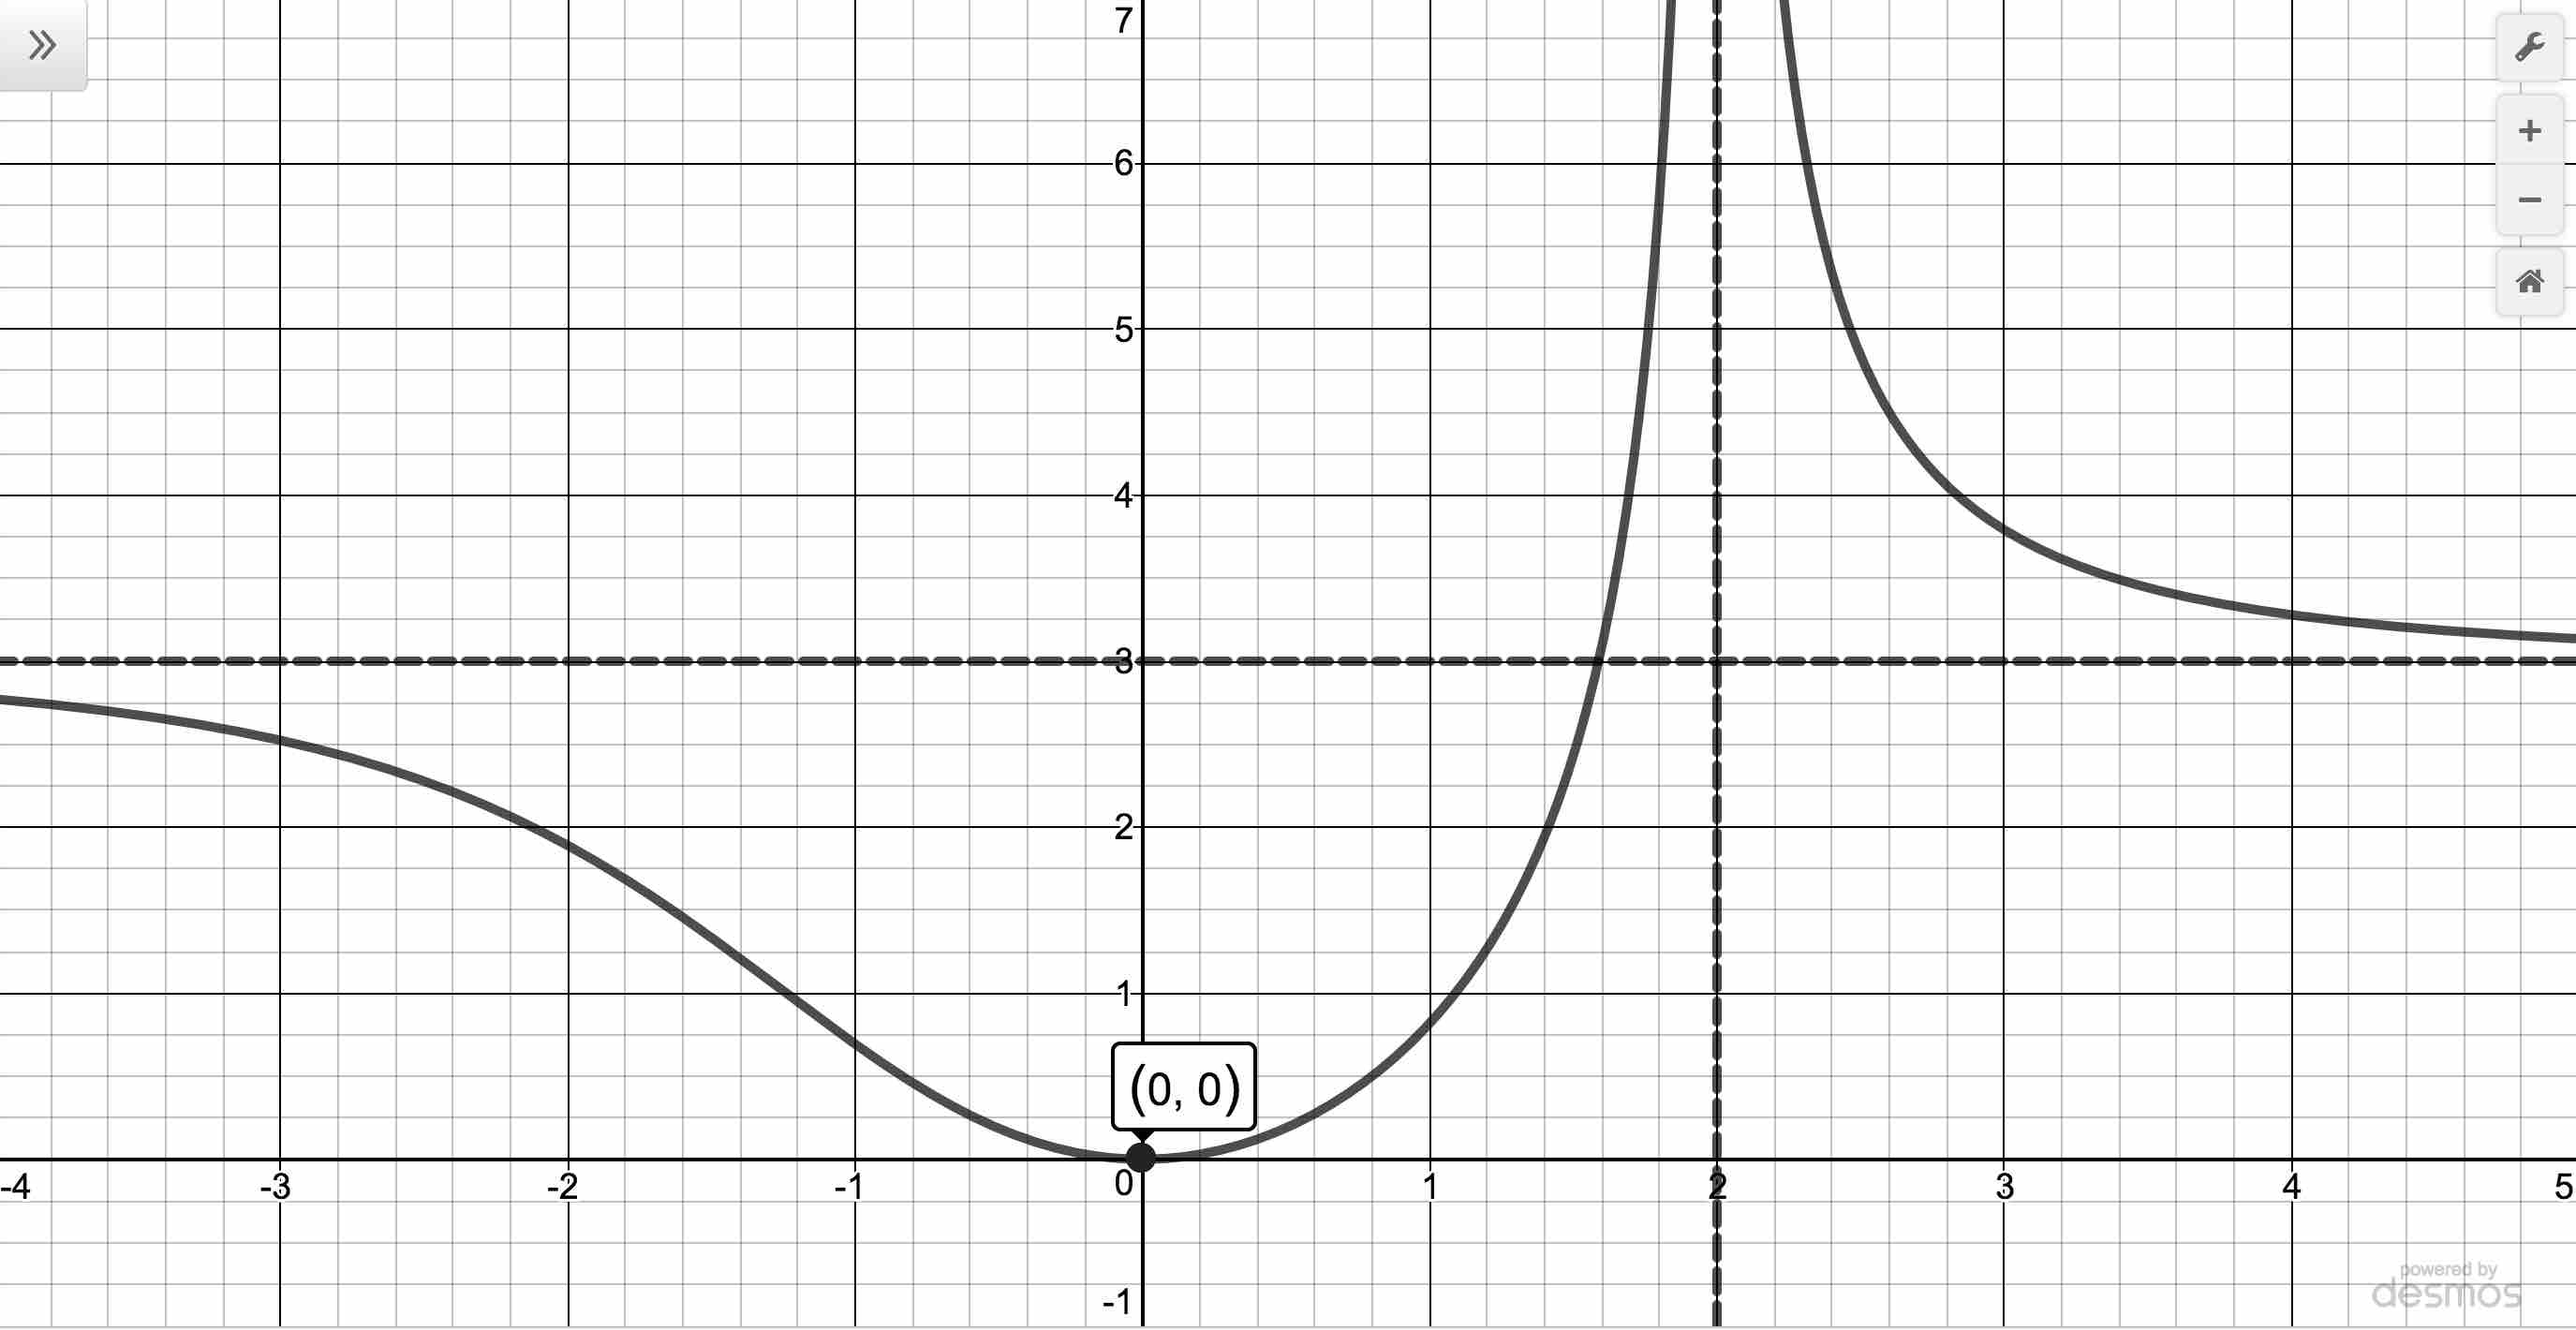
\includegraphics[width=3in]{./PowerFunctionsGraphics/RationalExpEx01.jpg} &

\begin{mfpic}[20]{-4}{2}{-1}{1}
\arrow \reverse \arrow \polyline{(-4,0),(2,0)}
\xmarks{-2,0}
\tlabel[cc](-3, 0.5){$(+)$}
\tlabel[cc](-2,-0.5){$0$}
\tlabel[cc](-2,0.5){$0$}
\tlabel[cc](-1,0.5){$(+)$}
\tlabel[cc](0,-0.5){$2$}
\tlabel[cc](0,0.5){\textinterrobang}
\tlabel[cc](1,0.5){$(+)$}
\end{mfpic}  \\

The graph of $y=f(x)$  \hspace{0.75in} & Sign Diagram for $f(x)$ \\

\end{tabular}

\end{center} 


\item To find the domain of $g(t) = \frac{ (t^2-4)^{\frac{3}{2}} }{t^2-36}$, we have two issues to address:  the denominator and an even (square) root.  Solving $t^2 - 36 = 0$ gives  two excluded values, $t = \pm 6$.  For the numerator, we may rewrite $(t^2-4)^{\frac{3}{2}} = (\sqrt{t^2-4})^3$, so we require $t^2-4 \geq 0$, or  $t^2 \geq 4$.  Extracting square roots, we have $\sqrt{t^2} \geq \sqrt{4}$ or $|t| \geq 2$ which means $t \leq -2$ or $t \geq 2$.  Taking into account our excluded values $t = \pm 6$, we get  the domain of $g$ is $(-\infty, -6) \cup (-6, -2] \cup [2, 6) \cup (6, \infty)$.

Looking near $t = -6$, we note that as $t \rightarrow -6$, $(t^2-4)^{\frac{3}{2}} \approx 32^{\frac{3}{2}} = 32^{1.5}$, a positive number.  As $t \rightarrow -6^{-}$, $t^2-36 \approx \text{small $(+)$}$, so $g(t) \approx \frac{32^{1.5}}{\text{small$(+)$}} \approx \text{big $(+)$}$.  This suggests $\ds{\lim_{t \rightarrow -6^{-}} g(t) =\infty}$.  On the other hand, as $t \rightarrow -6^{+}$, $t^2 -36 \approx \text{small $(-)$}$, so $g(t) \approx \frac{32^{1.5}}{\text{small$(-)$}} \approx \text{big $(-)$}$, suggesting$\ds{\lim_{t \rightarrow -6^{+}} g(t) = -\infty}$. Similarly, we find as  $\ds{\lim_{t \rightarrow 6^{-}} g(t) = -\infty}$ and as  $\ds{\lim_{t \rightarrow 6^{+}} g(t) = \infty}$.  This suggests we have two vertical asymptotes to the graph of $y = g(t)$:  $t = -6$ and $t = 6$.

To find the $t$-intercepts, we set $g(t) = 0$ and solve $(t^2-4)^{\frac{3}{2}} = 0$. This reduces to $t^2-4 =0$ or $t = \pm 2$.  As these are (just barely!) in the domain of $g$, we have two $t$-intercepts, $(-2,0)$ and $(2,0)$.  The graph of $g$ has no $y$-intercepts, since $0$ is not in the domain of $g$, so $g(0)$ is undefined.

Regarding end behavior, as $t \rightarrow  -\infty$ and $t \rightarrow  \infty$, the $t^2$ in both numerator and denominator dominate the constant terms, so we have \[ g(t) =  \dfrac{ (t^2-4)^{\frac{3}{2}} }{t^2-36} \approx  \dfrac{\left(t^2\right)^{\frac{3}{2}}}{t^2} = \dfrac{\left(\sqrt{t^2} \right)^3}{t^2} = \dfrac{|t|^3}{t^2} = \dfrac{|t| |t|^2}{t^2} = \dfrac{|t| t^2}{t^2} = |t|. \]


This suggests that as $t \rightarrow -\infty$ and $t \rightarrow  \infty$, the graph of $y = g(t)$ resembles $y = |t|$.  Hence, $\ds{\lim_{t \rightarrow   -\infty} g(t) = \infty}$ and $\ds{\lim_{t \rightarrow   \infty} g(t) = \infty}$.  Using the piecewise definition of $|t|$, we have that as $t \rightarrow -\infty$, $g(t) \approx -t$ and as $t \rightarrow \infty$, $g(t) \approx t$.  In other words, the graph of  $y = g(t)$ has \textit{two} slant asymptotes with slopes $\pm 1$. 

Graphing $y=g(t)$ below on the left verifies our analysis.  From the graph, the range appears to be $(-\infty, 0] \cup [14.697, \infty)$.  The points $(-10, 14.697)$ and $(10, 14.697)$ are local minimums.  $g$ appears to be decreasing on  $(-\infty, -10]$, $[2, 6)$, and $(6, 10]$. Likewise, $g$ is increasing on $[-10, -6)$, $(-6, -2]$ and $[10, \infty)$.  The graph of $y=g(t)$ certainly appears to be symmetric about the $y$-axis.  We leave it to the reader to show $g$ is, indeed, an even function.

\enlargethispage{1in}

For the sign diagram for $g(t)$, we note that $g$ has zeros $t = \pm 2$ and is undefined at $t = \pm 6$.  Moreover, there is a gap in the domain for all values in the interval $(-2,2)$, so we excise that portion of the real number line for our discussion.  We find $g(t) > 0$ or $(+)$ on the intervals $(-\infty -6)$ and $(6, \infty)$ while $g(t) < 0$ or $(-)$ on $(-6,-2)$ and $(2, 6)$.  Our sign diagram for $g(t)$ is below on the right.  

\begin{center}

\begin{tabular}{cc}

 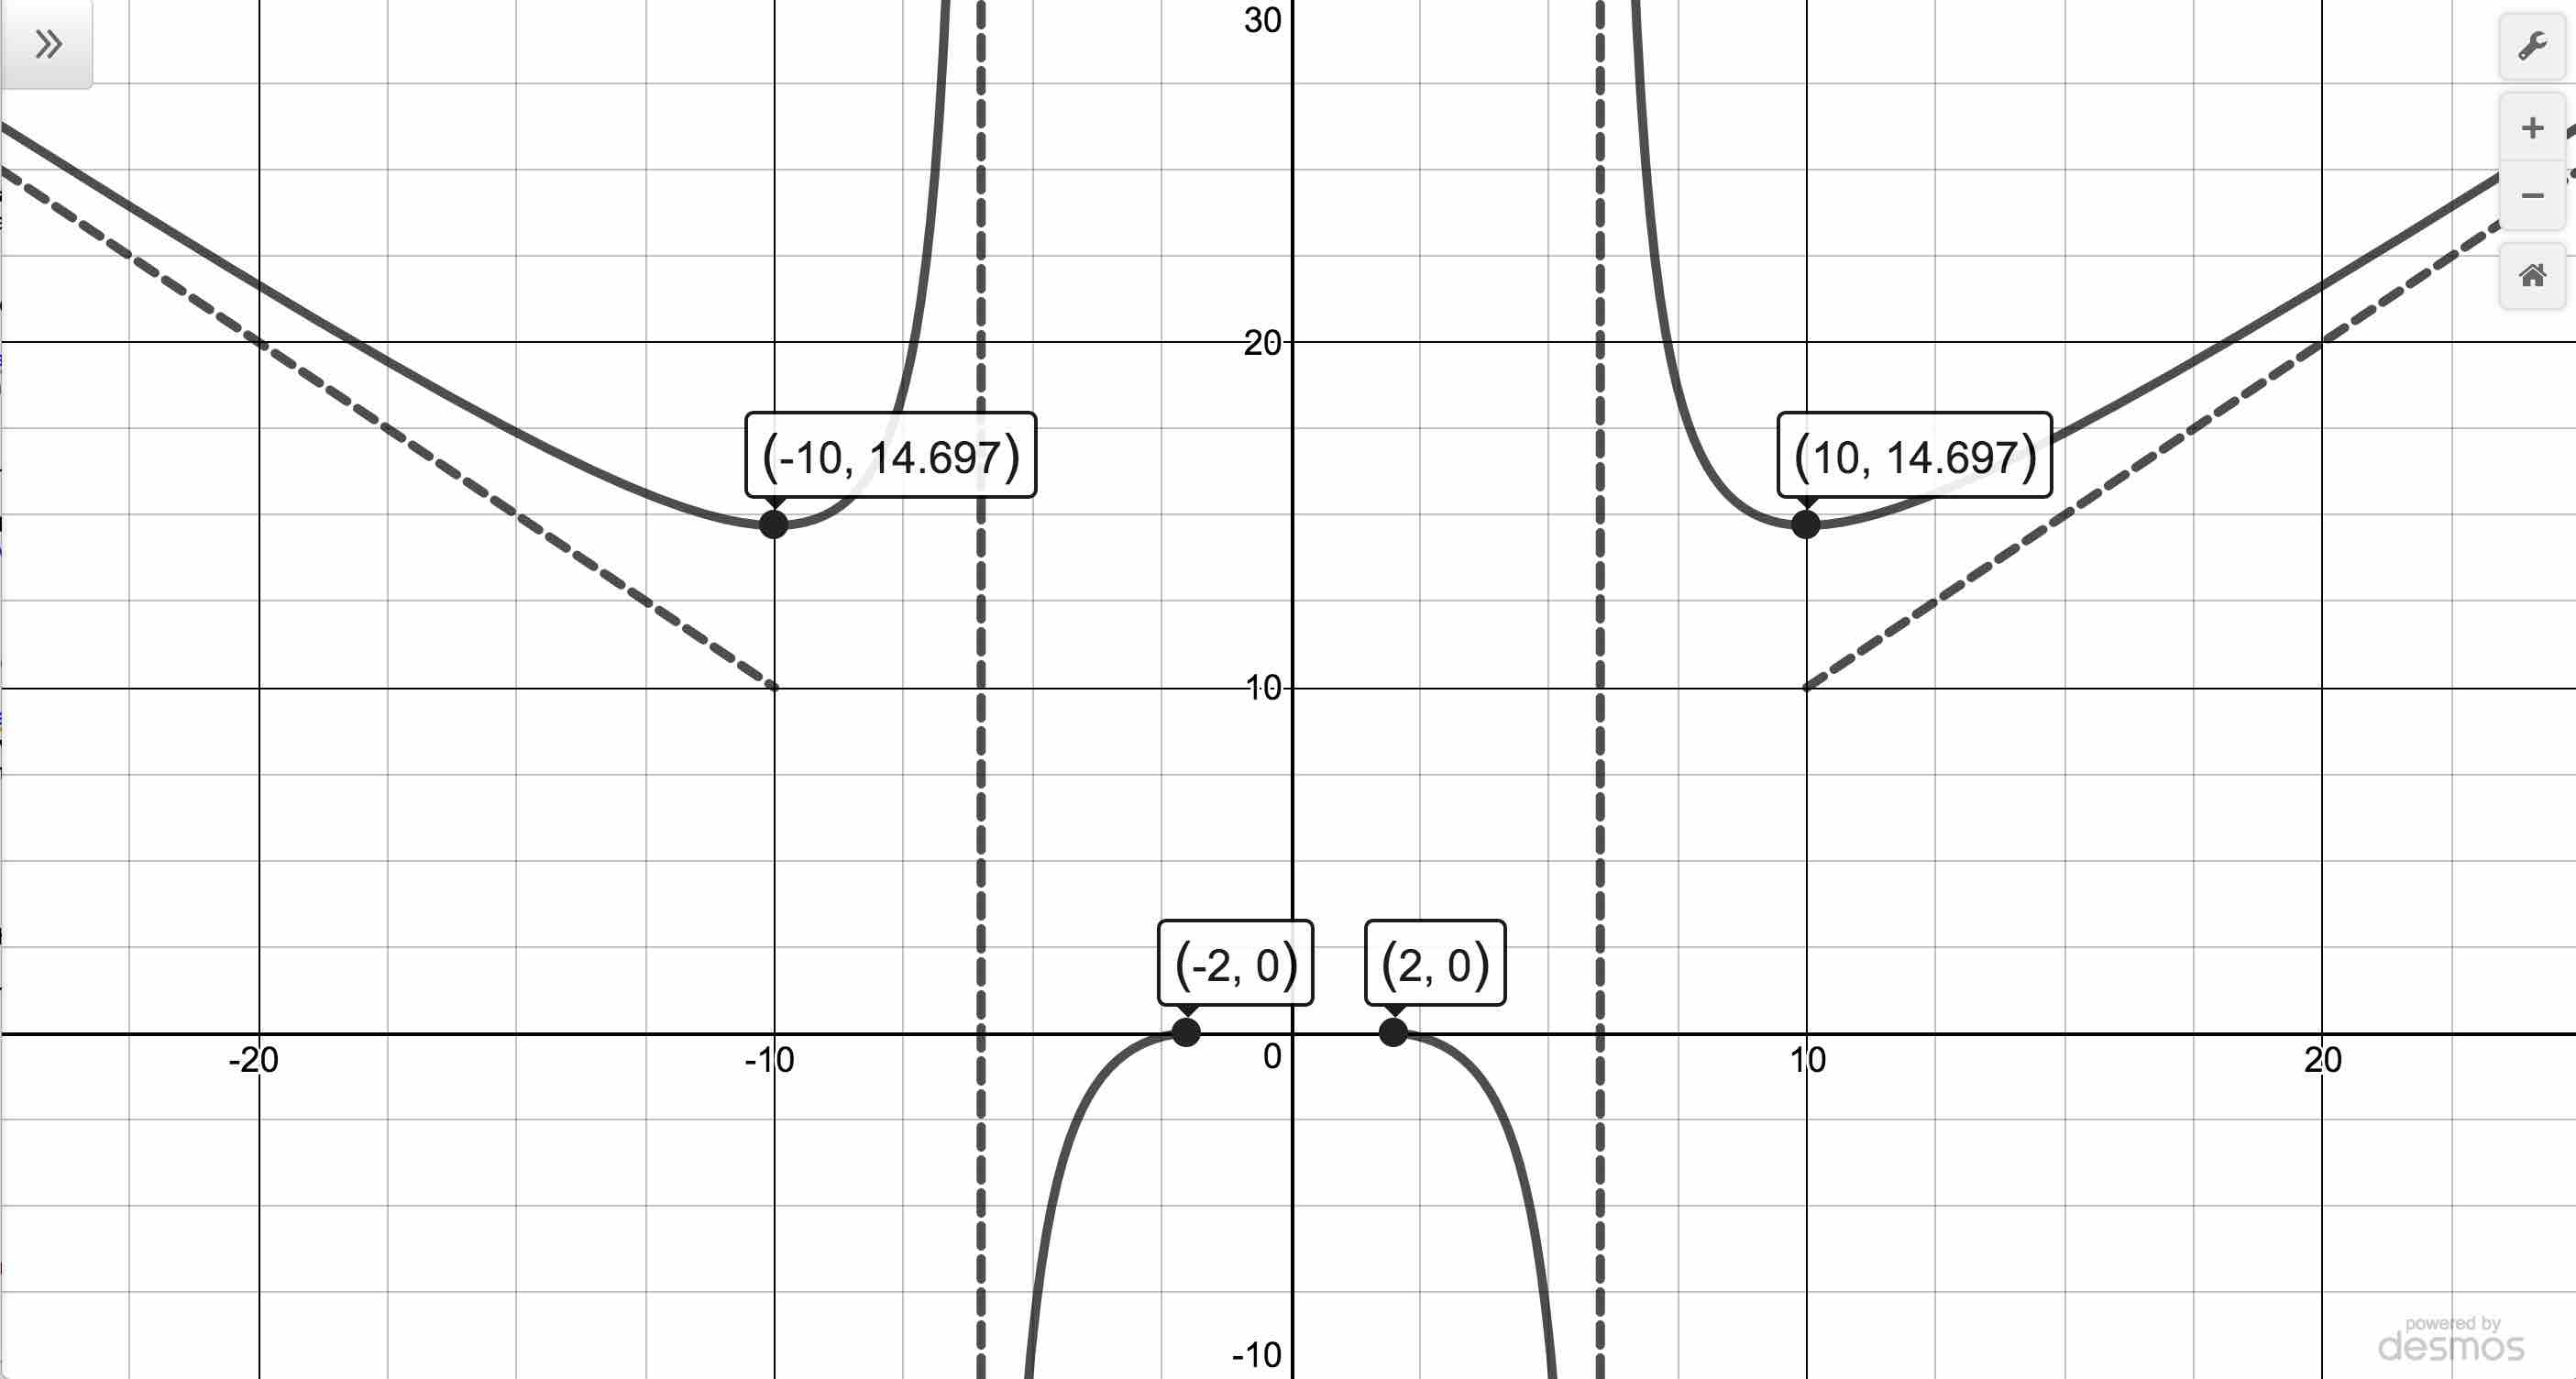
\includegraphics[width=3in]{./PowerFunctionsGraphics/RationalExpEx02.jpg} & 
 
\begin{mfpic}[20][10]{-2}{7}{-1.5}{1.5}
\arrow \polyline{(2,0), (-2,0)}
\arrow \polyline{(3,0), (7,0)}
\xmarks{0, 2, 3, 5}
\tlabel[cc](-1,1){$(+)$}
\tlabel[cc](0,-1){$-6 \hspace{7pt}$}
\tlabel[cc](0,1){\textinterrobang}
\tlabel[cc](1,1){$(-)$}
\tlabel[cc](2,-1){$-2 \hspace{7pt}$}
\tlabel[cc](2,1){$0$}
\tlabel[cc](3,-1){$2$}
\tlabel[cc](3,1){$0$}
\tlabel[cc](4,1){$(-)$}
\tlabel[cc](5,-1){$6$}
\tlabel[cc](5,1){\textinterrobang}
\tlabel[cc](6,1){$(+)$}

\end{mfpic} \\

The graph of $y=g(t)$  \hspace{0.75in} &Sign Diagram for $g(t)$ \\

\end{tabular}

\end{center} 

\qed

\end{enumerate}

\end{example}

\subsection{Real Number Exponents}

We wish now to extend the concept of `exponent' from rational to all real numbers which means we need to discuss how to interpret an irrational exponent.  Once again, the notions presented here are best discussed using the language of Calculus or Analysis, but we nevertheless do what we can with the notions we have.  

Consider  the wildly famous irrational number $\pi$.  The number $\pi$ is defined geometrically as the ratio of the circumference of a circle to that circle's diameter.\footnote{This works for each and every circle, by the way, regardless of how large or small the circle is!} The reason we use the \textit{symbol} `$\pi$' instead of any numerical expression is that $\pi$ is an irrational number, and, as such, its decimal representation neither terminates nor repeats.  Hence we \textit{approximate} $\pi$ as $\pi \approx 3.14$ or $\pi \approx 3.14159265$.  No matter how many digits we write, however, what we have is a \textit{rational number} approximation of $\pi$. 


The good news is we can approximate $\pi$ to any desired accuracy using rational numbers by taking enough digits, so while we'll never `reach' the \textit{exact} value of $\pi$ with rational numbers, we can get \textit{as close as we like} to $\pi$ using rational numbers.  That being said, we assume $\pi$ exists on the real number line, despite the fact the list of digits to pinpoint its location is, in some sense, infinite.

We take this tack  when defining the value of a number raised to an irrational exponent.  Consider, for instance, $2^{\pi}$.  We can compute $2^3 = 8$, $2^{3.1} = 2^{\frac{31}{10}} = \sqrt[10]{2^{31}} \approx 8.574 $, $2^{3.14} = 2^{\frac{314}{100}} = 2^{\frac{157}{50}} = \sqrt[50]{2^{157}} \approx 8.8512$, and so on, so one way to  \textit{define} $2^{\pi}$ as the unique real number we obtain  as the exponents `approach' $\pi$. 

It is with this understanding that we present the notion of a `power function,' as described in Definition   \ref{powerfunction}:  $f(x) = a x^p$ where $a$ and $p$ are nonzero real number parameters.  Here the exponent $p$ is open to any (nonzero) real number.  Because of how we define real number exponents, if $p$ is irrational, then $ x \geq 0$ to avoid having negatives under even-indexed roots as we go through the approximation process.\footnote{or $x > 0$ if $p$ is negative.} 

In general, real number exponents inherit their properties from rational number exponents.  For instance, Theorem \ref{exponentprops} also holds for all real number exponents and the graphs of power functions inherit their behavior from graphs of rational exponent functions.  More specifically, the graphs of functions of the form $f(x)= x^p$ where $p>0$ all contain the points $(0,0)$ and $(1,1)$.  Moreover, these functions are increasing and their graphs are  concave down if $0<p<1$ and concave up if $p>1$. 


\begin{center}

\begin{mfpic}[17]{-1}{9}{-1}{9}
\axes
\tlabel[cc](9, -0.5){\scriptsize $x$}
\tlabel[cc](0.5, 9){\scriptsize $y$}
\tlabel[cc](5,8){\scriptsize $p>1$, concave up}
\tlabel[cc](6,1.5){\scriptsize $0<p<1$, concave down}
\tlabel[cc](0.5, -0.5){\scriptsize $(0,0)$}
\tlabel[cc](1.75, 0.75){\scriptsize $(1,1)$}
\penwd{1.25pt}
\arrow  \parafcn{0, 3,0.1}{(t**2,t)}
\arrow  \parafcn{0, 3,0.1}{(t,t**2)}
\point[4pt]{(0,0), (1,1)}
\tcaption{\scriptsize $f(x) = x^p$ for varying values of $p$.}

\end{mfpic}

\end{center}

Theorem \ref{linearrationalpowergraphs}  generalizes to real number power functions, so, for instance to graph $F(x) = (x-2)^{\pi}$, one need only start with $y = x^{\pi}$ and shift horizontally two units to the right.  (See the Exercises.)  

We close this section with an application to economics.  According to the \href{http://www.census.gov/library/publications/2016/demo/p60-256.html }{\underline{US Census}}, Table 2, the share of money income (2014-2015) is given in the table below on the left. From these data, we can create a cumulative distribution, $y = L(x)$ called the \index{Lorenz Curve}\textbf{Lorenz Curve}.   

The number $L(x)$ gives the percentage of the total national income earned by the bottom $x$ percent of wage earners, ranked from lowest income to highest income.  Since the population here is separated into `quintiles,' each data point corresponds to $20 \%$ of the population.  So, for example, $L(20)$ is the percentage of money income earned by the lowest $20 \%$ of wage earners.  In this case, we see $L(20) = 3.1$.  The number  $L(40)$ is the percentage of the money income earned by the bottom $40 \%$ of wage earners - so this includes not only the money from the Second Quintile, but also the Lowest Quintile:  $L(40) = 8.2 + L(20) = 8.2 +  3.1 = 11.3$.  Likewise, $L(60)$ is the total income share of the bottom $60 \%$ of wage earners which includes the income from the Middle, Second, and Lowest Quintiles:  $L(60) = 14.3 + L(40) = 14.3 + (8.2+3.1) = 25.6$.  

Continuing in this manner, we get $L(80) = 48.8$ and $L(100) = 100$, which is what we would expect:  $100 \%$ of the income is earned by $100 \%$ of the population.  We summarize these findings below  on the right.

\smallskip

\begin{tabular}{cc}

$ \begin{array}{cc}

\text{\small Portion of Population} & \text{ \small Percent of Money Income} \\

\text{\small Lowest Quintile} & \text{\small  3.1} \\

\text{\small Second Quintile} &\text{\small   8.2}  \\

\text{\small Middle Quintile} &  \text{\small 14.3}  \\

\text{\small Fourth Quintile} &  \text{\small  23.2}  \\

\text{\small Highest Quintile} &   \text{\small 51.2 } \\

\end{array} $
&

$ \begin{array}{cc}

\text{\small percent wage earners, $x$} & \text{\small percent income, $L(x)$} \\

\text{\small  20} & \text{\small 3.1}\\

\text{\small 40}  & \text{\small 11.3}  \\

\text{\small 60}  & \text{\small 25.6}  \\

\text{\small 80 }&   \text{\small 48.8}  \\

\text{\small 100}  &  \text{\small 100}  \\

\end{array} $


\end{tabular}

\enlargethispage{1in}

\begin{example} \label{LorenzEx}  $~$

\begin{enumerate}

\item Find power function to model the Lorenz Curve: $L(x) = ax^p$.  Comment on the goodness of fit.  

\item Find and interpret $L(90)$.

\end{enumerate}

{\bf Solution.}  

\begin{enumerate}

\item Using \href{https://www.desmos.com/}{\underline{desmos}}, we get $L(x) = 0.00027901x^{2.7738}$ with $R^2 = 0.993$, indicating a pretty good fit.  

\begin{center}

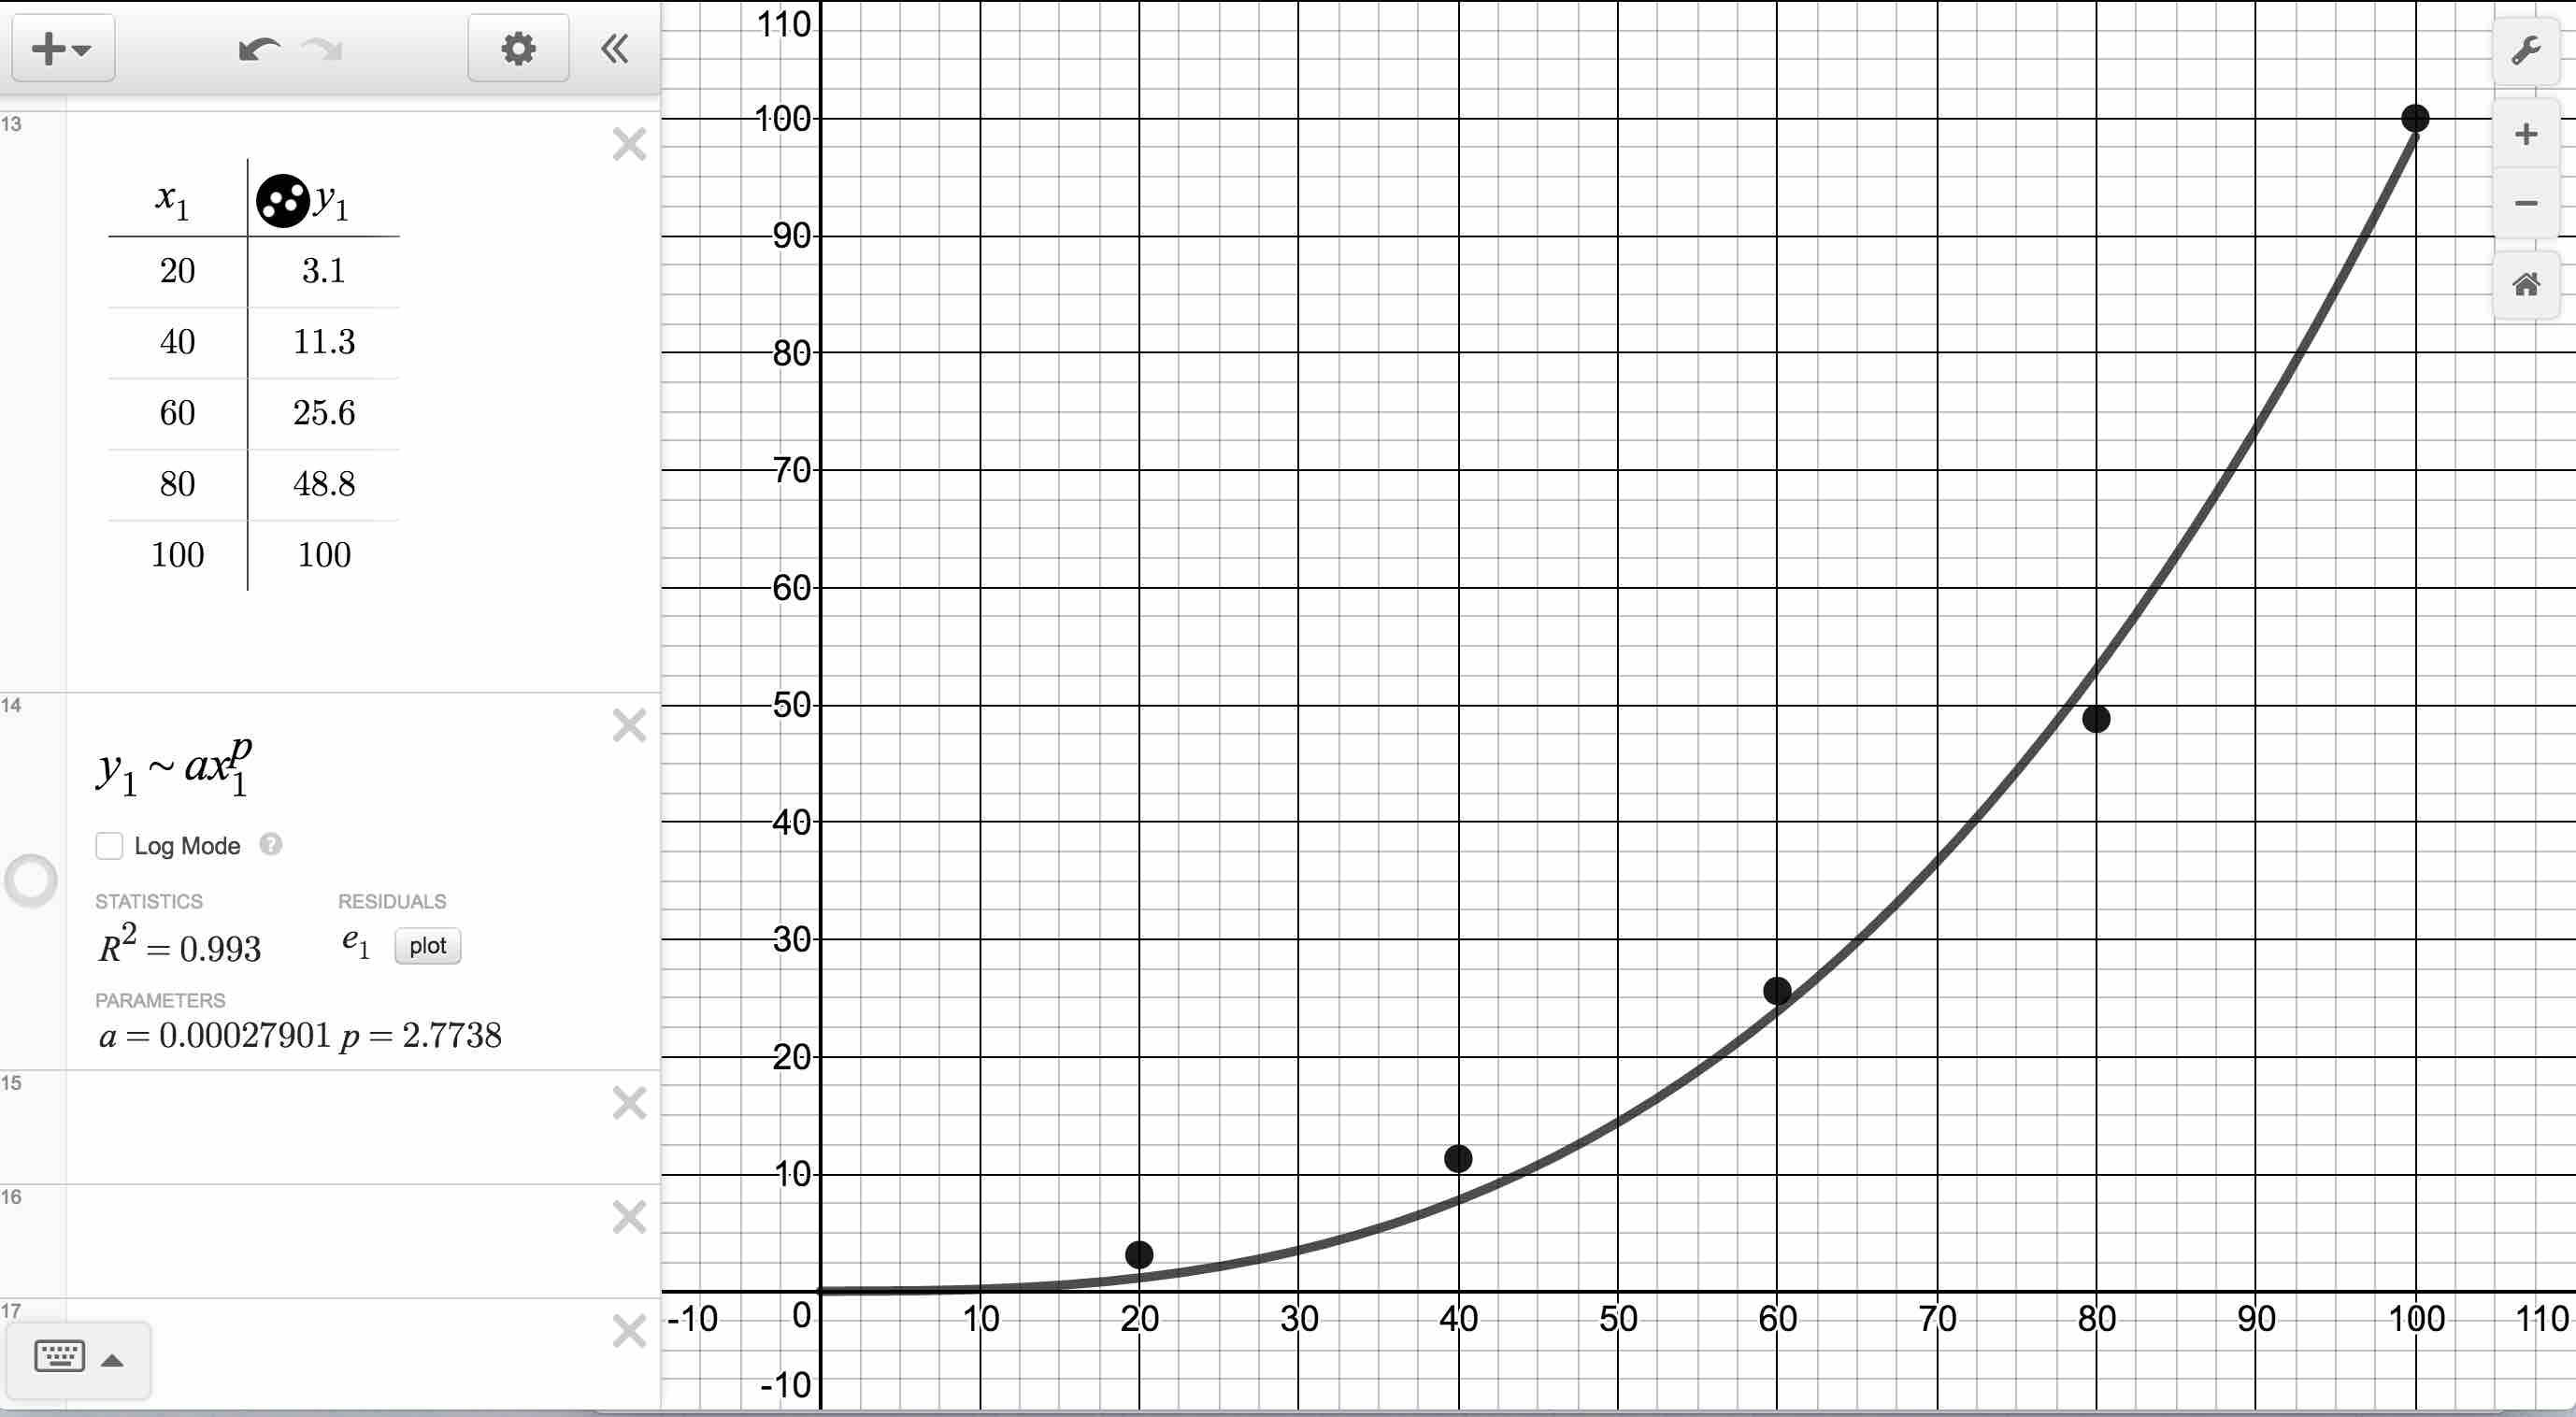
\includegraphics[width=3.5in]{./PowerFunctionsGraphics/LorenzEx.jpg}

\end{center}


\item We compute $L(90) = 0.00027901(90)^{2.7738} \approx 73.5$ meaning that the bottom $90 \%$ of the wage earners brought home $73.5 \%$ of the total income.  Said differently, the top $10 \%$ of wage earners made over $25 \%$ of the total national income.  \qed


\end{enumerate}


 
\end{example}

\newpage

\subsection{Exercises}

%% SKIPPED %% In Exercises \ref{powergraphexfirst} - \ref{powergraphexlast}, use the given graphs along with Theorem \ref{linearrationalpowergraphs} to graph the given function.  Track at least two points and state the domain and range using interval notation.

\begin{center}

\begin{multicols}{2}

\begin{mfpic}[20]{-4}{4}{-1}{4}
\axes
\tlabel[cc](4, -0.5){\scriptsize $x$}
\tlabel[cc](0.5, 4){\scriptsize $y$}
\tlabel[cc](1.75,0.75){\scriptsize $(1,1)$}
\tlabel[cc](-1.75,0.75){\scriptsize $(-1,1)$}
\tlabel[cc](0.5,-0.5){\scriptsize $(0,0)$}
\penwd{1.25pt}
\arrow \reverse \arrow \parafcn{-1.5, 1.5,0.1}{(t**3,t**2)}
\point[4pt]{(-1,1), (0,0), (1,1)}
\tcaption{$f(x)=x^{\frac{2}{3}}$}
\end{mfpic}



\begin{mfpic}[20]{-4}{4}{-1}{4}
\axes
\tlabel[cc](4, -0.5){\scriptsize $t$}
\tlabel[cc](0.5, 4){\scriptsize $y$}
\tlabel[cc](2,1){\scriptsize $(1,1)$}
\tlabel[cc](0.5,-0.5){\scriptsize $(0,0)$}
\penwd{1.25pt}
\arrow  \function{0, 1.5,0.1}{x**3.14}
\point[4pt]{(0,0), (1,1)}
\tcaption{$g(t)=t^{\pi}$ \vphantom{{$f(x)=x^{\frac{2}{3}}$}}}
\end{mfpic}

\end{multicols}
\end{center}

\begin{multicols}{2}
\begin{enumerate}

\item $F(x) = (x-2)^{\frac{2}{3}}-1$ \label{powergraphexfirst}
\item $G(t) = (t+3)^{\pi} +1$

\setcounter{HW}{\value{enumi}}
\end{enumerate}
\end{multicols}

\begin{multicols}{2}
\begin{enumerate}
\setcounter{enumi}{\value{HW}}
\item $F(x) = 3-x^{\frac{2}{3}}$ 
\item $G(t) = (1-t)^{\pi}-2$  \vphantom{$F(x) = 3-x^{\frac{2}{3}}$ }

\setcounter{HW}{\value{enumi}}
\end{enumerate}
\end{multicols}


\begin{multicols}{2}
\begin{enumerate}
\setcounter{enumi}{\value{HW}}

\item $F(x) =(2x+5)^{\frac{2}{3}}+1$ \vphantom{$G(t) = \left( \dfrac{t+3}{2}\right)^{\pi}-1$}
\item $G(t) = \left( \dfrac{t+3}{2}\right)^{\pi}-1$ \label{powergraphexlast}
\setcounter{HW}{\value{enumi}}
\end{enumerate}
\end{multicols}

In Exercises \ref{findformulaforpowergraphfirst} - \ref{findformulaforpowergraphlast}, find a formula for each function below in the form $F(x) = a(bx-h)^{\frac{2}{3}}+k$.

\smallskip

\textbf{NOTE:}  There may be more than one solution!

\begin{multicols}{2}

\begin{enumerate}
\setcounter{enumi}{\value{HW}}

\item $~$ \label{findformulaforpowergraphfirst}  $y=F(x)$ %$F(x) = 2(x-1)^{\frac{2}{3}}-2$

\begin{mfpic}[20]{-4}{4}{-4}{4}
\axes
\tlabel[cc](4, -0.5){\scriptsize $x$}
\tlabel[cc](0.5, 4){\scriptsize $y$}
\tlabel[cc](1, -2.5){\scriptsize $(1,-2)$}
\tlabel[cc](2.5,-0.5){\scriptsize $(2,0)$}
\tlabel[cc](-0.5,-0.5){\scriptsize $(0,0)$}
\penwd{1.25pt}
\arrow \reverse \arrow \parafcn{-1.5, 1.5,0.1}{((t**3)+1,(2*(t**2))-2)}
\point[4pt]{(0,0), (1,-2), (2,0)}
\end{mfpic}
 



\item $~$ \label{findformulaforpowergraphlast} $y = F(x)$ %$F(x) =-(x+1)^{\frac{2}{3}} + 4$

\begin{mfpic}[10][20]{-10}{10}{-2}{6}
\axes
\tlabel[cc](10, -0.5){\scriptsize $x$}
\tlabel[cc](0.5, 6){\scriptsize $y$}
\tlabel[cc](-10, 0.5){\scriptsize $(-9,0)$}
\tlabel[cc](-1.5,4.5){\scriptsize $(-1,4)$}
\tlabel[cc](1.5,3){\scriptsize $(0,3)$}
\tlabel[cc](7,0.5){\scriptsize $(6,0)$}
\penwd{1.25pt}
\arrow \reverse \arrow \parafcn{-2.15,2.15 ,0.1}{((t**3)-1,4-(t**2))}
\point[4pt]{(-9,0), (7,0), (0,3), (-1,4)}
\end{mfpic}
 

\setcounter{HW}{\value{enumi}}

\end{enumerate}

\end{multicols}
\newpage

For each function in Exercises \ref{powerfcngraphexfirst} - \ref{powerfcngraphexlast} below 

\begin{itemize}

\item Analytically:

\begin{multicols}{3}

\begin{itemize}

\item find the domain.

\item find the axis intercepts.

\item analyze the end behavior.

\end{itemize}

\end{multicols}

\item Graph the function with help from a graphing utility and determine:

\begin{multicols}{2}

\begin{itemize}

\item  the range.

\item the local extrema, if they exist.

\end{itemize}

\end{multicols}

\begin{multicols}{2}

\begin{itemize}

\item intervals of increase/decrease.

\item any `unusual steepness' or `local' verticality.

\end{itemize}

\end{multicols}

\begin{multicols}{2}

\begin{itemize}

\item  vertical asymptotes.

\item  horizontal / slant asymptotes.

\end{itemize}

\end{multicols}

\item Construct a sign diagram for each function using the intercepts and graph.

\item  Comment on any observed symmetry.


\end{itemize}


\begin{multicols}{2}
\begin{enumerate}
\setcounter{enumi}{\value{HW}}

\item $f(x) = x^{\frac{2}{3}}(x - 7)^{\frac{1}{3}}$  \label{powerfcngraphexfirst}
\item $f(x) = x^{\frac{3}{2}}(x - 7)^{\frac{1}{3}}$ 


\setcounter{HW}{\value{enumi}}
\end{enumerate}
\end{multicols}

\begin{multicols}{2}
\begin{enumerate}
\setcounter{enumi}{\value{HW}}

\item $g(t) = 2t(t+3)^{-\frac{1}{3}}$ 
\item $g(t) = t^{\frac{3}{2}}(t-2)^{-\frac{1}{2}}$ 


\setcounter{HW}{\value{enumi}}
\end{enumerate}
\end{multicols}

\begin{multicols}{2}
\begin{enumerate}
\setcounter{enumi}{\value{HW}}

\item $f(x) = x^{0.4} (3-x)^{0.6}$ 
\item $f(x) = x^{0.5} (3-x)^{0.5}$ 


\setcounter{HW}{\value{enumi}}
\end{enumerate}
\end{multicols}

\begin{multicols}{2}
\begin{enumerate}
\setcounter{enumi}{\value{HW}}

\item $g(t) = 4t (9-t^2)^{-\sqrt{2}}$ 
\item $g(t) = 3(t^2+1)^{-\pi}$  \label{powerfcngraphexlast}


\setcounter{HW}{\value{enumi}}
\end{enumerate}
\end{multicols}

\begin{enumerate}
\setcounter{enumi}{\value{HW}}

\item \label{powerarcexercise}For each function $f(x)$ listed below, compute the average rate of change over the indicated interval.\footnote{See Definition \ref{arc} in Section \ref{AverageRateofChange} for a review of this concept, as needed.}  What trends do you observe?  How do your answers manifest themselves graphically?  Compare the results of this exercise with those of Exercise \ref{monomialarcexercise} in Section \ref{GraphsofPolynomials} and Exercise \ref{laurentarcexercise} in Section \ref{IntroRational}

\[ \begin{array}{|r||c|c|c|c|}  \hline

 f(x) &  [0.9, 1.1] & [0.99, 1.01] &[0.999, 1.001] & [0.9999, 1.0001]  \\ \hline
 x^{\frac{1}{2}} &&&&  \\  \hline
 x^{\frac{2}{3}} &&&&  \\ \hline
 x^{-0.23} &&&&   \\  \hline
 x^{\pi}  &&&&   \\  \hline

\end{array} \]

\item \label{WindChillTemperature} The \href{http://www.nws.noaa.gov/om/windchill/windchillglossary.shtml}{\underline{National Weather Service}} uses the following formula to calculate the wind chill: \[ W = 35.74 + 0.6215 \, T_{a} - 35.75\, V^{0.16} + 0.4275 \, T_{a} \, V^{0.16}  \] where $W$ is the wind chill temperature in $^{\circ}$F, $T_{a}$ is the air temperature in $^{\circ}$F, and  $V$ is the wind speed in miles per hour.  Note that $W$ is defined only for air temperatures at or lower than $50^{\circ}$F and wind speeds above $3$ miles per hour.

\begin{enumerate}

\item  Suppose the air temperature is $42^{\circ}$ and the wind speed is $7$ miles per hour. Find the wind chill temperature.  Round your answer to two decimal places.

\item  Suppose the air temperature is $37^{\circ}$F and the wind chill temperature is $30^{\circ}$F.  Find the wind speed.  Round your answer to two decimal places. 

\end{enumerate}

\item  As a follow-up to Exercise \ref{WindChillTemperature}, suppose the air temperature is $28^{\circ}$F.  

\begin{enumerate}

\item Use the formula from Exercise \ref{WindChillTemperature} to find an expression for the wind chill temperature as a function of the wind speed, $W(V)$.  

\item  \label{WindChill0} Solve $W(V) = 0$, round your answer to two decimal places,  and interpret.  

\item  Graph the function $W$ using a graphing utility and check your answer to part \ref{WindChill0}. 


\end{enumerate}


\item \label{pursuitfurther} Suppose Fritzy the Fox, positioned at a point $(x,y)$ in the first quadrant, spots Chewbacca the Bunny at $(0,0)$.   Chewbacca begins to run along a fence (the positive $y$-axis) towards his warren.  Fritzy, of course, takes chase and constantly adjusts his direction so that he is always running directly at Chewbacca.  If Chewbacca's speed is $v_{\mbox{\tiny$1$}}$ and  Fritzy's speed is $v_{\mbox{\tiny$2$}}$, the path Fritzy will take to intercept Chewbacca, provided $v_{\mbox{\tiny$2$}}$ is directly proportional to, but not equal to, $v_{\mbox{\tiny$1$}}$ is modeled by

\[ y = \dfrac{1}{2} \left(\dfrac{x^{1+ v_{1}/v_{2}}}{1+v_{\mbox{\tiny$1$}}/v_{\mbox{\tiny$2$}}}- \dfrac{x^{1-v_{\mbox{\tiny$1$}}/v_{\mbox{\tiny$2$}}}}{1-v_{\mbox{\tiny$1$}}/v_{\mbox{\tiny$2$}}}\right) + \dfrac{v_{\mbox{\tiny$1$}} v_{\mbox{\tiny$2$}}}{v_{\mbox{\tiny$2$}}^2-v_{\mbox{\tiny$1$}}^2} \]

\begin{enumerate}

\item  Determine the path that Fritzy will take if he runs exactly twice as fast as Chewbacca;  that is, $v_{\mbox{\tiny$2$}} = 2v_{\mbox{\tiny$1$}}$. Use your calculator to graph this path for $x \geq 0$.  What is the significance of the $y$-intercept of the graph?

\item  Determine the path Fritzy will take if Chewbacca runs exactly twice as fast as he does;  that is, $v_{\mbox{\tiny$1$}} = 2v_{\mbox{\tiny$2$}}$.  Use a graphing utility to graph this path for $x > 0$.  Describe the behavior of $y$ as $x \rightarrow 0^{+}$ and interpret this physically.

\item  With the help of your classmates, generalize parts (a) and (b) to two cases:  $v_{\mbox{\tiny$2$}} > v_{\mbox{\tiny$1$}}$ and $v_{\mbox{\tiny$2$}} < v_{\mbox{\tiny$1$}}$.   We will discuss the case of $v_{\mbox{\tiny$1$}} = v_{\mbox{\tiny$2$}}$ in Exercise \ref{pursuitlog} in Section \ref{ExpLogApplications}.

\end{enumerate}

\setcounter{HW}{\value{enumi}}
\end{enumerate}

\newpage

\subsection{Answers}

\begin{multicols}{2}
\begin{enumerate}

\item  $F(x) = (x-2)^{\frac{2}{3}}-1$ \\

\begin{mfpic}[20]{-2}{6}{-2}{3}
\axes
\tlabel[cc](6, -0.5){\scriptsize $x$}
\tlabel[cc](0.25, 3){\scriptsize $y$}
\tlabel[cc](3.5,-0.5){\scriptsize $(3,0)$}
\tlabel[cc](0.5,-0.5){\scriptsize $(1,0)$}
\tlabel[cc](2,-1.5){\scriptsize $(2,-1)$}
\penwd{1.25pt}
\arrow \reverse \arrow \parafcn{-1.5, 1.5,0.1}{(t**3+2,t**2-1)}
\point[4pt]{(1,0), (2,-1), (3,0)}
\tcaption{Domain:  $(-\infty, \infty)$, Range:  $[-1, \infty)$}
\end{mfpic}


\columnbreak


\item $G(t) = (t+3)^{\pi} +1$ \vphantom{$F(x) = (x-2)^{\frac{2}{3}}-1$}\\

\begin{mfpic}[20]{-7}{1}{0}{5}
\axes
\tlabel[cc](1, -0.5){\scriptsize $t$}
\tlabel[cc](0.5, 5){\scriptsize $y$}
\tlabel[cc](-1,2){\scriptsize $(-2,2)$}
\tlabel[cc](-2.5,0.5){\scriptsize $(-3,1)$}
\penwd{1.25pt}
\arrow  \function{-3,-1.5,0.1}{((x+3)**3.14)+1}
\point[4pt]{(-3,1), (-2,2)}
\tcaption{Domain:  $[-3, \infty)$, Range:  $[1, \infty)$}
\end{mfpic}


\setcounter{HW}{\value{enumi}}
\end{enumerate}
\end{multicols}

\begin{multicols}{2}
\begin{enumerate}
\setcounter{enumi}{\value{HW}}
\item  $F(x) = 3-x^{\frac{2}{3}} = (-1)x^{\frac{2}{3}} + 3$  \\

\begin{mfpic}[20]{-4}{4}{-1}{4}
\axes
\tlabel[cc](4, -0.5){\scriptsize $x$}
\tlabel[cc](0.5, 4){\scriptsize $y$}
\tlabel[cc](1.5,2.25){\scriptsize $(1,2)$}
\tlabel[cc](-1.75,2.25){\scriptsize $(-1,2)$}
\tlabel[cc](0.75,3){\scriptsize $(0,3)$}
\penwd{1.25pt}
\arrow \reverse \arrow \parafcn{-1.5, 1.5,0.1}{(t**3,3-(t**2))}
\point[4pt]{(-1,2), (0,3), (1,2)}
\tcaption{Domain: $(-\infty, \infty)$, Range: $(-\infty,3]$} 
\end{mfpic}


\columnbreak


\item  $G(t) = (1-t)^{\pi}-2 = ((-1)t+1)^{\pi}-2$  \vphantom{$F(x) = 3-x^{\frac{2}{3}}$} \\

\begin{mfpic}[20]{-4}{4}{-3}{2}
\axes
\tlabel[cc](4, -0.5){\scriptsize $t$}
\tlabel[cc](0.5, 2){\scriptsize $y$}
\tlabel[cc](2,-2){\scriptsize $(1,-2)$}
\tlabel[cc](0.75,-1){\scriptsize $(0,-1)$}
\penwd{1.25pt}
\arrow  \reverse \function{-0.5, 1,0.1}{((1-x)**3.14)-2}
\point[4pt]{(0,-1), (1,-2)}
\tcaption{Domain:  $(-\infty, 1]$, Range: $[-2, \infty)$}
\end{mfpic}

\setcounter{HW}{\value{enumi}}
\end{enumerate}
\end{multicols}

\begin{multicols}{2}
\begin{enumerate}
\setcounter{enumi}{\value{HW}}
\item  $F(x) =(2x+5)^{\frac{2}{3}}+1$ \vphantom{$G(t) = \left( \dfrac{t+3}{2}\right)^{\pi}-1$}  \\

\begin{mfpic}[20]{-6.5}{1.5}{-1}{4}
\axes
\tlabel[cc](1.5, -0.5){\scriptsize $x$}
\tlabel[cc](0.5, 4){\scriptsize $y$}
\tlabel[cc](-4,1.75){\scriptsize $(-3,2)$}
\tlabel[cc](-2.5,0.5){\scriptsize $\left(-\frac{5}{2},1 \right)$}
\tlabel[cc](-1,1.75){\scriptsize $(-2,2)$}
\penwd{1.25pt}
\arrow \reverse \arrow \parafcn{-1.6, 1.6,0.1}{( 0.5*( (t**3)-5),(t**2)+1)}
\point[4pt]{(-3,2), (-2.5,1), (-2,2)}
\tcaption{Domain: $(-\infty, \infty)$, Range: $[1, \infty)$}
\end{mfpic}


\columnbreak


\item  $G(t) = \left( \dfrac{t+3}{2}\right)^{\pi}-1= \left( \frac{1}{2} \, t + \frac{3}{2}\right)^{\pi} -1$\\

\begin{mfpic}[20]{-4}{4}{-2}{3}
\axes
\tlabel[cc](4, -0.5){\scriptsize $t$}
\tlabel[cc](0.5, 3){\scriptsize $y$}
\tlabel[cc](-3,-1.5){\scriptsize $(-3,-1)$}
\tlabel[cc](-1.5,0.5){\scriptsize $(-1,0)$}
\penwd{1.25pt}
\arrow  \function{-3, -0.2,0.1}{(((x+3)/2)**3.14)-1}
\point[4pt]{(-3,-1), (-1,0)}
\tcaption{Domain:  $[-3, \infty)$, Range: $[-1, \infty)$}
\end{mfpic}

\setcounter{HW}{\value{enumi}}
\end{enumerate}
\end{multicols}

\begin{multicols}{2}

\begin{enumerate}
\setcounter{enumi}{\value{HW}}

\item One solution is: $F(x) = 2(x-1)^{\frac{2}{3}}-2$

\item  One solution is: $F(x) =-(x+1)^{\frac{2}{3}} + 4$


\setcounter{HW}{\value{enumi}}
\end{enumerate}

\end{multicols}

\newpage

\begin{enumerate}
\setcounter{enumi}{\value{HW}}

\item \begin{multicols}{2} 
$f(x) = x^{\frac{2}{3}}(x - 7)^{\frac{1}{3}}$\\
Domain: $(-\infty, \infty)$\\
Intercepts: $(0,0)$, $(7,0)$\\
Graph: \\

\begin{mfpic}[10]{-4}{10}{-5}{5.5}
\axes
\tlabel[cc](10,-0.5){\scriptsize $x$}
\tlabel[cc](0.5,5.5){\scriptsize $y$}
\tlabel[cc](5,-5){\scriptsize $\approx (4.667, -3.704)$}
\xmarks{-3 step 1 until 9}
\ymarks{-4 step 1 until 5}
\tlpointsep{4pt}
\tiny
\axislabels {x}{{$-3 \hspace{6pt}$} -3, {$-2 \hspace{6pt}$} -2, {$-1 \hspace{6pt}$} -1, {$1$} 1, {$2$} 2, {$3$} 3, {$4$} 4, {$5$} 5, {$6$} 6,  {$8$} 8, {$9$} 9}
\axislabels {y}{{$-4$} -4, {$-3$} -3, {$-2$} -2,  {$1$} 1, {$2$} 2, {$3$} 3, {$4$} 4, {$5$} 5}
\normalsize
\point[4pt]{(0,0), (7,0), (4.667, -3.704)}
\dashed \polyline{(-3, -5.33), (9, 6.67)}
\penwd{1.25pt}
\arrow \reverse \function{-3,0,0.1}{-((x**2)**(1/3))*((7 - x)**(1/3))}
\function{0,7,0.1}{-((x**2)**(1/3))*((7 - x)**(1/3))}
\arrow \function{7,9,0.1}{((x**2)**(1/3))*((x - 7)**(1/3))}
\end{mfpic}

\vfill
\columnbreak

$\ds{\lim_{x \rightarrow - \infty} f(x) = - \infty}$, $\ds{\lim_{x \rightarrow \infty} f(x) = \infty}$\footnote{Using Calculus it can be shown that $y = x - \frac{7}{3}$ is a slant asymptote of this graph.}\\
Range: $(-\infty, \infty)$\\
Local minimum: $\approx (4.667, -3.704)$\\
Local maximum: $(0,0)$ (this is a cusp) \\
Increasing: $(-\infty, 0]$, $\approx [4.667, \infty)$\\
Decreasing: $[0, 4.667]$\\
Unusual steepness at $x = 7$\\

Sign Diagram:\\

\smallskip

\begin{mfpic}[10]{-3}{10}{-2}{2}
\arrow \reverse \arrow \polyline{(-3,0),(10,0)}
\xmarks{0,7}
\tlabel[cc](-1.5,1){$(-)$}
\tlabel[cc](0,-1){$0$}
\tlabel[cc](0,1){$0$}
\tlabel[cc](3.5,1){$(-)$}
\tlabel[cc](7,-1){$7$}
\tlabel[cc](7,1){$0$}
\tlabel[cc](8.5,1){$(+)$}
\end{mfpic}



\end{multicols}

\item \begin{multicols}{2} 
$f(x) = x^{\frac{3}{2}}(x - 7)^{\frac{1}{3}}$\\
Graph: \\
\begin{mfpic}[15][3]{-1}{8.5}{-20}{30}
\axes
\tlabel[cc](8.5,-3){\scriptsize $x$}
\tlabel[cc](0.5,30){\scriptsize $y$}
\tlabel[cc](6,-18){\scriptsize $\approx (5.727, -14.854)$}
\xmarks{1 step 1 until 8}
\ymarks{-15 step 5 until 25}
\tlpointsep{4pt}
\scriptsize
\axislabels {x}{ {$2$} 2, {$3$} 3, {$4$} 4, {$5$} 5, {$6$} 6,  {$8$} 8}
\axislabels {y}{{$-15$} -15, {$-10$} -10, {$-5$} -5, {$5$} 5, {$10$} 10, {$15$} 15, {$20$} 20, {$25$} 25}
\normalsize
\point[4pt]{(0,0), (7,0), (5.727, -14.854)}
\penwd{1.25pt}
\function{0,7,0.1}{-(x**1.5)*((7 - x)**(1/3))}
\arrow \function{7,8.5,0.1}{(x**1.5)*((x - 7)**(1/3))}
\end{mfpic}


\vfill
\columnbreak

Domain: $[0, \infty)$\\
Intercepts: $(0,0)$, $(7,0)$\\
$\ds{\lim_{x \rightarrow \infty} f(x) = \infty}$\\
Range:  $\approx [-14.854, \infty)$\\
Local minimum:  $\approx (5.727, -14.854)$\\
Increasing: $\approx [5.727, \infty)$\\
Decreasing: $\approx [0, 5.727]$\\
Unusual steepness at $x = 7$\\
Sign Diagram:\\

\smallskip

\begin{mfpic}[15]{0}{10}{-1}{1}
\reverse \arrow \polyline{(0,0),(10,0)}
\xmarks{0, 7}
\tlabel[cc](0,-0.5){$0$}
\tlabel[cc](0,0.5){$0$}
\tlabel[cc](3.5, 0.5){$(-)$}
\tlabel[cc](7,-0.5){$7$}
\tlabel[cc](7,0.5){$0$}
\tlabel[cc](8, 0.5){$(+)$}
\end{mfpic}


\end{multicols}

\setcounter{HW}{\value{enumi}}
\end{enumerate}


\begin{enumerate}
\setcounter{enumi}{\value{HW}}

\item \begin{multicols}{2} 
 $g(t) = 2t(t+3)^{-\frac{1}{3}}$ \\
Graph: \\

\begin{mfpic}[10][5]{-10}{5}{-10}{10}
\axes
\tlabel[cc](5,-0.5){\scriptsize $t$}
\tlabel[cc](0.5,10){\scriptsize $y$}
\tlabel[cc](-6,5){\scriptsize $\approx (-4.5, 7.862)$}
\xmarks{-9 step 1 until 4}
\ymarks{-8 step 2 until 8}
\tlpointsep{4pt}
\tiny
\axislabels {x}{{$-9 \hspace{6pt}$} -9, {$-8 \hspace{6pt}$} -8, {$-7 \hspace{6pt}$} -7, {$-6 \hspace{6pt}$} -6, {$-5 \hspace{6pt}$} -5, {$-4 \hspace{6pt}$} -4, {$-3 \hspace{6pt}$} -3, {$-2 \hspace{6pt}$} -2, {$-1 \hspace{6pt}$} -1, {$1$} 1, {$2$} 2, {$3$} 3, {$4$} 4}
\axislabels {y}{ {$-8$} -8,  {$-6$} -6, {$-4$} -4, {$-2$} -2,   {$2$} 2, {$4$} 4,  {$6$} 6,  {$8$} 8}
\normalsize
\dashed \polyline{(-3,-9), (-3, 10)}
\point[4pt]{(0,0), (-4.5, 7.862)}
\penwd{1.25pt}
\arrow \reverse \arrow \function{-9,-3.2,0.1}{-(2*x)/((-x-3)**(1/3))}
\arrow \reverse \function{-2.8,0,0.1}{(2*x)/((x+3)**(1/3))}
\arrow \function{0,5,0.1}{(2*x)/((x+3)**(1/3))}

\end{mfpic}

\vfill
\columnbreak

Domain: $(-\infty, -3) \cup (-3, \infty)$\\
Intercept: $(0,0)$\\
$\ds{\lim_{t \rightarrow -\infty} g(t) = \infty}$\\
$\ds{\lim_{t \rightarrow \infty} g(t) = \infty}$\\
Range: $(-\infty, \infty)$\\
Local minimum: $\approx (-4.5, 7.862)$\\
Increasing: $\approx [-4.5, -3)$, $(-3,\infty)$ \\
Decreasing: $\approx (-\infty, -4.5]$\\
Vertical Asymptote:  $t = -3$\\
Sign Diagram:\\

\smallskip

\begin{mfpic}[10]{-3}{10}{-2}{2}
\arrow \reverse \arrow \polyline{(-3,0),(10,0)}
\xmarks{0,7}
\tlabel[cc](-1.5,1){$(+)$}
\tlabel[cc](0,-1){$-3 \hspace{6pt}$}
\tlabel[cc](0,1){\textinterrobang}
\tlabel[cc](3.5,1){$(-)$}
\tlabel[cc](7,-1){$0$}
\tlabel[cc](7,1){$0$}
\tlabel[cc](8.5,1){$(+)$}
\end{mfpic}



\end{multicols}

\item \begin{multicols}{2} 
$g(t)= t^{\frac{3}{2}}(t-2)^{-\frac{1}{2}}$\\
Domain:  $(2, \infty)$\\
$\ds{\lim_{t \rightarrow \infty} g(t) = \infty}$\\
Graph: \\
\begin{mfpic}[15][10]{-1}{10}{-1}{10}
\axes
\tlabel[cc](10,-0.5){\scriptsize $t$}
\tlabel[cc](0.5,10){\scriptsize $y$}
\xmarks{1 step 1 until 9}
\ymarks{1 step 2 until 9}
\tlpointsep{4pt}
\tiny
\axislabels {x}{{$1$} 1, {$2$} 2, {$3$} 3, {$4$} 4, {$5$} 5, {$6$} 6,  {$7$} 7, {$8$} 8, {$9$} 9}
\axislabels {y}{{$1$} 1,  {$3$} 3, {$5$} 5,  {$7$} 7,  {$9$} 9}
\normalsize
\dashed \polyline{(2,5), (2,9)}
\dashed \polyline{(4,5), (9,10)}
\gclear \tlabelrect(3,4){\scriptsize $\approx (3, 5.196)$}
\point[4pt]{(3, 5.196)}
\penwd{1.25pt}
\arrow \reverse \arrow \function{2.1,8.75,0.1}{(x**1.5)*((x - 2)**(-0.5))}
\end{mfpic}


\vfill
\columnbreak
$\ds{\lim_{t \rightarrow \infty} g(t) = \infty}$\footnote{Using Calculus it can be shown that $y = t+1$ is a slant asymptote of this graph.}\\
Range:  $\approx [5.196, \infty)$\\
Local minimum:  $\approx (3, 5.196)$\\
Increasing: $\approx [3, \infty)$\\
Decreasing: $\approx (2,3]$\\
Vertical asymptote:  $t = 2$\\
Sign Diagram:\\

\smallskip

\begin{mfpic}[15]{0}{10}{-1}{1}
\reverse \arrow \polyline{(0,0),(4,0)}
\xmarks{0}
\tlabel[cc](0,-0.5){$2$}
\tlabel[cc](0,0.5){\textinterrobang}
\tlabel[cc](2, 0.5){$(+)$}
\end{mfpic}


\end{multicols}

\setcounter{HW}{\value{enumi}}
\end{enumerate}



\begin{enumerate}
\setcounter{enumi}{\value{HW}}

\item \begin{multicols}{2} 
 $f(x) = x^{0.4}(3-x)^{0.6}$ \\
Graph: \\
\begin{mfpic}[20]{-2}{5}{-2}{4}
\axes
\tlabel[cc](5,-0.5){\scriptsize $x$}
\tlabel[cc](0.5,4){\scriptsize $y$}
\tlabel[cc](2,2){\scriptsize $\approx (1.2, 1.531)$}
\xmarks{-1 step 1 until 4}
\ymarks{-1 step 1 until 3}
\tlpointsep{4pt}
\tiny
\axislabels {x}{ {$-1 \hspace{6pt}$} -1, {$1$} 1, {$2$} 2,  {$4$} 4}
\axislabels {y}{{$-1$} -1,   {$2$} 2,   {$3$} 3,   {$4$} 4}
\normalsize
%\dashed \polyline{(-3,-9), (-3, 10)}
\point[4pt]{(0,0), (3,0), (1.2, 1.531)}
\penwd{1.25pt}
\function{0,3,0.1}{(x**0.4)*((3-x)**0.6)}

\end{mfpic}

\vfill
\columnbreak


Domain: $[0,3]$\\
Intercepts: $(0,0)$, $(3,0)$\\
Range: $\approx [0, 1.5]$\\
Increasing: $\approx [0, 1.2]$ \\
Decreasing: $\approx [1.2, 3]$\\
Unusual Steepness:\footnote{Note you may need to zoom in to see this.}  $x=0$, $x = 3$\\
Sign Diagram:\\

\smallskip

\begin{mfpic}[10]{-3}{10}{-2}{2}
 \polyline{(0,0),(7,0)}
\xmarks{0,7}
\tlabel[cc](0,-1){$0$}
\tlabel[cc](0,1){$0$}
\tlabel[cc](3.5,1){$(+)$}
\tlabel[cc](7,-1){$3$}
\tlabel[cc](7,1){$0$}
\end{mfpic}




\end{multicols}

\item \begin{multicols}{2} 
 $f(x) = x^{0.5}(3-x)^{0.5}$ \\
Graph: \\
\begin{mfpic}[20]{-2}{5}{-2}{4}
\axes
\tlabel[cc](5,-0.5){\scriptsize $x$}
\tlabel[cc](0.5,4){\scriptsize $y$}
\tlabel[cc](2,2){\scriptsize $\approx (1.5, 1.5)$}
\xmarks{-1 step 1 until 4}
\ymarks{-1 step 1 until 3}
\tlpointsep{4pt}
\tiny
\axislabels {x}{ {$-1 \hspace{6pt}$} -1, {$1$} 1, {$2$} 2,  {$4$} 4}
\axislabels {y}{{$-1$} -1,   {$1$} 1,  {$2$} 2,   {$3$} 3}
\normalsize
\point[4pt]{(0,0), (3,0), (1.5, 1.5)}
\penwd{1.25pt}
\function{0,3,0.1}{(x**0.5)*((3-x)**0.5)}
\end{mfpic}

\vfill
\columnbreak

Domain: $[0,3]$\\
Intercepts: $(0,0)$, $(3,0)$\\
Range: $\approx [0, 1.5]$\\
Increasing: $\approx [0, 1.5]$ \\
Decreasing: $\approx [1.5, 3]$\\
Unusual Steepness:\footnote{Note you may need to zoom in to see this.}  $x=0$, $x = 3$\\
Sign Diagram:\\

\smallskip

\begin{mfpic}[10]{-3}{10}{-2}{2}
 \polyline{(0,0),(7,0)}
\xmarks{0,7}
\tlabel[cc](0,-1){$0$}
\tlabel[cc](0,1){$0$}
\tlabel[cc](3.5,1){$(+)$}
\tlabel[cc](7,-1){$3$}
\tlabel[cc](7,1){$0$}
\end{mfpic}
\end{multicols}
\setcounter{HW}{\value{enumi}}
\end{enumerate}

\newpage

\begin{enumerate}
\setcounter{enumi}{\value{HW}}

\item \begin{multicols}{2} 
$g(t) = 4t (9-t^2)^{-\sqrt{2}}$\\
Graph: \\
\begin{mfpic}[15]{-4}{4}{-3}{3}
\axes
\tlabel[cc](4,-0.5){\scriptsize $t$}
\tlabel[cc](0.5,4){\scriptsize $y$}
\xmarks{-2 step 1 until 2}
\ymarks{-2 step 1 until 2}
\tlpointsep{4pt}
\tiny
\axislabels {x}{ {$-2 \hspace{6pt}$} -2,{$-1 \hspace{6pt}$} -1, {$1$} 1, {$2$} 2}
\axislabels {y}{{$-2$} -2, {$-1$} -1,   {$1$} 1,   {$2$} 2}
\normalsize
\dashed \polyline{(-3,-3), (-3, 3)}
\dashed \polyline{(3,-3), (3, 3)}
\point[4pt]{(0,0)}
\penwd{1.25pt}
\arrow \reverse \arrow  \function{-2.6,2.6,0.1}{4*x/((9-(x**2))**1.414)}
\end{mfpic}

\vfill
\columnbreak
 Domain: $(-3, 3)$\\
Intercepts: $(0,0)$\\
Range: $(-\infty, \infty)$\\
$\ds{\lim_{t \rightarrow -3^{+}} g(t) = -\infty}$, $\ds{\lim_{t \rightarrow 3^{-}} g(t) = \infty}$ \\
Vertical asymptotes:  $t = -3$ and $t = 3$\\
Increasing: $(-3,3)$ \\
Sign Diagram:\\

\smallskip

\begin{mfpic}[10]{-5}{5}{-2}{2}
\polyline{(-5,0),(5,0)}
\xmarks{-5,0,5}
\tlabel[cc](-5,-1){$-3 \hspace{6pt}$}
\tlabel[cc](-5,1){\textinterrobang}
\tlabel[cc](-2.5,1){$(-)$}
\tlabel[cc](0,-1){$0$}
\tlabel[cc](0,1){$0$}
\tlabel[cc](2.5,1){$(+)$}
\tlabel[cc](5,-1){$3$}
\tlabel[cc](5,1){\textinterrobang}
\end{mfpic}

Note:  $g$ is odd

\end{multicols}

\item \begin{multicols}{2} 
$g(t) = 3(t^2+1)^{-\pi}$ \\
Domain: $(-\infty, \infty)$\\
Graph: \\
\begin{mfpic}[20]{-4}{4}{-1}{4}
\axes
\tlabel[cc](4,-0.5){\scriptsize $t$}
\tlabel[cc](0.5,4){\scriptsize $y$}
\xmarks{-3 step 1 until 3}
\ymarks{1 step 1 until 3}
\tlpointsep{4pt}
\tiny
\axislabels {x}{ {$-3 \hspace{6pt}$} -3,{$-2 \hspace{6pt}$} -2,{$-1 \hspace{6pt}$} -1, {$1$} 1, {$2$} 2, {$3$} 3}
\axislabels {y}{ {$1$} 1,   {$2$} 2,   {$3$} 3}
\normalsize
\point[4pt]{(0,3)}
\penwd{1.25pt}
\arrow \reverse \arrow  \function{-3,3,0.1}{3/(((x**2)+1)**3.14)}
\end{mfpic}

\vfill
\columnbreak

Intercept: $(0,3)$\\
$\ds{\lim_{t \rightarrow -\infty} g(t) =0}$ \\
$\ds{\lim_{t \rightarrow \infty} g(t) =0}$ \\
Range: $(0, 3]$\\
Increasing: $(-\infty, 0]$ \\
Decreasing: $[0, \infty)$\\
Horizontal asymptote:  $y =0$\\
Sign Diagram:\\

\vspace*{-0.2in}

\begin{mfpic}[10]{-5}{5}{-2}{2}
 \arrow \reverse \arrow \polyline{(-5,0),(5,0)}

\tlabel[cc](0,1){$(+)$}

\end{mfpic}

Note:  $g$ is even

\end{multicols}
\setcounter{HW}{\value{enumi}}
\end{enumerate}

\begin{enumerate}
\setcounter{enumi}{\value{HW}}

\item As in  Exercise \ref{monomialarcexercise} in Section \ref{GraphsofPolynomials} and Exercise \ref{laurentarcexercise} in Section \ref{IntroRational}, the slopes of these curves near $x = 1$ approach the value of the exponent on $x$.

\[ \begin{array}{|r||c|c|c|c|}  \hline

 f(x) &  [0.9, 1.1] & [0.99, 1.01] &[0.999, 1.001] & [0.9999, 1.0001]  \\ \hline
 x^{\frac{1}{2}} & 0.5006 & \approx \frac{1}{2} & \approx \frac{1}{2} & \approx \frac{1}{2} \\ [5pt] \hline
 x^{\frac{2}{3}} & 0.6672 & 0.6667 & \approx \frac{2}{3} & \approx \frac{2}{3}  \\ [5pt] \hline
 x^{-0.23} & -0.2310 & \approx -0.23 &\approx -0.23 &  \approx -0.23  \\  \hline
 x^{\pi}  &3.1544 & 3.1417 & \approx \pi & \approx \pi   \\  \hline

\end{array} \]

\item

\begin{enumerate}

\item  $W \approx 37.55^{\circ}$F.

\item  $V \approx 9.84$ miles per hour.

\end{enumerate}

\item 

\begin{enumerate}

\item $W(V) = 53.142 - 23.78 V^{0.16}$.  Since we are told in Exercise \ref{WindChillTemperature} that wind chill is only effect for wind speeds of more than 3 miles per hour, we restrict the domain to $V > 3$.

\item $W(V)=0$ when $V \approx 152.29$.  This means, according to the model, for the wind chill temperature to be $0^{\circ}$F, the wind speed needs to be $152.29$ miles per hour.

\newpage

\item The graph of $y = W(V)$ is below.  \\

\centerline{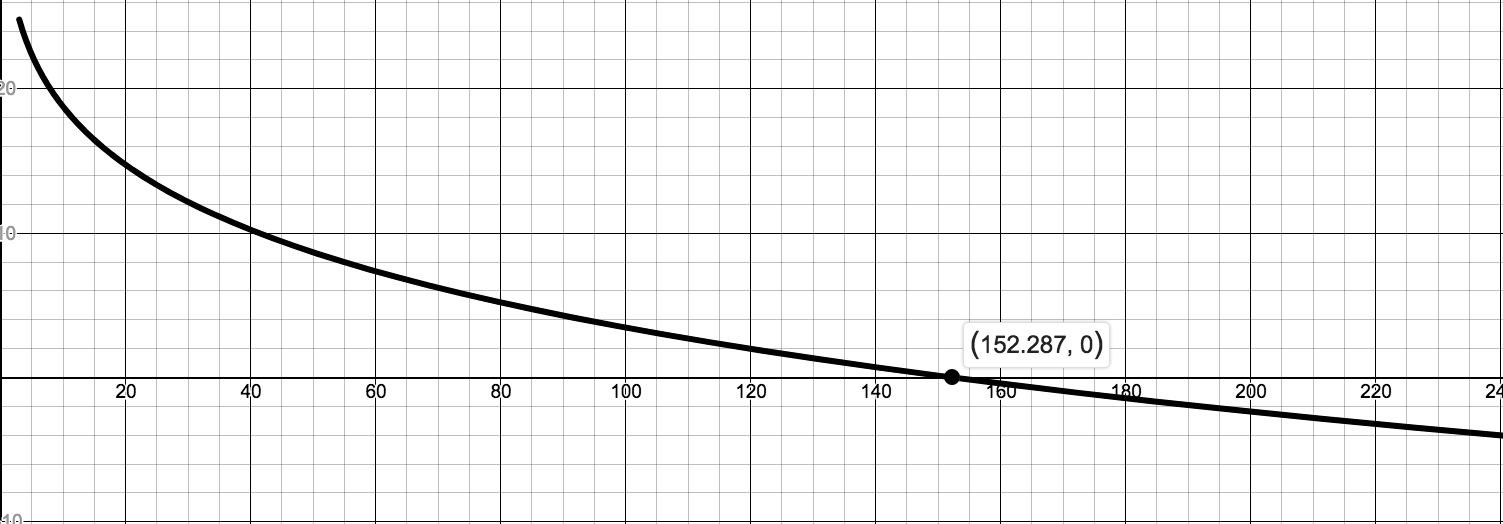
\includegraphics[height=1.75in]{./PowerFunctionsGraphics/WINDCHILL.jpg}}

\end{enumerate}



\item \begin{enumerate}

\item  $y = \frac{1}{3}x^{\frac{3}{2}} - x^{\frac{1}{2}} + \frac{2}{3}$.  The point $\left(0,\frac{2}{3}\right)$ is when Fritzy's path crosses Chewbacca's path - in other words, where Fritzy catches Chewbacca.

\begin{center} 

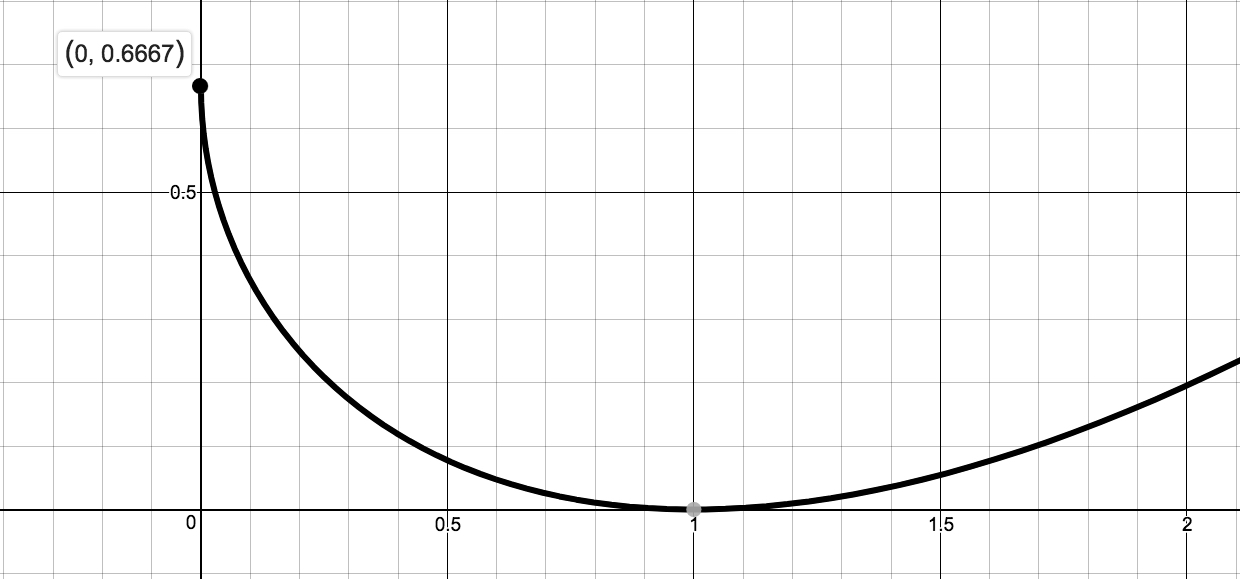
\includegraphics[height=2in]{./PowerFunctionsGraphics/PURSUIT01.jpg}

 $y = \frac{1}{3}x^{\frac{3}{2}} - x^{\frac{1}{2}} + \frac{2}{3}$

\end{center}

\item $y = \frac{1}{6}x^3+\frac{1}{2}x^{-1} - \frac{2}{3}$.  We find as $x \rightarrow 0^{+}$, $y \rightarrow \infty$ which means, in this case, Fritzy's pursuit never ends;  he never catches Chewbacca. This makes sense since Chewbacca has a head start and is running faster than Fritzy.

\begin{center} 

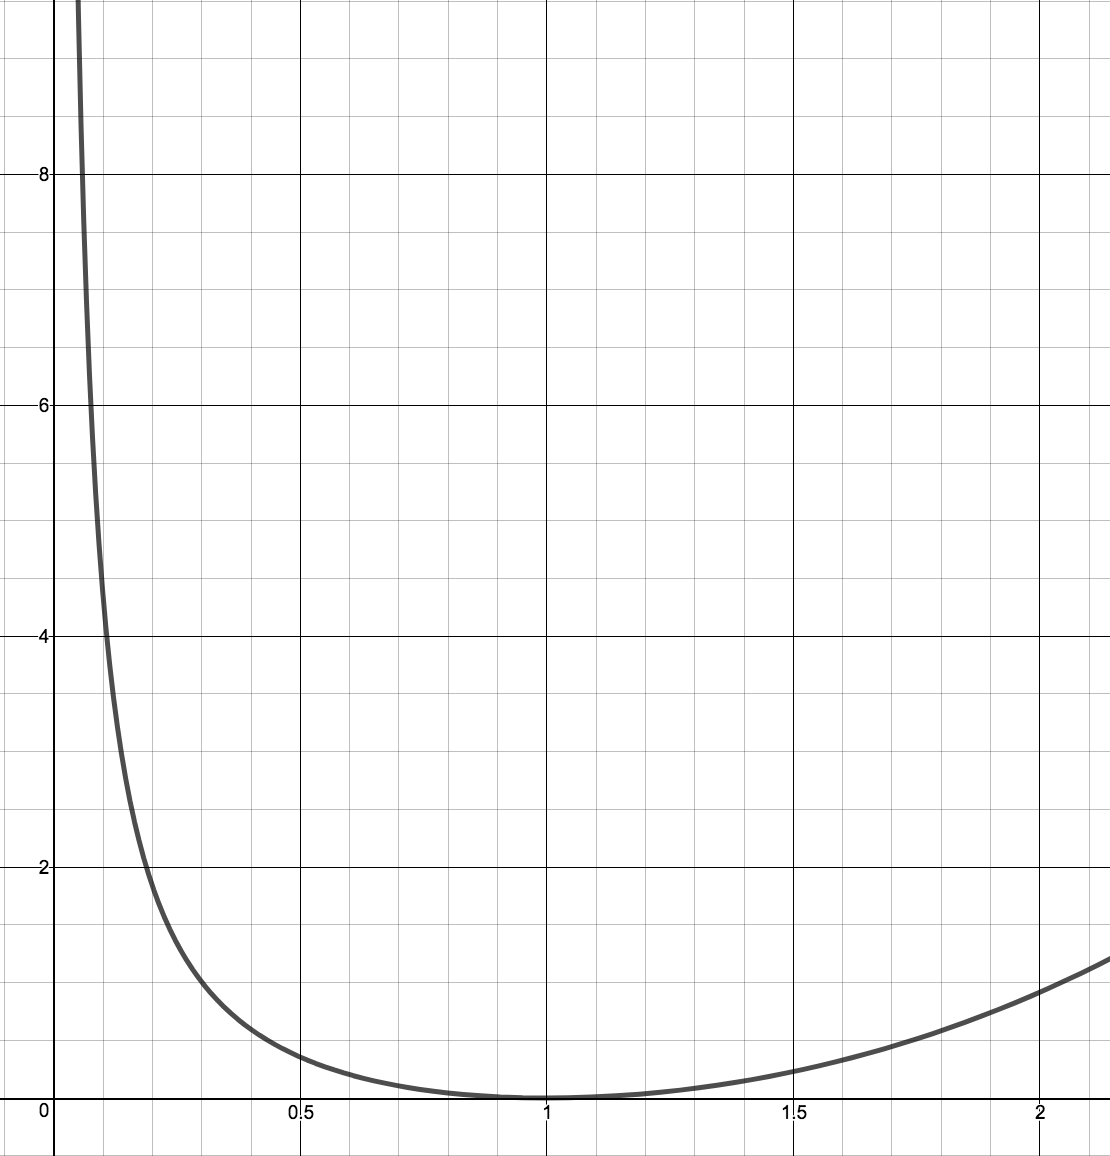
\includegraphics[height=2in]{./PowerFunctionsGraphics/PURSUIT02.jpg}

 $y = \frac{1}{6}x^3+\frac{1}{2}x^{-1} - \frac{2}{3}$

\end{center}


\end{enumerate}






\setcounter{HW}{\value{enumi}}
\end{enumerate}




\closegraphsfile

\end{document}


\newpage

\section{Equations and Inequalities involving Power Functions}

\documentclass{ximera}

\begin{document}
	\author{Stitz-Zeager}
	\xmtitle{TITLE}


\mfpicnumber{1}

\opengraphsfile{PowerEqIneq}

\setcounter{footnote}{0}

\label{PowerEqIneq}

In this section, we set about solving equations and inequalities involving power functions.  Our first example demonstrates the usual sorts of strategies to employ when solving equations.

\begin{example} \label{powerequationex}  Solve the following equations analytically and verify your answers using a graphing utility.


\begin{multicols}{2}
\begin{enumerate}

\item \label{first} $(7-x)^{\frac{3}{2}} = 8$ 
\item \label{second} $(2t-1)^{\frac{2}{3}} -4 = 0$

\setcounter{HW}{\value{enumi}}
\end{enumerate}
\end{multicols}

\begin{multicols}{2}
\begin{enumerate}
\setcounter{enumi}{\value{HW}}

\item $(x+3)^{0.5} = 2(7-x)^{0.5}+1$ 
\item $2t^{\frac{2}{3}} + 5t^{\frac{1}{3}} = 3$

\setcounter{HW}{\value{enumi}}
\end{enumerate}
\end{multicols}


\begin{multicols}{2}
\begin{enumerate}
\setcounter{enumi}{\value{HW}}

\item $2(3x-1)^{-0.5}  = 3x (3x-1)^{-1.5}$ 
\item $6(9-t^2)^{\frac{1}{3}} = 4t^2 (9-t^2)^{-\frac{2}{3}}$

\setcounter{HW}{\value{enumi}}
\end{enumerate}
\end{multicols}

{\bf Solution.}

\begin{enumerate}

\item  One way to proceed to solve  $(7-x)^{\frac{3}{2}} = 8$ is to use Definition \ref{rationalexponentdefna} to rewrite $(7-x)^{\frac{3}{2}}$ as either $(\sqrt{7-x})^3$ or $\sqrt{(7-x)^3}$.  We opt for the former since, thinking ahead,  $8$ is a perfect cube: 

\[ \begin{array}{rclr}

(7-x)^{\frac{3}{2}} & = & 8 & \\

(\sqrt{7-x})^3 & = & 8 & \text{rewrite using Definition \ref{rationalexponentdefna}} \\

\sqrt[3]{(\sqrt{7-x})^3} & = & \sqrt[3]{8} & \text{extract cube roots}  \\

\sqrt{7-x} & = & 2 & \text{$\sqrt[3]{u^3}= u$} \\ \end{array} \]

From $\sqrt{7-x} =  2$, we square both sides and obtain $7-x = 4$, so $x = 3$.  We verify our answer analytically by substituting $x=3$ into the original equation and it checks.

Geometrically, we are looking for where the graph of $f(x) = (7-x)^{\frac{3}{2}}$ intersects the graph of $g(x) = 8$.  While we could sketch both curves by hand and gauge the reasonableness of the result,\footnote{consider this an exercise!} we are instructed to use a graphing utility.  Below on the left and see the intersection point of both graphs is $(3,8)$, thereby checking our solution $x = 3$.

\item  Proceeding similarly to the above, to solve $(2t-1)^{\frac{2}{3}} -4 = 0$, we rewrite $(2t-1)^{\frac{2}{3}}$ as $(\sqrt[3]{2t-1})^2$ and solve:

\[ \begin{array}{rclr}
(2t-1)^{\frac{2}{3}} -4  & = & 0 & \\

(\sqrt[3]{2t-1})^2 - 4 & = & 0 & \text{rewrite using Definition \ref{rationalexponentdefna}} \\
(\sqrt[3]{2t-1})^2 & = & 4 & \text{isolate the variable term} \\

\sqrt{(\sqrt[3]{2t-1})^2 } & = & \sqrt{4} & \text{extract square roots} \\

|\sqrt[3]{2t-1}| & = & 2 & \text{$\sqrt{u^2} = |u|$} \\

\sqrt[3]{2t-1} & = & \pm 2 & \text{ for $c>0$, $|u| = c$ is equivalent to $u = \pm c$.} \end{array} \]

From $\sqrt[3]{2t-1}  = 2$ we cube both sides and obtain $2t-1 = 8$, so $t = \frac{9}{2} = 4.5$.  Similarly, from $\sqrt[3]{2t-1}  = -2$, we cube both sides and obtain $2t-1 = -8$, so $t = -\frac{7}{2} = -3.5$.  Both of these solutions check in the given equation.

In this case we are looking for where the graph of $f(t) = (2t-1)^{\frac{2}{3}} -4$ intersects the graph of $g(t) = 0$ - i.e., the $t$-intercepts of the graph of $g$.  We find these are $(-3.5,0)$ and $(4.5,0)$, as predicted.

\begin{center}

\begin{tabular}{cc}

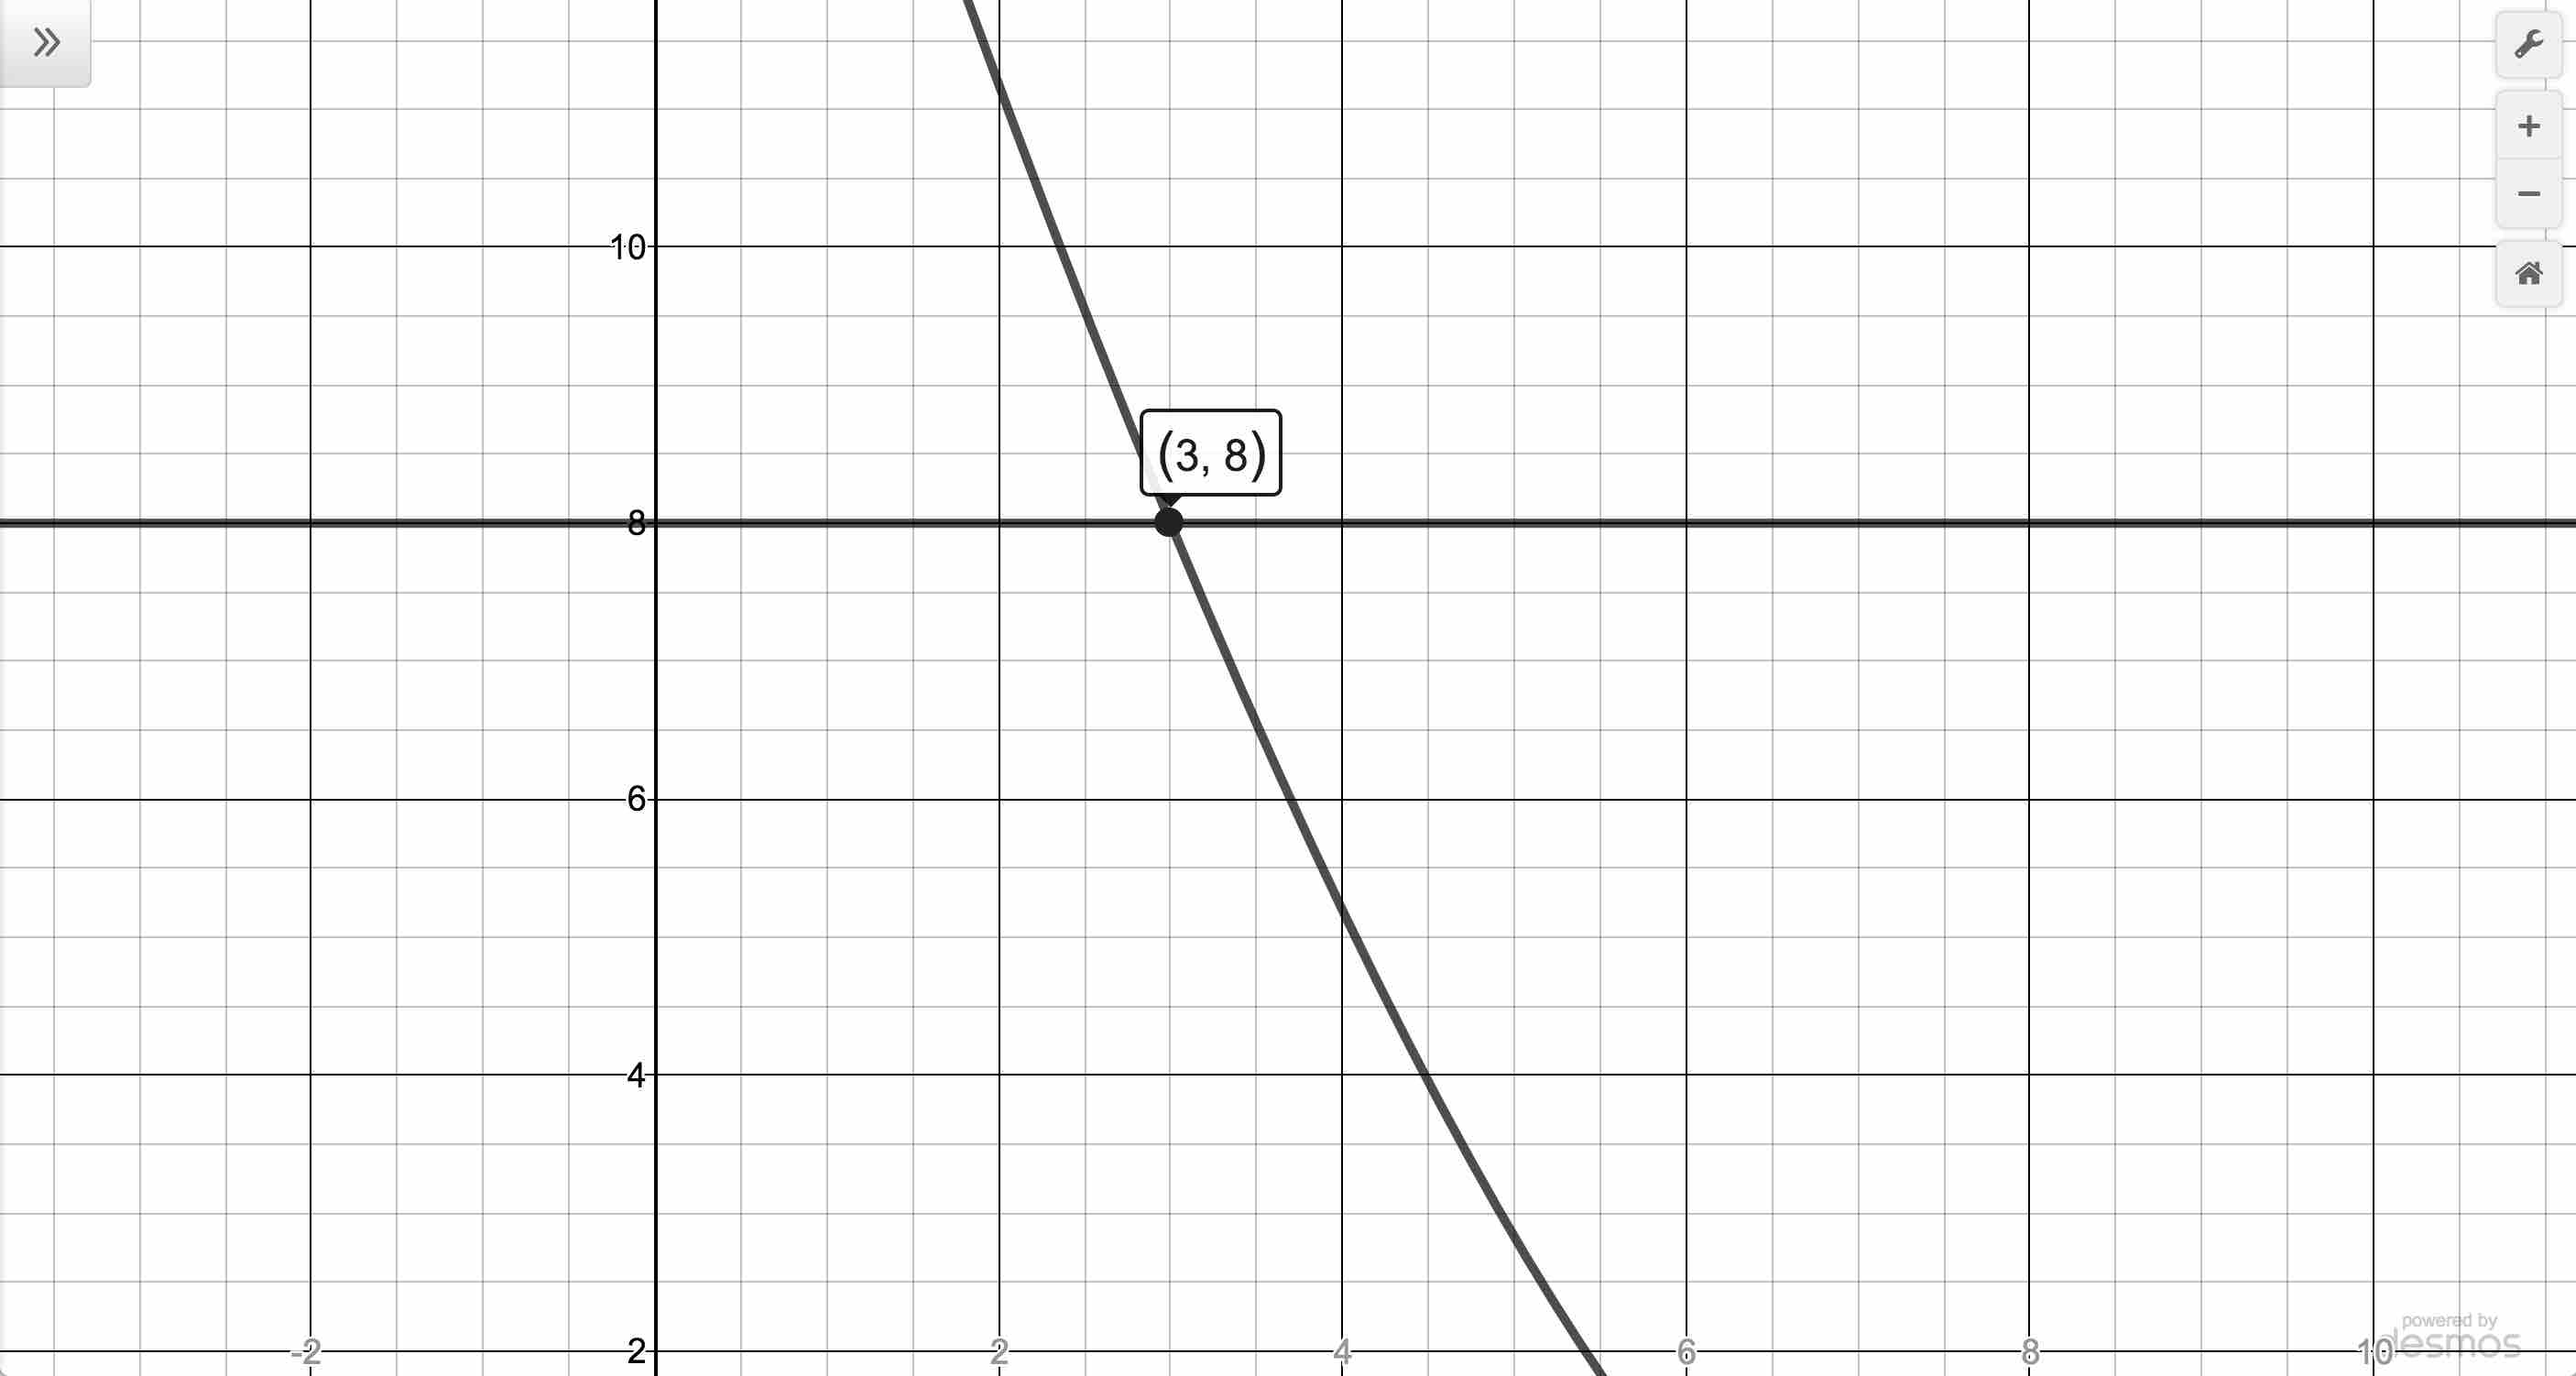
\includegraphics[width=3in]{./PowerEqIneqGraphics/PowerEqEx01.jpg} & 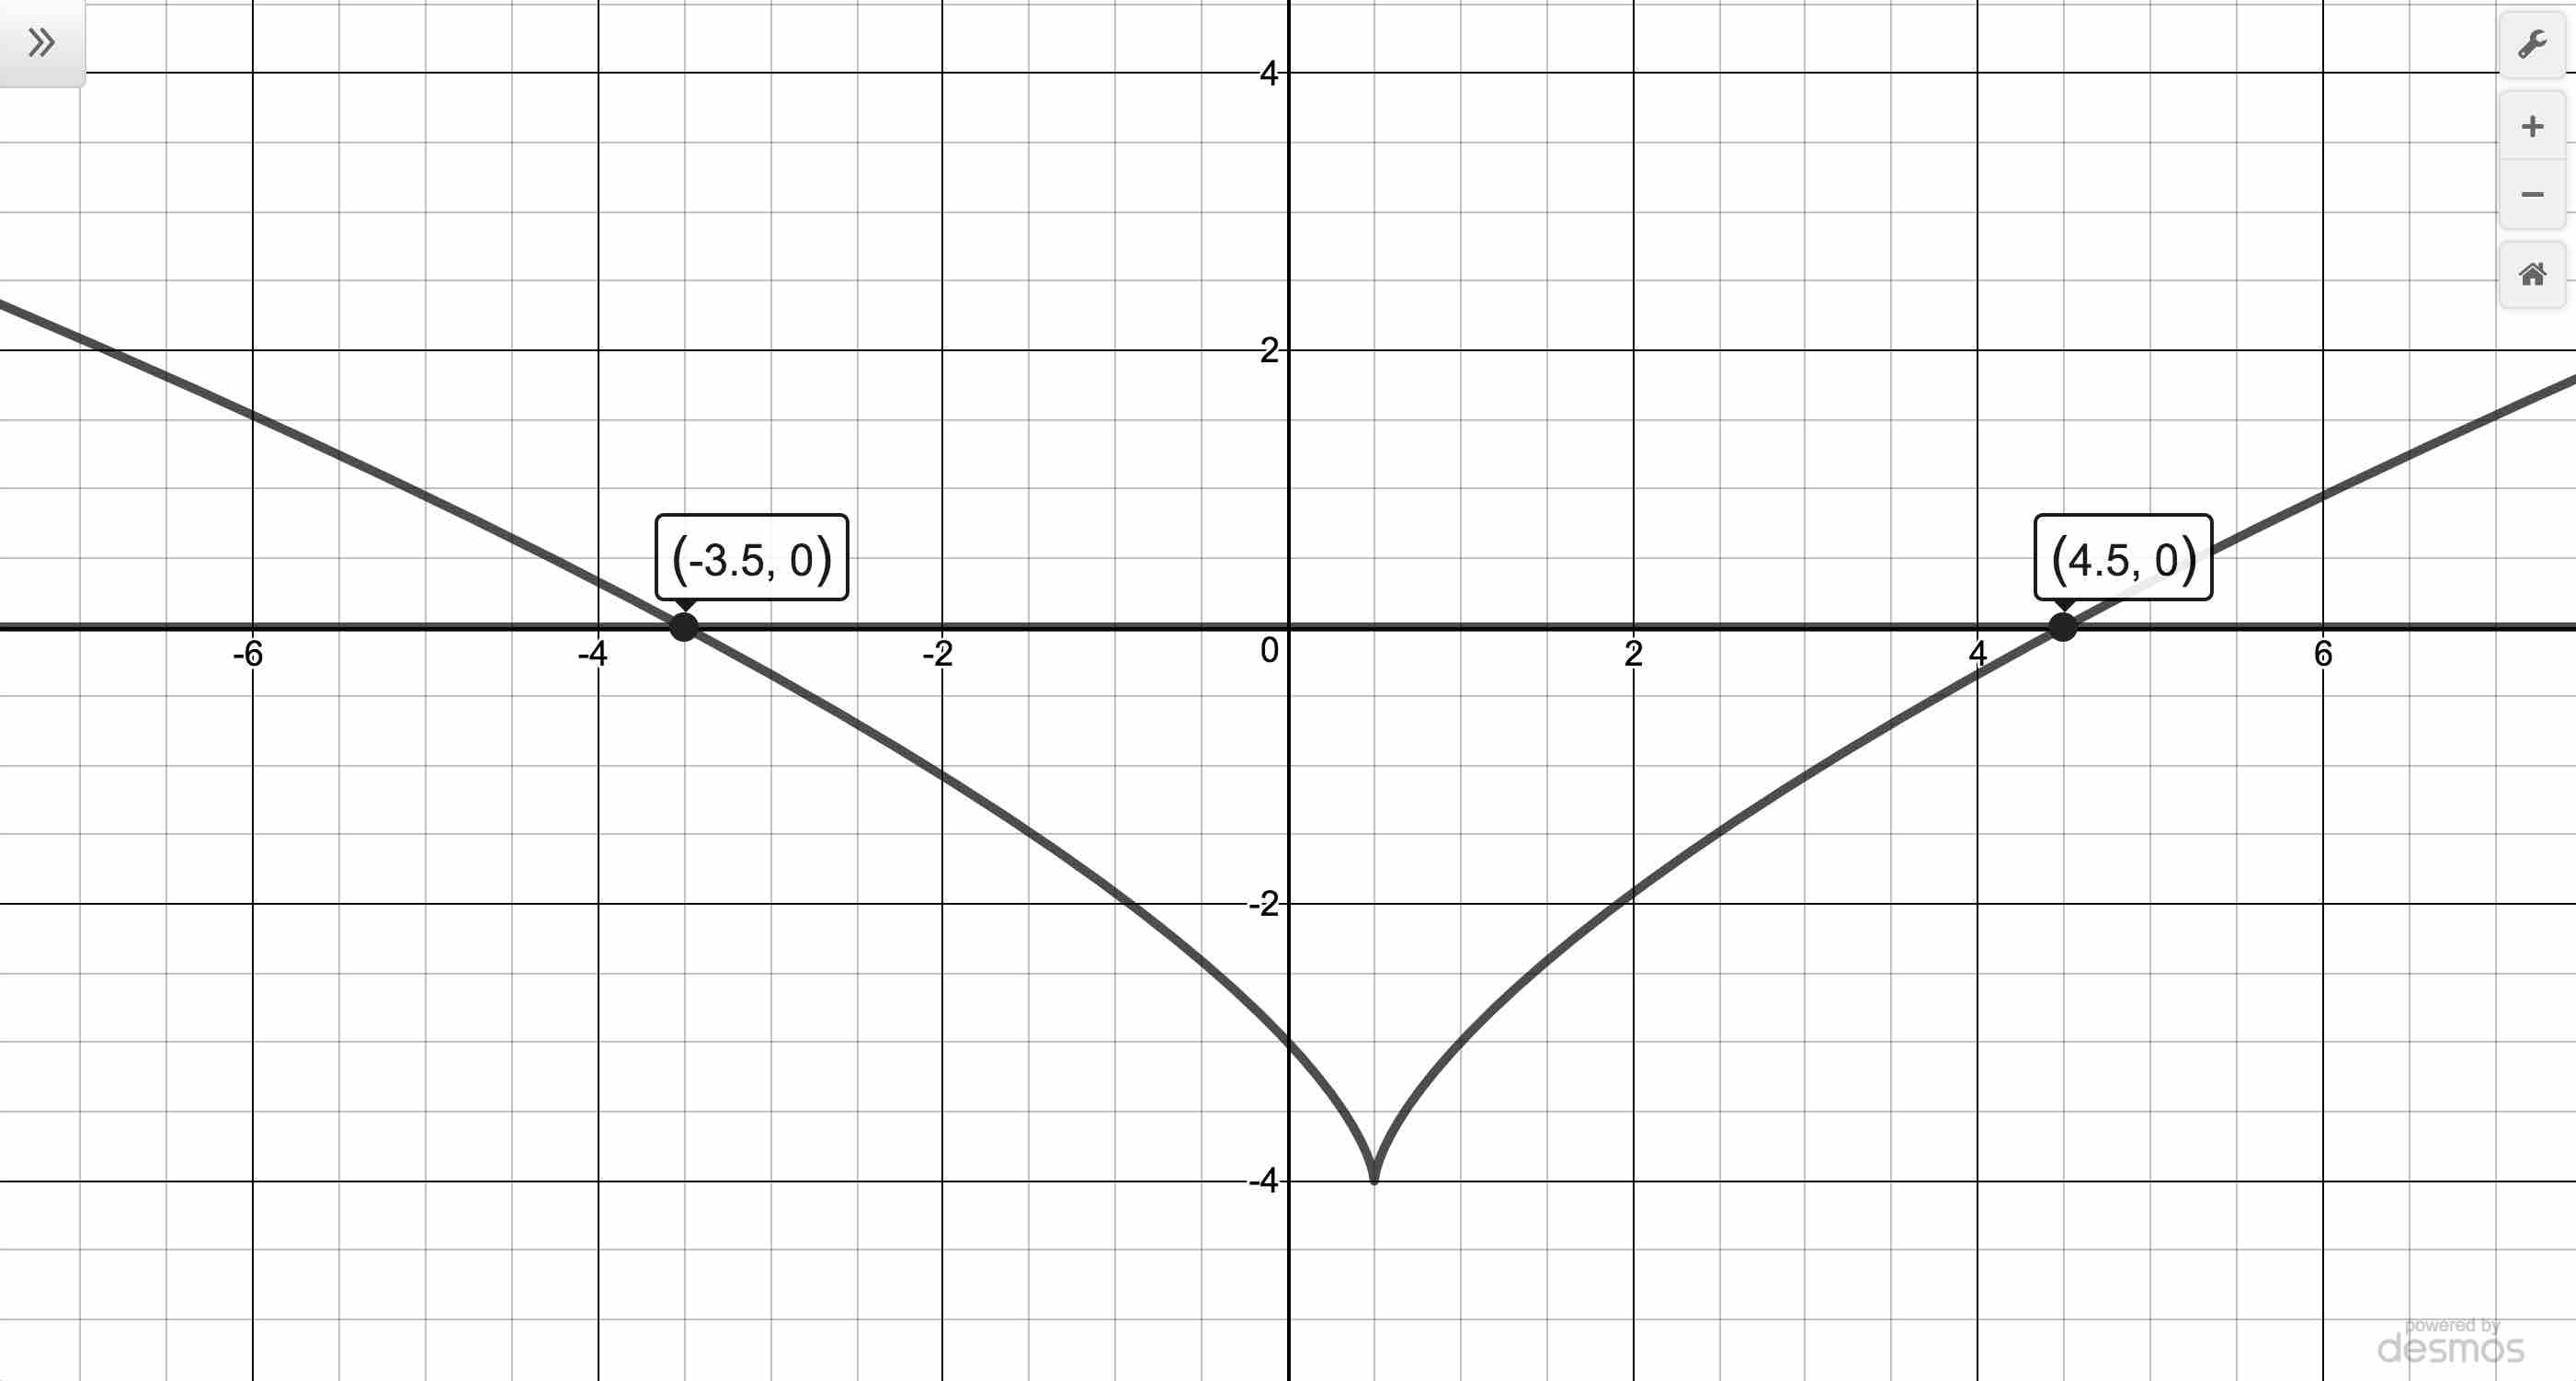
\includegraphics[width=3in]{./PowerEqIneqGraphics/PowerEqEx02.jpg} \\

Checking $(7-x)^{\frac{3}{2}} = 8$  & Checking  $(2t-1)^{\frac{2}{3}} -4 = 0$ \\

\end{tabular}

\end{center} 

\item Since $0.5 = \frac{1}{2}$, we may rewrite $(x+3)^{0.5} = 2(7-x)^{0.5}+1$ as  $(x+3)^{\frac{1}{2}} = 2(7-x)^{\frac{1}{2}}+1$.  Using Definition \ref{rationalexponentdefna}, we then have $\sqrt{x+3} = 2\sqrt{7-x} + 1$.  Since one of the square roots is already isolated, we can rid ourselves of it by squaring both sides.

\[ \begin{array}{rclr}

\sqrt{x+3} & = & 2\sqrt{7-x} + 1 & \\

 (\sqrt{x+3})^2 & = & (2\sqrt{7-x} + 1)^2 & \text{square both sides} \\
 
 x+3 & = & (2 \sqrt{7-x})^2 + 2 (2 \sqrt{7-x})(1) + 1 & \text{$(\sqrt{u})^2 = u$ and $(a+b)^2 = a^2 + 2ab +b^2$} \\

 
 x+3 & = & 4(7-x) + 4\sqrt{7-x} + 1 &  \text{$(ab)^2 = a^2b^2$ and, again, $(\sqrt{u})^2 = u$} \\
 
 x+3 & = & 28-4x+4\sqrt{7-x} + 1 & \\
 
 5x-26 & = & 4\sqrt{7-x} & \text{isolate $\sqrt{7-x}$} \\ \end{array} \]
 
We square both sides \textit{again} and get $(5x-26)^2 = (4\sqrt{7-x})^2$ which reduces to $25x^2-260x+676 = 16(7-x)$. At last, we have a quadratic equation which we can solve by setting to zero and factoring.  We get  $25x^2-244x+564 = 0$, so $(x-6)(25x-94) = 0$ so $x = 6$ or $x = \frac{94}{25} = 3.76$.  When we go to check these answers, we find $x=6$ does check, but $x = 3.76$ does not. Hence, $x=3.76$ is an `extraneous' solution.\footnote{We invite the reader to see at which point in our machinations $x=3.76$ \textit{does} check.  Knowing a solution is extraneous is one thing;  understanding \textit{how} it came about is another.}

We graph both $f(x) = \sqrt{x+3}$ and $g(x) = 2\sqrt{7-x} + 1$ below (once again, we could graph these by hand!) and confirm there is only one intersection point, $(6,3)$.

\item  While we \textit{could} approach solving  $2t^{\frac{2}{3}} + 5t^{\frac{1}{3}} = 3$ as the previous example, we would encounter cubing binomials\footnote{that is, expanding things like $(a+b)^3$.} which we would prefer to avoid.  Instead, we take a step back and notice there are three terms here with the exponent on one term, $t^{\frac{2}{3}}$ exactly twice the exponent on another term, $t^{\frac{1}{3}}$.  We have ourselves a `quadratic in disguise.'\footnote{See Section \ref{AppQuadEqus} or, more recently, Example \ref{polyquadinform} in Section \ref{RealZeros}.} To help us see the forest for the trees, we let $u = t^{\frac{1}{3}}$ so that $u^2 = t^{\frac{2}{3}}$. (Note that since root here, $3$, is odd, we can use the properties of exponents stated in Theorem \ref{exponentprops}.)  Hence, in terms of $u$, the equation   $2t^{\frac{2}{3}} + 5t^{\frac{1}{3}} = 3$ becomes the quadratic $2u^2 + 5u = 3$, or $2u^2 + 5u - 3 = 0$.  Factoring gives $(2u-1)(u+3) = 0$ so $u = t^{\frac{1}{3}} = \frac{1}{2}$ or $u = t^{\frac{1}{3}} = -3$.  Since $t^{\frac{1}{3}} = \sqrt[3]{t}$, we solve both equations by cubing both sides to get $t = \frac{1}{8} = 0.125$ and $t = -27$.  Both of these solutions check in our original equation.  Looking at the graphs of $f(t) = 2t^{\frac{2}{3}} + 5t^{\frac{1}{3}}$ and $g(t) = 3$, we find two intersection points, $(-27,3)$ and $(0.125,3)$, as required.

\begin{center}

\begin{tabular}{cc}

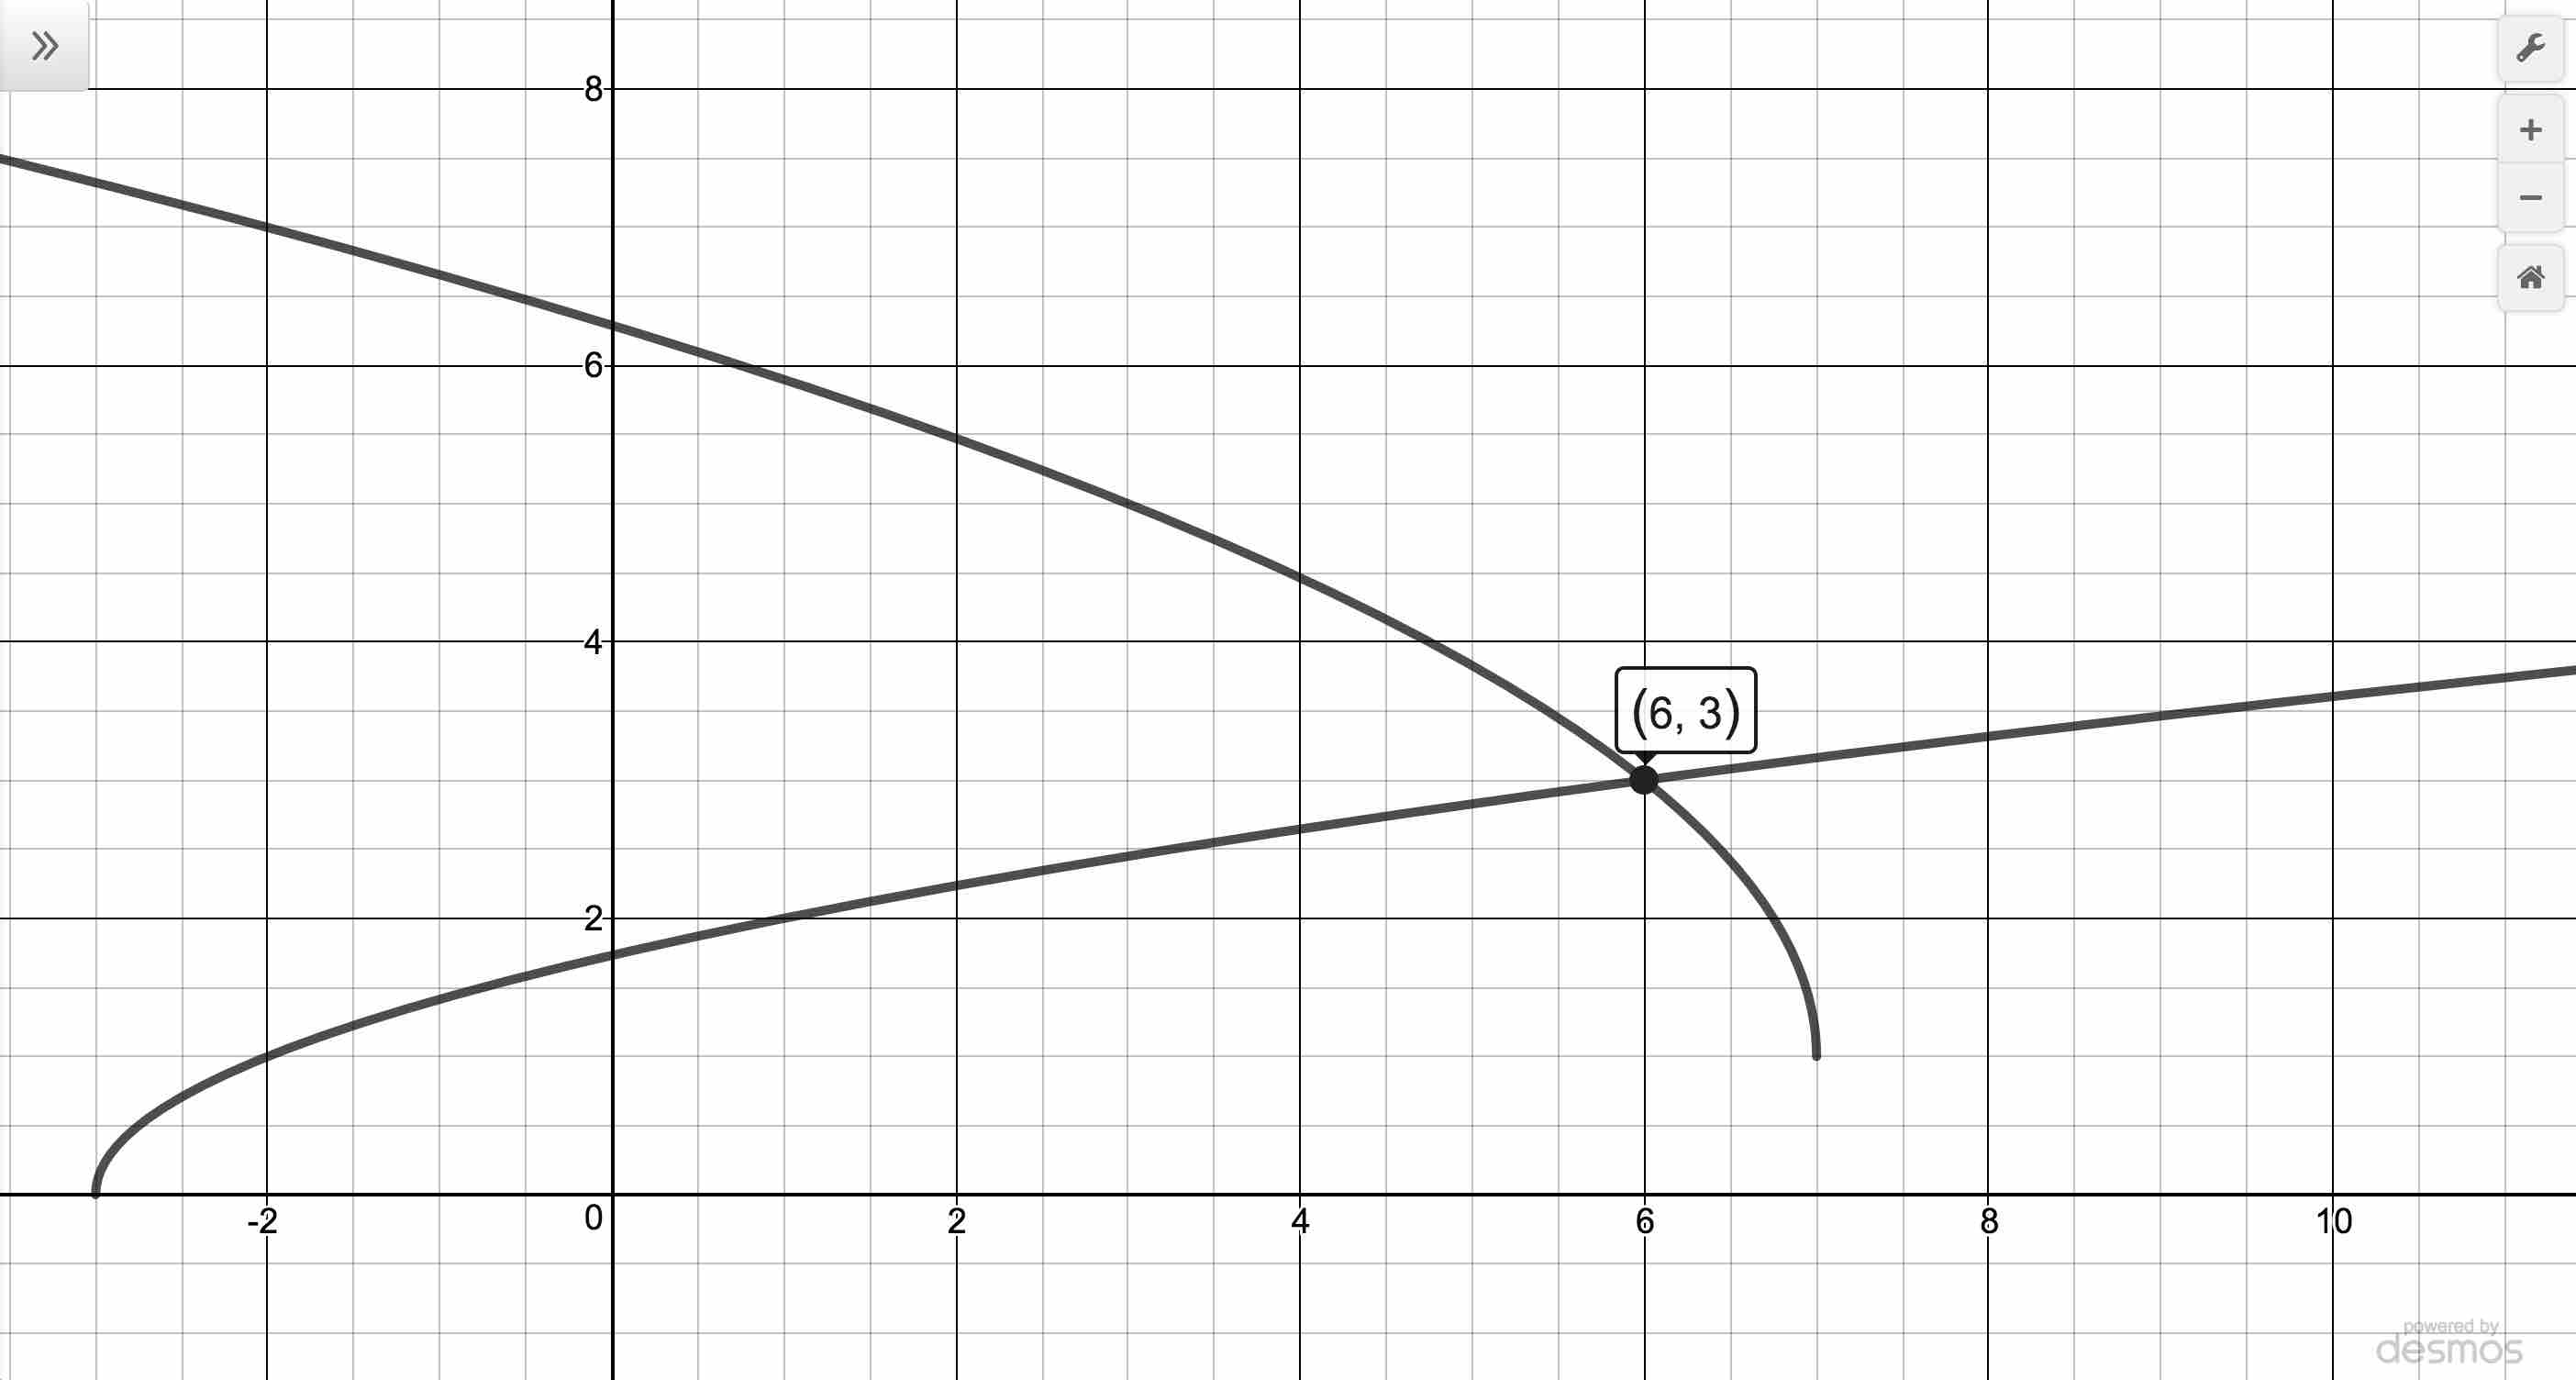
\includegraphics[width=3in]{./PowerEqIneqGraphics/PowerEqEx03.jpg} & 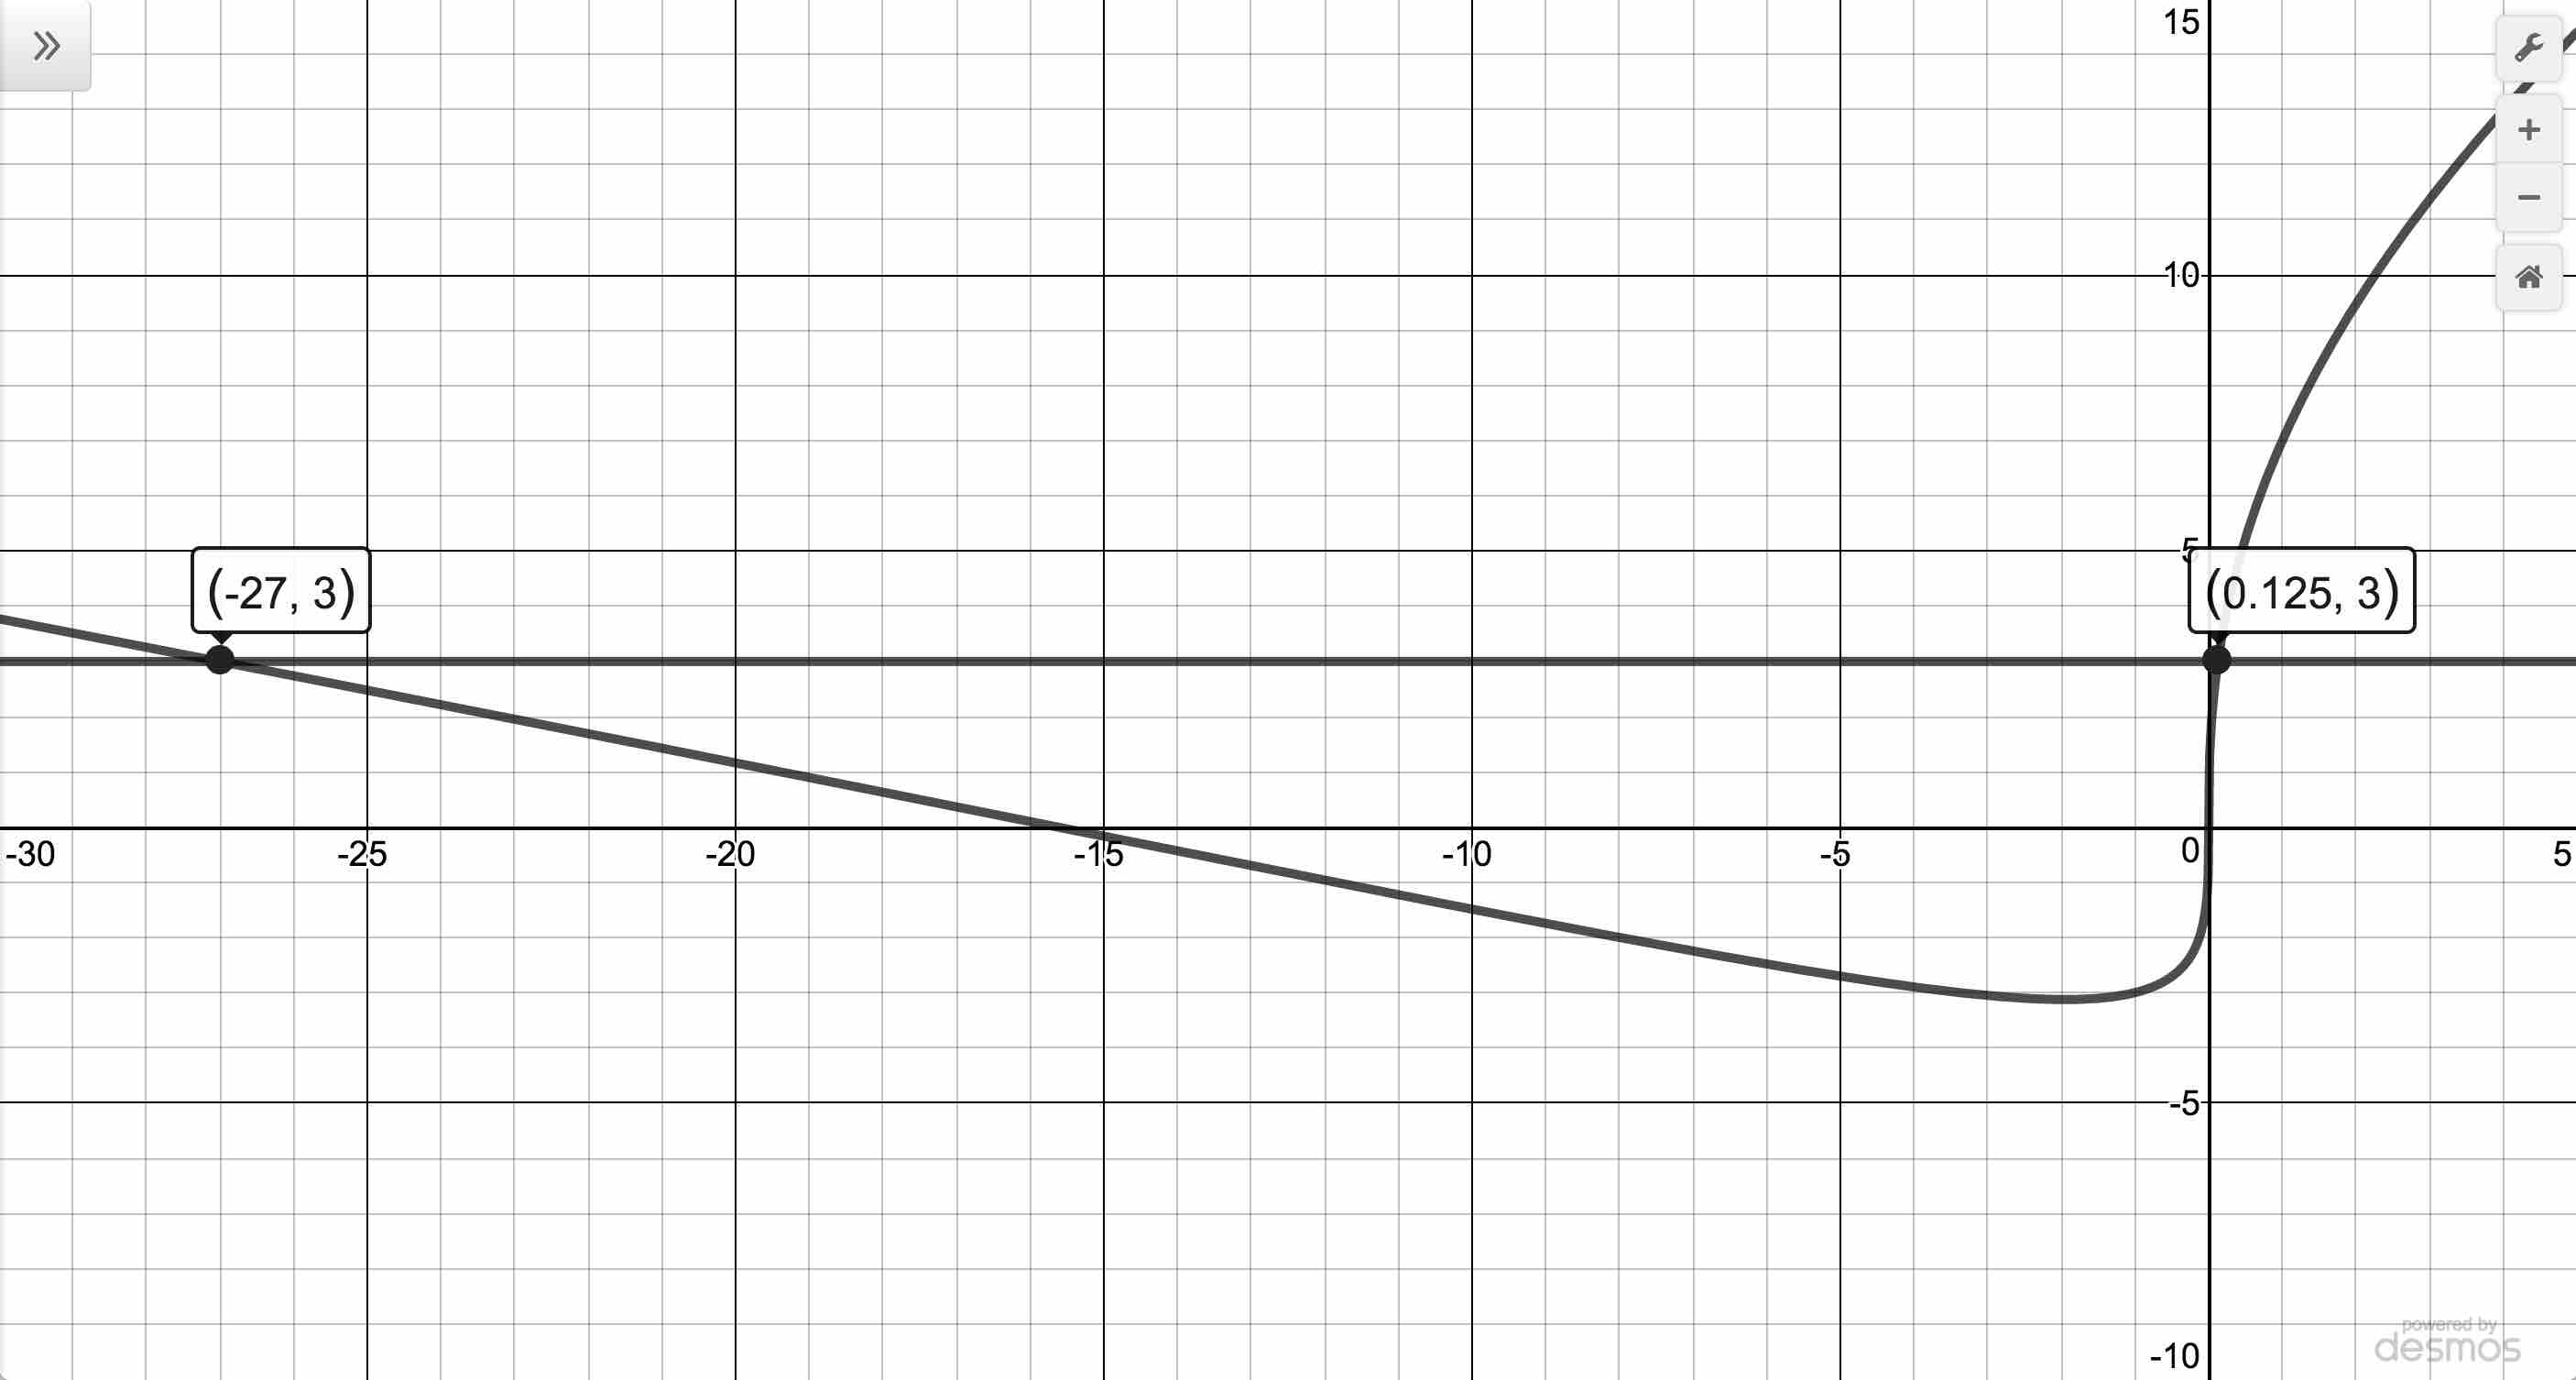
\includegraphics[width=3in]{./PowerEqIneqGraphics/PowerEqEx04.jpg} \\

Checking $(x+3)^{0.5} = 2(7-x)^{0.5}+1$ & Checking  $2t^{\frac{2}{3}} + 5t^{\frac{1}{3}} = 3$ \\

\end{tabular}

\end{center} 


\item Next we are to solve $2(3x-1)^{-0.5}  = 3x (3x-1)^{-1.5}$ which, when written without negative exponents is: $\frac{2}{(3x-1)^{0.5}} = \frac{3x}{(3x-1)^{1.5}}$.  Since the rational exponents here are $0.5 = \frac{1}{2}$ and $1.5 = \frac{3}{2}$, both involve an \textit{even} indexed root (the square root in this case!) which means $3x-1 \geq 0$.  Moreover, since the $3x-1$ resides in the \textit{denominator} $3x - 1 \neq 0$ so our equation is really valid only for values of $x$ where $3x-1>0$ or $x > \frac{1}{3}$.  Hence, we clear denominators and can apply Theorem \ref{exponentprops}:

\[ \begin{array}{rclr}

\dfrac{2}{(3x-1)^{0.5}} & = & \dfrac{3x}{(3x-1)^{1.5}} & \\

\left[ \dfrac{2}{(3x-1)^{0.5}} \right] \cdot (3x-1)^{1.5} & = & \left[  \dfrac{3x}{(3x-1)^{1.5}} \right ] \cdot (3x-1)^{1.5} & \\

2 \cdot \dfrac{(3x-1)^{1.5}}{(3x-1)^{0.5}} & = & 3x & \\

2 (3x-1)^{1.5-0.5} & = & 3x & \text{Theorem \ref{exponentprops} applies since $3x-1 > 0$.} \\

2 (3x-1)^{1} & = & 3x & \\  \end{array} \]

We get $6x-2 = 3x$, or $x = \frac{2}{3}$.  Since $x = \frac{2}{3} > \frac{1}{3}$, we keep it and, sure enough, it  checks in our original equation. Graphically we see $f(x)=2(3x-1)^{-0.5}$ intersects $g(x) = 3x (3x-1)^{-1.5}$ at the point $(0.6667, 2)$ which is the graphing utility's way of representing $\left(\frac{2}{3}, 2\right)$.

\item  Our last equation to solve is $6(9-t^2)^{\frac{1}{3}} = 4t^2 (9-t^2)^{-\frac{2}{3}}$, which, when rewritten without negative exponents is: $6(9-t^2)^{\frac{1}{3}} = \frac{4t^2}{(9-t^2)^{\frac{2}{3}}}$  .   Again, the root here ($3$) is odd, so we can use the exponent properties listed in Theorem \ref{exponentprops}.   We begin by clearing denominators: 


\[ \begin{array}{rclr}

6(9-t^2)^{\frac{1}{3}} & = & \frac{4t^2}{(9-t^2)^{\frac{2}{3}}} & \\

6(9-t^2)^{\frac{1}{3}} \cdot (9-t^2)^{\frac{2}{3}} & = & \left[   \frac{4t^2}{(9-t^2)^{\frac{2}{3}}}  \right ] \cdot (9-t^2)^{\frac{2}{3}} & \\

6(9-t^2)^{\frac{1}{3} + \frac{2}{3}}& = & 4t^2 &  \text{Theorem \ref{exponentprops} applies since the root here $3$ is odd.} \\

6(9-t^2)^{1} & = & 4t^2 &\\   \end{array} \]

We get $54 - 6t^2 = 4t^2$ or $10t^2 = 54$.  As fraction $t^2 = \frac{54}{10} = \frac{27}{5}$ so $t = \pm \sqrt{\frac{27}{5}} = \pm 3 \sqrt{15}{5}$.  While not the easiest to check analytically, both of these solutions do work in the original equation.  Graphing $f(t) = 6(9-t^2)^{\frac{1}{3}} $ and $g(t) =  4t^2 (9-t^2)^{-\frac{2}{3}}$ below, we see the graphs intersect when $t \approx \pm 2.324$ which are decimal approximations of our exact answers.

\begin{center}

\begin{tabular}{cc}

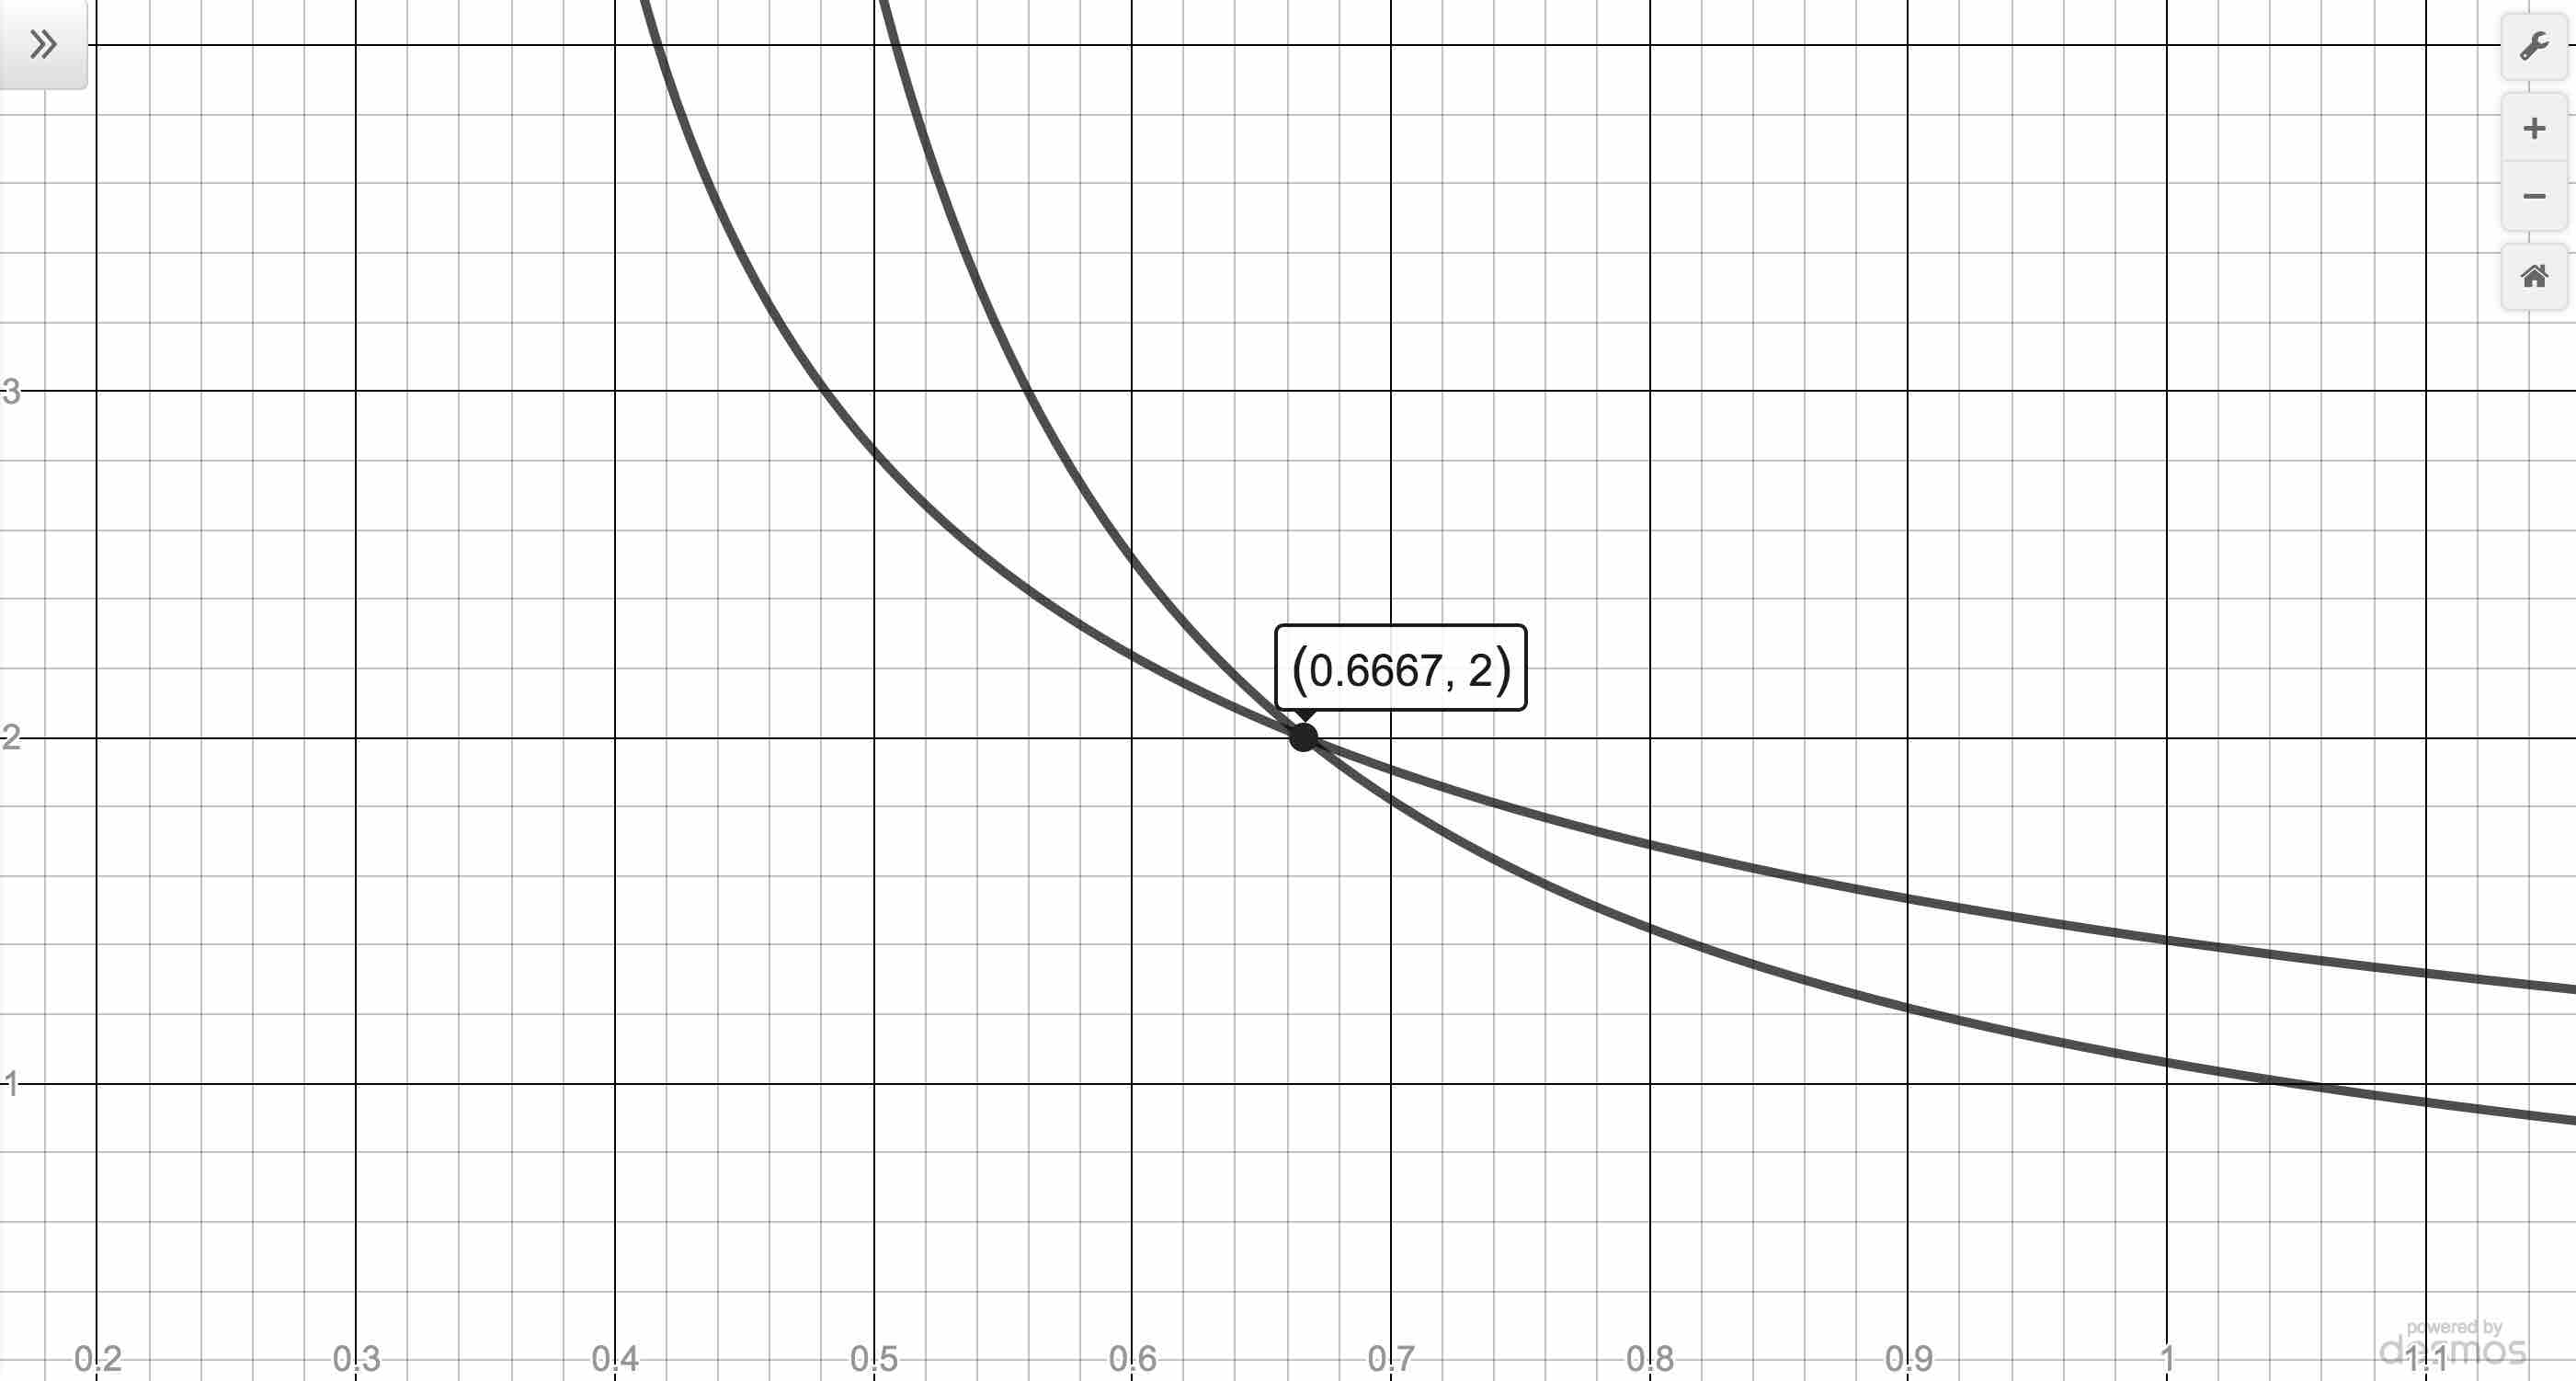
\includegraphics[width=3in]{./PowerEqIneqGraphics/PowerEqEx05.jpg} & 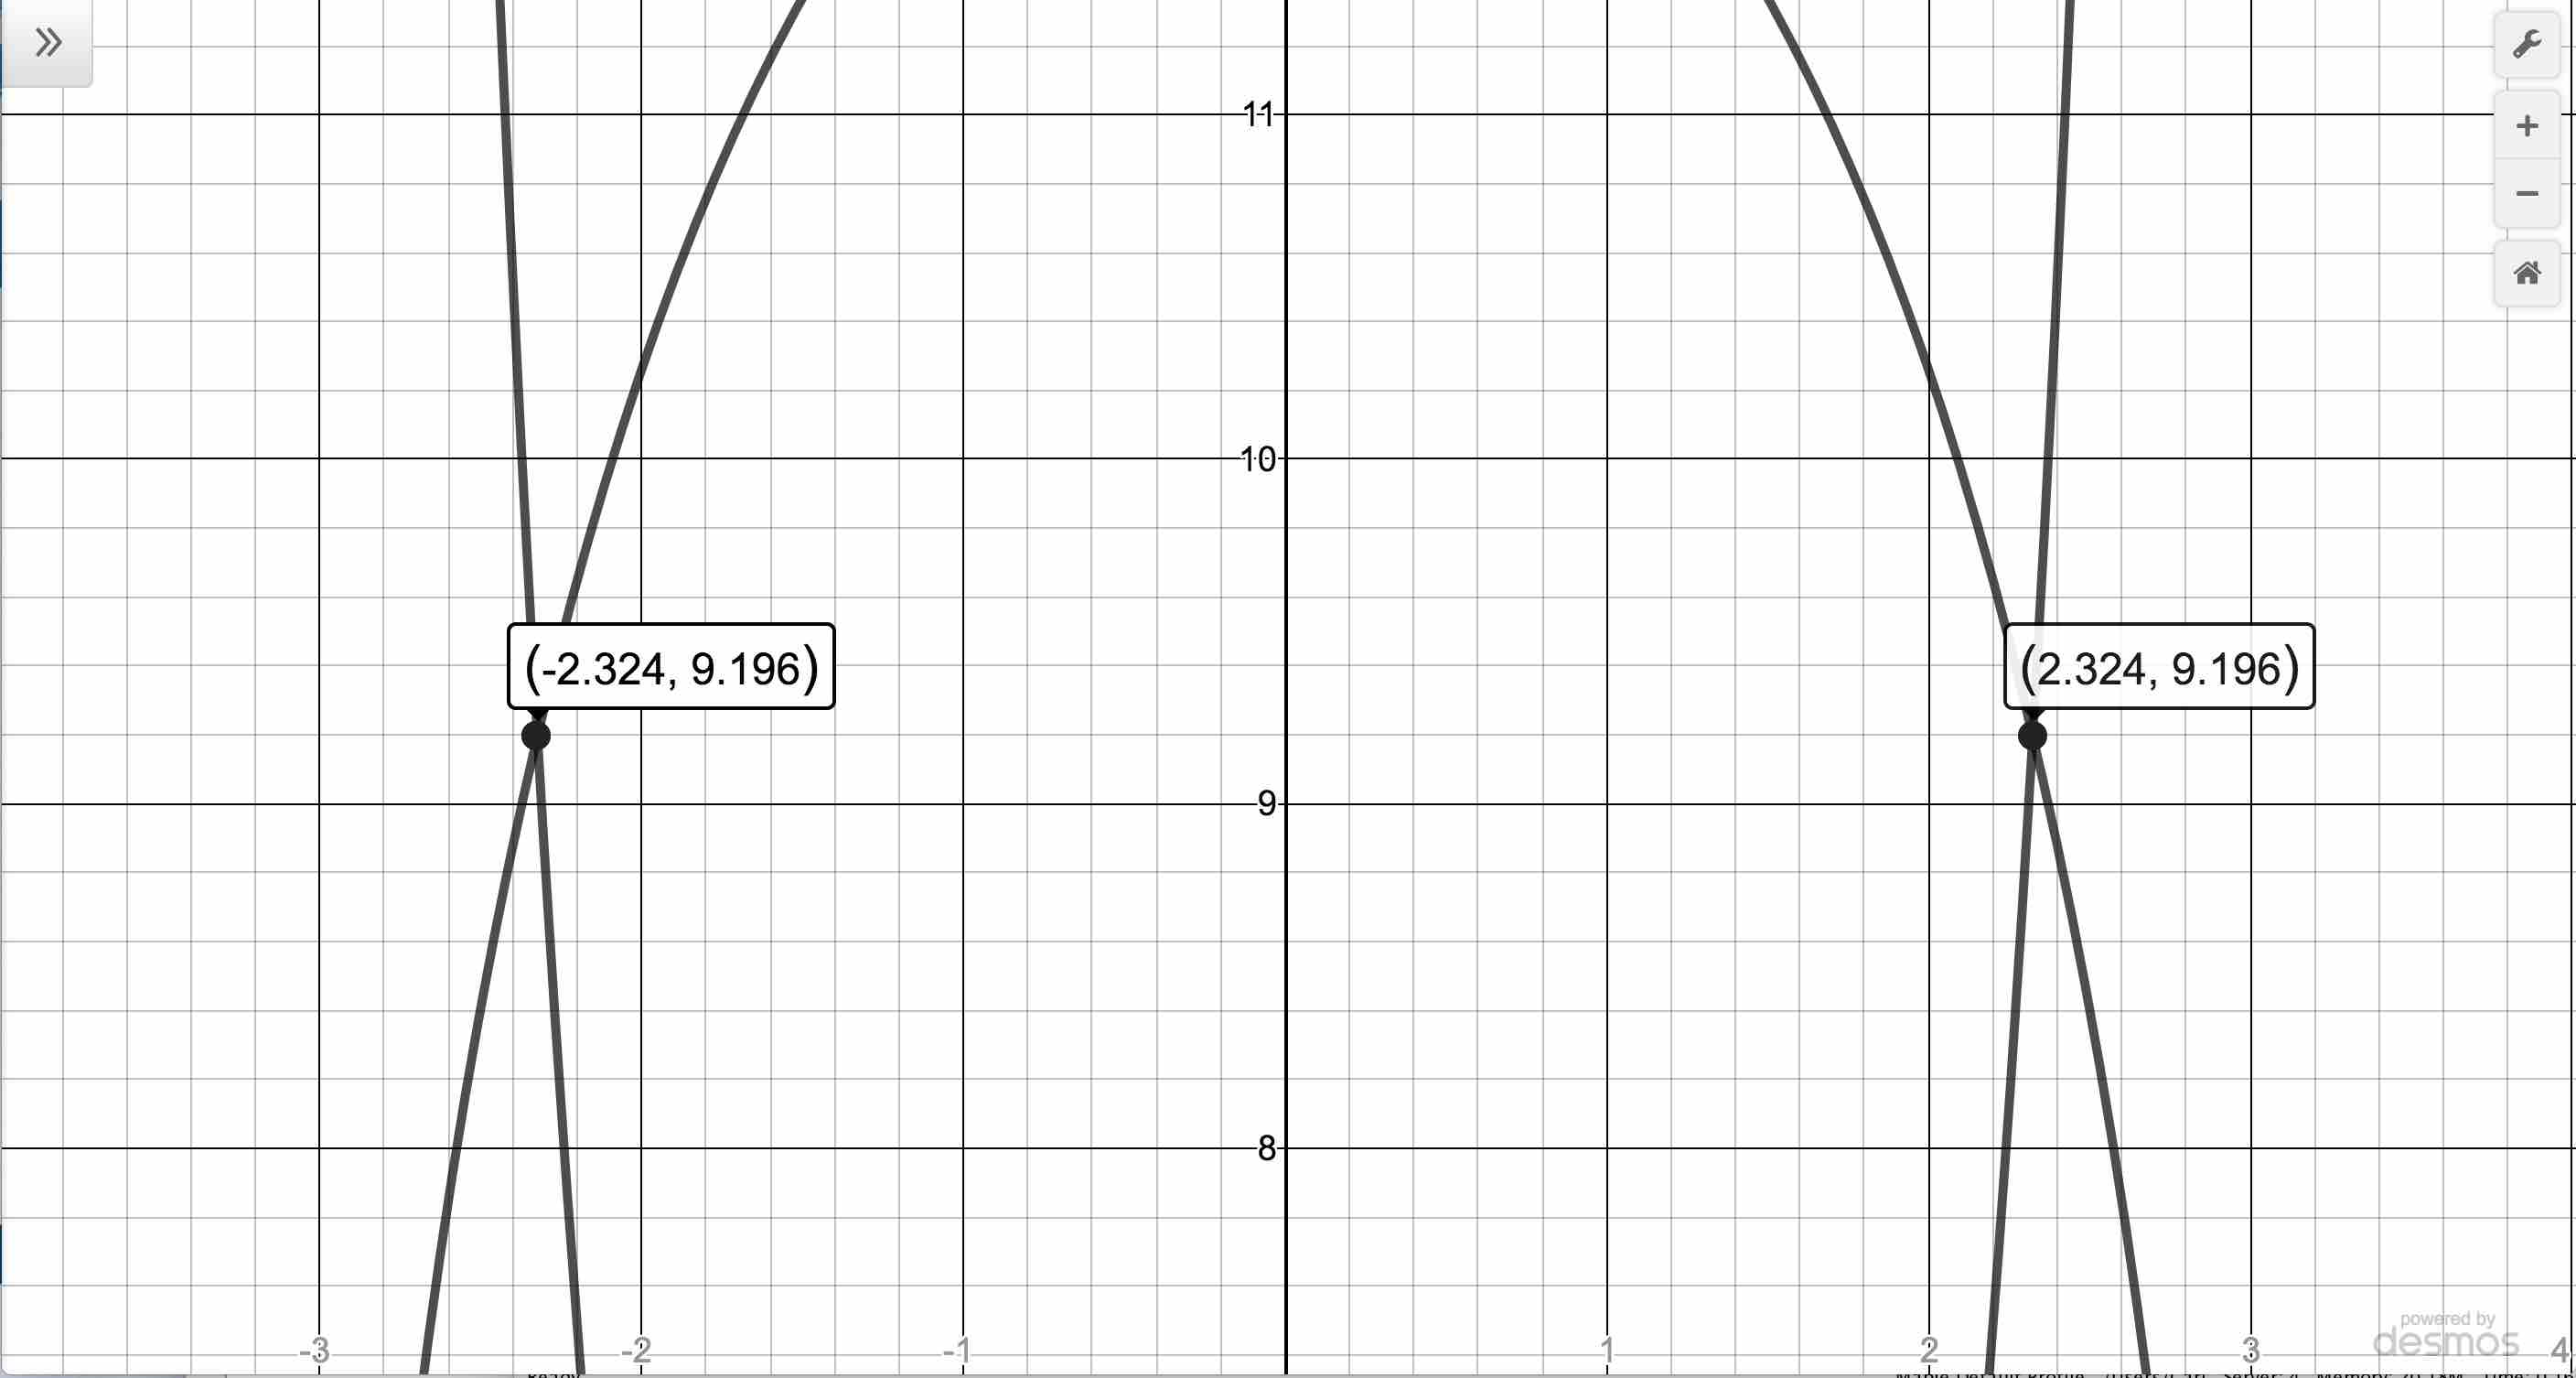
\includegraphics[width=3in]{./PowerEqIneqGraphics/PowerEqEx06.jpg} \\

Checking $2(3x-1)^{-0.5}  = 3x (3x-1)^{-1.5}$  & Checking  $6(9-t^2)^{\frac{1}{3}} = 4t^2 (9-x^2)^{\frac{2}{3}}$ \\

\end{tabular}

\end{center} 

\end{enumerate}

\qed

\end{example}

Note that Example \ref{powerequationex}, there are several ways to correctly solve each equation, and we endeavored to demonstrate a variety of methods.  For example, for number \ref{first}, instead of converting $(7-x)^{\frac{3}{2}}$ to a radical equation, we could use Theorem \ref{exponentprops}.  Since the root here ($2$) is even, we know $7-x \geq 0$ or $x \leq 7$.  Hence we may apply exponent properties: 

\[ \begin{array}{rclr}  

(7-x)^{\frac{3}{2}} & = & 8 & \\

 \left[(7-x)^{\frac{3}{2}}\right]^{\frac{2}{3}} & = & 8^{\frac{2}{3}} & \text{raise both sides to the $\frac{2}{3}$ power} \\
 
 (7-x)^{\frac{3}{2} \cdot \frac{2}{3}} & = & 4 & \text{Theorem \ref{exponentprops}} \\
 
(7-x)^{1} & = & 4 \\ \end{array} \]

from which we get $x = 3$.  If we try this same approach to solve number \ref{second}, however, we encounter difficulty.  From $(2t-1)^{\frac{2}{3}} -4 = 0$, we get $(2t-1)^{\frac{2}{3}}  =4$.  

\[ \begin{array}{rclr}  

(2t-1)^{\frac{2}{3}} & = & 4 & \\

 \left[(2t-1)^{\frac{2}{3}}  \right]^{\frac{3}{2}} & = & 4^{\frac{3}{2}}& \text{raise both sides to the $\frac{3}{2}$ power} \\ \end{array} \]
 
 Since the root here ($3$) is odd, we have no restriction on $2t-1$ but the exponent $\frac{3}{2}$ has an even denominator.  Hence, Theorem \ref{exponentprops} \textit{does not apply}.  That is, \[\left[(2t-1)^{\frac{2}{3}}  \right]^{\frac{3}{2}} \neq (2t-1)^{\frac{2}{3} \cdot \frac{3}{2}} = (2t-1)^{1} = (2t-1).\]
 Note that if we weren't careful, we'd have $2t-1 = 4^{\frac{3}{2}} = 8$ which gives $t= \frac{9}{2} = 4.5$ only.   We'd have missed the solution $t = -3.5$.  Truth be told, you \textit{can} simplify $\left[(2t-1)^{\frac{2}{3}}  \right]^{\frac{3}{2}} $ - just not using Theorem \ref{exponentprops}.  We leave it as an exercise to show  $\left[(2t-1)^{\frac{2}{3}}  \right]^{\frac{3}{2}} = |2t-1|$ and, more generally, $\left(x^{\frac{2}{3}}\right)^{\frac{3}{2}} = |x|$.
 
 Our next example is an application of the  \href{https://en.wikipedia.org/wiki/Cobb-Douglas_production_function}{\underline{Cobb Douglas}} production model of an economy.  The Cobb-Douglas model states that the yearly total dollar value of the production output in an economy is a function of \textit{two} variables:   labor (the total number of hours worked in a year) and capital (the total dollar value of the physical goods required for manufacturing.) The equation relating the production output level $P$, labor $L$ and capital $K$ takes the form $P = a L^{b} K^{1-b}$ where $0 < b < 1$; that is, the production level varies jointly with some power of the labor and capital.  

\begin{example} \label{CobbDouglasEx}  In their original paper \textit{A Theory of Production}\footnote{available \href{http://bit.ly/2dxlstt}{\underline{here}}.} Cobb and Douglas modeled the output of the US Economy (using 1899 as a baseline) using the formula $P = 1.01 L^{0.75} K^{0.25}$ where $P$, $L$, and $K$ were percentages of the 1899 figures for total production, labor, and capital, respectively.

\begin{enumerate}

\item  For 1910, the recorded labor and capital figures for the US Economy are $144 \%$ and $208 \%$ of the 1899 figures, respectively.  Find $P$ using these figures and interpret your answer.

\item  The recorded production value figure for 1920 is $231 \%$ of the 1899 figure.  Use this to write $K$ as a function of $L$, $K = f(L)$.  Find and interpret $f(193)$.

\item  Graph $K = f(L)$ and interpret the behavior as $L \rightarrow 0^{+}$ and $L \rightarrow \infty$.


\end{enumerate}

{\bf Solution.}

\begin{enumerate}

\item  In this case, $P = 1.01 L^{0.75} K^{0.25} = 1.01 (144)^{0.75} (208)^{0.25} \approx 159$ which means the dollar value of the total US Production in 1920 was approximately $159 \%$ of what it was in 1899.\footnote{This answer is remarkably accurate. Note:  all the dollar values here are recorded in `1880' dollars, per the source article. }  


\item We are given $P = 231 = 1.01L^{0.75} K^{0.25}$, so to write $K$ as a function of $L$, we need to solve this equation for $K$.  Since $L$ and $K$ are positive by definition, we can employ properties of exponents:

\[ \begin{array}{rclr}

231 & = & 1.01 L^{0.75} K^{0.25} & \\

\dfrac{231}{1.01 L^{0.75}} & = &  \dfrac{1.01 L^{0.75} K^{0.25}}{1.01 L^{0.75}} & \text{$L>0$, hence $L^{0.75} \neq 0$.}\\

K^{0.25} & = & 228.\overline{7128}L^{-0.75} & \text{rewrite} \\

\left(K^{0.25}\right)^{\frac{1}{0.25}} & = & \left(228.\overline{7128}L^{-0.75}\right)^{\frac{1}{0.25}} & \\

K^{\frac{0.25}{0.25}} & = & (228.\overline{7128})^{\frac{1}{0.25}} L^{-\frac{0.75}{0.25}} & \text{Theorem  \ref{exponentprops}} \\

K & = &  (228.\overline{7128})^{4} L^{-3} & \text{simplify} \\ \end{array} \]

Hence, $K = f(L) =  (228.\overline{7128})^{4} L^{-3}$ where $L>0$.  We find $f(193) =  (228.\overline{7128})^{4} (193)^{-3} \approx 381$ meaning that in order to maintain a production level of $231 \%$ of 1889 with a labor level at $193 \%$ of 1889, the required capital is $381 \%$ that of 1889.\footnote{The actual recorded figure is 407.}

\item The function $f(L)$ is a Laurent Monomial (see Section \ref{IntroRational}) with $n = 3$ and $a = (228.\overline{7128})^{4}$.  As such, as $L \rightarrow 0^{+}$, $f(L) \rightarrow \infty$.  This means that in order to maintain the given production level, as the available labor diminishes, the capital requirement become unbounded.  As $L \rightarrow \infty$, we have $f(L) \rightarrow 0$ meaning that as the available labor increases, the need for capital diminishes.  The graph of $f$ is called an `isoquant' - meaning `same quantity.'  In this context, the graph displays all combinations of labor and capital, $(L,K)$  which result in the \textit{same} production level, in this case, $231 \%$ of what was produced in 1889.

\begin{center}

\begin{mfpic}[25]{-1}{3}{-1}{3}
\axes
\scriptsize
\tlabel[cc](3, -0.5){$L$}
\tlabel[cc](-0.5, 3){$K$}
\tlabel[cc](2.5,1){$(1, (228.\overline{7128})^{4})$}
\normalsize
\penwd{1.25pt}
\arrow \reverse \arrow \function{0.7,2,0.1}{1/(x**3)}
\point[4pt]{(1,1)}
\tcaption{\scriptsize $K = f(L) =  (228.\overline{7128})^{4} L^{-3}$}
\end{mfpic}

\end{center}

\end{enumerate}

\qed

\end{example}

Next, we move on to solving inequalities with power functions.  As we've seen with other types of non-linear inequalities,\footnote{see Sections \ref{QuadraticFunctions}, \ref{RealZeros}, and \ref{RationalIneq}} an invaluable tool for us is the Sign Diagram.

\phantomsection
\label{algebraicsigndiagram}

%% \colorbox{ResultColor}{\bbm

\centerline{\textbf{Steps for Constructing a Sign Diagram for an Algebraic Function}} 

\medskip

\hspace{.17in} Suppose $f$ is an algebraic function. \index{sign diagram ! algebraic function}

\begin{enumerate}

\item  Place any values excluded from the domain of  $f$ on the number line with an `\textinterrobang' above them.

\item  Find the zeros of $f$ and place them on the number line with the number $0$ above them.

\item  Choose a test value in each of the intervals determined in steps 1 and 2.

\item  Determine and record the sign of $f(x)$ for each test value in step 3.

\end{enumerate}

%% \ebm}


As you may recall, since sign diagrams compare functions to $0$, the first step in solving inequalities using a sign diagram is to gather all the nonzero terms one one side of the inequality.  We demonstrate this technique in the following example.


\begin{example} \label{powerineqex} $~$

Solve the following inequalities.  Check your answers graphically with a calculator.

\begin{multicols}{2}
\begin{enumerate}

\item $2-\sqrt[4]{x+3} \geq 0$

\item $t^{2/3} < t^{4/3} - 6$


\setcounter{HW}{\value{enumi}}

\end{enumerate}
\end{multicols}

\begin{multicols}{2}
\begin{enumerate}

\setcounter{enumi}{\value{HW}}

\item  \label{third} $3 (2-x)^{\frac{1}{3}} \leq x (2-x)^{-\frac{2}{3}}$

\item \label{fourth} $(t-4)^{\frac{2}{3}} \geq -\dfrac{2t}{3(t-4)^{\frac{1}{3}}}$  


\end{enumerate}
\end{multicols}


{\bf Solution.}  

\begin{enumerate}

\item  To solve $2-\sqrt[4]{x+3} \geq 0$, it is tempting to rewrite this inequality as $2 \geq \sqrt[4]{x+3}$ and rid ourselves of the fourth root by raising both sides of this inequality to the fourth power.  While this technique works \textit{sometimes}, it doesn't work \textit{all} the time since raising both sides of an inequality to the fourth (more generally, to an even) power does not necessarily preserve inequalities .\footnote{For instance, $-2 \leq 1$ but $(-2)^{4} \geq (1)^2$.  We invite the reader to see what goes wrong if attempting to solve either of the following inequalities using this method: $-2 \geq \sqrt[4]{x+3}$, which has no solution, or  $-2 \leq \sqrt[4]{x+3}$, whose solution is $[-3,\infty)$.}  For that reason, we solve this inequality using a sign diagram since this technique will \textit{always} produce a correct solution.    

We already have all the nonzero terms on one side of the inequality, so we let $r(x) = 2-\sqrt[4]{x+3}$ and proceed to make a sign diagram.  Owing to the presence of the fourth root, we know $x+3 \geq 0$ or  $x \geq -3$.   Hence, we only concern ourselves with the portion of the number line representing $[3, \infty)$.  Next, we find the zeros of $r$ by solving $r(x) = 2-\sqrt[4]{x+3}=0$.  We get $\sqrt[4]{x+3} = 2$, so $x+3= 16$ and we get $x=13$.  We find this solution checks in our original equation,\footnote{Recall that raising both sides to an even power could produce extraneous solutions, so it is important we check here.}  and proceed to construct the sign diagram below on the left. Since we are looking for where $r(x) =  2-\sqrt[4]{x+3} \geq 0$, we are looking for the zeros of $r$ along with the intervals over which $r(x)$ is $(+)$.  We record our answer as $[-3, 13]$.  Below on the right is the graph of $y = 2-\sqrt[4]{x+3}$, and we can see that, indeed, the graph is above the $x$-axis ($y=0$) from $[-3, 13)$ and meets the $x$-axis at $x=13$, verifying our answer.

\begin{center}

\begin{tabular}{m{2in}m{2.5in}}

\begin{mfpic}[10]{0}{8}{-2}{2}

\arrow \polyline{(0,0), (8,0)}

\xmarks{0,4}

\tlabel[cc](0,-1){$-3 \hspace{7pt}$}

\tlabel[cc](2,1){$(+)$}

\tlabel[cc](4,-1){$13$}

\tlabel[cc](4,1){$0$}

\tlabel[cc](6,1){$(-)$}

\end{mfpic}

&

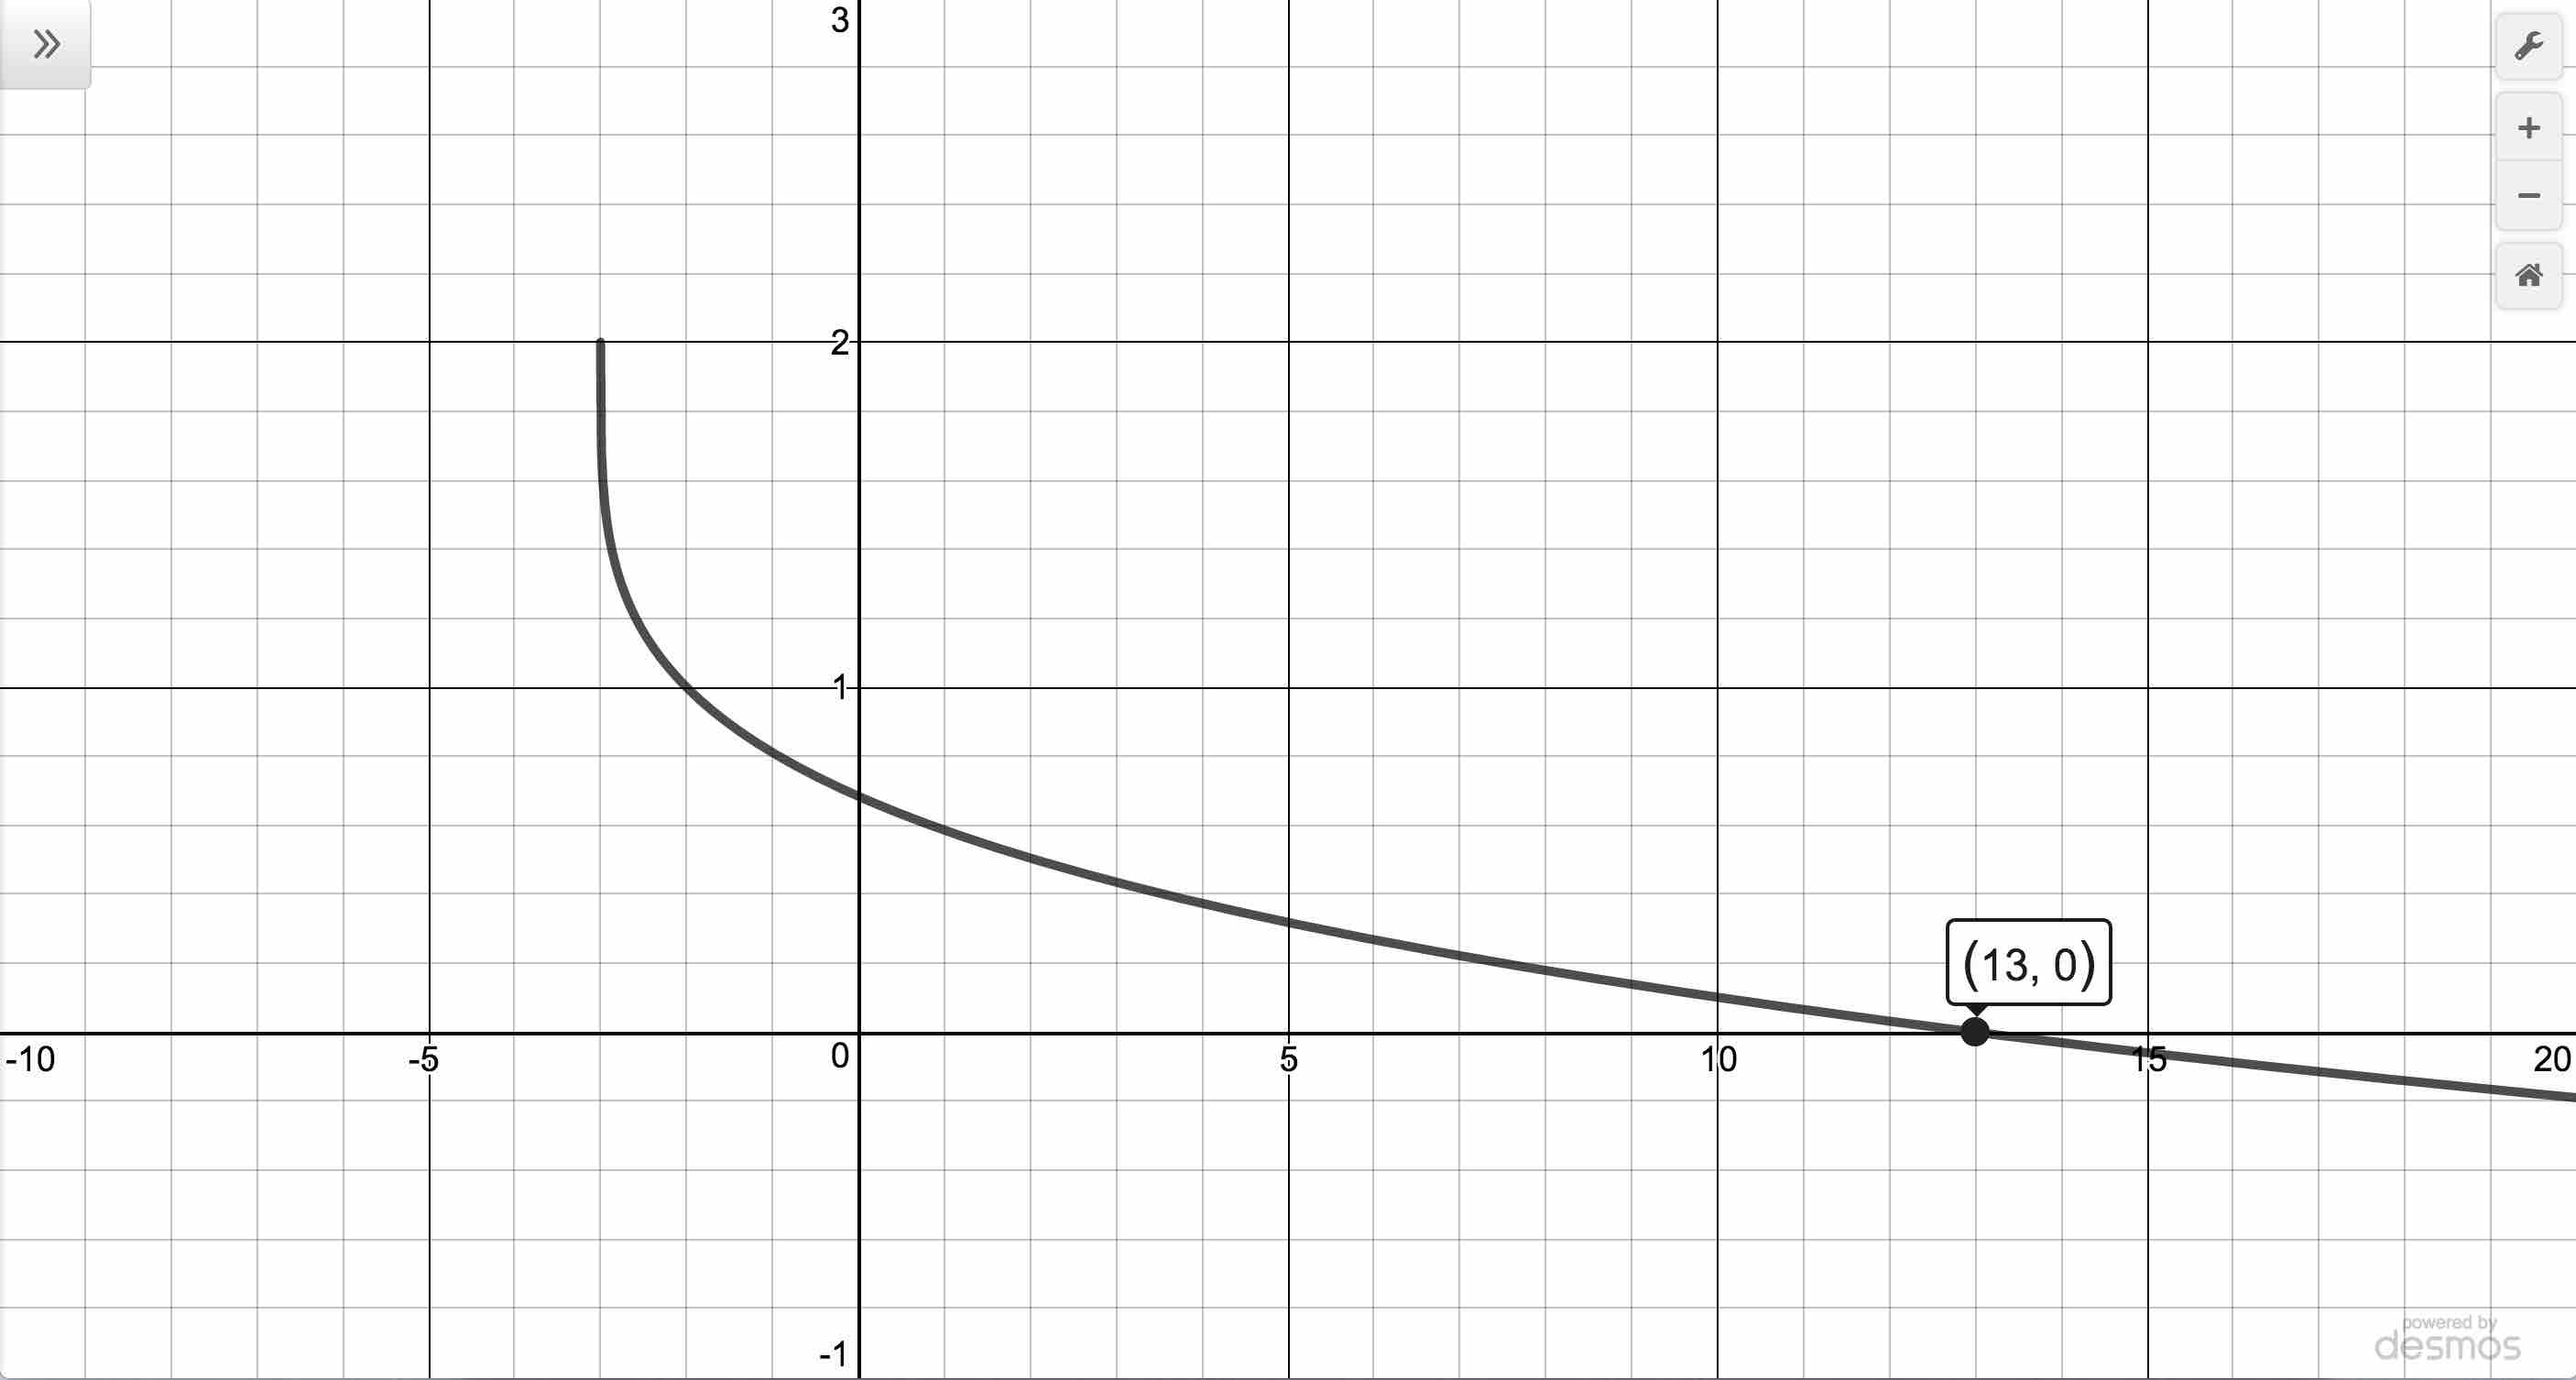
\includegraphics[width=3in]{./PowerEqIneqGraphics/PowerIneqEx01.jpg} \\ 

\end{tabular}

\end{center}

\item  To solve $t^{\frac{2}{3}} < t^{\frac{4}{3}} - 6$, we first rewrite as  $t^{\frac{4}{3}} -t^{\frac{2}{3}} - 6 > 0$.  We set $r(t) = t^{\frac{4}{3}} -t^{\frac{2}{3}} - 6$ and note that since the denominators in the exponents are $3$, they correspond to cube roots, which means the domain of $r$ is $(-\infty, \infty)$. To find the zeros for the sign diagram, we set $r(t) = 0$ and attempt to solve $t^{\frac{4}{3}} - t^{\frac{2}{3}} - 6 = 0$.   Since there are three terms, and the exponent on one of the variable terms, $t^{\frac{4}{3}}$, is exactly twice that of the other, $t^{\frac{2}{3}}$, we have ourselves a `quadratic in disguise.'   If we let $u = t^{\frac{2}{3}}$, then $u^2 = t^{\frac{4}{3}}$, so  in terms of $u$, we have $u^2 - u - 6 = 0$.  Solving  we get $u = -2$ or $u = 3$, hence  $t^{\frac{2}{3}} = -2$ or $t^{\frac{2}{3}} = 3$.  In root-power notation, these are $\sqrt[3]{t^2} = -2$ or $\sqrt[3]{t^2}= 3$.  Cubing both sides of these equations results in $t^2 = -8$, which admits no real solution, or $t^2 = 27$, which gives $t = \pm 3 \sqrt{3}$.  Using these zeros, we construct the sign diagram below on the left.  We find $r(t) = t^{\frac{4}{3}} -t^{\frac{2}{3}} - 6 > 0$  on $\left(-\infty, -3 \sqrt{3}\right)\cup \left(3 \sqrt{3}, \infty\right)$.  To check our answer graphically, we set $f(t) = t^{\frac{2}{3}}$ and $g(t) = t^{\frac{4}{3}}-6$.  The solution to  $t^{\frac{2}{3}} < t^{\frac{4}{3}} - 6$ corresponds to the inequality $f(t) < g(t)$, which means we are looking for the $t$ values for which the graph of $f$ is \textit{below} the graph of $g$.  On the graph below on the right, we see the graph of $f$ (the lighter colored curve) is below the graph of $g$ (the darker colored curve) for $t < - 5.196$ and again for $t > 5.196$, which are the grapher's approximations to $\pm 3 \sqrt{3}$.

\begin{center}

\begin{tabular}{m{2in}m{2.5in}}

\begin{mfpic}[10]{-5}{5}{-1}{2}

\arrow \reverse \arrow \polyline{(-5,0),(5,0)}

\xmarks{-2,2}

\tlabel[cc](-3.5,1){$(+)$}

\tlabel[cc](-2,-1){$-3 \sqrt{3} \hspace{7pt}$}

\tlabel[cc](-2,1){$0$}

\tlabel[cc](0,1){$(-)$}

\tlabel[cc](2,-1){$3 \sqrt{3}$}

\tlabel[cc](2,1){$0$}

\tlabel[cc](3.5,1){$(+)$}

\end{mfpic}

&

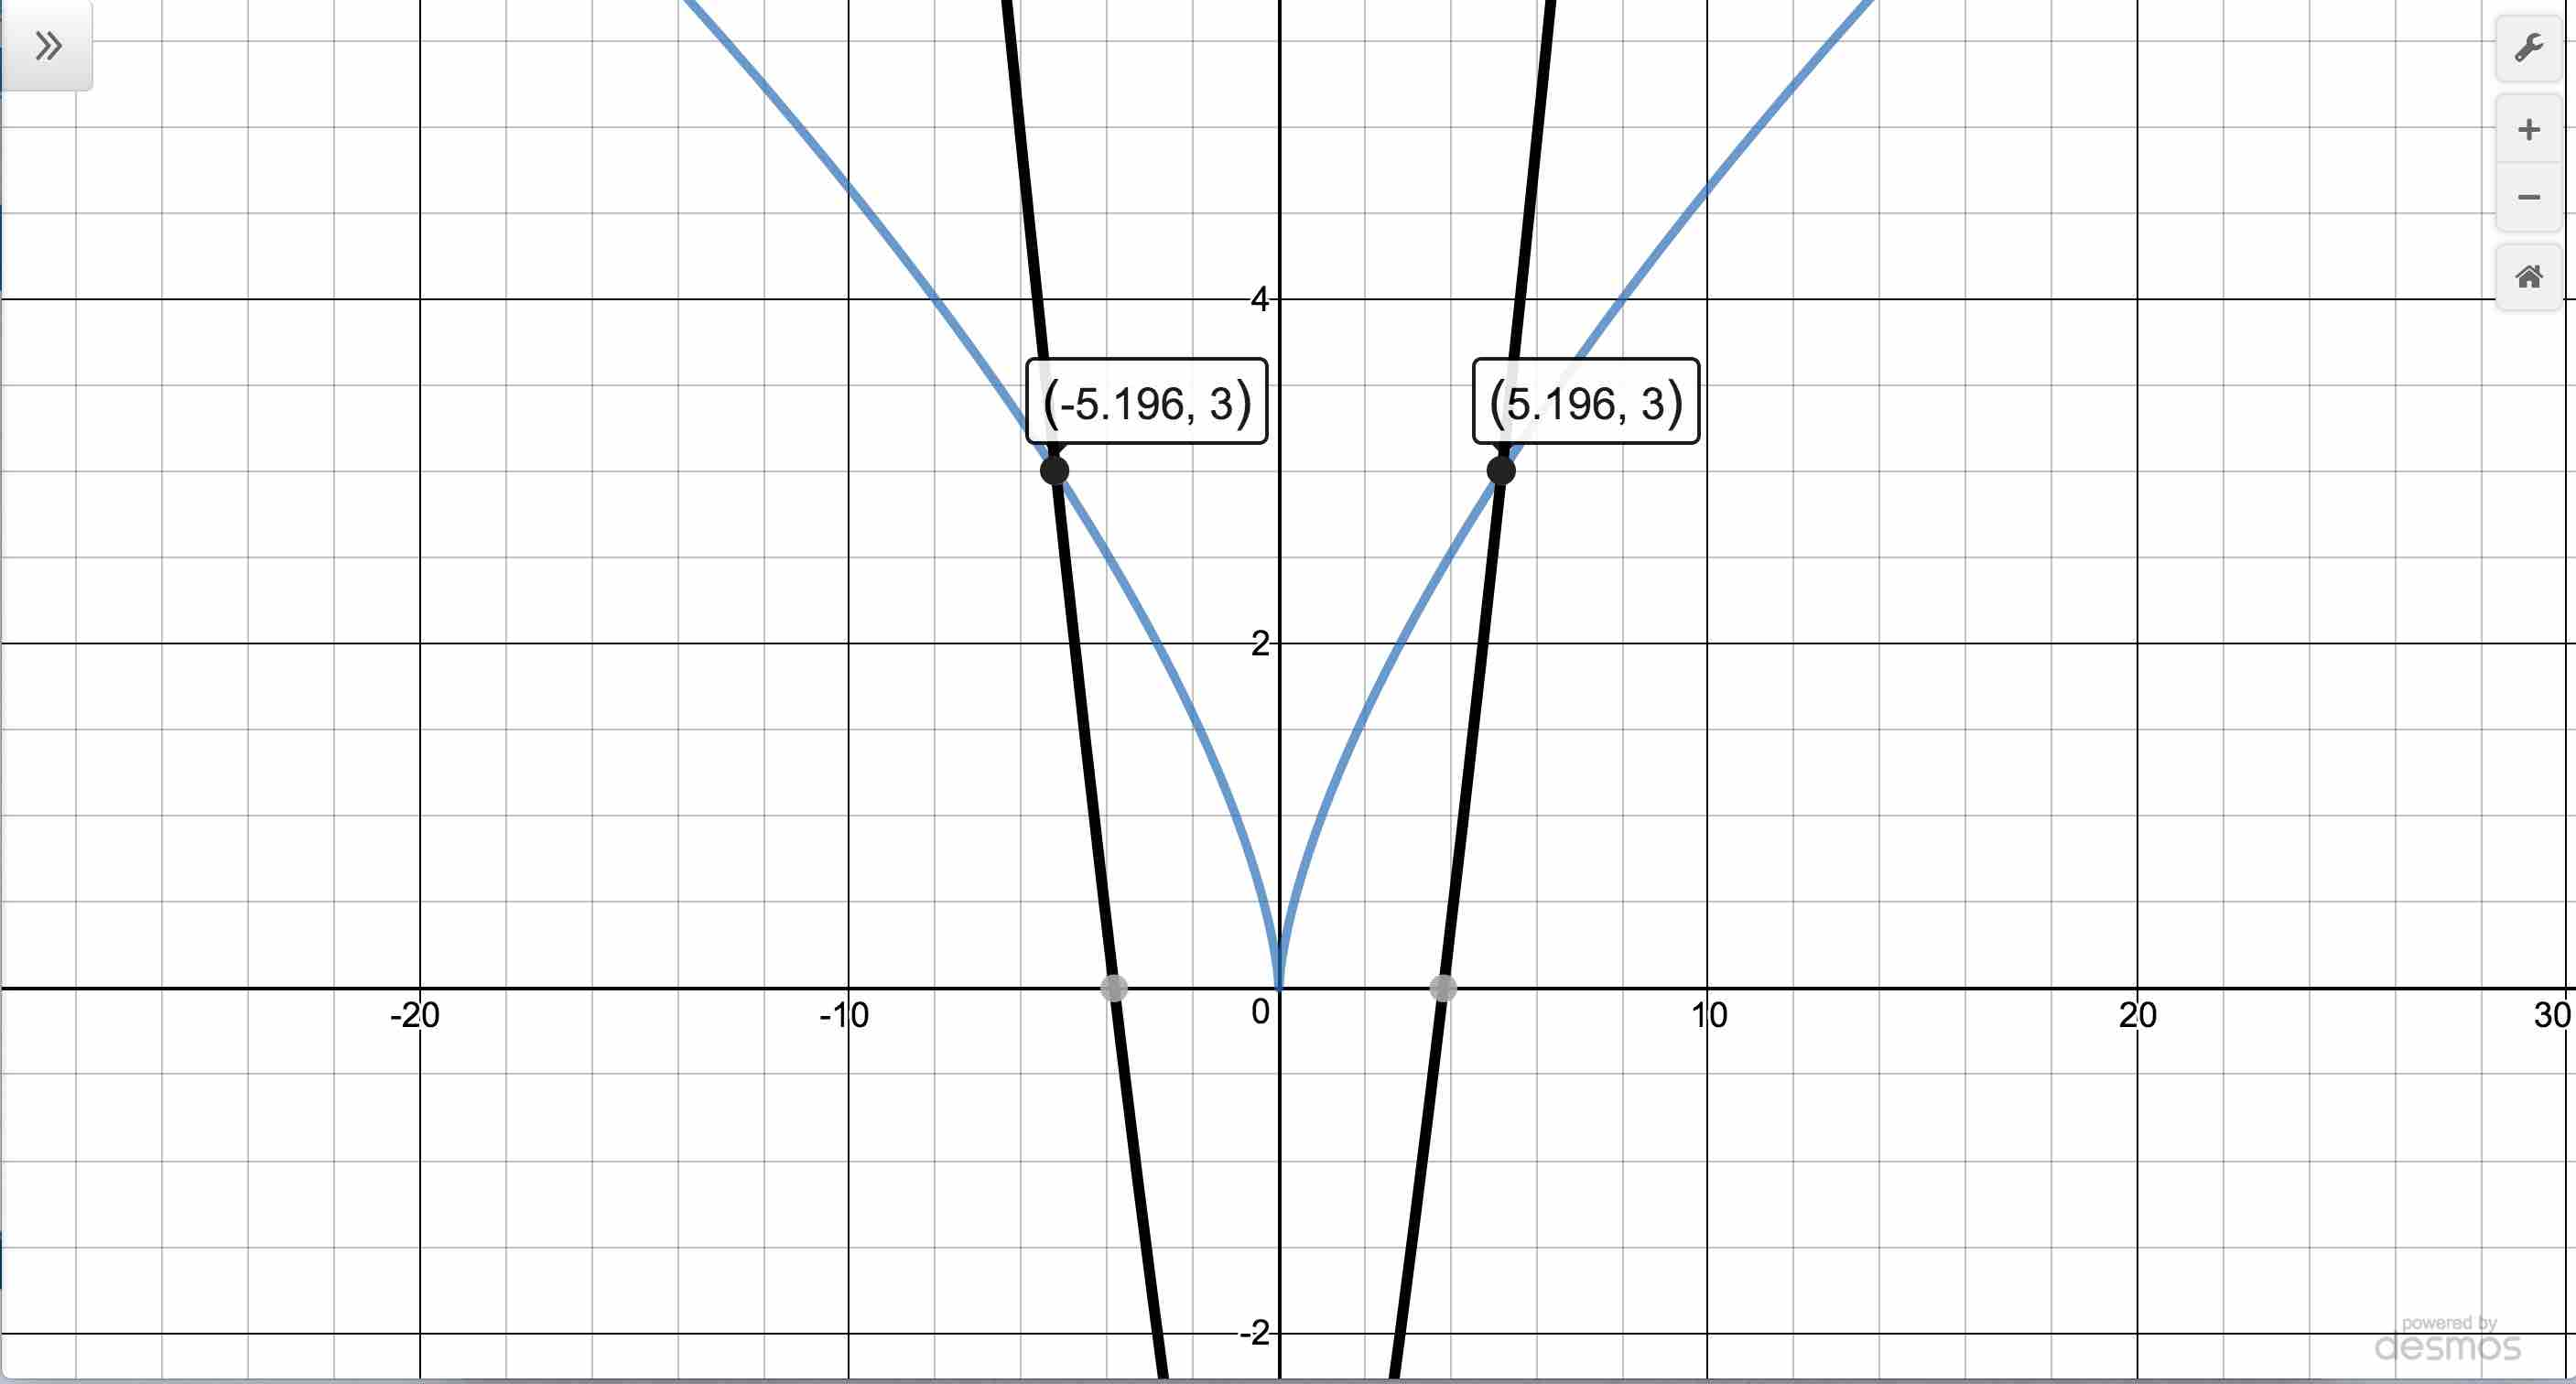
\includegraphics[width=3in]{./PowerEqIneqGraphics/PowerIneqEx02.jpg}  \\


\end{tabular}

\end{center}

\item  To solve $3 (2-x)^{\frac{1}{3}} \leq x (2-x)^{-\frac{2}{3}}$, we first gather all the nonzero terms to one side and obtain $3 (2-x)^{\frac{1}{3}} - x (2-x)^{-\frac{2}{3}} \leq 0$. Setting $r(x) = 3 (2-x)^{\frac{1}{3}} - x (2-x)^{-\frac{2}{3}}$, we note  since the denominators of the rational exponents are odd, we have no domain concerns owing to even indexed roots.  However, the negative exponent on the second term indicates a denominator.  Rewriting $r(x)$ with positive exponents, we obtain \[r(x) =  3 (2-x)^{\frac{1}{3}} - \frac{x}{(2-x)^{\frac{2}{3}}}\]  Setting the denominator equal to zero we get $(2-x)^{\frac{2}{3}} = 0$, which reduces to  $2-x=0$, or $x=2$.  Hence, the domain of $r$ is $(-\infty, 2) \cup (2, \infty)$. 

To find the zeros of $r$, we set $r(x) = 0$, so we set about solving \[3 (2-x)^{\frac{1}{3}} - \frac{x}{(2-x)^{\frac{2}{3}}} = 0.\] Clearing denominators, we get $3  (2-x)^{\frac{1}{3}} (2-x)^{\frac{2}{3}} - x = 0$.  Since the denominators of the exponents are odd, we may use Theorem \ref{exponentprops} to simplify this to $3(2-x)^{1} - x = 0$, and obtain $6-4x = 0$ or $x = \frac{3}{2}$.  In order for us to be able to more easily determine the sign of $r(x)$ at the test values, we rewrite $r(x)$ as a single term.\footnote{This also gives us a chance to review some good intermediate algebra!}  There are two schools of thought on how to proceed, so we demonstrate both.


\begin{itemize}

\item  \textit{Factoring Approach.}  From $r(x) = 3 (2-x)^{\frac{1}{3}} - x (2-x)^{-\frac{2}{3}}$, we note that the quantity $(2-x)$ is common to both terms.  When we factor out common factors, we factor out the quantity with the \textit{smaller} exponent.  In this case, since $-\frac{2}{3} < \frac{1}{3}$, we factor $(2-x)^{-\frac{2}{3}}$ from both quantities.  While it may seem odd to do so, we need to factor $(2-x)^{-\frac{2}{3}}$ \textit{from} $(2-x)^{\frac{1}{3}}$, which results in subtracting the exponent $-\frac{2}{3}$ from $\frac{1}{3}$.  We proceed using the usual properties of exponents.

\[ \begin{array}{rclr}

r(x)  & = & 3 (2-x)^{\frac{1}{3}} - x (2-x)^{-\frac{2}{3}} & \\ [3pt]
      & = & (2-x)^{-\frac{2}{3}} \left[ 3 (2-x)^{\frac{1}{3} - \left(-\frac{2}{3}\right)} - x\right] & \\ [6pt]
      & = & (2-x)^{-\frac{2}{3}}\left[3(2-x)^{\frac{3}{3}} - x\right] & \\ [3pt]
      & = & (2-x)^{-\frac{2}{3}}\left[3(2-x)^{1} - x\right] &  \\ [3pt]
      & = & (2-x)^{-\frac{2}{3}}\left(6-4x\right) & \\ [3pt]
      & = & (2-x)^{-\frac{2}{3}}\left(6-4x\right) & \\
      
\end{array}\]

Written without negative exponents, we have $r(x) = \dfrac{6-4x}{(2-x)^{\frac{2}{3}}}$.

\newpage

\item \textit{Common Denominator Approach.}  We rewrite 

\[ \begin{array}{rclr}

r(x)  & = & 3 (2-x)^{\frac{1}{3}} - x (2-x)^{-\frac{2}{3}} & \\ [3pt]
      & = & 3 (2-x)^{\frac{1}{3}} - \dfrac{x}{(2-x)^{\frac{2}{3}}} & \\ [10pt]
      & = & \dfrac{3 (2-x)^{\frac{1}{3}}(2-x)^{\frac{2}{3}}}{(2-x)^{\frac{2}{3}}} - \dfrac{x}{(2-x)^{\frac{2}{3}}} & \text{common denominator} \\ [10pt]
      & = & \dfrac{3 (2-x)^{\frac{1}{3} + \frac{2}{3}}}{(2-x)^{\frac{2}{3}}} - \dfrac{x}{(2-x)^{\frac{2}{3}}} & \text{Theorem \ref{exponentprops}}  \\ [10pt]
      & = & \dfrac{3 (2-x)^{\frac{3}{3}}}{(2-x)^{\frac{2}{3}}} - \dfrac{x}{(2-x)^{\frac{2}{3}}} & \\ [10pt]
      & = & \dfrac{3 (2-x)^1}{(2-x)^{\frac{2}{3}}} - \dfrac{x}{(2-x)^{\frac{2}{3}}} &  \\ [10pt]
      & = & \dfrac{3 (2-x) - x}{(2-x)^{\frac{2}{3}}} & \\ [10pt]
      & = & \dfrac{6-4x}{(2-x)^{\frac{2}{3}}} & \\

       
\end{array}\]


\end{itemize}

Using either approach, we end up with the same, simpler, expression for $r(x)$ and we use that to create our sign diagram as shown below on the left.  We find $r(x) \leq 0$ on $\left[\frac{3}{2},2\right) \cup (2, \infty)$.  To check this graphically, we set $f(x)=3 (2-x)^{\frac{1}{3}}$ (the lighter curve) and $g(x) = x (2-x)^{-\frac{2}{3}}$ (the darker curve). We confirm that the graphs intersect at $x=\frac{3}{2}$ and the graph of $f$ is below the graph of $g$ for $x > \frac{3}{2}$, with the exception of $x=2$ where it appears the graph of $g$ has a vertical asymptote. 

\begin{center}

\begin{tabular}{m{2in}m{2.5in}}

\begin{mfpic}[10]{-5}{5}{-1}{2}

\arrow \reverse \arrow \polyline{(-5,0),(5,0)}

\xmarks{-2,2}

\tlabel[cc](-3.5,1){$(+)$}

\tlabel[cc](-2,-1.25){$\frac{3}{2}$}

\tlabel[cc](-2,1){$0$}

\tlabel[cc](0,1){$(-)$}

\tlabel[cc](2,-1){$2$}

\tlabel[cc](2,1){\textinterrobang}

\tlabel[cc](3.5,1){$(-)$}

\end{mfpic}

&

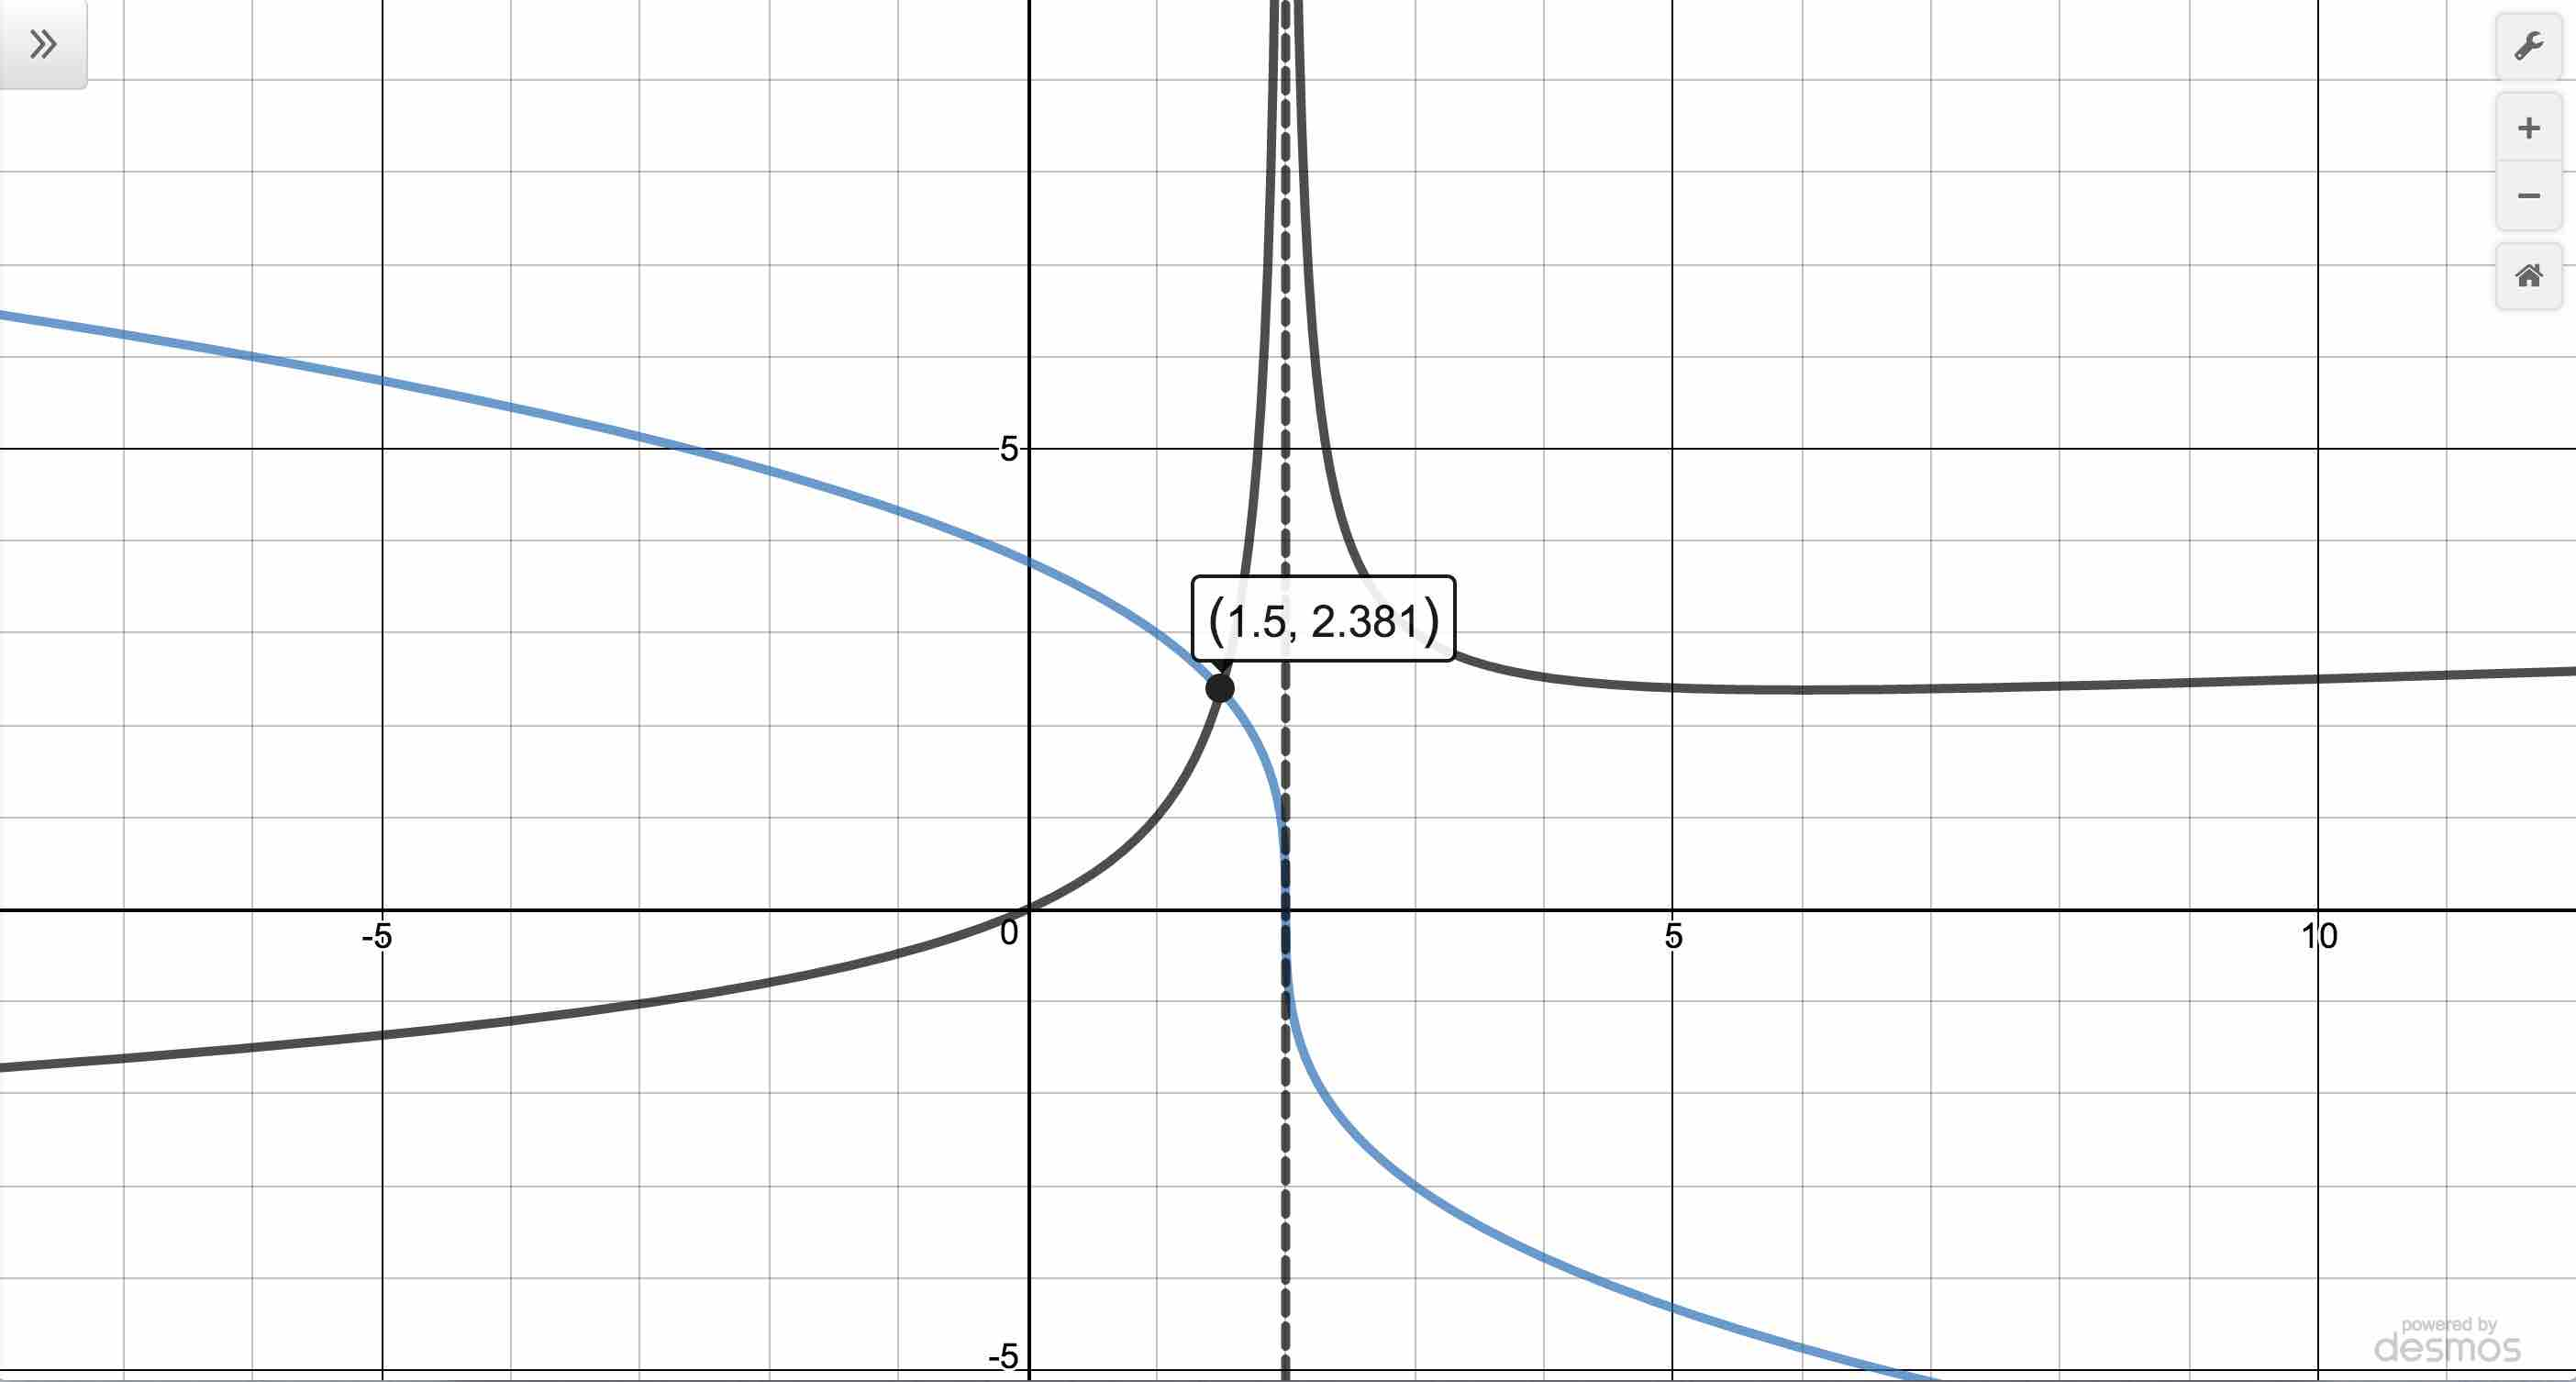
\includegraphics[width=3in]{./PowerEqIneqGraphics/PowerIneqEx03.jpg} \\


\end{tabular}

\end{center}


\item While it may be tempting to begin solving  our last inequality by clearing denominators, owing to the odd root, the quantity $3(t-4)^{\frac{1}{3}}$ can be both positive and negative for different values of $t$.  This means that if we chose to multiply both sides of our inequality by this quantity, we have no guarantee if the inequality would be preserved.  Hence we proceed as usual by gathering all the nonzero terms to one side, and,  with the ultimate goal of creating a sign diagram, get common denominators.  

\[ \begin{array}{rclr}

(t-4)^{\frac{2}{3}} & \geq &  - \dfrac{2t}{3(t-4)^{\frac{1}{3}}} & \\


(t-4)^{\frac{2}{3}} + \dfrac{2t}{3(t-4)^{\frac{1}{3}}}  & \geq & 0 \\

\dfrac{ (t-4)^{\frac{2}{3}} \cdot 3(t-4)^{\frac{1}{3}} }{3(t-4)^{\frac{1}{3}}}  + \dfrac{2t}{3(t-4)^{\frac{1}{3}}} & \geq & 0 & \text{common denominator} \\

\dfrac{3(t-4)^{\frac{2}{3}+\frac{1}{3}}}{3(t-4)^{\frac{1}{3}}}  + \dfrac{2t}{3(t-4)^{\frac{1}{3}}} & \geq & 0 & \text{Theorem \ref{exponentprops}} \\ 

\dfrac{3(t-4)^{1}}{3(t-4)^{\frac{1}{3}}}  + \dfrac{2t}{3(t-4)^{\frac{1}{3}}} & \geq & 0 & \\ 

\dfrac{3(t-4) + 2t}{3(t-4)^{\frac{1}{3}}}   & \geq & 0 & \\ 

\dfrac{5t-12}{3(t-4)^{\frac{1}{3}}}   & \geq & 0 & \\ 

\end{array} \]

We identify $r(t)$ as the left hand side of the inequality and see right away we must exclude $t=4$ from the domain owing to the quantity $(t-4)$ in the denominator.  As we have already mentioned, the root here ($3$) is odd, so we have no domain issues stemming from that.  To find the zeros of $r$, we set $r(t) = 0$ which quickly reduces to solving $5t-12 = 0$.  We get $t = \frac{12}{5}$.    From the sign diagram, we find $r(t) \geq 0$ on $\left(-\infty, \frac{5}{12} \right] \cup (4, \infty)$.  Graphing $f(t) = (t-4)^{\frac{2}{3}}$ (the lighter curve) and $g(t) = -\frac{2t}{3(t-4)^{\frac{1}{3}}}$ (the darker curve), we see the graph of $f$ is above the graph of $g$ for $t < 2.4$ and again for $t > 4$, with an intersection point at $t=2.4 = \frac{12}{5}$. 

\begin{center}

\begin{tabular}{m{2in}m{2.5in}}

\begin{mfpic}[10]{-5}{5}{-1}{2}

\arrow \reverse \arrow \polyline{(-5,0),(5,0)}

\xmarks{-2,2}

\tlabel[cc](-3.5,1){$(+)$}

\tlabel[cc](-2,-1.25){$\frac{12}{5}$}

\tlabel[cc](-2,1){$0$}

\tlabel[cc](0,1){$(-)$}

\tlabel[cc](2,-1){$4$}

\tlabel[cc](2,1){\textinterrobang}

\tlabel[cc](3.5,1){$(+)$}

\end{mfpic}

&

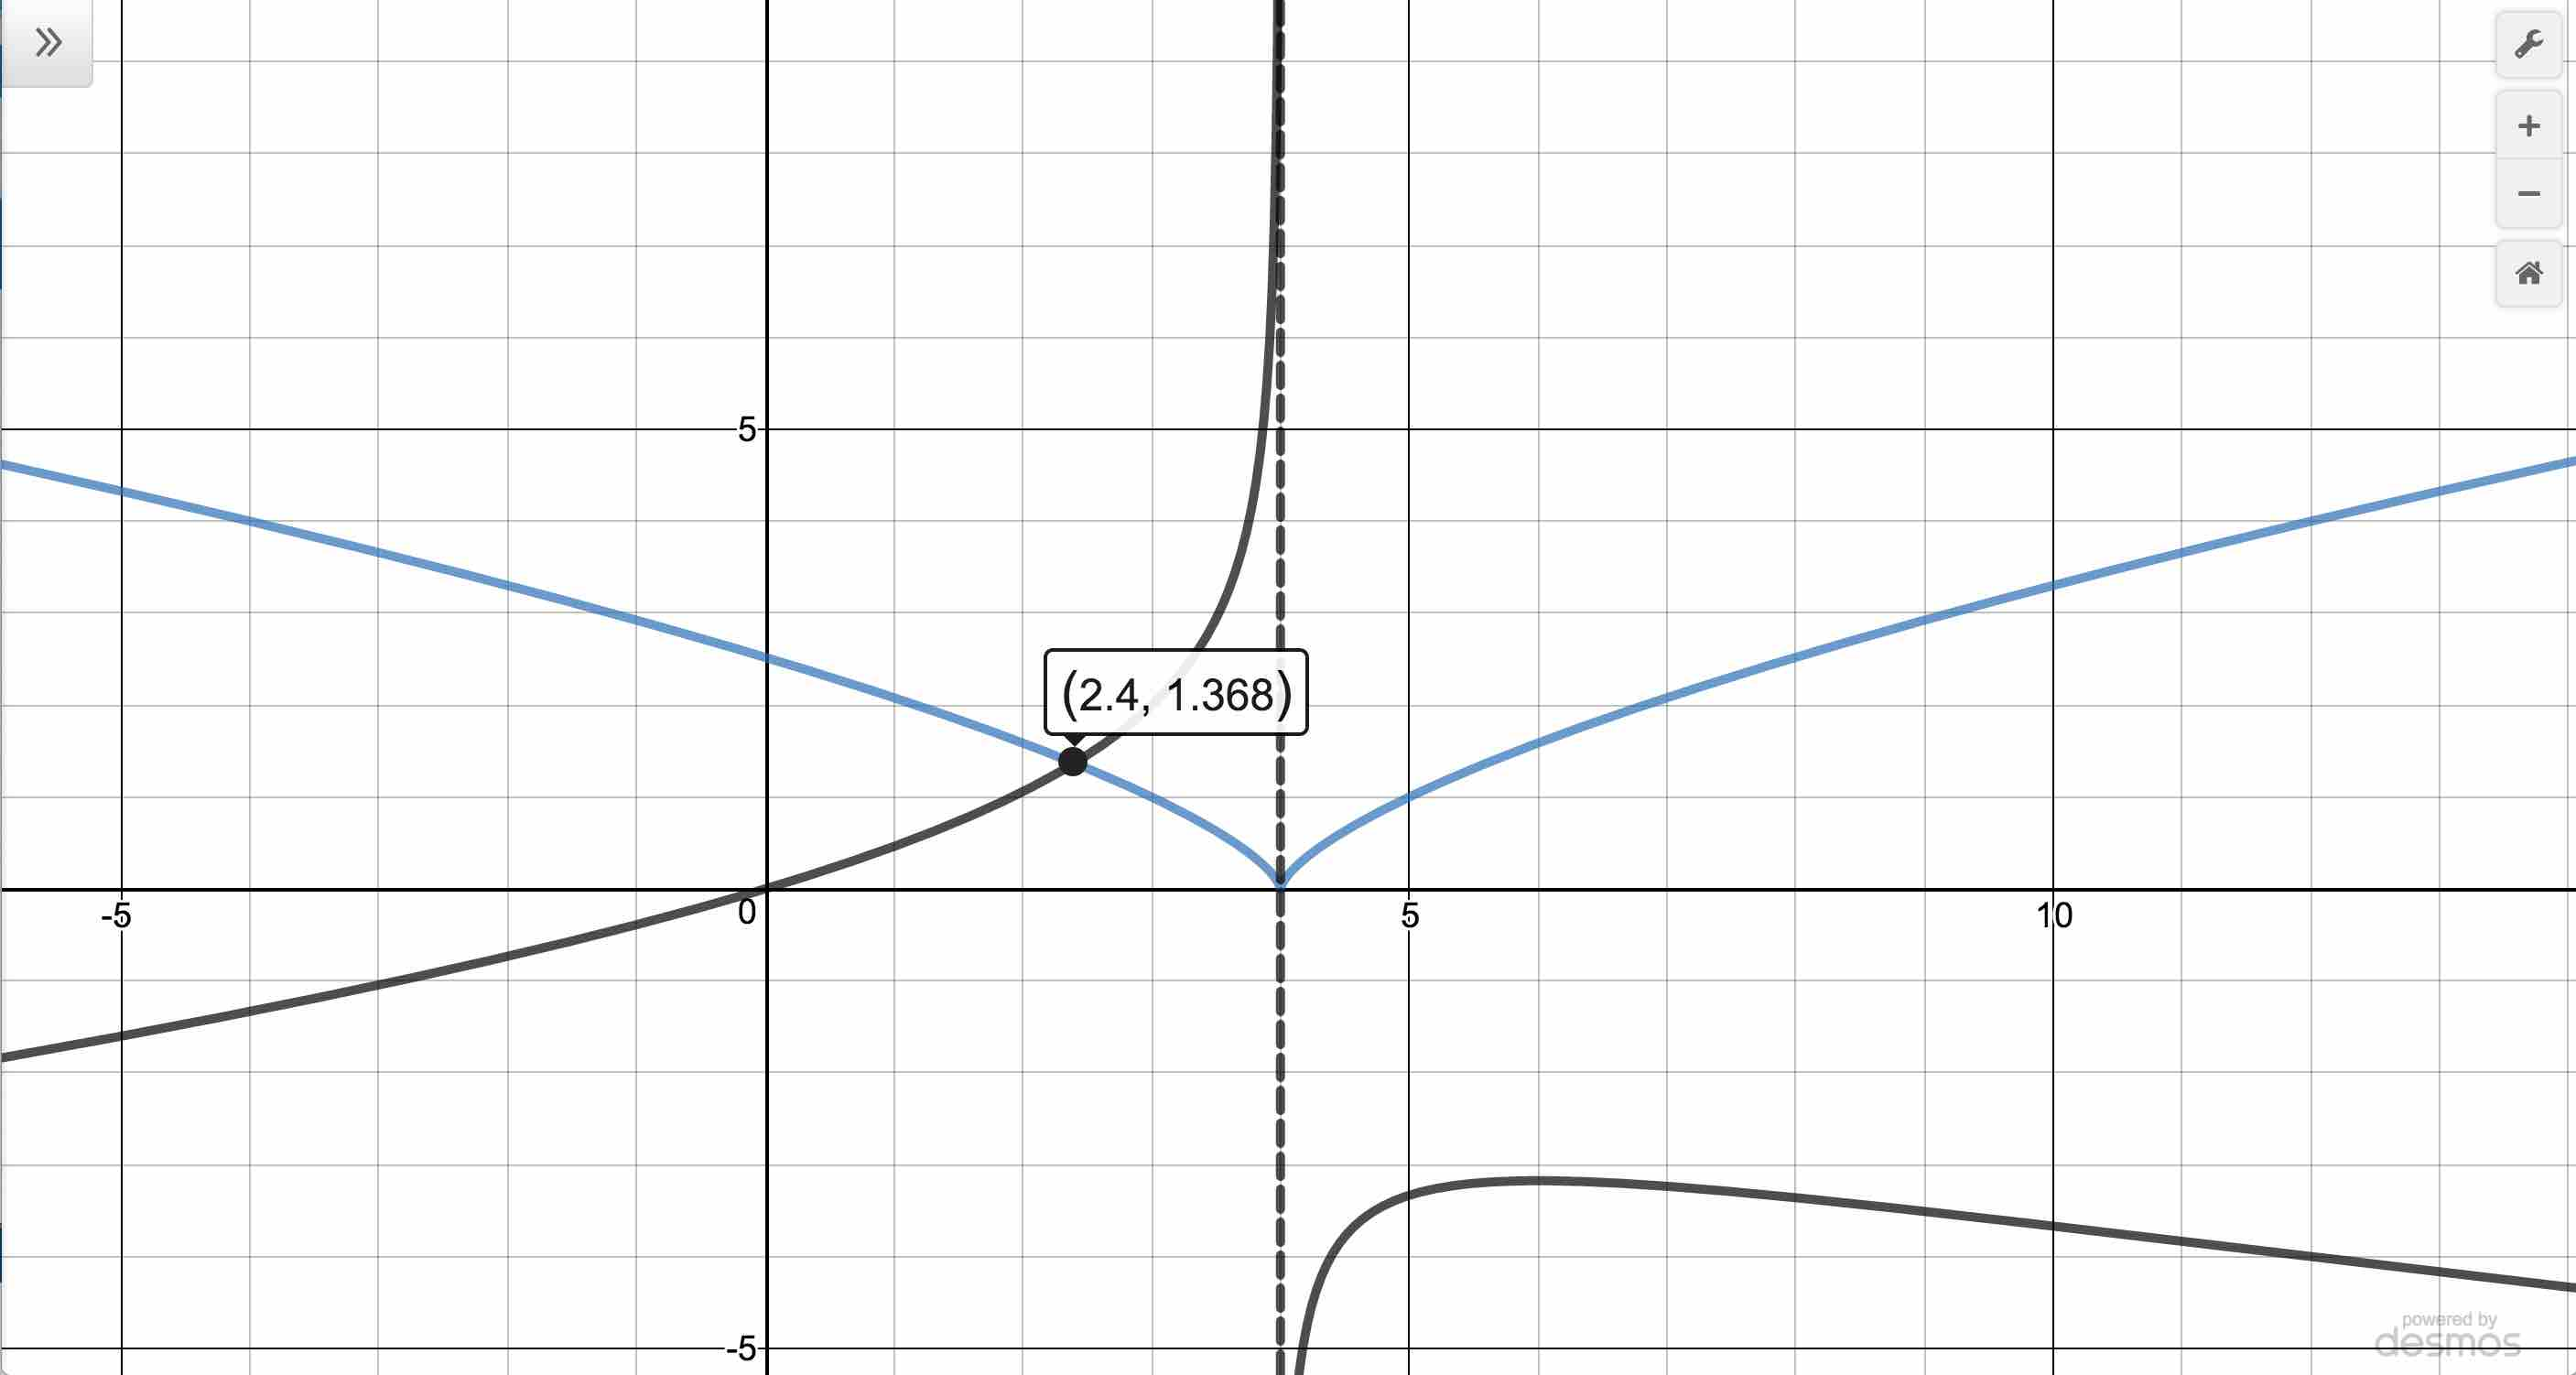
\includegraphics[width=3in]{./PowerEqIneqGraphics/PowerIneqEx04.jpg} \\


\end{tabular}

\end{center}



\end{enumerate}

\qed

\end{example}

\newpage

Note that in Example \ref{powerineqex} number \ref{third}, since $(2-x)^{\frac{2}{3}}$ is always positive  for $x \neq 2$ (owing to the squared exponent), we \textit{could} have short-cut the sign diagram, choosing to  clear denominators instead:

\[ \begin{array}{rclr}

3 (2-x)^{\frac{1}{3}} & \leq & x (2-x)^{-\frac{2}{3}} & \\

3 (2-x)^{\frac{1}{3}} & \leq & \dfrac{x}{(2-x)^{\frac{2}{3}}} & \\

\left[3 (2-x)^{\frac{1}{3}} \right] \left[  (2-x)^{\frac{2}{3}}\right]& \leq & \dfrac{x}{(2-x)^{\frac{2}{3}}}  \left[  (2-x)^{\frac{2}{3}}\right]&  \text{provided $x \neq 2$} \\
3 (2-x)^{\frac{1}{3}} (2-x)^{\frac{2}{3}} & \leq & x&  \\

3 (2-x)^{\frac{1}{3}+\frac{2}{3}} & \leq & x& \\

3(2-x) & \leq & x  & \\ \end{array} \]

Hence, we get $6-3x \leq x$ or $x \geq \frac{3}{2}$, provided $x \neq 2$. This matches our solution $\left[\frac{3}{2},2\right) \cup (2, \infty)$.  If, on the other hand, we tried this same manipulation with number \ref{fourth}, we would clear denominators, assuming $t \neq 4$ to obtain $3(t-4) \geq -2t$ or $t \geq \frac{12}{5}$ which is \textit{not} the correct solution.  The moral of the story is the more you understand, the less you need to rely on memorized processes and the more efficient your solution methodologies can become.  The sign diagram algorithm is a fail-safe method, but, in some cases, may be far from the most efficient one.  It's always best to understand the \textit{why} of a procedure as much as the \textit{how}.  

\newpage

\subsection{Exercises}

%% SKIPPED %% \documentclass{ximera}

\begin{document}
	\author{Stitz-Zeager}
	\xmtitle{TITLE}


In Exercises \ref{powereqineqexfirsta} - \ref{powereqineqexlasta}, solve the equation or inequality.  


\begin{multicols}{2}
\begin{enumerate}


\item $x+1 = (3x+7)^{\frac{1}{2}}$ \label{powereqineqexfirsta}
\item  $2x+1 = (3-3x)^{\frac{1}{2}}$

\setcounter{HW}{\value{enumi}}
\end{enumerate}
\end{multicols}

\begin{multicols}{2}
\begin{enumerate}
\setcounter{enumi}{\value{HW}}


\item  $t + (3t+10)^{0.5} = -2$
\item  $3t+(6-9t)^{0.5}=2$

\setcounter{HW}{\value{enumi}}
\end{enumerate}
\end{multicols}

\begin{multicols}{2}
\begin{enumerate}
\setcounter{enumi}{\value{HW}}

\item $x^{-1.5} = 8$
\item $2x - 1 =  (x + 1)^{-0.5}$

\setcounter{HW}{\value{enumi}}
\end{enumerate}
\end{multicols}

\begin{multicols}{2}
\begin{enumerate}
\setcounter{enumi}{\value{HW}}

\item $t^{\frac{2}{3}} = 4$
\item $(t - 2)^{\frac{1}{2}} + (t - 5)^{\frac{1}{2}} = 3$

\setcounter{HW}{\value{enumi}}
\end{enumerate}
\end{multicols}

\begin{multicols}{2}
\begin{enumerate}
\setcounter{enumi}{\value{HW}}

\item $(2x+1)^{\frac{1}{2}} = 3 + (4-x)^{\frac{1}{2}}$
\item  $5 - (4-2x)^{\frac{2}{3}} = 1$

\setcounter{HW}{\value{enumi}}
\end{enumerate}
\end{multicols}

\begin{multicols}{2}
\begin{enumerate}
\setcounter{enumi}{\value{HW}}

\item  $2t^{\frac{2}{3}} = 6 - t^{\frac{1}{3}}$  % $t=-8, \frac{27}{8}}$
\item  $2t^{\frac{1}{3}} = 1-3t^{\frac{2}{3}} $  % $t=-1, \frac{1}{27}$

\setcounter{HW}{\value{enumi}}
\end{enumerate}
\end{multicols}

\begin{multicols}{2}
\begin{enumerate}
\setcounter{enumi}{\value{HW}}

\item $2x^{1.5} = 15x^{0.75} + 8$  % $x=16$

\item  $35x^{-0.75} = x^{-1.5} +216$ % $x = \frac{1}{81}, \frac{1}{16}$

\setcounter{HW}{\value{enumi}}
\end{enumerate}
\end{multicols}

\begin{multicols}{2}
\begin{enumerate}
\setcounter{enumi}{\value{HW}}


\item  $10-\sqrt{t-2} \leq 11$ \vphantom{$t^{\frac{2}{3}} \leq 4$}
\item  $t^{\frac{2}{3}} \leq 4$ % $[-8,8]$

\setcounter{HW}{\value{enumi}}
\end{enumerate}
\end{multicols}

\begin{multicols}{2}
\begin{enumerate}
\setcounter{enumi}{\value{HW}}


\item  $\sqrt[3]{x} \leq x$   \vphantom{$(2-3x)^{\frac{1}{3}} > 3x$}
\item  $(2-3x)^{\frac{1}{3}} > 3x$  %$\left(-\infty, \frac{1}{3} \right)$

\setcounter{HW}{\value{enumi}}
\end{enumerate}
\end{multicols}

\begin{multicols}{2}
\begin{enumerate}
\setcounter{enumi}{\value{HW}}


\item  $(t^2-1)^{-\frac{1}{2}} \geq 2$  %$\left[ -\frac{\sqrt{5}}{2}, -1\right) \cup \left(1, \frac{\sqrt{5}}{2}\right]$
\item   $(t^2-1)^{-\frac{1}{3}} \leq 2$  %$\left[ -\frac{3\sqrt{2}}{4}, -1\right) \cup (-1,1) \cup \left(1, \frac{3\sqrt{2}}{4}\right]$

\setcounter{HW}{\value{enumi}}
\end{enumerate}
\end{multicols}

\begin{multicols}{2}
\begin{enumerate}
\setcounter{enumi}{\value{HW}}


\item  $3(x-1)^{\frac{1}{3}} +x (x-1)^{-\frac{2}{3}} \geq 0$ % $\left[ \frac{3}{4}, 1\right) \cup (1, \infty)$

\item $3(x-1)^{\frac{2}{3}} +2x (x-1)^{-\frac{1}{3}} \geq 0$ % $\left( -\infty, \frac{3}{5} \right] \cup (1, \infty)$

\setcounter{HW}{\value{enumi}}
\end{enumerate}
\end{multicols}


\begin{multicols}{2}
\begin{enumerate}
\setcounter{enumi}{\value{HW}}


\item  $2 (t-2)^{-\frac{1}{3}} -\frac{2}{3} t(t-2)^{-\frac{4}{3}} \leq 0$ \vphantom{$-\frac{4}{3} (t-2)^{-\frac{4}{3}} + \frac{8}{9} t (t-2)^{-\frac{7}{3}} \geq 0$}
\item  $-\frac{4}{3} (t-2)^{-\frac{4}{3}} + \frac{8}{9} t (t-2)^{-\frac{7}{3}} \geq 0$

\setcounter{HW}{\value{enumi}}
\end{enumerate}
\end{multicols}

\begin{multicols}{2}
\begin{enumerate}
\setcounter{enumi}{\value{HW}}


\item  $2x^{-\frac{1}{3}}(x-3)^{\frac{1}{3}} + x^{\frac{2}{3}} (x-3)^{-\frac{2}{3}} \geq 0$
\item $\sqrt[3]{x^{3} + 3x^{2} - 6x - 8} > x + 1$ \vphantom{ $2x^{-\frac{1}{3}}(x-3)^{\frac{1}{3}} + x^{\frac{2}{3}} (x-3)^{-\frac{2}{3}} \geq 0$}


\setcounter{HW}{\value{enumi}}
\end{enumerate}
\end{multicols}

\begin{multicols}{2}
\begin{enumerate}
\setcounter{enumi}{\value{HW}}

\item $4(7-t)^{0.75} - 3t(7-t)^{-0.25} \leq 0$  \vphantom{$4t^{0.75}(t - 3)^{-\frac{2}{3}} +9t^{-0.25}(t - 3)^{\frac{1}{3}} < 0$} %$[4, \infty)$

\item $4t^{0.75}(t - 3)^{-\frac{2}{3}} +9t^{-0.25}(t - 3)^{\frac{1}{3}} < 0$

\setcounter{HW}{\value{enumi}}
\end{enumerate}
\end{multicols}

\begin{enumerate}
\setcounter{enumi}{\value{HW}}


\item $x^{-\frac{1}{3}} (x-3)^{-\frac{2}{3}} - x^{-\frac{4}{3}} (x-3)^{-\frac{5}{3}} (x^2-3x+2) \geq 0$  \vphantom{$\frac{2}{3}(t + 4)^{\frac{3}{5}}(t - 2)^{-\frac{1}{3}} + \frac{3}{5}(t + 4)^{-\frac{2}{5}}(t - 2)^{\frac{2}{3}} \geq 0$ }
\item $\frac{2}{3}(t + 4)^{\frac{3}{5}}(t - 2)^{-\frac{1}{3}} + \frac{3}{5}(t + 4)^{-\frac{2}{5}}(t - 2)^{\frac{2}{3}} \geq 0$ \label{powereqineqexlasta}

\setcounter{HW}{\value{enumi}}
\end{enumerate}




\begin{enumerate}
\setcounter{enumi}{\value{HW}}
\item The Cobb-Douglas production model\footnote{See Example \ref{CobbDouglasEx} for more details on these sorts of models.} for the country of Sasquatchia is $P = 1.25L^{0.4}K^{0.6}$.  Here, $P$ represents the country's production (measured in thousands of Bigfoot  Bullion), $L$ represents the total labor (measured in thousands of hours) and $K$ represents the total investment in capital (measured in Bigfoot Bullion.)

\begin{enumerate}

\item \label{KintermsofLCobbexercise}Let $P = 300$ and solve for $K$ as a function of  $L$.  If $L = 100$, what is $K$?  Interpret each of the quantities in this case.

\item Graph your answer to \ref{KintermsofLCobbexercise} using a graphing utility.  What information does an ordered pair $(L, K)$ on this graph represent?  

\end{enumerate}

\end{enumerate}

\newpage

\subsection{Answers}

\begin{multicols}{3}
\begin{enumerate}


\item $x=3$  \vphantom{ $x = \frac{1}{4}$ }
\item  $x = \frac{1}{4}$
\item  $t=-3$  \vphantom{ $x = \frac{1}{4}$ }

\setcounter{HW}{\value{enumi}}
\end{enumerate}
\end{multicols}

\begin{multicols}{3}
\begin{enumerate}
\setcounter{enumi}{\value{HW}}


\item  $t = -\frac{1}{3}, \; \frac{2}{3}$  \vphantom{$x = \frac{\sqrt{3}}{2}$}
\item $x = \frac{1}{4}$  \vphantom{$x = \frac{\sqrt{3}}{2}$}
\item $x = \frac{\sqrt{3}}{2}$

\setcounter{HW}{\value{enumi}}
\end{enumerate}
\end{multicols}

\begin{multicols}{3}
\begin{enumerate}
\setcounter{enumi}{\value{HW}}


\item $t = \pm 8$
\item $t = 6$
\item  $x = 4$

\setcounter{HW}{\value{enumi}}
\end{enumerate}
\end{multicols}

\begin{multicols}{3}
\begin{enumerate}
\setcounter{enumi}{\value{HW}}
 
\item  $x=-2, 6$  \vphantom{$t=-8, \frac{27}{8}$}
\item   $t=-8, \frac{27}{8}$
\item   $t=-1, \frac{1}{27}$   \vphantom{$t=-8, \frac{27}{8}$}

\setcounter{HW}{\value{enumi}}
\end{enumerate}
\end{multicols}

\begin{multicols}{3}
\begin{enumerate}
\setcounter{enumi}{\value{HW}}

\item $x=16$ \vphantom{$x = \frac{1}{81}, \frac{1}{16}$}
\item  $x = \frac{1}{81}, \frac{1}{16}$
\item  $[2, \infty)$   \vphantom{$x = \frac{1}{81}, \frac{1}{16}$}


\setcounter{HW}{\value{enumi}}
\end{enumerate}
\end{multicols}

\begin{multicols}{3}
\begin{enumerate}
\setcounter{enumi}{\value{HW}}

\item  $[-8,8]$    \vphantom{ $\left(-\infty, \frac{1}{3} \right)$}
\item  $[-1, 0] \cup [1, \infty)$  \vphantom{ $\left(-\infty, \frac{1}{3} \right)$}
\item $\left(-\infty, \frac{1}{3} \right)$

\setcounter{HW}{\value{enumi}}
\end{enumerate}
\end{multicols}

\begin{multicols}{2}
\begin{enumerate}
\setcounter{enumi}{\value{HW}}

\item $\left[ -\frac{\sqrt{5}}{2}, -1\right) \cup \left(1, \frac{\sqrt{5}}{2}\right]$
\item  $\left(-\infty, -\frac{3\sqrt{2}}{4} \right] \cup (-1,1) \cup \left[ \frac{3\sqrt{2}}{4}, \infty \right)$

\setcounter{HW}{\value{enumi}}
\end{enumerate}
\end{multicols}

\begin{multicols}{2}
\begin{enumerate}
\setcounter{enumi}{\value{HW}}


\item   $\left[ \frac{3}{4}, 1\right) \cup (1, \infty)$

\item $\left( -\infty, \frac{3}{5} \right] \cup (1, \infty)$

\setcounter{HW}{\value{enumi}}
\end{enumerate}
\end{multicols}

\begin{multicols}{2}
\begin{enumerate}
\setcounter{enumi}{\value{HW}}

\item  $(-\infty, 2) \cup (2,3]$
\item  $(2,6]$

\setcounter{HW}{\value{enumi}}
\end{enumerate}
\end{multicols}

\begin{multicols}{2}
\begin{enumerate}
\setcounter{enumi}{\value{HW}}

\item $(-\infty, 0) \cup [2,3) \cup (3, \infty)$
\item $(-\infty, -1)$  


\setcounter{HW}{\value{enumi}}
\end{enumerate}
\end{multicols}

\begin{multicols}{2}
\begin{enumerate}
\setcounter{enumi}{\value{HW}}

\item $[4,7)$  \vphantom{$\left(0, \frac{27}{13} \right)$}
\item $\left(0, \frac{27}{13} \right)$

\setcounter{HW}{\value{enumi}}
\end{enumerate}
\end{multicols}

\begin{multicols}{2}
\begin{enumerate}
\setcounter{enumi}{\value{HW}}
\item $(-\infty, 0) \cup (0,3)$   \vphantom{$(-\infty, -4) \cup \left(-4, -\frac{22}{19}\right] \cup (2, \infty)$}
\item $(-\infty, -4) \cup \left(-4, -\frac{22}{19}\right] \cup (2, \infty)$

\setcounter{HW}{\value{enumi}}
\end{enumerate}
\end{multicols}

\begin{enumerate}
\setcounter{enumi}{\value{HW}}
\item \begin{enumerate}

\item $K=f(L) = (240)^{ \frac{5}{3}} L^{- \frac{2}{3}}$.  $f(100)  \approx 430.2148$.  This means in order for the production level of Sasquatchia to reach 300,000 Bigfoot Bullion with a labor investment of 100,000 hours, the country needs to invest approximately 430 Bigfoot Bullion into capital.


\item If a point $(L,K)$ is on the graph of this function, it means a combination of $L$ thousand hours of labor with an investment of $K$ Bigfoot Bullion into the Sasquatian Economy will result in a production level of 300,000 Bigfoot Bullion.

\centerline{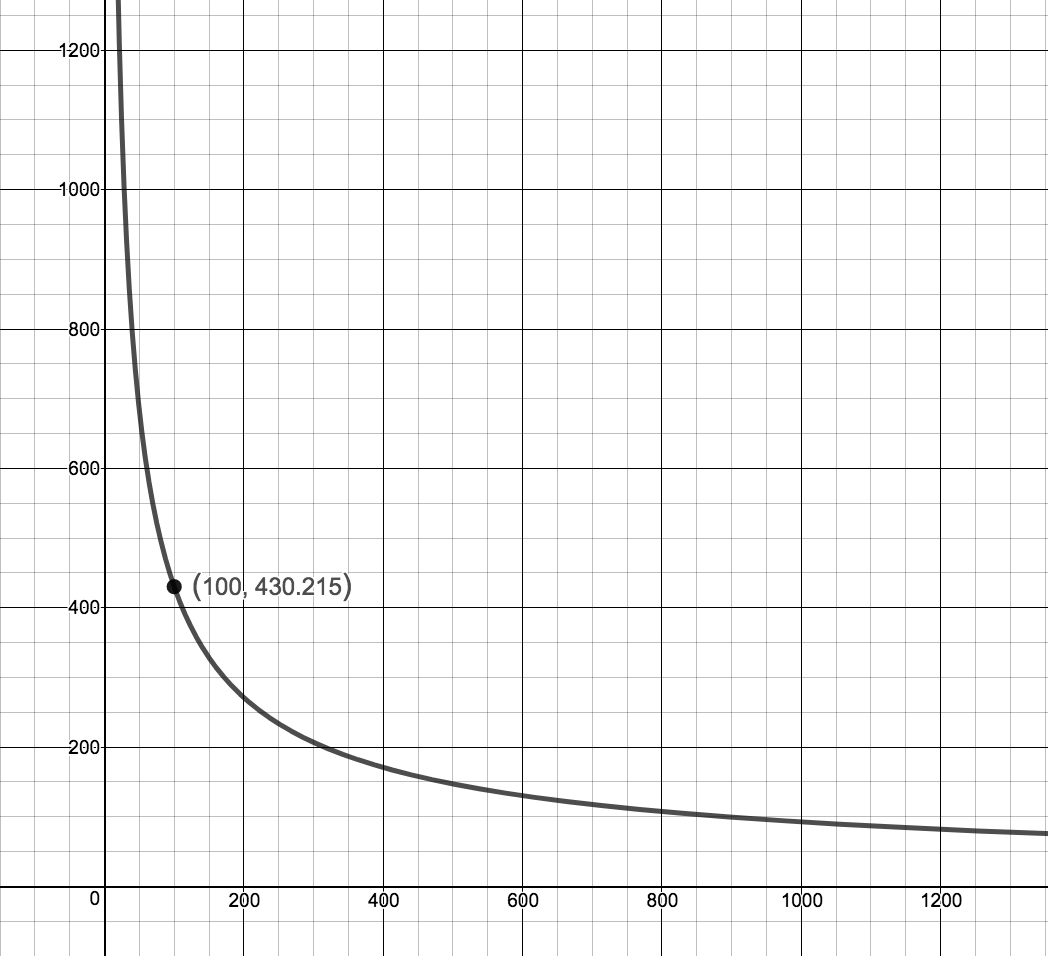
\includegraphics[height=2in]{./PowerEqIneqGraphics/CobbDouglasExercise.jpg}}



\end{enumerate}

\end{enumerate}

\end{document}


\closegraphsfile

\end{document}


\newpage

\end{document}